\section{Linear parameter estimation} 
\label{LinParamEst}

%As can be seen in \eqref{multistate model_smallsignal}, the small signal model of such a multi-state/ multi-input system consists of two Jacobian matrices, one for the states and one for the inputs to the system. It should be emphasized however that these matrices have to be evaluated at the operating points, at $(\bar{x}, \bar{u})$. It is a reasonable statement since the inputs to the model are the small signal values of OD and differential pressures, dp, from the pumps. Therefore the same excitation to the real test setup can be carried out by taking the operating values into account and by adding them to the small signal values. 

The method that describes the linear parameter estimation is shown in \figref{fig:parame_block_lin} below:

\begin{figure}[H]
\centering
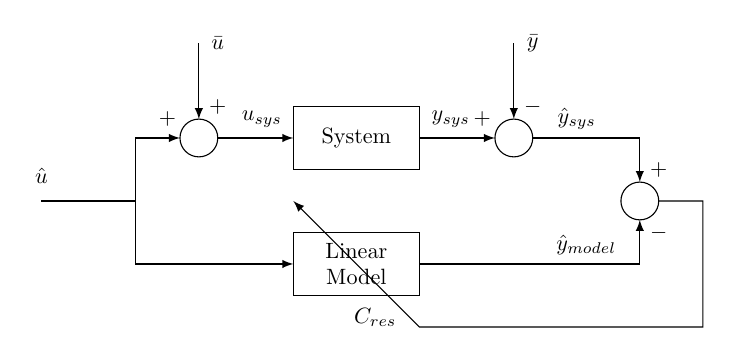
\begin{tikzpicture} [scale=0.8,transform shape]

\draw  (3,-1.5) rectangle (5,-2.5);
\node at (4,-1.8) {Linear};
\node at (4,-2.2) {Model};

\draw  (3,0.5) rectangle (5,-0.5);
\node at (4,0) {System};

\node at (8.8,-1.5) {$-$};
\node at (5.5,0.3) {$y_{sys}$};
\node at (7.5,0.3) {$\hat{y}_{sys}$};
\node at (7.65,-1.7) {$\hat{y}_{model}$};
\node at (4.3,-2.85) {$C_{res}$};
\node at (-1,-0.6) {$\hat{u}$};
\node at (1.8,1.5) {$\bar{u}$};
\node at (2.5,0.3) {$u_{sys}$};
\node at (8.8,-0.5) {$+$};
\node at (1.8,0.5) {$+$};
\node at (6,0.3) {$+$};
\node at (6.8,0.5) {$-$};
\node at (1,0.3) {$+$};
\node at (6.8,1.5) {$\bar{y}$};

\draw  (8.5,-1) ellipse (0.3 and 0.3);
\draw  (6.5,0) ellipse (0.3 and 0.3);
\draw  (1.5,0) ellipse (0.3 and 0.3);

\draw [-latex](5,0) -- (6.2,0);

\draw [-latex](0.5,-1) -- (0.5,0) -- (1.2,0);
\draw [-latex](0.5,-1) -- (0.5,-2) -- (3,-2);
\draw (-1,-1) -- (0.5,-1);
\draw [-latex](5,-2) -- (8.5,-2) -- (8.5,-1.3);
\draw [-latex](8.8,-1) -- (9.5,-1) -- (9.5,-3) -- (5,-3) -- (3,-1);

\draw [-latex](1.8,0) -- (3,0);
\draw [-latex](1.5,1.5) -- (1.5,0.3);
\draw [-latex](6.5,1.5) -- (6.5,0.3);
\draw [-latex](6.8,0) -- (8.5,0) -- (8.5,-0.7);
\end{tikzpicture}% 
\caption{Parameter identification block diagram for the linear system. }
\label{fig:parame_block_lin}
\end{figure}

In this case small-signal inputs are applied to both the test setup and the model.  Now the linearized model is compared to the real system, therefore the operating point is taken into account. Since the linear model is only valid for small deviations around the operating point, the real system has to be excited around the same operating point to obtain identical behavior. In order to achieve it, the operating values are added to both the input and the output such as: 

\begin{equation}
u_{sys} = \bar{u} + \hat{u}
 \label{u_smallsignal}
\end{equation}

\begin{minipage}[t]{0.20\textwidth}
Where\\
\hspace*{8mm} $\hat{u}$ \\
\hspace*{8mm} $\bar{u}$ \\
\hspace*{8mm} $u_{sys}$ 
\end{minipage}
\begin{minipage}[t]{0.68\textwidth}
\vspace*{2mm}
is the small-signal input, \\
is the operating value of the input,\\
is the input to the real-life system. 
\end{minipage}
\begin{minipage}[t]{0.10\textwidth}
\vspace*{2mm}
\textcolor{White}{te}$\unit{bar}$
\textcolor{White}{te}$\unit{bar}$
\textcolor{White}{te}$\unit{bar}$
\end{minipage} 

\begin{equation}
  y_{sys} = \bar{y} + \hat{y}_{sys} 
 \label{u_smallsignal}
\end{equation}

\begin{minipage}[t]{0.20\textwidth}
Where\\
\hspace*{8mm} $\hat{y}_{sys}$ \\
\hspace*{8mm} $\bar{u}_{sys}$ \\
\hspace*{8mm} $y_{sys}$ 
\end{minipage}
\begin{minipage}[t]{0.68\textwidth}
\vspace*{2mm}
is the small-signal output from the real-life system, \\
is the operating value of the output,\\
is the output from the real-life system. 
\end{minipage}
\begin{minipage}[t]{0.10\textwidth}
\vspace*{2mm}
\textcolor{White}{te}$\unit{bar}$
\textcolor{White}{te}$\unit{bar}$
\textcolor{White}{te}$\unit{bar}$
\end{minipage} 

During the linear parameter estimation, the same problem is solved as it is shown in \eqref{ObjectiveFunction}. In this case, however, the parameters are varied according to the comparison of the small-signal outputs.  

\subsection{Model Parameters}
\label{estimateParameters}
In order to obtain a complete model of the physical setup, all the parameters describing the components have to be defined. In \secref{SubSecEstimation} a detailed
description of the known parameters of the system has been done. Nevertheless, in the linearized state-space model more parameters have to be identified
due to the introduction of the operating points values. Hence, in the current chapter a detailed compilation of the unknown parameters of the physical water distribution setup is carried out.


\textbf{Unknown Parameters}
The unknown parameters are the ones related with the form losses, $k_f$, and form friction ,$f$, of the pipes. Despite they are 
provided by the manufactures they need to be estimated. On one hand, the form losses depend on the fittings and bends of the pipes which are not always known. 
On the other hand, the friction losses depend on the inside average roughness of the pipes, $\epsilon$, which can change its value due to passage of time 
and rust generated inside pipes or fittings. 

%The friction and form losses are part of the model of a pipe, and are given by the following equation
%
%\begin{equation}
%  \lambda (q) =  \frac{8fL}{\pi^{2}gD^5} \rho g  |q| q + k_f \frac{8}{\pi^2gD^4} \rho g |q| q
%  \label{frictionestimation}
%\end{equation}

%From the above equation it can be seen that either estimating only for $k_f$ or $f$ will have the same result in the value of $\lambda (q)$.
%Therefore, it has been decided to carry out the estimation of the total value of $\lambda (q)$, hence discarding the respective values of $k_f$ and $f$.

Furthermore, the operating points of the flow through the chords, $\pmb{\bar{z}}$, is also unknown. These values, which correspond to the $8$ flow chords, are introduced in the linearized expression of both pipes 
and valves, see \eqref{lambda_lin} and \eqref{mu_lin}. Thus, not only pipe parameters introduce uncertainties into the system model but also the lack of knowledge of the chord operating points.

Consequently, it has been decided to estimate the total expression for the pressure across the pipes and valves in order to reduce the amount of unknowns in the system.

The system has $15$ pipes in total,  from \eqref{lambda_lin} it can be seen that either tunning for $k_f$, $f$ or $\pmb{\bar{z}}$ it will have the same result for the total
value of the pressure across the pipes, $\lambda(\pmb{{B_1^{T}}}\pmb{z})$. For this reason the pressure across the 15 pipes is estimated.

The linearized valve expression, see \eqref{mu_lin}, consists of the term depending on the chord flows and the one depending on the $OD$. Both terms include the operating 
point of the chord flows inside them, thus, the pressure difference given by both terms has to be estimated. In the system 4 valves take part, 
resulting in 8 unknowns in total. 

The WT connection edge, see \eqref{gamma_lin}, is conformed by two valves and one pump. Although the parameters corresponding to the pump are considered as known, the ones 
corresponding to the valves have to be estimated. Resulting in two more unknowns for the system. 

All in all, the system has $24$ unknown terms which will be calculated following the estimation process described in the next section.
\subsection{Measurements on the test setup}
\label{LinParamEst_measurements}

In order to verify the state-space model derived in \chapref{LinParamEst} with the physical setup, an estimation for the parameters defined in \secref{estimateParameters}
is carried out.

From the system setup, $9$ different relative pressures can be measured, following \figref{systemdiagram} notation the sensors are placed in: 
$n_2$ $n_4$ $n_5$ $n_7$ $n_{10}$ $n_{11}$ $n_{15}$ $n_{16}$ $n_{18}$. However, the estimation will be done only regarding the four PMA relative pressure 
sensors across the end-users and the pressure in the WT, since those are the outputs that will be controlled in \secref{SystemLin_control}. Thus, the estimation will only focus on obtaining the best fit for those sensor outputs relevant in the control part. 

The relationship between pressures, where DpCXX describes the pressure difference for the XX component, is obtained in the same way as \secref{SubSecEstimation} and can be defined as:

\text{\underline{Node 10}}
\vspace{4mm}
\begin {equation}
     y_1 = DpC20 + DpC21  
\end{equation}

\text{\underline{Node 11}}
\vspace{4mm}
\begin {equation}
     y_2 = DpC24
\end{equation}


\text{\underline{Node 15}}
\vspace{4mm}
\begin {equation}
     y_3 = DpC28 + DpC20 
\end{equation}

\text{\underline{Node 15}}
\vspace{4mm}
\begin {equation}
     y_4 = DpC31 
\end{equation}

There is no need to define a relation with a referent point for the WT node, since the pressure across the WT is the state of the state-space model. 

\subsection{Linear Estimation Outcomes}
In \appref{LinResults} the results of the estimation process are shown, where the $24$ terms defining the pressure across the unknowns edges are estimated.
From the tests it can be seen a slightly different behavior between the model and the data from the setup, especially at time $t = 350s$. This dissimilar 
behavior showing up at some time samples could make the model unsuitable for the real setup, thus making it incorrect to be used in a model based control scheme. 

In light of the above considerations, a different approach for the parameter estimation is attempted. In \secref{estimateParameters} it has been described how the unknown pressures across the edges are estimated in order to build up the state-space matrices of the system. Nonetheless, as the estimation did not succeed it has been decided to estimate the final values of the state-space matrices stated in \eqref{statespace_1}, where $M$ is a symmetric matrix, and \eqref{statespace_5}. 

Altogether these matrices sum up to 28 unknown parameters, which are the ones to be estimated. The outputs to be compared with the test setup remain 
the same as in \secref{LinParamEst_measurements}, as well as the toolbox used for estimating.

\textbf{Estimation Data}

As the parameter estimation is based on a linearized model an operating point for the system is chosen. This point is based on the WT being approximately half way full which allows for an equal amount of deviation in both directions. For the chosen operating point, data is gathered from the system while small steps are individually applied to the two main pumps and the opening degree of the PMA valves. In order to use the data for parameter estimation the operating point is subtracted, leaving only small signal values.  

The operating point of the PMA valves is placed at $70\%$ opening corresponding to $63^{\circ}$ and the small signal values for the estimation can be seen in \figref{fig:est_OD_data_final}.

\begin{figure}[H]
\centering
% This file was created by matlab2tikz.
%
%The latest updates can be retrieved from
%  http://www.mathworks.com/matlabcentral/fileexchange/22022-matlab2tikz-matlab2tikz
%where you can also make suggestions and rate matlab2tikz.
%
\definecolor{mycolor1}{rgb}{0.00000,0.44700,0.74100}%
\definecolor{mycolor2}{rgb}{0.85000,0.32500,0.09800}%
\definecolor{mycolor3}{rgb}{0.92900,0.69400,0.12500}%
\definecolor{mycolor4}{rgb}{0.49400,0.18400,0.55600}%
%
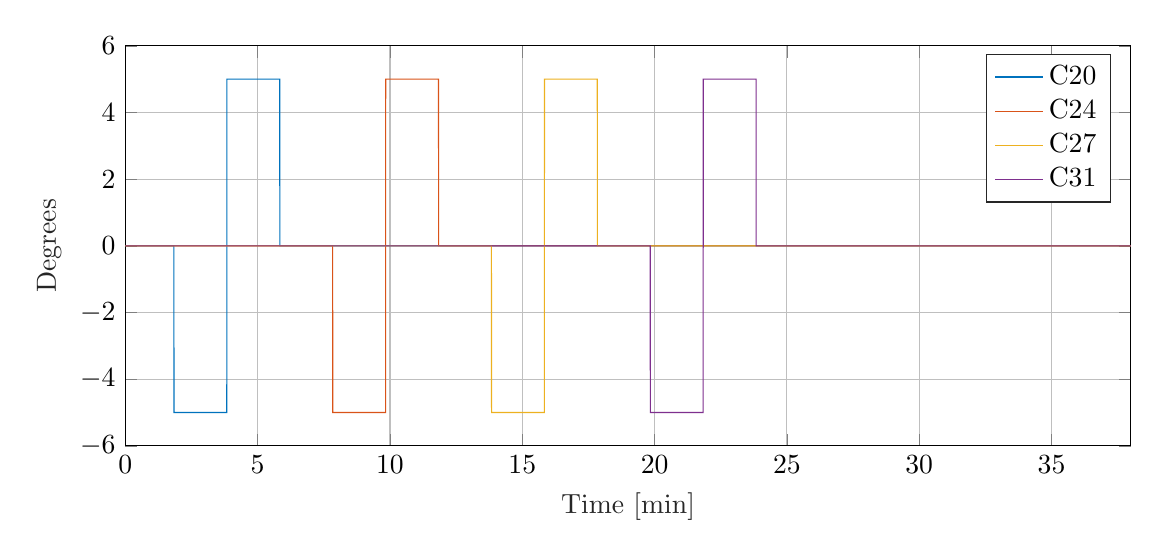
\begin{tikzpicture}

\begin{axis}[%
width=5.028in,
height=2in,
at={(0.758in,0.481in)},
scale only axis,
xmin=0,
xmax=38,
xlabel style={font=\color{white!15!black}},
xlabel={Time [min]},
ymin=-6,
ymax=6,
ylabel style={font=\color{white!15!black}},
ylabel={Degrees},
axis background/.style={fill=white},
%title style={font=\bfseries},
%title={Valve opening degree},
xmajorgrids,
ymajorgrids,
legend style={legend cell align=left, align=left, draw=white!15!black}
]
\addplot [color=mycolor1]
  table[row sep=crcr]{%
0	-4.00248723053664e-11\\
1.83416666666667	-4.00248723053664e-11\\
1.83916666666666	-5.00000000004003\\
3.83416666666667	-5.00000000004003\\
3.83916666666666	4.99999999995997\\
5.83416666666667	4.99999999995997\\
5.83916666666667	-4.00248723053664e-11\\
53.3325	-4.00248723053664e-11\\
};
\addlegendentry{C20}

\addplot [color=mycolor2]
  table[row sep=crcr]{%
0	-4.4146020172775e-11\\
7.83416666666667	-4.4146020172775e-11\\
7.83916666666667	-5.00000000004415\\
9.83416666666667	-5.00000000004415\\
9.83916666666667	4.99999999995585\\
11.8341666666667	4.99999999995585\\
11.8391666666667	-4.4146020172775e-11\\
53.3325	-4.4146020172775e-11\\
};
\addlegendentry{C24}

\addplot [color=mycolor3]
  table[row sep=crcr]{%
0	-4.74145167572715e-11\\
13.8341666666667	-4.74145167572715e-11\\
13.8391666666667	-5.00000000004742\\
15.8341666666667	-5.00000000004742\\
15.8391666666667	4.99999999995258\\
17.8341666666667	4.99999999995258\\
17.8391666666667	-4.74145167572715e-11\\
53.3325	-4.74145167572715e-11\\
};
\addlegendentry{C27}

\addplot [color=mycolor4]
  table[row sep=crcr]{%
0	-4.05933064939745e-11\\
19.8341666666667	-4.05933064939745e-11\\
19.8391666666667	-5.00000000004059\\
21.8341666666667	-5.00000000004059\\
21.8391666666667	4.99999999995941\\
23.8341666666667	4.99999999995941\\
23.8391666666667	-4.05933064939745e-11\\
53.3325	-4.05933064939745e-11\\
};
\addlegendentry{C31}

\end{axis}
\end{tikzpicture}% 
\caption{Small signal values of the opening degrees of the pma valves.}
\label{fig:est_OD_data_final}
\end{figure}

To acheive a 50\% fill level of the WT in steady state combined with the chosen operating point of the valves, the operating point of the two inlet pumps C2 and C16 has to be set at a differential pressure of $\Delta p = 0.2 Bar$. The required operating point is found by experimental tests made on the setup, the small signal values used in the estimation are shown in \figref{fig:est_deltap_data_final}. 

\begin{figure}[H]
\centering
% This file was created by matlab2tikz.
%
%The latest updates can be retrieved from
%  http://www.mathworks.com/matlabcentral/fileexchange/22022-matlab2tikz-matlab2tikz
%where you can also make suggestions and rate matlab2tikz.
%
\definecolor{mycolor1}{rgb}{0.00000,0.44700,0.74100}%
\definecolor{mycolor2}{rgb}{0.85000,0.32500,0.09800}%
%
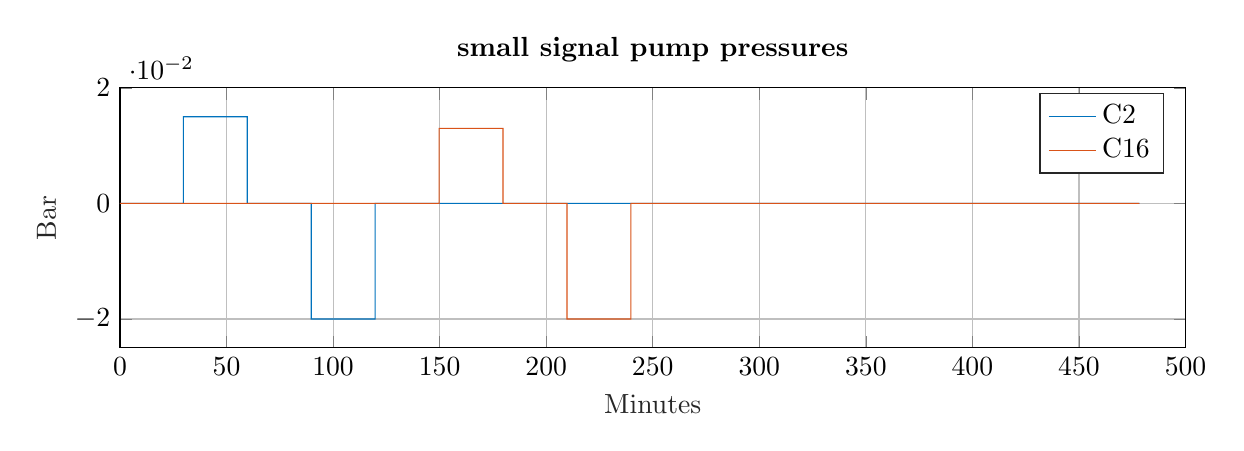
\begin{tikzpicture}

\begin{axis}[%
width=5.328in,
height=1.3in,
at={(1.011in,0.642in)},
scale only axis,
xmin=0,
xmax=500,
xlabel style={font=\color{white!15!black}},
xlabel={Minutes},
ymin=-0.025,
ymax=0.02,
ylabel style={font=\color{white!15!black}},
ylabel={Bar},
axis background/.style={fill=white},
title style={font=\bfseries},
title={small signal pump pressures},
xmajorgrids,
ymajorgrids,
legend style={legend cell align=left, align=left, draw=white!15!black}
]
\addplot [color=mycolor1]
  table[row sep=crcr]{%
0	-0\\
29.7508333333333	-0\\
29.7516666666667	0.0149999999999864\\
59.7508333333333	0.0149999999999864\\
59.7516666666667	-0\\
89.7508333333333	-0\\
89.7516666666667	-0.0200000000000387\\
119.750833333333	-0.0200000000000387\\
119.751666666667	-0\\
478.333333333333	-0\\
};
\addlegendentry{C2}

\addplot [color=mycolor2]
  table[row sep=crcr]{%
0	-0\\
149.750833333333	-0\\
149.751666666667	0.0129999999999768\\
179.750833333333	0.0129999999999768\\
179.751666666667	-0\\
209.750833333333	-0\\
209.751666666667	-0.0200000000000387\\
239.750833333333	-0.0200000000000387\\
239.751666666667	-0\\
478.333333333333	-0\\
};
\addlegendentry{C16}

\end{axis}
\end{tikzpicture}% 
\caption{Small signal values of the differential pressure of the two main pumps.}
\label{fig:est_deltap_data_final}
\end{figure}



\textbf{Estimation Result}

The following figures show the comparison between the data obtained from the lab and the outputs of the model with the estimated parameters.  

\begin{figure}[H]
  \centering
    % This file was created by matlab2tikz.
%
%The latest updates can be retrieved from
%  http://www.mathworks.com/matlabcentral/fileexchange/22022-matlab2tikz-matlab2tikz
%where you can also make suggestions and rate matlab2tikz.
%
\definecolor{mycolor1}{rgb}{0.00000,0.44700,0.74100}%
\definecolor{mycolor2}{rgb}{0.85000,0.32500,0.09800}%
%
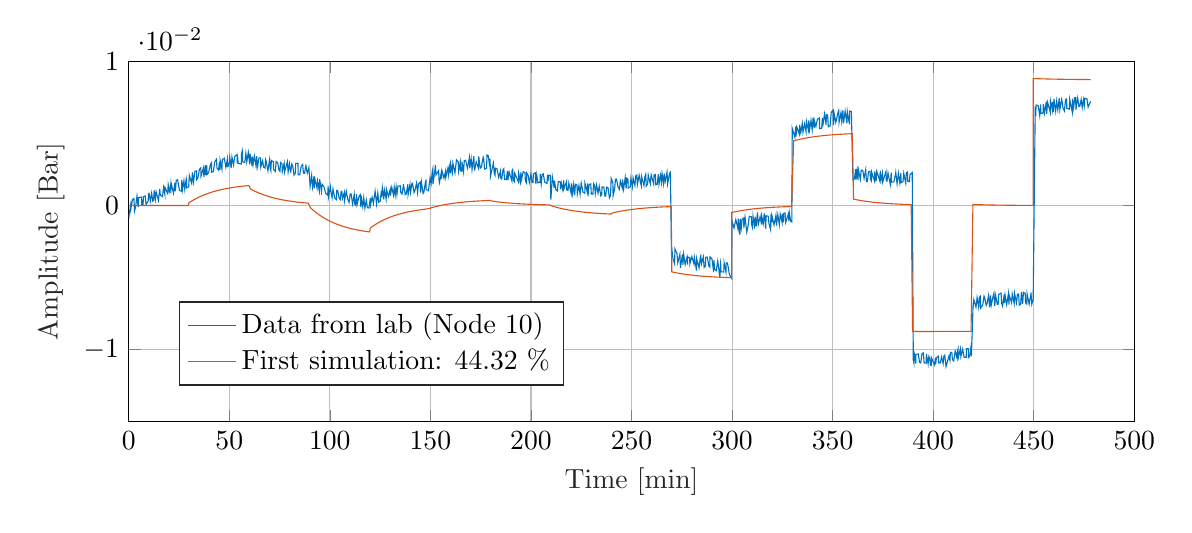
\begin{tikzpicture}

\begin{axis}[%
width=5.028in,
height=1.8in,
at={(1.011in,0.642in)},
scale only axis,
xmin=0,
xmax=500,
xlabel style={font=\color{white!15!black}},
xlabel={Time [min]},
ymin=-0.015,
ymax=0.01,
ylabel style={font=\color{white!15!black}},
ylabel={Amplitude [Bar]},
axis background/.style={fill=white},
%title style={font=\bfseries},
%title={Node 10},
xmajorgrids,
ymajorgrids,
legend style={at={(0.05,0.1)}, anchor=south west, legend cell align=left, align=left, draw=white!15!black}
]
\addplot [color=mycolor1]
  table[row sep=crcr]{%
0.000833333333333333	-0.000504237183846401\\
0.196666666666667	-0.000686935131059913\\
0.986666666666667	5.51665307179927e-05\\
1.10333333333333	-0.000202350575829138\\
1.86333333333333	0.000425782366495597\\
2.59583333333333	0.000486681682232357\\
2.87916666666667	-0.000384178532817164\\
3.4325	-8.92518465969022e-05\\
4.12833333333333	0.000658069756540966\\
4.7075	-0.000108391631539626\\
4.86333333333333	0.00054323104685336\\
6.41416666666667	0.000593690479898448\\
6.51333333333333	4.38566577925098e-05\\
7.14583333333333	2.21069021789227e-05\\
7.29583333333333	0.000605870343058104\\
8.17166666666667	0.000669379629463965\\
8.63083333333333	7.77862765728582e-05\\
9.67166666666667	0.000306593705705738\\
9.86416666666667	0.000821627918800361\\
10.1208333333333	0.000845987645095483\\
10.7441666666667	0.000302243754575063\\
11.4075	0.000870347371397726\\
11.9483333333333	0.000307463695913959\\
12.3575	0.000358793119182924\\
12.6833333333333	0.00104869536747129\\
13.2366666666667	0.000439702210088752\\
13.6191666666667	0.000954736423206107\\
14.7758333333333	0.000364013060486293\\
15.43	0.00116179409674101\\
15.4316666666667	0.00115570416516404\\
15.7166666666667	0.000719839062453626\\
16.7891666666667	0.000624140137735041\\
17.3283333333333	0.00125314307031614\\
17.9675	0.0007729084661902\\
18.0575	0.00125488305075817\\
19.3583333333333	0.00084076770371963\\
19.6408333333333	0.00143845098820476\\
20.2008333333333	0.000978226159285903\\
20.8791666666667	0.00145933075358597\\
20.9641666666667	0.000855557537577864\\
21.0591666666667	0.00159417923845082\\
22.2458333333333	0.000865997420224418\\
22.9975	0.00159156926774655\\
23.1783333333333	0.000994755973526495\\
23.6616666666667	0.00176382733232129\\
24.3083333333333	0.00178731706840393\\
25.2508333333333	0.00105043534789628\\
26.3025	0.000996495953917376\\
26.4033333333333	0.00178818705857238\\
26.6966666666667	0.00108349497640588\\
27.4483333333333	0.00172032782110262\\
27.8908333333333	0.00113134443874527\\
28.6041666666667	0.00185952625702852\\
28.6683333333333	0.00180210690221101\\
28.8208333333333	0.00122878334402243\\
29.8091666666667	0.00129403261087317\\
30.1283333333333	0.00209529360798923\\
31.2741666666667	0.00155589966858101\\
31.67	0.00229974131082271\\
32.2016666666667	0.0016315888180783\\
32.9291666666667	0.00238065040171717\\
33.7225	0.00241023006935405\\
33.81	0.00180210690225648\\
34.4358333333333	0.00193869536745536\\
35.1816666666667	0.0025241987887638\\
35.8683333333333	0.00261728774290317\\
35.9516666666667	0.00204657415539045\\
37.2575	0.00266078725403658\\
37.3608333333333	0.00197871491789227\\
38.2341666666667	0.00280346565094318\\
38.3233333333333	0.00211878334402071\\
38.8	0.00279215577802018\\
38.9683333333333	0.0021596728845749\\
39.7133333333333	0.00228234150637958\\
40.6508333333333	0.0028730648689715\\
41.15	0.00296963378388694\\
41.1841666666667	0.0023110511837116\\
42.0975	0.00236673055815813\\
42.7758333333333	0.00302618314854738\\
43.6441666666667	0.00321932097841239\\
43.8708333333333	0.00260945783083584\\
44.6466666666667	0.00246155949262301\\
45.1366666666667	0.00302618314847349\\
45.3616666666667	0.00248156926778177\\
45.4633333333333	0.00314363182884689\\
46.3625	0.00253376868134422\\
46.5441666666667	0.00318887132052181\\
47.5425	0.00328979018658641\\
48.2958333333333	0.00266687718574998\\
49.0516666666667	0.00322628090021466\\
49.1375	0.00271124668721098\\
49.7475	0.00275387620818732\\
50.2341666666667	0.00337069927769119\\
50.9166666666667	0.00259553798726542\\
51.3425	0.00337243925817587\\
52.1441666666667	0.00281216555325285\\
52.655	0.00339157904299567\\
53.92	0.00354991726395168\\
53.9666666666667	0.00293135421399723\\
54.05	0.00348988793842421\\
54.4408333333333	0.00292091433136206\\
55.9725	0.00288611472241895\\
56.0558333333333	0.00355600719551161\\
56.4366666666667	0.0037969944877615\\
56.6766666666667	0.00304358295306441\\
57.7041666666667	0.00299573349065681\\
58.2641666666667	0.00362995636458675\\
58.7075	0.00303662303126215\\
59.4633333333333	0.00369172567050795\\
60.22	0.00285479507433151\\
60.315	0.00359515675567776\\
61.3491666666667	0.00275996613981545\\
61.4333333333333	0.00338722909193179\\
61.8158333333333	0.00284174522088973\\
62.4375	0.00344116848594479\\
63.3058333333333	0.00273386643305697\\
63.5575	0.00343072860308224\\
64.1075	0.0027208165796152\\
64.7641666666667	0.00331327992283389\\
65.5941666666667	0.00330718999113755\\
65.6783333333333	0.00265904727370538\\
66.55	0.00310796222975808\\
67.115	0.00265556731280425\\
67.8183333333333	0.00260336789927591\\
68.0391666666667	0.00319757122286558\\
68.3733333333333	0.00306620269881945\\
69.2225	0.00241545001072849\\
70.0333333333333	0.00317321149664862\\
70.4408333333333	0.00252332879861809\\
70.68	0.00241718999106537\\
70.92	0.00313667190715262\\
71.9433333333333	0.00303662303131899\\
72.0283333333333	0.00250418901371871\\
72.9225	0.0023710805091879\\
73.2941666666667	0.00305924277715361\\
74.0666666666667	0.00297398373506452\\
74.7816666666667	0.00244502967836537\\
75.1866666666667	0.00237630045061918\\
75.5083333333333	0.00299138353966112\\
76.2666666666667	0.00289481462468315\\
76.3516666666667	0.00236412058740838\\
77.3066666666667	0.00293396418488341\\
77.4658333333333	0.00231192117393687\\
78.885	0.00305141286515449\\
79.2641666666667	0.00233976086124825\\
79.9033333333333	0.00290873446820809\\
80.42	0.00236586056796126\\
80.5733333333333	0.00233454091991929\\
81.0841666666667	0.00287741482001833\\
81.56	0.00275561618861515\\
82.2083333333333	0.00211356340273154\\
82.8516666666667	0.00225798177999208\\
83.0258333333333	0.00292700426300156\\
84.1683333333333	0.00294092410652651\\
84.2625	0.00214053309968688\\
85.0316666666667	0.00213183319741132\\
85.7808333333333	0.0027356064135189\\
86.4875	0.00285305509392642\\
86.8625	0.0022492818778302\\
87.4491666666667	0.00223797200475941\\
88.16	0.00284609517205593\\
88.1733333333333	0.00267644707821103\\
88.7966666666667	0.00224841188755376\\
89.5833333333333	0.0026338175572347\\
90.195	0.00133144219058308\\
90.96	0.00208311374482958\\
91.4016666666667	0.00129490260125761\\
92.1025	0.00202308441935896\\
92.2116666666667	0.00119224375452644\\
92.6241666666667	0.00182907659901288\\
93.65	0.00120616359809686\\
93.895	0.00170205802649674\\
94.7641666666667	0.00102781560202188\\
94.9316666666667	0.00183516653076607\\
95.8366666666667	0.000979966139818891\\
95.8933333333333	0.00108262498629996\\
96.1633333333333	0.00147673055810868\\
97.0233333333333	0.00132274228818245\\
97.9833333333333	0.000835547762387825\\
98.9275	0.000721579042972403\\
99.1691666666667	0.00136276183857957\\
99.2625	0.000544101037105643\\
100.28	0.00127141286482824\\
100.296666666667	0.00118702381310654\\
101.106666666667	0.000542361056711918\\
101.570833333333	0.00114439429215293\\
102.4825	0.000506691457424172\\
103.235	0.000414472493623766\\
103.4225	0.00104956535768237\\
103.913333333333	0.00103390553366138\\
104.633333333333	0.000519741310979621\\
105.1775	0.000403162620666656\\
105.631666666667	0.000990406022431348\\
105.96	0.000978226159402434\\
106.305	0.000495381584558016\\
107.184166666667	0.00090166701969123\\
107.2825	0.000324863500538994\\
108.180833333333	0.000995625963908092\\
108.891666666667	0.000450142092866049\\
109.551666666667	0.000215244732164721\\
110.165833333333	0.000817277967878574\\
110.6025	0.000791178261176931\\
111.3125	0.000112585885729127\\
112.124166666667	0.00078073837842807\\
112.384166666667	9.86660420563973e-05\\
112.803333333333	3.42867653513462e-05\\
113.275833333333	0.000785088329310055\\
113.565833333333	7.95262569751182e-05\\
114.433333333333	0.000605870343026838\\
115.101666666667	0.00075289869105985\\
115.410833333333	-8.40319053780764e-05\\
115.769166666667	0.000471021858409262\\
116.3675	-7.8811963901318e-05\\
116.874166666667	0.000542361056780141\\
117.4425	-0.000177990849413043\\
118.14	0.000378802894290528\\
118.666666666667	-0.000161461035297503\\
119.45	-0.00016755096686881\\
120.135833333333	0.000524961252115319\\
120.2325	4.64666286985743e-05\\
121.03	0.000579770636188762\\
121.669166666667	0.000151735445918025\\
122.16	0.000689389404699467\\
122.506666666667	0.000999975914903764\\
123.214166666667	0.000116065846516578\\
123.845833333333	0.00086686741052075\\
124.316666666667	0.000236994487847947\\
125.0125	0.000297023813443625\\
125.643333333333	0.00102433564127991\\
125.7175	0.000573680705072216\\
126.1	0.00124183319738462\\
126.81	0.000436222249375201\\
127.1275	0.00109132488831405\\
128.015833333333	0.000461451965914086\\
128.121666666667	0.00114961423360695\\
129.1225	0.000625880118475503\\
129.995833333333	0.00110698471281252\\
130.106666666667	0.000684169463541037\\
130.785	0.00126967288459368\\
131.629166666667	0.000727668974680129\\
132.021666666667	0.00126967288459368\\
132.495	0.00071722909177209\\
132.959166666667	0.00131491237621743\\
133.361666666667	0.000768558514989887\\
133.835	0.00134884199508874\\
135.094166666667	0.00137233173109748\\
135.265833333333	0.000914716872951096\\
135.905833333333	0.00079726819270276\\
136.656666666667	0.00147847053857061\\
136.6675	0.00138451159421733\\
137.52	0.000754638671499053\\
137.915	0.000781608368659037\\
138.809166666667	0.00148369047977452\\
138.901666666667	0.000756378651870032\\
139.850833333333	0.00145933075337565\\
140.160833333333	0.000933856657691315\\
140.805	0.00153153994222761\\
141.085833333333	0.00154893974659684\\
141.896666666667	0.000906016970527737\\
142.208333333333	0.00099649595407085\\
143.1175	0.00155154971753986\\
143.619166666667	0.000916456853390299\\
144.075	0.00150457024522678\\
144.853333333333	0.00161331902334735\\
145.1325	0.000892967117199661\\
145.53	0.00162723886681546\\
146.38	0.000841637693890909\\
146.796666666667	0.000934726648013237\\
147.591666666667	0.00169509810448984\\
147.8	0.00173772762530701\\
147.884166666667	0.00111307464411096\\
149.043333333333	0.00102781560209009\\
149.836666666667	0.00191955558251052\\
150.376666666667	0.00152023006936146\\
150.929166666667	0.00236934052855543\\
151.19	0.0025346386714615\\
151.315	0.00149500035279983\\
152.5425	0.00280955558246899\\
152.721666666667	0.00211704336346215\\
154.0775	0.00242066995165954\\
154.275	0.00179079702935055\\
154.490833333333	0.00159330924819427\\
155.295833333333	0.00220491237638056\\
155.459166666667	0.00184821638416237\\
155.750833333333	0.00242501990299628\\
156.769166666667	0.00189693583661905\\
157.545833333333	0.00240066017682479\\
157.654166666667	0.00195435519127171\\
158.679166666667	0.00257900817289977\\
159.065833333333	0.00213096320699846\\
159.43	0.00269993681407199\\
159.999166666667	0.00223536203419157\\
160.115	0.00289655460495182\\
160.915	0.00229104140829135\\
161.185	0.00295136398913895\\
162.225	0.00227538158424763\\
162.979166666667	0.003174081486584\\
163.835833333333	0.0030374930212089\\
164.024166666667	0.00240066017668836\\
164.843333333333	0.00303575304083792\\
165.001666666667	0.00240588011809691\\
165.614166666667	0.00238674033301563\\
165.696666666667	0.00303923300167083\\
166.491666666667	0.0023380208806499\\
166.8525	0.00311405216117022\\
167.5475	0.00314450181873112\\
168.409166666667	0.00259988793823836\\
169.385	0.00332980973694942\\
169.560833333333	0.00259379800689442\\
170.263333333333	0.00326717044072906\\
170.71	0.00250070905256747\\
171.599166666667	0.00342811863223018\\
171.849166666667	0.00255899839758753\\
172.0525	0.00248765919914844\\
172.7675	0.00304358295280294\\
173.88	0.00260945783055162\\
174.0725	0.00340897884708069\\
174.1775	0.0032410707337773\\
174.808333333333	0.00259727796761366\\
175.375	0.00267905704857425\\
176.25	0.00336895929684274\\
176.458333333333	0.00331936985413235\\
176.938333333333	0.00253550866166974\\
177.906666666667	0.00259379800655336\\
178.158333333333	0.00351337767441022\\
178.799166666667	0.00345595831943923\\
179.484166666667	0.00272255655996345\\
179.665	0.00326195049936599\\
179.874166666667	0.0020187344680677\\
181.314166666667	0.00295571394022558\\
181.800833333333	0.002204042385854\\
182.183333333333	0.00209703358830905\\
182.273333333333	0.00259901794803012\\
183.119166666667	0.00255203847601264\\
183.954166666667	0.00195696516219199\\
184.906666666667	0.00243110983465852\\
184.954166666667	0.00191520563133293\\
185.445833333333	0.00184386643273468\\
186.114166666667	0.00248330924826645\\
186.496666666667	0.00255725841651168\\
186.875	0.00181515675534014\\
187.725833333333	0.00180471687270496\\
188.32	0.00239631022521521\\
188.510833333333	0.0017455575374994\\
189.155	0.00232584101734813\\
190.488333333333	0.00172989771347842\\
190.598333333333	0.00241023006945637\\
190.900833333333	0.00250157904282118\\
191.290833333333	0.00173424766461051\\
191.853333333333	0.00164550866196135\\
191.954166666667	0.00223623202426337\\
193.840833333333	0.00161505900462784\\
193.926666666667	0.00222666213192736\\
194.718333333333	0.00166203847569035\\
195.0025	0.00231975108575411\\
195.156666666667	0.00173163769394036\\
196.170833333333	0.002347590773236\\
197.024166666667	0.00229365137955269\\
197.211666666667	0.00171075792835167\\
197.719166666667	0.00157329947349594\\
197.881666666667	0.00226233173087406\\
198.574166666667	0.00211182342262203\\
199.185833333333	0.00160113916025025\\
199.994166666667	0.00219099253261687\\
200.55	0.00160809908209798\\
200.9975	0.00158982928767967\\
201.213333333333	0.00220143241511563\\
202.138333333333	0.00226668168164236\\
202.4375	0.00149848031381465\\
202.875833333333	0.00213531315828971\\
203.45	0.00157590944366588\\
204.508333333333	0.00161070905249529\\
204.6075	0.00219273251285143\\
205.108333333333	0.00149761032369737\\
205.585833333333	0.00215271296340928\\
206.116666666667	0.0022005624249074\\
206.841666666667	0.00162897884773214\\
207.976666666667	0.00153327992291692\\
208.293333333333	0.00214836301132222\\
208.52	0.00167769829998418\\
208.674166666667	0.00209181364674135\\
209.564166666667	0.00210573349116443\\
209.889166666667	0.000404902601060381\\
210.616666666667	0.00200916457545886\\
211.560833333333	0.00122965333383275\\
211.665833333333	0.00172641775260003\\
212.345833333333	0.00112525450738998\\
213.118333333333	0.00101302576861839\\
213.6	0.00166464844667884\\
214.580833333333	0.00164115871019262\\
214.695	0.00112786447765087\\
215.095833333333	0.00156894952168171\\
215.794166666667	0.0011017647713585\\
216.324166666667	0.00175338744969179\\
216.43	0.00117223397904366\\
217.716666666667	0.00167769830021156\\
217.8075	0.00108697493713647\\
218.43	0.00105478529906818\\
218.831666666667	0.00156285959036052\\
219.959166666667	0.000857297517934633\\
220.189166666667	0.00154284981502555\\
220.674166666667	0.000828587840426401\\
221.225833333333	0.0014541108125128\\
221.721666666667	0.000734628896209538\\
222.104166666667	0.00147151061685931\\
222.851666666667	0.00143671100734777\\
223.07	0.00081118803603443\\
223.87	0.00139408148641691\\
224.436666666667	0.000790308270081946\\
225.000833333333	0.00155241970822557\\
225.890833333333	0.00093037669751779\\
226.7725	0.000856427528181158\\
226.859166666667	0.00153240993270869\\
228.033333333333	0.000915586863250287\\
228.115833333333	0.00154458979598771\\
228.569166666667	0.000952126452723537\\
228.913333333333	0.00145585079292927\\
229.76	0.00150457024527226\\
229.993333333333	0.000800748153399256\\
230.795833333333	0.000786828310158527\\
231.154166666667	0.00152892997223956\\
231.646666666667	0.00142192117403524\\
231.985833333333	0.000819017948499673\\
232.655833333333	0.00143497102793175\\
233.336666666667	0.000845987645045745\\
233.950833333333	0.00134449204386568\\
234.719166666667	0.000673729581042282\\
235.168333333333	0.000757248642260164\\
235.341666666667	0.00129229263041693\\
236.236666666667	0.00128533270852371\\
236.820833333333	0.000644149913280337\\
237.163333333333	0.000662419707926021\\
237.619166666667	0.00127402283590768\\
238.296666666667	0.00124009321728648\\
239.018333333333	0.000535401135432614\\
239.55	0.000697219316937336\\
239.885833333333	0.00189171589511956\\
240.748333333333	0.00157938940458975\\
240.8375	0.000664159688478896\\
241.594166666667	0.0011548341748336\\
242.0225	0.00182385665778624\\
242.5025	0.00184212645297761\\
243.393333333333	0.00124531315839944\\
243.97	0.00112090455657621\\
244.424166666667	0.00171423788932101\\
245.349166666667	0.00123835323623338\\
245.52	0.0018081968338562\\
246.065833333333	0.00114439429265316\\
246.87	0.00194217532874304\\
247.3325	0.00118702381331116\\
247.6425	0.0018951958560889\\
248.235833333333	0.00180645685298499\\
248.33	0.00121225352971363\\
249.404166666667	0.00130360250366961\\
249.713333333333	0.00188910592481319\\
250.483333333333	0.00130882244500993\\
250.794166666667	0.00192825548536588\\
251.684166666667	0.00140017141851116\\
252.128333333333	0.00206310396955145\\
252.655833333333	0.0021170433631893\\
252.901666666667	0.00145498080253914\\
253.789166666667	0.00209877356877099\\
254.383333333333	0.00162810885693274\\
254.885833333333	0.00136015186815952\\
254.98	0.00202482439952531\\
256.175833333333	0.00139147151642886\\
256.619166666667	0.00199002479046852\\
257.061666666667	0.00217272273765287\\
257.335	0.00135406193638359\\
257.986666666667	0.00148630045062659\\
258.3175	0.00211617337334487\\
259.335833333333	0.00150892019635888\\
259.763333333333	0.00213009321681297\\
261.018333333333	0.00149935030438668\\
261.194166666667	0.00211791335367037\\
261.835833333333	0.00215532293330638\\
262.085833333333	0.00143236105717064\\
262.8225	0.00148543046046383\\
263.296666666667	0.00217359272827038\\
263.67	0.00148717044038006\\
264.4	0.002108343461107\\
264.876666666667	0.00160896907244264\\
265.1825	0.00221013231769815\\
265.895833333333	0.00153849986402987\\
266.221666666667	0.00222144219031419\\
266.749166666667	0.0016533385735171\\
267.654166666667	0.00232410103702263\\
267.955833333333	0.00150457024513584\\
268.898333333333	0.00222492215123805\\
269.33	0.00231192117401646\\
269.89	-0.00341957442703221\\
270.129166666667	-0.0031202977891711\\
270.591666666667	-0.0036814414843933\\
271.419166666667	-0.00405118733034884\\
271.5975	-0.00301328899264933\\
272.583333333333	-0.00331169563907439\\
272.9975	-0.0039711482297365\\
274.055833333333	-0.00338216484730525\\
274.325833333333	-0.00434437403643402\\
275.305833333333	-0.00339521470038322\\
275.539166666667	-0.00406423718374514\\
275.554166666667	-0.00411034666569081\\
275.9525	-0.00337520492563941\\
276.661666666667	-0.00409468684162435\\
277.6125	-0.00356747276525071\\
277.855	-0.00409903679289288\\
277.901666666667	-0.00355790287259639\\
278.936666666667	-0.0036362019925649\\
278.994166666667	-0.00405205732042065\\
279.9775	-0.00354311303914744\\
281.05	-0.00405466729127271\\
281.248333333333	-0.00359270248174413\\
282.055	-0.00426868488658998\\
282.280833333333	-0.0045192420715624\\
282.3675	-0.00366752164087972\\
283.575833333333	-0.00432175429042887\\
284.215	-0.00356747276515977\\
284.43	-0.00349091362551678\\
284.744166666667	-0.00406336719380976\\
285.705	-0.00355877286298652\\
286.109166666667	-0.00430522447651797\\
286.761666666667	-0.00421126553234659\\
286.859166666667	-0.00359357247227068\\
287.689166666667	-0.0035866125499682\\
288.445	-0.00419821567854102\\
288.918333333333	-0.00426955487675273\\
289.025	-0.0035639928044178\\
290.019166666667	-0.00371276113275358\\
290.835	-0.00461581098594921\\
290.969166666667	-0.00379193024320316\\
291.3525	-0.00443137305843935\\
292.1325	-0.00452533200315644\\
292.874166666667	-0.00385021958838239\\
293.924166666667	-0.00498816680257493\\
294.271666666667	-0.00396679827874083\\
294.306666666667	-0.00399202799527972\\
294.505	-0.00460276113332599\\
295.9275	-0.00461320101623401\\
296.028333333333	-0.00395983835689309\\
296.96	-0.00460363112294304\\
297.073333333333	-0.0039876780438293\\
297.705833333333	-0.00398767804432952\\
298.658333333333	-0.00476631929561096\\
299.735833333333	-0.005056026040363\\
299.785833333333	-0.00385717951054845\\
299.785833333333	-0.00385717951054845\\
299.859166666667	-0.00100622154351855\\
300.9675	-0.00155953532641194\\
301.8625	-0.000974031904950032\\
302.9325	-0.00162478459302962\\
303.0825	-0.000907912647942211\\
303.895	-0.00203976992999502\\
304.076666666667	-0.000928792413076154\\
304.594166666667	-0.00152734568788888\\
304.973333333333	-0.000945322227077994\\
305.760833333333	-0.000872243048859092\\
305.854166666667	-0.00156388527768046\\
306.441666666667	-0.000819173644974733\\
307.301666666667	-0.00184924207102755\\
307.975833333333	-0.00140206709572099\\
308.550833333333	-0.000760884299977407\\
309.560833333333	-0.00076784422173419\\
309.705	-0.00132724793653993\\
310.130833333333	-0.00152734568820721\\
310.411666666667	-0.000747834446399212\\
311.13	-0.00139162721313128\\
311.485833333333	-0.000768714211669574\\
311.958333333333	-0.00146296641175228\\
312.654166666667	-0.000478137477027629\\
313.0125	-0.00132550795575968\\
313.950833333333	-0.000773934153146333\\
314.641666666667	-0.00131767804343086\\
314.74	-0.000736524573555802\\
315.490833333333	-0.00125503874789261\\
315.995833333333	-0.000542516753437083\\
316.761666666667	-0.00160651479879322\\
316.8925	-0.000706944905566484\\
318.049166666667	-0.000746964456145513\\
318.288333333333	-0.0012106692461815\\
319.183333333333	-0.00168916386962097\\
319.295833333333	-0.000611245980933164\\
319.723333333333	-0.00116455976459962\\
319.825833333333	-0.000699114994010749\\
320.854166666667	-0.00135073767257142\\
321.814166666667	-0.00066518537529861\\
322.060833333333	-0.00139249720306667\\
322.749166666667	-0.000635605707445724\\
323.488333333333	-0.00132637794605886\\
323.936666666667	-0.000595586156775754\\
324.8825	-0.00116716973495146\\
324.975	-0.00058514627454985\\
325.515833333333	-0.00116020981324015\\
325.653333333333	-0.000550346665265683\\
326.328333333333	-0.000513807076383599\\
326.636666666667	-0.0011697797056671\\
328.081666666667	-0.000539906782857869\\
328.234166666667	-0.00107582076163214\\
328.48	-0.000501627212831743\\
329.128333333333	-0.00109235057563398\\
329.728333333333	-0.00114107002824981\\
329.913333333333	0.0053690668233527\\
331.238333333333	0.00474093388168752\\
331.625	0.00547868559177245\\
331.784166666667	0.00479748324645028\\
332.153333333333	0.00546128578769879\\
333.486666666667	0.00493929165312024\\
333.574166666667	0.00560396418444055\\
334.190833333333	0.00507588011840439\\
334.895	0.0056987931191385\\
335.250833333333	0.00510110983412472\\
336.07	0.00567530338301607\\
336.786666666667	0.00512981951195128\\
336.996666666667	0.00584234150572469\\
338.080833333333	0.0051707090524202\\
338.120833333333	0.00590498080230885\\
338.605	0.0052968576350237\\
339.244166666667	0.00591716066581524\\
339.825833333333	0.00526727796776198\\
340.300833333333	0.00609463867125\\
340.825	0.00538385665721093\\
340.908333333333	0.00590759077270617\\
341.685	0.00548912547431668\\
342.43	0.00599023984403414\\
343.431666666667	0.00609028871989052\\
343.5075	0.00533774717585642\\
344.544166666667	0.00536645685268253\\
344.909166666667	0.00608593876871295\\
345.083333333333	0.00550826525967081\\
345.966666666667	0.00635998568980779\\
346.7475	0.00560744414550085\\
346.8825	0.00632779605164854\\
347.493333333333	0.00628516653121791\\
347.858333333333	0.00546737571920188\\
348.724166666667	0.00552827503486937\\
349.315833333333	0.00648526428238495\\
350.168333333333	0.00660184297247055\\
350.39	0.00558482439935927\\
350.509166666667	0.00569792312924859\\
350.721666666667	0.00641740504464236\\
351.588333333333	0.00577274228797491\\
352.590833333333	0.00642349497650925\\
353.0225	0.00658618314822219\\
353.206666666667	0.00577622224948994\\
354.136666666667	0.0064461147219687\\
354.5175	0.00586235128137799\\
355.1175	0.00661315284499564\\
355.413333333333	0.00571184297221647\\
356.233333333333	0.00655225353005574\\
357.094166666667	0.00571532293327677\\
357.098333333333	0.00574403261064857\\
357.316666666667	0.00652354385168349\\
358.3725	0.0056474636956706\\
358.458333333333	0.00656356340221705\\
359.319166666667	0.00652528383269113\\
360.098333333333	0.00177513720535229\\
360.800833333333	0.00183342655016772\\
361.460833333333	0.00253289869090863\\
361.640833333333	0.00179862694106545\\
362.145833333333	0.00243110983481769\\
362.618333333333	0.00177165724451937\\
362.818333333333	0.00248678920896295\\
363.776666666667	0.00182037669668046\\
364.173333333333	0.00245720954124648\\
364.984166666667	0.00244589966813022\\
365.645	0.00188997591474857\\
366.445	0.00249722909200741\\
366.793333333333	0.00166116848602782\\
367.285833333333	0.00167421833910579\\
367.838333333333	0.00235107073397797\\
368.62	0.00238065040151254\\
368.8025	0.00185082635492348\\
369.280833333333	0.00170553798669301\\
369.3875	0.00233454091956686\\
370.84	0.00169248813352409\\
370.9625	0.00236325059721151\\
371.609166666667	0.00168813818284674\\
371.9325	0.00238326037281934\\
373.4	0.00172641775191791\\
373.5775	0.00222927210255205\\
373.7325	0.00228669145665902\\
374.065833333333	0.00175164746836584\\
374.739166666667	0.00223797200399771\\
374.894166666667	0.00163506877818931\\
376.509166666667	0.00236064062649588\\
376.653333333333	0.00173163769371298\\
377.034166666667	0.00169509810451259\\
377.5225	0.00226407171088125\\
378.664166666667	0.00145063085140704\\
379.135	0.0022910414080185\\
379.140833333333	0.00225537180888991\\
379.169166666667	0.00161766897447946\\
380.428333333333	0.0016533385735171\\
381.340833333333	0.00223014209198721\\
381.395833333333	0.00228930142823869\\
382.038333333333	0.00150631022546134\\
382.6875	0.00224493192630019\\
383.415	0.00156894952145434\\
383.93	0.00226233173155618\\
384.021666666667	0.00158721931669119\\
384.996666666667	0.00165594854336872\\
385.369166666667	0.00224667190653476\\
386.344166666667	0.00155241970772535\\
386.668333333333	0.00227190162371028\\
387.1975	0.00232932097836296\\
387.355833333333	0.00169074815297121\\
388.178333333333	0.00165507855402451\\
388.461666666667	0.00214836301095842\\
389.584166666667	0.00229191139790841\\
390.104166666667	-0.0107196624025777\\
390.345833333333	-0.0108884405068851\\
390.4325	-0.010130679021829\\
391.319166666667	-0.0109797894809775\\
391.406666666667	-0.010335126723446\\
392.614166666667	-0.0103055470556386\\
393.213333333333	-0.0108893104979573\\
393.780833333333	-0.0109302000393358\\
394.435	-0.0102681374771849\\
395.108333333333	-0.0102359478382526\\
395.475	-0.0109310700276795\\
396.5175	-0.0109475998430456\\
396.601666666667	-0.010296847154102\\
397.4725	-0.0109910993547304\\
397.855833333333	-0.0104699752098598\\
398.214166666667	-0.0105674141140001\\
398.675	-0.0110850582981287\\
399.021666666667	-0.011100718123332\\
399.095833333333	-0.0105578442220279\\
400.686666666667	-0.0110763583964102\\
401.124166666667	-0.0105595842019896\\
401.209166666667	-0.0110206790216283\\
401.629166666667	-0.0105717640650868\\
402.61	-0.010462145296758\\
402.783333333333	-0.0109345499890581\\
403.545	-0.0109232401163057\\
404.165833333333	-0.0105117347397639\\
404.933333333333	-0.0109702195882777\\
405.315833333333	-0.010457795346217\\
405.7525	-0.0103942860599703\\
406.37	-0.0111772772614744\\
406.838333333333	-0.0109641296576841\\
407.796666666667	-0.0104647552669734\\
408.326666666667	-0.0107596819533386\\
408.551666666667	-0.0101889683650983\\
409.290833333333	-0.0102054981808282\\
409.546666666667	-0.0106909527258425\\
410.18	-0.0107970915329746\\
410.928333333333	-0.0101115392364294\\
411.748333333333	-0.0105430543884425\\
411.98	-0.0101646086399954\\
412.346666666667	-0.00996016093628656\\
412.45	-0.0105909038504864\\
413.523333333333	-0.00995494099531002\\
413.769166666667	-0.0104925949554557\\
414.638333333333	-0.00998017071294031\\
415.3775	-0.0105378344466475\\
416.425	-0.0105456643581123\\
416.516666666667	-0.00993232124953225\\
417.443333333333	-0.00993145125946045\\
417.489166666667	-0.0105648041435119\\
418.041666666667	-0.0104986848867769\\
418.745833333333	-0.00985489211940818\\
418.991666666667	-0.0104804150922676\\
419.855833333333	-0.00679948645007913\\
419.920833333333	-0.00700045419140893\\
420.196666666667	-0.00653326944090382\\
421.28	-0.00705178361455852\\
421.824166666667	-0.00639407100467666\\
422.605833333333	-0.00706831342865132\\
422.938333333333	-0.00637232124951639\\
423.459166666667	-0.00629054216866949\\
423.5575	-0.00712051284260029\\
424.6575	-0.00688735546206531\\
425.283333333333	-0.00628880218807114\\
425.536666666667	-0.00636275135754419\\
426.386666666667	-0.00692998498504253\\
426.759166666667	-0.00683428605849927\\
427.55	-0.00623138283241802\\
428.053333333333	-0.00706222349787582\\
428.510833333333	-0.00623486279434234\\
428.8675	-0.00691084519873345\\
429.766666666667	-0.00630881196390634\\
430.195833333333	-0.00608348449483616\\
430.568333333333	-0.00698479436811554\\
431.074166666667	-0.00623660277466785\\
431.844166666667	-0.00686995565726407\\
432.284166666667	-0.00686299573668962\\
432.563333333333	-0.00617570345909131\\
433.751666666667	-0.00608261450494625\\
434.063333333333	-0.00680035643978714\\
434.469166666667	-0.00697174451476472\\
435.340833333333	-0.00618005341045079\\
435.45	-0.00677251675339663\\
435.753333333333	-0.00622355292158987\\
436.531666666667	-0.0068743056090783\\
437.4225	-0.00610610424088678\\
437.659166666667	-0.00687865556071061\\
437.7325	-0.00621224304929216\\
438.983333333333	-0.00673684715417709\\
439.306666666667	-0.00614612379192055\\
440.275	-0.00680122642994989\\
440.433333333333	-0.00608261450576479\\
441.4	-0.00676120687991658\\
441.884166666667	-0.00615221372233224\\
442.468333333333	-0.00614090384994358\\
442.8	-0.00691606513916428\\
443.505833333333	-0.00684646592186924\\
443.851666666667	-0.00600083542400841\\
444.46	-0.00682645614657973\\
444.889166666667	-0.00602867511139936\\
445.745833333333	-0.00609566435802422\\
445.935	-0.00675250697810713\\
446.494166666667	-0.00683515604875298\\
446.69	-0.00612698400652094\\
447.711666666667	-0.00683689602980608\\
448.576666666667	-0.00613394392818678\\
448.586666666667	-0.00602519515020264\\
449.03	-0.00684472594199848\\
449.720833333333	-0.0065202195882806\\
450.733333333333	0.00686197005000634\\
450.963333333333	0.00619816750743907\\
451.160833333333	0.00698637865128389\\
452.230833333333	0.00692112938525737\\
452.971666666667	0.00623905704918128\\
453.411666666667	0.00701769830032629\\
453.508333333333	0.00640783515185162\\
454.665833333333	0.00641566506413495\\
454.749166666667	0.00705162791885654\\
455.346666666667	0.00642784492723207\\
456.236666666667	0.00721257611124441\\
456.411666666667	0.00636607562167468\\
456.885	0.0071716865696841\\
458.2225	0.00646786447853868\\
458.315	0.00725955558239788\\
459.260833333333	0.00662098275691518\\
459.350833333333	0.00720300621909031\\
459.785833333333	0.00650788402884485\\
460.029166666667	0.00741006389237794\\
460.891666666667	0.00655225353023765\\
461.410833333333	0.00727521540714646\\
461.9825	0.00665491237671871\\
462.669166666667	0.00744921345215756\\
462.971666666667	0.00667057220064875\\
463.866666666667	0.00738135421473329\\
464.071666666667	0.00724476574853965\\
464.54	0.0067697510859331\\
465.230833333333	0.00657226330479956\\
465.828333333333	0.00736830436138247\\
466.353333333333	0.00740484395058287\\
466.3975	0.00675583124205571\\
467.74	0.00669493192729773\\
467.835	0.00738570416691131\\
469.205833333333	0.0064687344673372\\
469.2775	0.00742137376503946\\
469.819166666667	0.00678715089164383\\
470.37	0.00749097298397158\\
470.855833333333	0.00749967288496249\\
470.939166666667	0.00664708246452632\\
471.84	0.00745791335451271\\
472.471666666667	0.0068724099328689\\
472.89	0.00688893974687074\\
473.573333333333	0.00737352430208615\\
474.1075	0.00681325059707218\\
474.66	0.0073474245950207\\
475.1075	0.00692808930728701\\
475.37	0.00744921345197566\\
476.424166666667	0.0074205037746948\\
477.021666666667	0.00684457024475035\\
478.334166666667	0.00724302576830509\\
};
\addlegendentry{Data from lab (Node 10)}

\addplot [color=mycolor2]
  table[row sep=crcr]{%
0.000833333333333333	-8.1210513338199e-15\\
0.000833333333333333	-8.1210513338199e-15\\
1.10333333333333	-8.29946658167001e-15\\
1.10333333333333	-8.29946658167001e-15\\
2.20583333333333	-8.46514759668032e-15\\
2.20583333333333	-8.46514759668032e-15\\
3.3075	-8.61889123003553e-15\\
3.3075	-8.61889123003553e-15\\
4.41	-8.76177358912346e-15\\
4.41	-8.76177358912346e-15\\
5.51166666666667	-8.89436121859437e-15\\
5.51166666666667	-8.89436121859437e-15\\
6.61416666666667	-9.01758214730046e-15\\
6.61416666666667	-9.01758214730046e-15\\
7.71666666666667	-9.13200828959797e-15\\
7.71666666666667	-9.13200828959797e-15\\
8.81833333333333	-9.23818998378026e-15\\
8.81833333333333	-9.23818998378026e-15\\
9.92083333333333	-9.33687043399224e-15\\
9.92083333333333	-9.33687043399224e-15\\
11.0225	-9.42844091933594e-15\\
11.0225	-9.42844091933594e-15\\
12.125	-9.51354237481225e-15\\
12.125	-9.51354237481225e-15\\
13.2266666666667	-9.59251223727915e-15\\
13.2266666666667	-9.59251223727915e-15\\
14.3291666666667	-9.66590324541313e-15\\
14.3291666666667	-9.66590324541313e-15\\
15.4316666666667	-9.73405603429632e-15\\
15.4316666666667	-9.73405603429632e-15\\
16.5333333333333	-9.79729838819871e-15\\
16.5333333333333	-9.79729838819871e-15\\
17.6358333333333	-9.85607296326661e-15\\
17.6358333333333	-9.85607296326661e-15\\
18.7375	-9.9106128073114e-15\\
18.7375	-9.9106128073114e-15\\
19.84	-9.96129966446016e-15\\
19.84	-9.96129966446016e-15\\
20.9425	-1.00083687913497e-14\\
20.9425	-1.00083687913497e-14\\
22.0441666666667	-1.00520465693161e-14\\
22.0441666666667	-1.00520465693161e-14\\
23.1466666666667	-1.00926387149507e-14\\
23.1466666666667	-1.00926387149507e-14\\
24.2483333333333	-1.01303061806839e-14\\
24.2483333333333	-1.01303061806839e-14\\
25.3508333333333	-1.01653126147545e-14\\
25.3508333333333	-1.01653126147545e-14\\
26.4525	-1.01977968216173e-14\\
26.4525	-1.01977968216173e-14\\
27.555	-1.02279861700043e-14\\
27.555	-1.02279861700043e-14\\
28.6575	-1.0256020779958e-14\\
29.7516666666667	-1.02818648091996e-14\\
29.7591666666667	0.000174396768348364\\
29.7591666666667	0.000174396768348364\\
30.8616666666667	0.000274471906183129\\
30.8616666666667	0.000274471906183129\\
31.9633333333333	0.000367336591363138\\
31.9633333333333	0.000367336591363138\\
33.0658333333333	0.000453640817462868\\
33.0658333333333	0.000453640817462868\\
34.1675	0.000533726790461376\\
34.1675	0.000533726790461376\\
35.27	0.000608155061097119\\
35.27	0.000608155061097119\\
36.3725	0.000677271078774899\\
36.3725	0.000677271078774899\\
37.4741666666667	0.00074140726046211\\
37.4741666666667	0.00074140726046211\\
38.5766666666667	0.000801012518529529\\
38.5766666666667	0.000801012518529529\\
39.6783333333333	0.000856323194540223\\
39.6783333333333	0.000856323194540223\\
40.7808333333333	0.000907726427953361\\
40.7808333333333	0.000907726427953361\\
41.8833333333333	0.000955460800375695\\
41.8833333333333	0.000955460800375695\\
42.985	0.000999755892675093\\
42.985	0.000999755892675093\\
44.0875	0.0010409217422497\\
44.0875	0.0010409217422497\\
45.1891666666667	0.00107912157633063\\
45.1891666666667	0.00107912157633063\\
46.2916666666667	0.00111462276939557\\
46.2916666666667	0.00111462276939557\\
47.3933333333333	0.00114756608767443\\
47.3933333333333	0.00114756608767443\\
48.4958333333333	0.00117818211338648\\
48.4958333333333	0.00117818211338648\\
49.5983333333333	0.0012066129469429\\
49.5983333333333	0.0012066129469429\\
50.7	0.00123299532786934\\
50.7	0.00123299532786934\\
51.8025	0.00125751391600766\\
51.8025	0.00125751391600766\\
52.9041666666667	0.00128026593032198\\
52.9041666666667	0.00128026593032198\\
54.0066666666667	0.00130141062040304\\
54.0066666666667	0.00130141062040304\\
55.1091666666667	0.00132104612665557\\
55.1091666666667	0.00132104612665557\\
56.2108333333333	0.00133926688703567\\
56.2108333333333	0.00133926688703567\\
57.3133333333333	0.0013562004352462\\
57.3133333333333	0.0013562004352462\\
58.415	0.00137191391471348\\
58.415	0.00137191391471348\\
59.5175	0.00138651730977295\\
59.7516666666667	0.00138948221427978\\
60.6191666666667	0.00114697732708624\\
60.6191666666667	0.00114697732708624\\
61.7216666666667	0.00106511281986955\\
61.7216666666667	0.00106511281986955\\
62.8241666666667	0.000989091320516658\\
62.8241666666667	0.000989091320516658\\
63.9258333333333	0.00091854719979833\\
63.9258333333333	0.00091854719979833\\
65.0283333333333	0.000852986693857056\\
65.0283333333333	0.000852986693857056\\
66.13	0.000792149847901061\\
66.13	0.000792149847901061\\
67.2325	0.00073561084280563\\
67.2325	0.00073561084280563\\
68.3341666666667	0.000683145495046163\\
68.3341666666667	0.000683145495046163\\
69.4366666666667	0.000634386580646714\\
69.4366666666667	0.000634386580646714\\
70.5391666666667	0.000589107791272785\\
70.5391666666667	0.000589107791272785\\
71.6408333333333	0.000547091356306842\\
71.6408333333333	0.000547091356306842\\
72.7433333333333	0.000508043187498917\\
72.7433333333333	0.000508043187498917\\
73.845	0.000471808454460717\\
73.845	0.000471808454460717\\
74.9475	0.000438133537168648\\
74.9475	0.000438133537168648\\
76.05	0.000406862137753131\\
76.05	0.000406862137753131\\
77.1516666666667	0.00037784385484399\\
77.1516666666667	0.00037784385484399\\
78.2541666666667	0.000350875578966453\\
78.2541666666667	0.000350875578966453\\
79.3558333333333	0.000325850377868515\\
79.3558333333333	0.000325850377868515\\
80.4583333333333	0.00030259309110163\\
80.4583333333333	0.00030259309110163\\
81.56	0.000281011500903733\\
81.56	0.000281011500903733\\
82.6625	0.000260954549906486\\
82.6625	0.000260954549906486\\
83.765	0.000242329146308535\\
83.765	0.000242329146308535\\
84.8666666666667	0.000225045710293388\\
84.8666666666667	0.000225045710293388\\
85.9691666666667	0.000208983268830958\\
85.9691666666667	0.000208983268830958\\
87.0708333333333	0.000194078132531332\\
87.0708333333333	0.000194078132531332\\
88.1733333333333	0.000180225974945745\\
88.1733333333333	0.000180225974945745\\
89.2758333333333	0.000167362503036691\\
89.2758333333333	0.000167362503036691\\
90.3775	-0.000153153732676712\\
90.3775	-0.000153153732676712\\
91.48	-0.000292252592073238\\
91.48	-0.000292252592073238\\
92.5816666666667	-0.000421329324478909\\
92.5816666666667	-0.000421329324478909\\
93.6841666666667	-0.00054128738470548\\
93.6841666666667	-0.00054128738470548\\
94.7858333333333	-0.000652602419975663\\
94.7858333333333	-0.000652602419975663\\
95.8883333333333	-0.000756053564548339\\
95.8883333333333	-0.000756053564548339\\
96.9908333333333	-0.000852120973827067\\
96.9908333333333	-0.000852120973827067\\
98.0925	-0.000941266688854268\\
98.0925	-0.000941266688854268\\
99.195	-0.00102411467278493\\
99.195	-0.00102411467278493\\
100.296666666667	-0.00110099342720866\\
100.296666666667	-0.00110099342720866\\
101.399166666667	-0.00117244105437918\\
101.399166666667	-0.00117244105437918\\
102.500833333333	-0.00123874085218713\\
102.500833333333	-0.00123874085218713\\
103.603333333333	-0.00130035687693638\\
103.603333333333	-0.00130035687693638\\
104.705833333333	-0.00135757511161289\\
104.705833333333	-0.00135757511161289\\
105.8075	-0.00141067075019761\\
105.8075	-0.00141067075019761\\
106.91	-0.00146001542830039\\
106.91	-0.00146001542830039\\
108.011666666667	-0.00150580480312883\\
108.011666666667	-0.00150580480312883\\
109.114166666667	-0.00154835937110584\\
109.114166666667	-0.00154835937110584\\
110.216666666667	-0.00158787664387662\\
110.216666666667	-0.00158787664387662\\
111.318333333333	-0.00162454668175455\\
111.318333333333	-0.00162454668175455\\
112.420833333333	-0.0016586261516195\\
112.420833333333	-0.0016586261516195\\
113.5225	-0.0016902501824086\\
113.5225	-0.0016902501824086\\
114.625	-0.00171964012217006\\
114.625	-0.00171964012217006\\
115.726666666667	-0.00174691250532594\\
115.726666666667	-0.00174691250532594\\
116.829166666667	-0.00177225822116614\\
116.829166666667	-0.00177225822116614\\
117.931666666667	-0.00179579490862514\\
117.931666666667	-0.00179579490862514\\
119.033333333333	-0.00181763576858648\\
119.751666666667	-0.00183103082287212\\
120.135833333333	-0.00155870195456155\\
120.135833333333	-0.00155870195456155\\
121.2375	-0.00144753197807519\\
121.2375	-0.00144753197807519\\
122.34	-0.00134421564455645\\
122.34	-0.00134421564455645\\
123.4425	-0.0012482734243103\\
123.4425	-0.0012482734243103\\
124.544166666667	-0.00115924387839709\\
124.544166666667	-0.00115924387839709\\
125.646666666667	-0.00107650385677152\\
125.646666666667	-0.00107650385677152\\
126.748333333333	-0.000999725285926745\\
126.748333333333	-0.000999725285926745\\
127.850833333333	-0.000928370764830231\\
127.850833333333	-0.000928370764830231\\
128.9525	-0.00086215736476738\\
128.9525	-0.00086215736476738\\
130.055	-0.000800621634163472\\
130.055	-0.000800621634163472\\
131.1575	-0.000743477962707636\\
131.1575	-0.000743477962707636\\
132.259166666667	-0.000690451515034508\\
132.259166666667	-0.000690451515034508\\
133.361666666667	-0.0006411711398264\\
133.361666666667	-0.0006411711398264\\
134.463333333333	-0.000595441434844025\\
134.463333333333	-0.000595441434844025\\
135.565833333333	-0.000552942321315335\\
135.565833333333	-0.000552942321315335\\
136.6675	-0.000513505285467454\\
136.6675	-0.000513505285467454\\
137.77	-0.000476854293199299\\
137.77	-0.000476854293199299\\
138.8725	-0.000442819233565689\\
138.8725	-0.000442819233565689\\
139.974166666667	-0.000411236413233462\\
139.974166666667	-0.000411236413233462\\
141.076666666667	-0.000381884772601342\\
141.076666666667	-0.000381884772601342\\
142.178333333333	-0.000354647929107616\\
142.178333333333	-0.000354647929107616\\
143.280833333333	-0.000329335242217382\\
143.280833333333	-0.000329335242217382\\
144.383333333333	-0.000305829226295847\\
144.383333333333	-0.000305829226295847\\
145.485	-0.000284016827975757\\
145.485	-0.000284016827975757\\
146.5875	-0.000263745374379113\\
146.5875	-0.000263745374379113\\
147.689166666667	-0.000244934486908722\\
147.689166666667	-0.000244934486908722\\
148.791666666667	-0.000227452501348404\\
148.791666666667	-0.000227452501348404\\
149.893333333333	-0.000178617830111358\\
149.893333333333	-0.000178617830111358\\
150.995833333333	-0.000134290122511654\\
150.995833333333	-0.000134290122511654\\
152.098333333333	-9.3126266413639e-05\\
152.098333333333	-9.3126266413639e-05\\
153.2	-5.4928282178543e-05\\
153.2	-5.4928282178543e-05\\
154.3025	-1.94288082764027e-05\\
154.3025	-1.94288082764027e-05\\
155.404166666667	1.35129147060057e-05\\
155.404166666667	1.35129147060057e-05\\
156.506666666667	4.41274578218952e-05\\
156.506666666667	4.41274578218952e-05\\
157.609166666667	7.25569146011749e-05\\
157.609166666667	7.25569146011749e-05\\
158.710833333333	9.89380179477887e-05\\
158.710833333333	9.89380179477887e-05\\
159.813333333333	0.000123455418761372\\
159.813333333333	0.000123455418761372\\
160.915	0.000146206331298159\\
160.915	0.000146206331298159\\
162.0175	0.000167349997437155\\
162.0175	0.000167349997437155\\
163.119166666667	0.000186970254196543\\
163.119166666667	0.000186970254196543\\
164.221666666667	0.000205204430861386\\
164.221666666667	0.000205204430861386\\
165.324166666667	0.000222137159056533\\
165.324166666667	0.000222137159056533\\
166.425833333333	0.000237849877590853\\
166.425833333333	0.000237849877590853\\
167.528333333333	0.000252452565473746\\
167.528333333333	0.000252452565473746\\
168.63	0.000266003124007734\\
168.63	0.000266003124007734\\
169.7325	0.000278596398461068\\
169.7325	0.000278596398461068\\
170.834166666667	0.000290282322585652\\
170.834166666667	0.000290282322585652\\
171.936666666667	0.000301142690397991\\
171.936666666667	0.000301142690397991\\
173.039166666667	0.000311227908921721\\
173.039166666667	0.000311227908921721\\
174.140833333333	0.00032058648352318\\
174.140833333333	0.00032058648352318\\
175.243333333333	0.00032928391825641\\
175.243333333333	0.00032928391825641\\
176.345	0.000337354699429939\\
176.345	0.000337354699429939\\
177.4475	0.000344855317365069\\
177.4475	0.000344855317365069\\
178.55	0.000351820585231305\\
178.55	0.000351820585231305\\
179.651666666667	0.000358284002835192\\
179.751666666667	0.000358847365199014\\
180.754166666667	0.000308654995410844\\
180.754166666667	0.000308654995410844\\
181.855833333333	0.000286641057157214\\
181.855833333333	0.000286641057157214\\
182.958333333333	0.000266182301488111\\
182.958333333333	0.000266182301488111\\
184.06	0.000247197607132526\\
184.06	0.000247197607132526\\
185.1625	0.000229554093336921\\
185.1625	0.000229554093336921\\
186.265	0.000213169869963478\\
186.265	0.000213169869963478\\
187.366666666667	0.000197966136264843\\
187.366666666667	0.000197966136264843\\
188.469166666667	0.000183836475800879\\
188.469166666667	0.000183836475800879\\
189.570833333333	0.000170724862876064\\
189.570833333333	0.000170724862876064\\
190.673333333333	0.000158539524561446\\
190.673333333333	0.000158539524561446\\
191.775833333333	0.000147223904150424\\
191.775833333333	0.000147223904150424\\
192.8775	0.000136723578596827\\
192.8775	0.000136723578596827\\
193.98	0.000126965052318065\\
193.98	0.000126965052318065\\
195.081666666667	0.000117909631658098\\
195.081666666667	0.000117909631658098\\
196.184166666667	0.000109493934447142\\
196.184166666667	0.000109493934447142\\
197.285833333333	0.000101684591497687\\
197.285833333333	0.000101684591497687\\
198.388333333333	9.44269423892732e-05\\
198.388333333333	9.44269423892732e-05\\
199.490833333333	8.76873016614747e-05\\
199.490833333333	8.76873016614747e-05\\
200.5925	8.14332546728421e-05\\
200.5925	8.14332546728421e-05\\
201.695	7.56210270827899e-05\\
201.695	7.56210270827899e-05\\
202.796666666667	7.02275727541438e-05\\
202.796666666667	7.02275727541438e-05\\
203.899166666667	6.52151409461259e-05\\
203.899166666667	6.52151409461259e-05\\
205.000833333333	6.0563856801942e-05\\
205.000833333333	6.0563856801942e-05\\
206.103333333333	5.62411642988077e-05\\
206.103333333333	5.62411642988077e-05\\
207.205833333333	5.22270002061816e-05\\
207.205833333333	5.22270002061816e-05\\
208.3075	4.85020581997254e-05\\
208.3075	4.85020581997254e-05\\
209.41	4.50402660608699e-05\\
209.41	4.50402660608699e-05\\
210.511666666667	-3.39937948157702e-05\\
210.511666666667	-3.39937948157702e-05\\
211.614166666667	-8.01506183012081e-05\\
211.614166666667	-8.01506183012081e-05\\
212.716666666667	-0.000123013038732601\\
212.716666666667	-0.000123013038732601\\
213.818333333333	-0.000162787205079352\\
213.818333333333	-0.000162787205079352\\
214.920833333333	-0.000199751511141043\\
214.920833333333	-0.000199751511141043\\
216.0225	-0.000234052524555401\\
216.0225	-0.000234052524555401\\
217.125	-0.000265930330541831\\
217.125	-0.000265930330541831\\
218.226666666667	-0.000295511328192288\\
218.226666666667	-0.000295511328192288\\
219.329166666667	-0.00032300256562588\\
219.329166666667	-0.00032300256562588\\
220.431666666667	-0.000348531639944206\\
220.431666666667	-0.000348531639944206\\
221.533333333333	-0.000372221334515726\\
221.533333333333	-0.000372221334515726\\
222.635833333333	-0.000394237462095024\\
222.635833333333	-0.000394237462095024\\
223.7375	-0.000414667319108198\\
223.7375	-0.000414667319108198\\
224.84	-0.00043365390152574\\
224.84	-0.00043365390152574\\
225.9425	-0.000451285333168616\\
225.9425	-0.000451285333168616\\
227.044166666667	-0.00046764641329515\\
227.044166666667	-0.00046764641329515\\
228.146666666667	-0.000482851659032413\\
228.146666666667	-0.000482851659032413\\
229.248333333333	-0.0004969613608927\\
229.248333333333	-0.0004969613608927\\
230.350833333333	-0.00051007427779097\\
230.350833333333	-0.00051007427779097\\
231.4525	-0.00052224240391996\\
231.4525	-0.00052224240391996\\
232.555	-0.000533550908402694\\
232.555	-0.000533550908402694\\
233.6575	-0.000544052278232489\\
233.6575	-0.000544052278232489\\
234.759166666667	-0.000553797020276342\\
234.759166666667	-0.000553797020276342\\
235.861666666667	-0.000562853341514127\\
235.861666666667	-0.000562853341514127\\
236.963333333333	-0.000571257151279789\\
236.963333333333	-0.000571257151279789\\
238.065833333333	-0.000579067270882398\\
238.065833333333	-0.000579067270882398\\
239.1675	-0.000586314668326027\\
239.751666666667	-0.000589945533208086\\
240.27	-0.000527126300253321\\
240.27	-0.000527126300253321\\
241.3725	-0.00048950311992452\\
241.3725	-0.00048950311992452\\
242.474166666667	-0.000454590704390566\\
242.474166666667	-0.000454590704390566\\
243.576666666667	-0.000422144689007129\\
243.576666666667	-0.000422144689007129\\
244.678333333333	-0.000392036421668005\\
244.678333333333	-0.000392036421668005\\
245.780833333333	-0.000364055163702515\\
245.780833333333	-0.000364055163702515\\
246.883333333333	-0.000338071043640753\\
246.883333333333	-0.000338071043640753\\
247.985	-0.000313959089548864\\
247.985	-0.000313959089548864\\
249.0875	-0.000291550533124879\\
249.0875	-0.000291550533124879\\
250.189166666667	-0.00027075652191814\\
250.189166666667	-0.00027075652191814\\
251.291666666667	-0.000251431511110995\\
251.291666666667	-0.000251431511110995\\
252.393333333333	-0.000233498874858532\\
252.393333333333	-0.000233498874858532\\
253.495833333333	-0.000216833096143017\\
253.495833333333	-0.000216833096143017\\
254.598333333333	-0.000201356822860343\\
254.598333333333	-0.000201356822860343\\
255.7	-0.000186995621094843\\
255.7	-0.000186995621094843\\
256.8025	-0.000173648971592607\\
256.8025	-0.000173648971592607\\
257.904166666667	-0.000161263953384835\\
257.904166666667	-0.000161263953384835\\
259.006666666667	-0.000149753879242228\\
259.006666666667	-0.000149753879242228\\
260.109166666667	-0.000139065326611381\\
260.109166666667	-0.000139065326611381\\
261.210833333333	-0.00012914688836019\\
261.210833333333	-0.00012914688836019\\
262.313333333333	-0.000119929141746099\\
262.313333333333	-0.000119929141746099\\
263.415	-0.000111375537365359\\
263.415	-0.000111375537365359\\
264.5175	-0.000103426205442122\\
264.5175	-0.000103426205442122\\
265.619166666667	-9.60496259797821e-05\\
265.619166666667	-9.60496259797821e-05\\
266.721666666667	-8.91941676263068e-05\\
266.721666666667	-8.91941676263068e-05\\
267.824166666667	-8.2828011638786e-05\\
267.824166666667	-8.2828011638786e-05\\
268.925833333333	-7.69205396694276e-05\\
269.751666666667	-7.27701535793552e-05\\
270.028333333333	-0.00460518871915422\\
270.028333333333	-0.00460518871915422\\
271.13	-0.00463842672100569\\
271.13	-0.00463842672100569\\
272.2325	-0.0046693166122634\\
272.2325	-0.0046693166122634\\
273.335	-0.00469800176445082\\
273.335	-0.00469800176445082\\
274.436666666667	-0.00472462014025185\\
274.436666666667	-0.00472462014025185\\
275.539166666667	-0.00474935805132197\\
275.539166666667	-0.00474935805132197\\
276.640833333333	-0.00477231358626544\\
276.640833333333	-0.00477231358626544\\
277.743333333333	-0.00479364741918762\\
277.743333333333	-0.00479364741918762\\
278.845	-0.00481344414113939\\
278.845	-0.00481344414113939\\
279.9475	-0.00483184231654964\\
279.9475	-0.00483184231654964\\
281.05	-0.00484892733822261\\
281.05	-0.00484892733822261\\
282.151666666667	-0.00486478137743036\\
282.151666666667	-0.00486478137743036\\
283.254166666667	-0.00487951540233682\\
283.254166666667	-0.00487951540233682\\
284.355833333333	-0.00489318783501065\\
284.355833333333	-0.00489318783501065\\
285.458333333333	-0.0049058943737614\\
285.458333333333	-0.0049058943737614\\
286.56	-0.00491768540144665\\
286.56	-0.00491768540144665\\
287.6625	-0.00492864344774082\\
287.6625	-0.00492864344774082\\
288.765	-0.00493881937302986\\
288.765	-0.00493881937302986\\
289.866666666667	-0.00494826211893886\\
289.866666666667	-0.00494826211893886\\
290.969166666667	-0.00495703777866734\\
290.969166666667	-0.00495703777866734\\
292.070833333333	-0.00496518114869475\\
292.070833333333	-0.00496518114869475\\
293.173333333333	-0.00497274922741807\\
293.173333333333	-0.00497274922741807\\
294.275833333333	-0.00497977714111753\\
294.275833333333	-0.00497977714111753\\
295.3775	-0.00498629869089796\\
295.3775	-0.00498629869089796\\
296.48	-0.00499235952344889\\
296.48	-0.00499235952344889\\
297.581666666667	-0.00499798367065416\\
297.581666666667	-0.00499798367065416\\
298.684166666667	-0.00500321049795757\\
299.751666666667	-0.00500791563719616\\
299.785833333333	-0.00048312791731369\\
299.785833333333	-0.00048312791731369\\
300.888333333333	-0.000448645083225909\\
300.888333333333	-0.000448645083225909\\
301.990833333333	-0.000416623431371933\\
301.990833333333	-0.000416623431371933\\
303.0925	-0.000386908952004709\\
303.0925	-0.000386908952004709\\
304.195	-0.000359293662718232\\
304.195	-0.000359293662718232\\
305.296666666667	-0.000333668065779501\\
305.296666666667	-0.000333668065779501\\
306.399166666667	-0.00030985279835195\\
306.399166666667	-0.00030985279835195\\
307.500833333333	-0.000287753430217292\\
307.500833333333	-0.000287753430217292\\
308.603333333333	-0.000267215279891828\\
308.603333333333	-0.000267215279891828\\
309.705833333333	-0.000248143022148383\\
309.705833333333	-0.000248143022148383\\
310.8075	-0.000230444928002949\\
310.8075	-0.000230444928002949\\
311.91	-0.000213997122082965\\
311.91	-0.000213997122082965\\
313.011666666667	-0.00019873438698503\\
313.011666666667	-0.00019873438698503\\
314.114166666667	-0.000184549893296837\\
314.114166666667	-0.000184549893296837\\
315.216666666667	-0.000171377805484918\\
315.216666666667	-0.000171377805484918\\
316.318333333333	-0.000159154771729697\\
316.318333333333	-0.000159154771729697\\
317.420833333333	-0.000147795238589731\\
317.420833333333	-0.000147795238589731\\
318.5225	-0.000137254164236412\\
318.5225	-0.000137254164236412\\
319.625	-0.000127457767871541\\
319.625	-0.000127457767871541\\
320.726666666667	-0.000118367205679914\\
320.726666666667	-0.000118367205679914\\
321.829166666667	-0.000109918849523442\\
321.829166666667	-0.000109918849523442\\
322.931666666667	-0.000102073487425528\\
322.931666666667	-0.000102073487425528\\
324.033333333333	-9.47933867221056e-05\\
324.033333333333	-9.47933867221056e-05\\
325.135833333333	-8.80275913509289e-05\\
325.135833333333	-8.80275913509289e-05\\
326.2375	-8.17492741711418e-05\\
326.2375	-8.17492741711418e-05\\
327.34	-7.59144909663104e-05\\
327.34	-7.59144909663104e-05\\
328.4425	-7.04961603281471e-05\\
328.4425	-7.04961603281471e-05\\
329.544166666667	-6.54682225226049e-05\\
329.544166666667	-6.54682225226049e-05\\
330.646666666667	0.00449482643777108\\
330.646666666667	0.00449482643777108\\
331.748333333333	0.00453593571494118\\
331.748333333333	0.00453593571494118\\
332.850833333333	0.00457414081244198\\
332.850833333333	0.00457414081244198\\
333.9525	0.00460959321778907\\
333.9525	0.00460959321778907\\
335.055	0.00464254107521108\\
335.055	0.00464254107521108\\
336.1575	0.00467313730802118\\
336.1575	0.00467313730802118\\
337.259166666667	0.00470152907034177\\
337.259166666667	0.00470152907034177\\
338.361666666667	0.00472791508640309\\
338.361666666667	0.00472791508640309\\
339.463333333333	0.00475239997973129\\
339.463333333333	0.00475239997973129\\
340.565833333333	0.00477515512896512\\
340.565833333333	0.00477515512896512\\
341.6675	0.00479627076083478\\
341.6675	0.00479627076083478\\
342.77	0.00481589467129745\\
342.77	0.00481589467129745\\
343.8725	0.00483411794225161\\
343.8725	0.00483411794225161\\
344.974166666667	0.00485102821943657\\
344.974166666667	0.00485102821943657\\
346.076666666667	0.00486674386400856\\
346.076666666667	0.00486674386400856\\
347.178333333333	0.00488132719026881\\
347.178333333333	0.00488132719026881\\
348.280833333333	0.00489488027220098\\
348.280833333333	0.00489488027220098\\
349.383333333333	0.00490746601472075\\
349.383333333333	0.00490746601472075\\
350.485	0.00491914494959051\\
350.485	0.00491914494959051\\
351.5875	0.00492999882190644\\
351.5875	0.00492999882190644\\
352.689166666667	0.00494007066849502\\
352.689166666667	0.00494007066849502\\
353.791666666667	0.00494943098585934\\
353.791666666667	0.00494943098585934\\
354.893333333333	0.00495811688871224\\
354.893333333333	0.00495811688871224\\
355.995833333333	0.00496618917283449\\
355.995833333333	0.00496618917283449\\
357.098333333333	0.0049736853047119\\
357.098333333333	0.0049736853047119\\
358.2	0.00498064133736821\\
358.2	0.00498064133736821\\
359.3025	0.00498710595859601\\
359.751666666667	0.00498960549054286\\
360.404166666667	0.000445949362087799\\
360.404166666667	0.000445949362087799\\
361.506666666667	0.000414120114979585\\
361.506666666667	0.000414120114979585\\
362.609166666667	0.000384562652646912\\
362.609166666667	0.000384562652646912\\
363.710833333333	0.000357134816986315\\
363.710833333333	0.000357134816986315\\
364.813333333333	0.000331644630639468\\
364.813333333333	0.000331644630639468\\
365.915	0.000307991022145912\\
365.915	0.000307991022145912\\
367.0175	0.000286008431330637\\
367.0175	0.000286008431330637\\
368.119166666667	0.000265609694744612\\
368.119166666667	0.000265609694744612\\
369.221666666667	0.000246652034240451\\
369.221666666667	0.000246652034240451\\
370.324166666667	0.000229047460234593\\
370.324166666667	0.000229047460234593\\
371.425833333333	0.000212711302641869\\
371.425833333333	0.000212711302641869\\
372.528333333333	0.000197529218777053\\
372.528333333333	0.000197529218777053\\
373.63	0.000183441009967284\\
373.63	0.000183441009967284\\
374.7325	0.000170348067735242\\
374.7325	0.000170348067735242\\
375.834166666667	0.000158198477089957\\
375.834166666667	0.000158198477089957\\
376.936666666667	0.000146907198645014\\
376.936666666667	0.000146907198645014\\
378.039166666667	0.000136421825359576\\
378.039166666667	0.000136421825359576\\
379.140833333333	0.000126691927302829\\
379.140833333333	0.000126691927302829\\
380.243333333333	0.000117649401393344\\
380.243333333333	0.000117649401393344\\
381.345	0.000109258392997203\\
381.345	0.000109258392997203\\
382.4475	0.000101460170406762\\
382.4475	0.000101460170406762\\
383.55	9.42185391581471e-05\\
383.55	9.42185391581471e-05\\
384.651666666667	8.74986702612111e-05\\
384.651666666667	8.74986702612111e-05\\
385.754166666667	8.12535289190918e-05\\
385.754166666667	8.12535289190918e-05\\
386.855833333333	7.54583524428138e-05\\
386.855833333333	7.54583524428138e-05\\
387.958333333333	7.00725782927498e-05\\
387.958333333333	7.00725782927498e-05\\
389.06	6.50748512676606e-05\\
389.06	6.50748512676606e-05\\
389.7525	-0.00874896390348139\\
390.1625	-0.00874862678154859\\
391.265	-0.00874776497871652\\
391.265	-0.00874776497871652\\
392.366666666667	-0.00874696526911413\\
392.366666666667	-0.00874696526911413\\
393.469166666667	-0.00874622205528418\\
393.469166666667	-0.00874622205528418\\
394.570833333333	-0.00874553239030013\\
394.570833333333	-0.00874553239030013\\
395.673333333333	-0.00874489144694689\\
395.673333333333	-0.00874489144694689\\
396.775833333333	-0.00874429625036696\\
396.775833333333	-0.00874429625036696\\
397.8775	-0.0087437439379324\\
397.8775	-0.0087437439379324\\
398.98	-0.00874323064380841\\
398.98	-0.00874323064380841\\
400.081666666667	-0.00874275433272594\\
400.081666666667	-0.00874275433272594\\
401.184166666667	-0.00874231167081119\\
401.184166666667	-0.00874231167081119\\
402.285833333333	-0.00874190090285979\\
402.285833333333	-0.00874190090285979\\
403.388333333333	-0.00874151915375804\\
403.388333333333	-0.00874151915375804\\
404.490833333333	-0.00874116465166576\\
404.490833333333	-0.00874116465166576\\
405.5925	-0.00874083569158728\\
405.5925	-0.00874083569158728\\
406.695	-0.00874052997101185\\
406.695	-0.00874052997101185\\
407.796666666667	-0.00874024627772294\\
407.796666666667	-0.00874024627772294\\
408.899166666667	-0.00873998262604845\\
408.899166666667	-0.00873998262604845\\
410.000833333333	-0.00873973797057978\\
410.000833333333	-0.00873973797057978\\
411.103333333333	-0.00873951059888468\\
411.103333333333	-0.00873951059888468\\
412.205833333333	-0.00873929945564617\\
412.205833333333	-0.00873929945564617\\
413.3075	-0.00873910352536024\\
413.3075	-0.00873910352536024\\
414.41	-0.00873892143663981\\
414.41	-0.00873892143663981\\
415.511666666667	-0.0087387524674826\\
415.511666666667	-0.0087387524674826\\
416.614166666667	-0.00873859543521227\\
416.614166666667	-0.00873859543521227\\
417.716666666667	-0.00873844961098339\\
417.716666666667	-0.00873844961098339\\
418.818333333333	-0.00873831429344699\\
418.818333333333	-0.00873831429344699\\
419.7525	7.2874182895007e-05\\
419.920833333333	7.20549004315305e-05\\
421.0225	6.6915789927122e-05\\
421.0225	6.6915789927122e-05\\
422.125	6.2139733732412e-05\\
422.125	6.2139733732412e-05\\
423.226666666667	5.77077942465419e-05\\
423.226666666667	5.77077942465419e-05\\
424.329166666667	5.35889507194545e-05\\
424.329166666667	5.35889507194545e-05\\
425.431666666667	4.97640860598493e-05\\
425.431666666667	4.97640860598493e-05\\
426.533333333333	4.62148043885429e-05\\
426.533333333333	4.62148043885429e-05\\
427.635833333333	4.29162629972902e-05\\
427.635833333333	4.29162629972902e-05\\
428.7375	3.98553827978835e-05\\
428.7375	3.98553827978835e-05\\
429.84	3.70107395809104e-05\\
429.84	3.70107395809104e-05\\
430.9425	3.43691302946551e-05\\
430.9425	3.43691302946551e-05\\
432.044166666667	3.1917849986236e-05\\
432.044166666667	3.1917849986236e-05\\
433.146666666667	2.96397412567287e-05\\
433.146666666667	2.96397412567287e-05\\
434.248333333333	2.75257711483803e-05\\
434.248333333333	2.75257711483803e-05\\
435.350833333333	2.55611432185569e-05\\
435.350833333333	2.55611432185569e-05\\
436.4525	2.37380674961919e-05\\
436.4525	2.37380674961919e-05\\
437.555	2.20437836138434e-05\\
437.555	2.20437836138434e-05\\
438.6575	2.04704277671541e-05\\
438.6575	2.04704277671541e-05\\
439.759166666667	1.90104328219532e-05\\
439.759166666667	1.90104328219532e-05\\
440.861666666667	1.76535797446958e-05\\
440.861666666667	1.76535797446958e-05\\
441.963333333333	1.63944884600744e-05\\
441.963333333333	1.63944884600744e-05\\
443.065833333333	1.52243461320466e-05\\
443.065833333333	1.52243461320466e-05\\
444.1675	1.41385130144592e-05\\
444.1675	1.41385130144592e-05\\
445.27	1.31293889679483e-05\\
445.27	1.31293889679483e-05\\
446.3725	1.21922902708812e-05\\
446.3725	1.21922902708812e-05\\
447.474166666667	1.13227098998862e-05\\
447.474166666667	1.13227098998862e-05\\
448.576666666667	1.0514561346917e-05\\
448.576666666667	1.0514561346917e-05\\
449.678333333333	9.76464021191959e-06\\
449.751666666667	9.71666342267051e-06\\
449.7525	0.00882079744192112\\
450.780833333333	0.00881517519910248\\
451.883333333333	0.00880956356095795\\
451.883333333333	0.00880956356095795\\
452.985	0.00880435624352717\\
452.985	0.00880435624352717\\
454.0875	0.00879951679890892\\
454.0875	0.00879951679890892\\
455.189166666667	0.00879502603816011\\
455.189166666667	0.00879502603816011\\
456.291666666667	0.00879085252881936\\
456.291666666667	0.00879085252881936\\
457.393333333333	0.00878697972245196\\
457.393333333333	0.00878697972245196\\
458.495833333333	0.00878338051188312\\
458.495833333333	0.00878338051188312\\
459.598333333333	0.00878003819183219\\
459.598333333333	0.00878003819183219\\
460.7	0.00877693668724257\\
460.7	0.00877693668724257\\
461.8025	0.00877405428956005\\
461.8025	0.00877405428956005\\
462.904166666667	0.00877137956975308\\
462.904166666667	0.00877137956975308\\
464.006666666667	0.00876889380648876\\
464.006666666667	0.00876889380648876\\
465.109166666667	0.00876658546241127\\
465.109166666667	0.00876658546241127\\
466.210833333333	0.00876444343542353\\
466.210833333333	0.00876444343542353\\
467.313333333333	0.00876245273270266\\
467.313333333333	0.00876245273270266\\
468.415	0.00876060546088809\\
468.415	0.00876060546088809\\
469.5175	0.00875888869025517\\
469.5175	0.00875888869025517\\
470.619166666667	0.00875729561361495\\
470.619166666667	0.00875729561361495\\
471.721666666667	0.00875581508044687\\
471.721666666667	0.00875581508044687\\
472.824166666667	0.00875444021904349\\
472.824166666667	0.00875444021904349\\
473.925833333333	0.00875316441693965\\
473.925833333333	0.00875316441693965\\
475.028333333333	0.00875197874433424\\
475.028333333333	0.00875197874433424\\
476.13	0.00875087849990181\\
476.13	0.00875087849990181\\
477.2325	0.00874985598263297\\
478.334166666667	0.00874890713813157\\
};
\addlegendentry{First simulation: 44.32 \%}

\end{axis}
\end{tikzpicture}%
    \caption{Estimation comparison for node 10.}
\end{figure}

\begin{figure}[H]
   \centering
    % This file was created by matlab2tikz.
%
%The latest updates can be retrieved from
%  http://www.mathworks.com/matlabcentral/fileexchange/22022-matlab2tikz-matlab2tikz
%where you can also make suggestions and rate matlab2tikz.
%
\definecolor{mycolor1}{rgb}{0.00000,0.44700,0.74100}%
\definecolor{mycolor2}{rgb}{0.85000,0.32500,0.09800}%
%
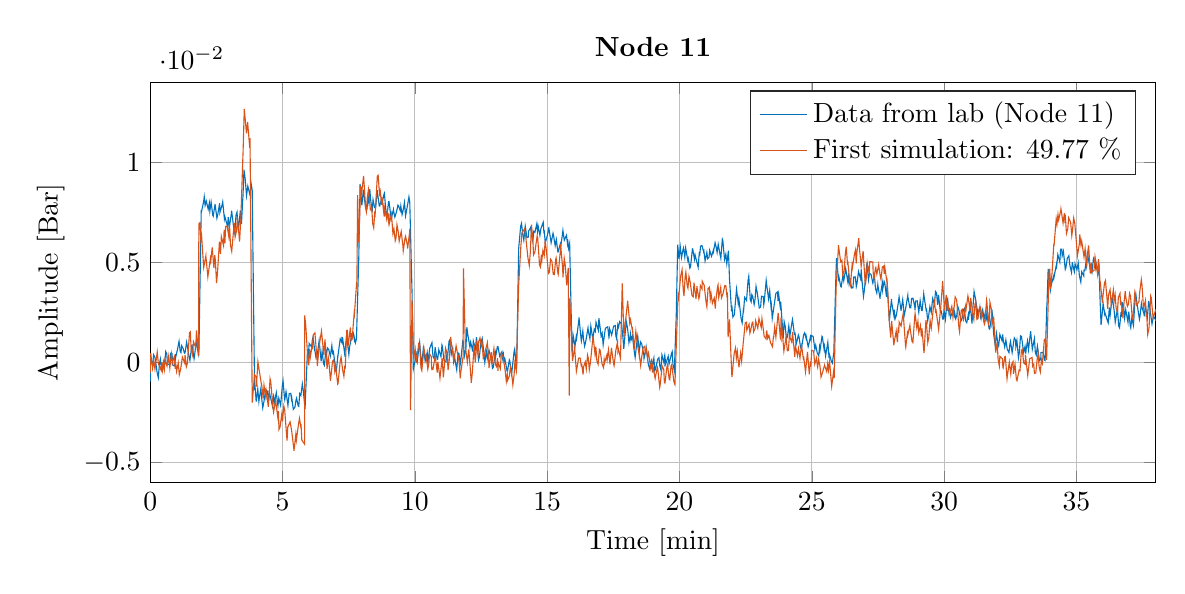
\begin{tikzpicture}

\begin{axis}[%
width=5.028in,
height=2in,
at={(1.011in,0.642in)},
scale only axis,
xmin=0,
xmax=38,
xlabel={Time [min]},
xmajorgrids,
ymin=-0.006,
ymax=0.014,
ylabel={Amplitude [Bar]},
ymajorgrids,
axis background/.style={fill=white},
title style={font=\bfseries},
title={Node 11},
legend style={legend cell align=left,align=left,draw=white!15!black}
]
\addplot [color=mycolor1,solid]
  table[row sep=crcr]{%
0.000833333333333333	-0.00095383988269801\\
0.00916666666666667	0.000151917693059583\\
0.09	-8.47196480935342e-05\\
0.13	0.000384205083089034\\
0.180833333333333	0.000238046725317048\\
0.264166666666667	-0.000527544672531327\\
0.304166666666667	-0.000759832062560556\\
0.350833333333333	-5.2530009775037e-05\\
0.3825	0.000171927468231248\\
0.434166666666667	-0.000395306158357617\\
0.480833333333333	-0.000334406842619622\\
0.519166666666667	0.000117988074292474\\
0.535	-0.000177808602149693\\
0.585833333333333	0.000546893255131881\\
0.626666666666667	0.000421614662755809\\
0.649166666666667	-7.42797653964511e-05\\
0.740833333333333	-0.000104729423265532\\
0.77	0.000461634213097861\\
0.820833333333333	0.000445974389052001\\
0.854166666666667	-0.000138659042036304\\
0.924166666666667	-0.000175198631476498\\
0.964166666666667	0.000420744672534612\\
0.971666666666667	0.000323305767353732\\
1.0325	0.000669561876831926\\
1.08833333333333	0.00106018748777539\\
1.1325	0.00055820312805363\\
1.16166666666667	0.00049295386119258\\
1.18833333333333	0.00083660000000027\\
1.245	0.000691311632451924\\
1.2925	0.000463374193545057\\
1.315	0.00048338396871625\\
1.375	0.00102190791788676\\
1.42	0.000681741739978425\\
1.4675	0.000281546236560404\\
1.49916666666667	0.00010145826001956\\
1.57333333333333	0.00087400957966613\\
1.57916666666667	0.000877489540565463\\
1.6575	0.00018236735092611\\
1.66583333333333	0.000243266666663938\\
1.73333333333333	0.000999288172042562\\
1.755	0.00100102815249098\\
1.81583333333333	0.000417264711623871\\
1.84	0.000611272531764628\\
1.9275	0.00761208387095852\\
1.93666666666667	0.0075459646138761\\
2.015	0.00801923929618911\\
2.04	0.00828632629521028\\
2.07333333333333	0.00785742111436821\\
2.11666666666667	0.00807578866079486\\
2.19	0.00766515327467945\\
2.2325	0.00797747976538976\\
2.25333333333333	0.00757119433039297\\
2.3	0.00802358924730914\\
2.36166666666667	0.00737196656891331\\
2.38	0.00731715718474962\\
2.45166666666667	0.00792963030302407\\
2.4525	0.00789483069403052\\
2.51916666666667	0.00721710830889397\\
2.54	0.00731889716520021\\
2.6225	0.0079609499511179\\
2.63333333333333	0.00750420508308383\\
2.71333333333333	0.00786090107526083\\
2.73916666666667	0.00802793919843273\\
2.80333333333333	0.00716751886607983\\
2.8225	0.00728496754642624\\
2.885	0.0069752510263861\\
2.92166666666667	0.00682735268816476\\
2.94833333333333	0.00726234780058665\\
2.9875	0.00675166353861417\\
3.06583333333333	0.00744156578690183\\
3.075	0.00759381407624393\\
3.15333333333333	0.00673861368524417\\
3.19666666666667	0.0064480369501482\\
3.23916666666667	0.00735456676441618\\
3.27916666666667	0.00752160488758666\\
3.32333333333333	0.00669163421309596\\
3.3475	0.00680908289344306\\
3.405	0.00760860391006307\\
3.4475	0.00693697145649355\\
3.50166666666667	0.00828980625610715\\
3.50333333333333	0.00828545630498215\\
3.5425	0.00963568113391491\\
3.59083333333333	0.00914500664710974\\
3.63833333333333	0.00834461564027511\\
3.6875	0.00881876031280346\\
3.76583333333333	0.00839333509286394\\
3.7675	0.00833939569892625\\
3.81333333333333	0.00894403890517598\\
3.85333333333333	0.00860387272726162\\
3.94166666666667	-0.00118090733138271\\
3.955	-0.0011052181818243\\
4.00416666666667	-0.00195780860215816\\
4.06333333333333	-0.00132358572825805\\
4.10583333333333	-0.00195258866081213\\
4.11916666666667	-0.00181426021506464\\
4.18083333333333	-0.00130444594331602\\
4.205	-0.00171421133921396\\
4.2525	-0.00226839511242499\\
4.29916666666667	-0.00193953880743433\\
4.36166666666667	-0.00135229540566112\\
4.42916666666667	-0.00143581446724991\\
4.46083333333333	-0.0018542797654035\\
4.47833333333333	-0.00186558963831654\\
4.5025	-0.00148540391007113\\
4.61583333333333	-0.00216573626587999\\
4.64	-0.00173596109480623\\
4.65916666666667	-0.00165853196480295\\
4.68583333333333	-0.00203262776147706\\
4.76416666666667	-0.00150454369501457\\
4.81666666666667	-0.00210222697947696\\
4.825	-0.00216921622679248\\
4.85916666666667	-0.00178294056697009\\
4.9275	-0.00213963655913996\\
4.99083333333333	-0.00116698748777819\\
5.01833333333333	-0.000914690322571188\\
5.07416666666667	-0.00178903049853996\\
5.08333333333333	-0.00185862971651996\\
5.13083333333333	-0.00146017419353367\\
5.20333333333333	-0.00214398651025502\\
5.25083333333333	-0.00156109305962954\\
5.31083333333333	-0.00154282326491992\\
5.33916666666667	-0.00183253000978137\\
5.34916666666667	-0.0017768506353931\\
5.40583333333333	-0.00234321427174816\\
5.46666666666667	-0.00223794545453582\\
5.51	-0.0018734195503384\\
5.53	-0.00178381055719254\\
5.59333333333333	-0.00217878611926489\\
5.61333333333333	-0.00219444594330437\\
5.64833333333333	-0.0015576130987156\\
5.6925	-0.00164635210164615\\
5.7475	-0.00107302854349167\\
5.7825	-0.0013975348973673\\
5.85	-0.00232842443793113\\
5.8675	-0.00171421133920258\\
5.93416666666667	0.00034244555229182\\
5.9675	0.000240656695986302\\
6.00583333333333	0.000950568719447681\\
6.095	0.000782660606056168\\
6.13	0.00116197634407772\\
6.15333333333333	0.00127159511240368\\
6.21583333333333	0.000585172825033481\\
6.2175	0.000636502248296755\\
6.26666666666667	0.00022760684262127\\
6.3175	0.000429444574776061\\
6.38166666666667	0.00109237712610058\\
6.395	0.000916639100681543\\
6.45833333333333	6.40486803462625e-05\\
6.49333333333333	0.000558203128052576\\
6.55	-6.12299120248405e-05\\
6.5775	-0.00014300899316308\\
6.63666666666667	0.0005590731182821\\
6.65833333333333	0.000384205083088368\\
6.6975	0.000726111241434096\\
6.74333333333333	0.000659121994131373\\
6.80416666666667	0.000313735874873128\\
6.8625	0.000846169892460613\\
6.88916666666667	0.000466854154429125\\
6.91916666666667	0.000544283284445196\\
7.00583333333333	-0.000256107722388738\\
7.03583333333333	-0.000403136070390497\\
7.09166666666667	0.00038768504397671\\
7.09416666666667	0.000345925513187267\\
7.17833333333333	0.00117763616814134\\
7.24166666666667	0.00099406823069903\\
7.24666666666667	0.00124984535680003\\
7.26833333333333	0.00123766549364607\\
7.34666666666667	0.000441624437922922\\
7.3575	0.000521663538607747\\
7.41916666666667	0.00132205454545589\\
7.44333333333333	0.00108628719452786\\
7.50583333333333	0.00040160488757271\\
7.53083333333333	0.000740031085037202\\
7.61666666666667	0.00143863323559404\\
7.66916666666667	0.00149779257088486\\
7.705	0.00119677595308479\\
7.71083333333333	0.00126028523948921\\
7.7525	0.000982758357777447\\
7.79333333333333	0.00118111612905242\\
7.88166666666667	0.00530051984360685\\
7.92916666666667	0.00893011906158284\\
7.9975	0.0078539411534877\\
8.055	0.00864476226782931\\
8.05666666666667	0.00859169286411832\\
8.13916666666667	0.00772344261978622\\
8.19333333333333	0.00768951300100587\\
8.22833333333333	0.00836723538612039\\
8.255	0.00807752864124045\\
8.29833333333333	0.00866042209188725\\
8.32333333333333	0.00820715718478485\\
8.385	0.00753639472142145\\
8.42	0.00813929794722984\\
8.47916666666667	0.0077538922776427\\
8.52	0.00777303206256197\\
8.57666666666667	0.0086134426197646\\
8.58166666666667	0.00853601348975136\\
8.65583333333333	0.00782349149561415\\
8.67083333333333	0.00782523147606473\\
8.73333333333333	0.00814973782993325\\
8.76416666666667	0.00799487956989256\\
8.84416666666667	0.00846815425222761\\
8.84833333333333	0.00847772414470574\\
8.91916666666667	0.00735804672531518\\
8.94	0.00728148758551303\\
9.00666666666667	0.00803837908113966\\
9.02333333333333	0.0080453390029476\\
9.10666666666667	0.00716838885629731\\
9.19	0.00764862346041473\\
9.195	0.00757902424242904\\
9.24333333333333	0.00727104770282669\\
9.30166666666667	0.00751029501463168\\
9.36083333333333	0.00787047096773966\\
9.38083333333333	0.00784263128054197\\
9.44833333333333	0.00759207409578838\\
9.46916666666667	0.00782697145651529\\
9.51666666666667	0.0073919763441069\\
9.54916666666667	0.00755553450637197\\
9.6075	0.00800009951124142\\
9.64833333333333	0.00733194701857659\\
9.72	0.00784089130009993\\
9.77583333333333	0.0082837163244989\\
9.8075	0.00799922952100476\\
9.895	0.00339872121211049\\
9.94083333333333	-0.000345716715551669\\
10.0208333333333	0.000158007624622813\\
10.0383333333333	0.000559073118245157\\
10.0916666666667	6.14387096704028e-05\\
10.15	0.000716541348984412\\
10.18	0.00100102815248423\\
10.2433333333333	1.09792766494754e-05\\
10.2633333333333	-8.3849657838142e-05\\
10.3266666666667	0.000821810166186793\\
10.3333333333333	0.00067826177908617\\
10.3883333333333	7.62285434888488e-05\\
10.4658333333333	0.000499913782999822\\
10.4916666666667	-7.601974583335e-05\\
10.51	0.000221516911057096\\
10.5666666666667	0.00073916109482472\\
10.6458333333333	0.000992328250225716\\
10.6833333333333	0.000311995894406919\\
10.7283333333333	0.000194547214061952\\
10.7675	0.000760910850451102\\
10.7708333333333	0.000695661583588997\\
10.8441666666667	0.000160617595278773\\
10.8641666666667	0.000175407429105739\\
10.9033333333333	0.000643462170046433\\
10.9866666666667	0.000291116129025715\\
11.0233333333333	0.000871399608993823\\
11.0391666666667	0.000807020332351305\\
11.1016666666667	8.40584555192314e-05\\
11.1758333333333	2.92490713548477e-05\\
11.2083333333333	0.000408564809376372\\
11.2325	0.000251096578682608\\
11.2908333333333	0.00106105747800886\\
11.3158333333333	0.00112108680352496\\
11.3741666666667	0.000403344868027539\\
11.4308333333333	0.00072176129030202\\
11.4658333333333	4.31689149451575e-05\\
11.4991666666667	0.000297206060571431\\
11.5408333333333	-6.12299120546778e-05\\
11.5816666666667	-0.000365726490724638\\
11.6333333333333	0.000474684066466613\\
11.6641666666667	0.000451194330403887\\
11.7166666666667	-6.81898338427411e-05\\
11.735	9.18883675354032e-05\\
11.8108333333333	0.00108802717495851\\
11.8291666666667	0.00105061759529979\\
11.8716666666667	0.00031721583576716\\
11.9275	0.000671301857292445\\
11.965	0.00176400957966796\\
11.9966666666667	0.00141862346037275\\
12.0816666666667	0.000767870772216434\\
12.1083333333333	0.00101581798627709\\
12.1691666666667	0.000662601955031095\\
12.18	0.000546893255145203\\
12.2091666666667	0.001072367350929\\
12.29	0.000690441642225925\\
12.3283333333333	0.00126376520042018\\
12.355	0.000929688954076413\\
12.4033333333333	0.00012059804496406\\
12.4366666666667	0.000258926490684569\\
12.4891666666667	0.000950568719426365\\
12.5441666666667	0.00120808582597368\\
12.6091666666667	0.000486863929612058\\
12.6433333333333	4.88934505260552e-06\\
12.6966666666667	0.000550373216017919\\
12.7016666666667	0.000574732942314471\\
12.7366666666667	0.000198897165199746\\
12.8008333333333	0.000618232453555884\\
12.8716666666667	0.000221516911017294\\
12.8775	0.000354625415417364\\
12.9325	-0.000291777321623915\\
12.96	-0.000255237732179087\\
13.04	0.000447714369482849\\
13.05	0.000280676246319472\\
13.1183333333333	0.000800930400774336\\
13.1391666666667	0.000797450439870367\\
13.2066666666667	0.000308515933525683\\
13.2908333333333	0.000537323362652886\\
13.3083333333333	0.000194547214053431\\
13.345	0.000421614662730052\\
13.3741666666667	6.31786900953946e-05\\
13.4016666666667	0.000178887390009708\\
13.485	-0.000433585728254082\\
13.4991666666667	-0.000446635581630467\\
13.57	0.000136257869004952\\
13.585	9.97182795516027e-05\\
13.6533333333333	-0.000565824242423185\\
13.6675	-0.000444025610948945\\
13.7466666666667	0.000523403519034155\\
13.7725	0.000668691886608064\\
13.835	-0.000247407820120282\\
13.8458333333333	-0.000255237732159186\\
13.9225	0.00569549540567496\\
13.9966666666667	0.00680473294231948\\
14.03	0.00695785122186696\\
14.0816666666667	0.00635842795697389\\
14.1166666666667	0.00611309071358054\\
14.1708333333333	0.00682039276639448\\
14.185	0.00670207409580431\\
14.2325	0.00624532922776955\\
14.2858333333333	0.00626794897361552\\
14.3	0.00657331554252782\\
14.3758333333333	0.00675688347996586\\
14.4366666666667	0.00610178084068028\\
14.4558333333333	0.00605828132945024\\
14.4941666666667	0.00656809560117327\\
14.5358333333333	0.00651067624629323\\
14.6091666666667	0.00694132140764059\\
14.6341666666667	0.00655591573804207\\
14.6591666666667	0.00680995288368255\\
14.725	0.006354078005856\\
14.7625	0.00669163421312366\\
14.85	0.00701266060604558\\
14.8783333333333	0.00646021681327799\\
14.8883333333333	0.00660289521014482\\
14.9275	0.0059791122189751\\
15.0175	0.00641062737046813\\
15.0608333333333	0.00673687370476447\\
15.0616666666667	0.00673774369498975\\
15.1483333333333	0.005989552101687\\
15.2216666666667	0.00646282678397941\\
15.2383333333333	0.00636625786900996\\
15.3025	0.00583817380251336\\
15.3458333333333	0.00614963030301116\\
15.4041666666667	0.00552758729227779\\
15.4175	0.00552845728251444\\
15.4891666666667	0.00589820312807493\\
15.505	0.00573464496579848\\
15.5841666666667	0.0064810965786791\\
15.595	0.00660289521016755\\
15.6458333333333	0.00611657067450441\\
15.7283333333333	0.00635755796669746\\
15.7616666666667	0.00600173196481255\\
15.7716666666667	0.00617051006842079\\
15.8125	0.00569897536653347\\
15.8491666666667	0.00594779257080522\\
15.9366666666667	0.000632152297163235\\
15.945	0.000493823851428515\\
15.9808333333333	0.00135337419355328\\
16.0508333333333	0.000810500293255273\\
16.0975	0.00129508484842522\\
16.1116666666667	0.00120808582596513\\
16.1991666666667	0.00215724516131677\\
16.2025	0.00225120410559046\\
16.2858333333333	0.00110977693057071\\
16.2908333333333	0.00106801739978554\\
16.3466666666667	0.00157174173992305\\
16.3741666666667	0.0011480565004604\\
16.415	0.000813110263908401\\
16.4616666666667	0.00108802717495568\\
16.5425	0.00173007996082791\\
16.5566666666667	0.00156913176923584\\
16.615	0.0011872060605356\\
16.65	0.00181881896380109\\
16.7083333333333	0.00128638494624059\\
16.7325	0.00126115522973583\\
16.7783333333333	0.00166048074290193\\
16.8175	0.00155173196476999\\
16.8441666666667	0.00201456676442152\\
16.9325	0.00161263128053979\\
16.9541666666667	0.00221466451606606\\
16.9908333333333	0.00185274858254164\\
17.0375	0.00132118455520075\\
17.0766666666667	0.00146647292276048\\
17.115	0.00089053939390174\\
17.1625	0.00136294408598592\\
17.1991666666667	0.00171355014659871\\
17.2875	0.00178227937444153\\
17.3366666666667	0.00123418553279184\\
17.3383333333333	0.00123853548391256\\
17.3591666666667	0.00168919042034762\\
17.4366666666667	0.00137338396871203\\
17.5116666666667	0.00181794897357013\\
17.5716666666667	0.00184317869013176\\
17.595	0.00132205454543172\\
17.6191666666667	0.00120634584552595\\
17.6683333333333	0.0018858082111706\\
17.6975	0.00175791964812225\\
17.7358333333333	0.0020415364614394\\
17.8116666666667	0.001922347800587\\
17.8608333333333	0.00126202521994973\\
17.8941666666667	0.00067826177908617\\
17.95	0.0015099724339962\\
17.9933333333333	0.00201630674484934\\
18.0383333333333	0.00170833020525268\\
18.09	0.000993198240445331\\
18.1491666666667	0.00143776324532044\\
18.1675	0.00110716695990054\\
18.22	0.00132988445751042\\
18.2966666666667	0.000485123949187066\\
18.3241666666667	0.000254576539595097\\
18.3766666666667	0.000867919648061433\\
18.4216666666667	0.00131248465294223\\
18.4716666666667	0.000639112218982552\\
18.4816666666667	0.000579952883686063\\
18.5283333333333	0.0010288678396535\\
18.5708333333333	0.000937518866055642\\
18.6508333333333	0.000383335092846021\\
18.6591666666667	0.000198027174940357\\
18.7383333333333	0.000712191397843787\\
18.7408333333333	0.00074438103617358\\
18.8233333333333	-0.000109079374419674\\
18.8725	-0.000315267057646867\\
18.9133333333333	1.96791789108253e-05\\
18.9358333333333	0.000111898142705541\\
18.985	-0.000127349169167651\\
19.0316666666667	0.000215426979417593\\
19.0658333333333	-0.000415315933525978\\
19.0966666666667	-0.000317877028351149\\
19.175	0.000164967546419398\\
19.2233333333333	0.000245006647139723\\
19.2558333333333	-0.00017606862169825\\
19.2966666666667	-0.000363986510325237\\
19.3366666666667	0.000378115151437486\\
19.4208333333333	-5.25300097933279e-05\\
19.4383333333333	0.000325915738011467\\
19.4441666666667	0.000363325317675883\\
19.4783333333333	-8.12396871878729e-05\\
19.5725	0.000313735874857501\\
19.6041666666667	-7.86297165404626e-05\\
19.6133333333333	-3.42602150623927e-05\\
19.6975	0.000445104398852481\\
19.7241666666667	0.000539933333323056\\
19.7525	-9.42895405671162e-05\\
19.8058333333333	-0.000406616031250417\\
19.8766666666667	0.00231906334311138\\
19.9325	0.00588602326492951\\
19.9791666666667	0.00517263128053291\\
20.0291666666667	0.00578336441837454\\
20.075	0.00524136050829616\\
20.1325	0.00564242600194123\\
20.1525	0.00572768504396212\\
20.2008333333333	0.00527268015637222\\
20.2316666666667	0.00571985513194026\\
20.3141666666667	0.00510303206247617\\
20.3316666666667	0.00519699100676124\\
20.3908333333333	0.00471762639293163\\
20.4158333333333	0.00476982580642019\\
20.4883333333333	0.00568418553273778\\
20.4991666666667	0.00568244555228151\\
20.565	0.0051569714564437\\
20.59	0.00537446901266211\\
20.6625	0.00498645337245879\\
20.705	0.00476025591393639\\
20.7508333333333	0.00554063714561726\\
20.7641666666667	0.00535010928639967\\
20.795	0.00581990400780233\\
20.8491666666667	0.00584600371451532\\
20.9208333333333	0.00548669775168381\\
20.9266666666667	0.00552410733134825\\
20.9666666666667	0.00507780234596569\\
21.0333333333333	0.00550496754640908\\
21.0625	0.00518742111440251\\
21.1141666666667	0.0052578903225822\\
21.1408333333333	0.00560936637342596\\
21.2091666666667	0.00530834975562589\\
21.2758333333333	0.00559979648090805\\
21.2825	0.00554585708697464\\
21.345	0.00598520215052081\\
21.385	0.00577379452586801\\
21.4208333333333	0.00550235757571618\\
21.4633333333333	0.00590255307917009\\
21.5358333333333	0.00537620899312974\\
21.5616666666667	0.00520917087002321\\
21.6183333333333	0.00616790009777904\\
21.6366666666667	0.00611657067448737\\
21.7016666666667	0.00514827155422498\\
21.7508333333333	0.00541535855323905\\
21.7875	0.00494382385140288\\
21.8491666666667	0.00559109657864956\\
21.89	0.00415909266857856\\
21.9625	0.00266357947209034\\
21.9841666666667	0.00274535855321578\\
22.0166666666667	0.00227121388072651\\
22.0725	0.00239040254152204\\
22.1525	0.00362230869978367\\
22.1558333333333	0.00366667820125602\\
22.22	0.00293762639292941\\
22.2441666666667	0.00317078377319152\\
22.3283333333333	0.00219204477029397\\
22.3675	0.00197976715549547\\
22.4133333333333	0.00263486979477537\\
22.4233333333333	0.0026052901271385\\
22.4608333333333	0.00325082287390618\\
22.5333333333333	0.00309944457472403\\
22.5891666666667	0.00408862346039887\\
22.6175	0.00430612101664568\\
22.6758333333333	0.00313076422285694\\
22.7083333333333	0.00302810537628492\\
22.7333333333333	0.00339176129028265\\
22.7683333333333	0.00329519237533307\\
22.8208333333333	0.002899346823034\\
22.8566666666667	0.00317774369498242\\
22.8916666666667	0.00380239667641721\\
22.9416666666667	0.00346397047890723\\
23.0141666666667	0.0027253487780968\\
23.065	0.00277406823070128\\
23.0966666666667	0.0033143321603632\\
23.1625	0.00329780234601462\\
23.185	0.00289151691100645\\
23.2033333333333	0.00304289521011472\\
23.2758333333333	0.00410602326493295\\
23.2941666666667	0.00390244555230201\\
23.3658333333333	0.00318122365590059\\
23.4083333333333	0.00358924907134228\\
23.4566666666667	0.00281147781037139\\
23.4691666666667	0.00289673685239225\\
23.505	0.0022129245356837\\
23.5591666666667	0.00270359902247042\\
23.6416666666667	0.0034578805473473\\
23.7033333333333	0.003525739784908\\
23.7241666666667	0.00307160488755476\\
23.7508333333333	0.00337871143694318\\
23.8025	0.00281669775172877\\
23.8233333333333	0.00303680527858891\\
23.9025	0.00156652179854863\\
23.9258333333333	0.00137338396863246\\
23.955	0.00204153646132002\\
23.9925	0.00183708875855476\\
24.0408333333333	0.00119155601171886\\
24.0808333333333	0.00128203499511417\\
24.13	0.00182316891497866\\
24.1733333333333	0.00135250420333935\\
24.2541666666667	0.00203892649072376\\
24.27	0.00214941524923806\\
24.3416666666667	0.00142384340170457\\
24.3683333333333	0.00145081309867126\\
24.4091666666667	0.00091837908109374\\
24.4375	0.00106105747801169\\
24.4916666666667	0.00137164398830694\\
24.5166666666667	0.00128377497560453\\
24.5775	0.000733071163239202\\
24.615	0.000750470967756239\\
24.6891666666667	0.00137773391983279\\
24.7283333333333	0.00148126275659027\\
24.7775	0.00123070557186228\\
24.7858333333333	0.00131248465300476\\
24.8633333333333	0.000783530596288579\\
24.8683333333333	0.000802670381244791\\
24.9475	0.00127942502449518\\
24.9691666666667	0.00114979648095645\\
24.9816666666667	0.00135337419351916\\
25.0508333333333	0.0013037847507292\\
25.1141666666667	0.000667821896354365\\
25.1475	0.000864439687188717\\
25.2083333333333	0.000462504203301295\\
25.2616666666667	0.000332875659830784\\
25.2925	0.000778310654965281\\
25.3108333333333	0.000614752492680309\\
25.385	0.00130900469207521\\
25.4008333333333	0.00127594506351447\\
25.4633333333333	0.000670431867035887\\
25.48	0.000805280351914961\\
25.5208333333333	0.000327655718456332\\
25.605	0.00100711808407827\\
25.6533333333333	0.000210207038145477\\
25.665	0.000400734897380101\\
25.7416666666667	5.01288367047714e-05\\
25.7766666666667	-3.25202346231901e-05\\
25.8283333333333	0.000482513978499854\\
25.83	0.000435534506357305\\
25.9175	0.00467586686218627\\
25.935	0.00521352082110985\\
26.005	0.00417475249266208\\
26.025	0.00427480136854119\\
26.0883333333333	0.00381892649074875\\
26.1091666666667	0.00377977693063375\\
26.1758333333333	0.00436006041047679\\
26.2075	0.00409558338212723\\
26.2675	0.00456102815246598\\
26.2808333333333	0.00469500664707997\\
26.3558333333333	0.00406513372433895\\
26.3833333333333	0.00431743088950046\\
26.4108333333333	0.00390505552294376\\
26.45	0.00411298318667835\\
26.5033333333333	0.00372322756593921\\
26.5533333333333	0.00373366744868808\\
26.5866666666667	0.00427741133919429\\
26.6433333333333	0.00427480136854119\\
26.6808333333333	0.00379543675464336\\
26.7066666666667	0.00393985513196643\\
26.7633333333333	0.00454536832849617\\
26.8466666666667	0.0041756224828419\\
26.8683333333333	0.00465324711627207\\
26.8825	0.00430873098727039\\
26.9516666666667	0.00330563225804217\\
26.9866666666667	0.00362230869990302\\
27.0558333333333	0.00460365767349916\\
27.0833333333333	0.00498297341154061\\
27.1408333333333	0.0041312529814434\\
27.1433333333333	0.00415387272728371\\
27.18	0.0044574993157028\\
27.2375	0.00440442991197759\\
27.3041666666667	0.0039824846529655\\
27.3666666666667	0.00433744066468197\\
27.4058333333333	0.00370060782009321\\
27.4541666666667	0.00347702033228078\\
27.4925	0.00388678572824122\\
27.4933333333333	0.00387373587487336\\
27.5791666666667	0.00318818357771991\\
27.5816666666667	0.00328997243402118\\
27.6633333333333	0.00396508484853375\\
27.6741666666667	0.00363622854353599\\
27.7316666666667	0.00405904379273356\\
27.7575	0.00397378475073543\\
27.8208333333333	0.00328040254159423\\
27.8475	0.00394507507336361\\
27.9283333333333	0.00209634584549012\\
27.9316666666667	0.00209895581617164\\
28.0116666666667	0.00317687370477987\\
28.0191666666667	0.00299591573801766\\
28.0991666666667	0.00237039276634055\\
28.1133333333333	0.00264356969694293\\
28.1475	0.00217986490713432\\
28.1958333333333	0.00236604281519706\\
28.28	0.00309596461389677\\
28.2975	0.00327953255135188\\
28.3691666666667	0.00261746999025267\\
28.37	0.00258963030305498\\
28.435	0.00314642404696319\\
28.46	0.00282365767356513\\
28.4858333333333	0.00232254330402387\\
28.5441666666667	0.00268967917884314\\
28.6275	0.00335870166176169\\
28.6316666666667	0.00327431260996039\\
28.7041666666667	0.00273926862170701\\
28.7391666666667	0.00273578866080587\\
28.7708333333333	0.00319949345063156\\
28.8233333333333	0.00321515327472643\\
28.895	0.00274535855324989\\
28.9008333333333	0.00262355992177279\\
28.9216666666667	0.00307073489734083\\
28.9833333333333	0.00308378475072008\\
29.0425	0.0025165511241369\\
29.0941666666667	0.00309248465301271\\
29.1458333333333	0.00260181016616348\\
29.17	0.00259572023459786\\
29.2291666666667	0.00343961075270163\\
29.245	0.0032777925708786\\
29.3283333333333	0.00254613079175106\\
29.3325	0.00269750909088207\\
29.3791666666667	0.00208764594326571\\
29.4208333333333	0.00239823245353254\\
29.4616666666667	0.0027905980449589\\
29.5116666666667	0.00250350127074062\\
29.5675	0.00320384340172955\\
29.6325	0.00290021681329908\\
29.6741666666667	0.00355096950140141\\
29.7133333333333	0.00347702033230352\\
29.7541666666667	0.00288368699898459\\
29.7883333333333	0.00337784144668948\\
29.855	0.00255483069400389\\
29.8958333333333	0.00257136050826151\\
29.9425	0.00217638494622752\\
29.9733333333333	0.00217290498534911\\
29.995	0.00263312981431343\\
30.0491666666667	0.00216072512222926\\
30.1166666666667	0.003112494428126\\
30.1325	0.00317600371450913\\
30.1816666666667	0.00246435171067677\\
30.21	0.00261833998048933\\
30.24	0.00225207409581576\\
30.3458333333333	0.00265748954055314\\
30.3816666666667	0.00237474271747265\\
30.3958333333333	0.00250524125118548\\
30.4375	0.00218943479958403\\
30.4758333333333	0.00232602326486248\\
30.515	0.00280973782982988\\
30.56	0.00260790009767223\\
30.6358333333333	0.00207807605082738\\
30.6791666666667	0.00220770459428654\\
30.7266666666667	0.00263312981425093\\
30.7625	0.0027018590420369\\
30.8141666666667	0.0020754660802027\\
30.8558333333333	0.00199455698929119\\
30.9066666666667	0.00235212297161527\\
30.9133333333333	0.00213462541542531\\
30.9941666666667	0.00284105747795141\\
30.9958333333333	0.00279494799603416\\
31.0525	0.0019440975561395\\
31.0833333333333	0.00263921974577105\\
31.1308333333333	0.00355009951113064\\
31.1758333333333	0.00324647292273997\\
31.2583333333333	0.00257484046917969\\
31.2683333333333	0.00239562248290784\\
31.3458333333333	0.00271838885629452\\
31.3491666666667	0.00274709853371183\\
31.3741666666667	0.00226599393936913\\
31.4558333333333	0.00264095972628983\\
31.5125	0.00217725493646984\\
31.5541666666667	0.00249045141742391\\
31.5825	0.00205458631474476\\
31.6125	0.00246000175946509\\
31.695	0.00171616011738823\\
31.7225	0.0016717906159045\\
31.7841666666667	0.00224859413492032\\
31.8083333333333	0.00264617966766426\\
31.8716666666667	0.00142384340178414\\
31.9308333333333	0.000842689931579377\\
31.9758333333333	0.00145429305953829\\
32.0308333333333	0.000947088758545128\\
32.0608333333333	0.000829640078194444\\
32.105	0.00140209364619184\\
32.1875	0.00108976715562795\\
32.2141666666667	0.00140644359746037\\
32.2275	0.00117763616826214\\
32.2891666666667	0.000768740762481485\\
32.3333333333333	0.00112108680359033\\
32.3841666666667	0.000672171847594466\\
32.45	0.000492953861106621\\
32.4841666666667	0.000902719257061368\\
32.5075	0.0010514875855677\\
32.5691666666667	0.000499043792768855\\
32.5725	0.000527753470197512\\
32.6508333333333	0.00122722561091568\\
32.6983333333333	0.0011158668621363\\
32.71	0.000797450439841946\\
32.75	0.00109498709674088\\
32.8091666666667	0.000236306744881204\\
32.84	0.00048338396869102\\
32.8866666666667	0.001331624437961\\
32.9233333333333	0.00130030478983945\\
33.0058333333333	0.000499043792700632\\
33.0558333333333	0.000796580449656442\\
33.0858333333333	0.00044945435005847\\
33.0975	0.000645202150616392\\
33.1508333333333	0.0010767173020611\\
33.1883333333333	0.000642592179877999\\
33.2691666666667	0.00156913176918469\\
33.2725	0.00150823245342627\\
33.3316666666667	0.000665211925655773\\
33.4116666666667	0.00119242600196121\\
33.4466666666667	0.000496433822144177\\
33.4816666666667	0.000374635190650036\\
33.525	0.000818330205351048\\
33.535	0.000725241251262831\\
33.6025	9.10183773215056e-05\\
33.6516666666667	0.000162357575862915\\
33.6583333333333	0.00049121388086068\\
33.7341666666667	0.000511223655934173\\
33.7908333333333	0.000124078005723088\\
33.8158333333333	9.62383185936222e-05\\
33.8816666666667	0.00287933704792639\\
33.8858333333333	0.00286715718481792\\
33.9308333333333	0.00467760684275054\\
34.0141666666667	0.00361708875857975\\
34.06	0.0040216342129327\\
34.0658333333333	0.00396334486787855\\
34.145	0.00435484046933543\\
34.1516666666667	0.00425827155436881\\
34.2358333333333	0.00484899491695504\\
34.24	0.00466890694042948\\
34.2966666666667	0.00539534877812575\\
34.3716666666667	0.00502821290322689\\
34.4	0.00566330576741056\\
34.4458333333333	0.00566939569902733\\
34.4608333333333	0.00532574956021681\\
34.5083333333333	0.00555977693069853\\
34.5775	0.00465672707724143\\
34.6	0.00473502619744867\\
34.6541666666667	0.00520656089930188\\
34.7141666666667	0.00533705943284421\\
34.75	0.00486639472129016\\
34.8125	0.00450795874891699\\
34.8458333333333	0.00501255307929685\\
34.8483333333333	0.00496296363648416\\
34.9191666666667	0.00454101837730722\\
34.9475	0.00493686392957787\\
35.0175	0.00464367722383377\\
35.0675	0.00498036344086475\\
35.1108333333333	0.00434266060607916\\
35.165	0.00401902424248993\\
35.1983333333333	0.00453666842616376\\
35.2766666666667	0.00432874076234957\\
35.2858333333333	0.00461583753652239\\
35.3216666666667	0.00461322756576127\\
35.36	0.00501690303016747\\
35.3783333333333	0.00484725493641353\\
35.4108333333333	0.00546842795696992\\
35.4658333333333	0.00508302228737992\\
35.5191666666667	0.00466455698925192\\
35.585	0.00447489912007204\\
35.6366666666667	0.0051421816225741\\
35.6558333333333	0.00522222072330014\\
35.7208333333333	0.00475416598233669\\
35.7291666666667	0.00504213274676321\\
35.8075	0.00448968895405533\\
35.8475	0.00500994310855848\\
35.8991666666667	0.00287411710651786\\
35.9	0.00289151691101214\\
35.93	0.00188058826979048\\
36.0083333333333	0.00294197634415813\\
36.065	0.00243912199419474\\
36.0741666666667	0.00249654134908614\\
36.1583333333333	0.00213636539589859\\
36.2	0.00197976715540452\\
36.2425	0.0027549284457962\\
36.2725	0.00236169286410476\\
36.3075	0.00277232825016543\\
36.3583333333333	0.00322472316716474\\
36.4241666666667	0.00259833020524528\\
36.4658333333333	0.00201804672529424\\
36.5483333333333	0.00267314936447183\\
36.5975	0.00182316891492182\\
36.6283333333333	0.00173616989248448\\
36.6866666666667	0.0025235110458596\\
36.6916666666667	0.00228513372425712\\
36.7458333333333	0.0029532862170584\\
36.775	0.00288629696978551\\
36.8216666666667	0.00221292453568939\\
36.8625	0.00264008973610433\\
36.9475	0.00201195679377977\\
36.9766666666667	0.00254265083096361\\
37.0358333333333	0.00181185904203293\\
37.0516666666667	0.0017335599217802\\
37.0916666666667	0.00221031456495102\\
37.1541666666667	0.00185448856310022\\
37.2125	0.00313163421317886\\
37.2441666666667	0.00342482091879792\\
37.2983333333333	0.00284714740964209\\
37.3	0.00284888739010403\\
37.3808333333333	0.00215898514171048\\
37.3966666666667	0.00226860391006203\\
37.4541666666667	0.00294458631480557\\
37.475	0.00276797829912429\\
37.5625	0.0023790926686218\\
37.5641666666667	0.00230949345063328\\
37.6025	0.00285323734119064\\
37.6825	0.00225555405666572\\
37.7266666666667	0.00304637517106701\\
37.7375	0.003040285239473\\
37.825	0.00221553450632545\\
37.855	0.00192756774194439\\
37.9125	0.00233124320636197\\
38	0.0020885159335933\\
};
\addlegendentry{Data from lab (Node 11)};

\addplot [color=mycolor2,solid]
  table[row sep=crcr]{%
0.000833333333333333	-0.000211127965843747\\
0.00166666666666667	-0.000508341394804168\\
0.0175	0.000472919771457708\\
0.0891666666666667	-0.000293478767521926\\
0.135	9.91617723337173e-05\\
0.178333333333333	-0.000336050733193557\\
0.264166666666667	0.000524602051073829\\
0.305833333333333	-5.10669842976259e-05\\
0.410833333333333	-0.000387652567747461\\
0.4275	1.83342118447849e-05\\
0.4625	-0.000369477031193901\\
0.493333333333333	1.83681418376112e-05\\
0.533333333333333	-0.000347013390213956\\
0.558333333333333	0.000145715538105509\\
0.634166666666667	-0.000182302491131082\\
0.695833333333333	0.000321255528192011\\
0.701666666666667	0.000224690955736758\\
0.74	-0.000275487426181832\\
0.8025	0.000399548403263137\\
0.831666666666667	-2.6958968550483e-05\\
0.908333333333333	0.000293855886279247\\
0.945	-0.000312509224501555\\
0.965	-4.23668359344008e-05\\
0.995833333333333	-0.000446061761506679\\
1.05916666666667	-2.20730424066132e-05\\
1.0975	-0.000608818481801867\\
1.14583333333333	-0.000352276622048663\\
1.215	0.000267733163070793\\
1.30333333333333	-2.93325025400322e-05\\
1.315	0.000335891542652396\\
1.31583333333333	0.000372701611737473\\
1.36416666666667	-0.00021160702285355\\
1.4025	-4.58089326215178e-05\\
1.485	0.00149404626274318\\
1.5125	0.00152957631607052\\
1.5475	0.000639145005131954\\
1.60166666666667	0.000360385738304194\\
1.63333333333333	0.00104008602600728\\
1.71833333333333	0.000746918609294653\\
1.74833333333333	0.00160433793900474\\
1.83166666666667	0.000323845981810013\\
1.83583333333333	0.00692732937977012\\
1.8775	0.00698749507666718\\
1.91	0.00615043228281446\\
1.93916666666667	0.00636347021262969\\
2.0125	0.00490500672595164\\
2.02166666666667	0.00475308253772229\\
2.10166666666667	0.00533008415356738\\
2.1025	0.00530527275794402\\
2.1775	0.00428347595345755\\
2.19	0.00440331001586843\\
2.2725	0.00520159353553618\\
2.28833333333333	0.00507060834538991\\
2.34083333333333	0.00575850886753942\\
2.40666666666667	0.00472554983941665\\
2.43916666666667	0.0053622096385424\\
2.46083333333333	0.00509992144944089\\
2.50583333333333	0.003974666526096\\
2.54416666666667	0.00453670316705768\\
2.61416666666667	0.00604019747695315\\
2.65583333333333	0.00543225888621698\\
2.68666666666667	0.00630624605001899\\
2.76916666666667	0.00584652175735414\\
2.7925	0.00662651224484031\\
2.82166666666667	0.00596353111342065\\
2.85	0.00679993353515654\\
2.90416666666667	0.00683175926370654\\
2.96916666666667	0.00629587510919386\\
2.995	0.00691650990476591\\
3.03333333333333	0.00585057977675543\\
3.07916666666667	0.00556017934441743\\
3.1525	0.00665840185736491\\
3.19	0.00696150409144547\\
3.20916666666667	0.00628767796482195\\
3.2625	0.00658789328829117\\
3.29333333333333	0.00726364778266138\\
3.37666666666667	0.0060512647780534\\
3.415	0.0070131682813213\\
3.41833333333333	0.00696906915441109\\
3.50333333333333	0.0103762332177025\\
3.50416666666667	0.010339381125089\\
3.55333333333333	0.0126742693257365\\
3.63666666666667	0.0114618271915086\\
3.67833333333333	0.0119835822942229\\
3.67916666666667	0.012034648510795\\
3.76	0.0107318755366993\\
3.77083333333333	0.0112150257736402\\
3.85333333333333	-0.00192045080971089\\
3.85666666666667	-0.00200231392671077\\
3.94	-0.000606768062447195\\
3.99333333333333	-0.00070815556390615\\
4.0225	-0.00120215982804163\\
4.02916666666667	-0.000829728777493028\\
4.06916666666667	3.77576783002166e-05\\
4.11833333333333	-0.00039455292476545\\
4.20166666666667	-0.0010955928836283\\
4.20416666666667	-0.001020936002203\\
4.2675	-0.00180661175531781\\
4.29916666666667	-0.00114134984396942\\
4.36333333333333	-0.00169756470250582\\
4.37916666666667	-0.00140525820391562\\
4.4625	-0.00221382838111809\\
4.46833333333333	-0.00206870179837153\\
4.52833333333333	-0.000816375151031046\\
4.55416666666667	-0.000954741281896971\\
4.63	-0.00216876813399894\\
4.66083333333333	-0.00247752826117152\\
4.72916666666667	-0.00197195103570879\\
4.73333333333333	-0.00183795235348675\\
4.81666666666667	-0.00270907369903088\\
4.84416666666667	-0.00243396989451793\\
4.86416666666667	-0.00334687846830771\\
4.90583333333333	-0.00323213624395362\\
4.97166666666667	-0.00257296321437881\\
4.99833333333333	-0.00294146307305144\\
5.0475	-0.002177333302735\\
5.08083333333333	-0.00237153689121491\\
5.16666666666667	-0.00386523948242919\\
5.17083333333333	-0.00390830948884804\\
5.19666666666667	-0.00323184347357619\\
5.285	-0.00297277341285158\\
5.3425	-0.00339382314644035\\
5.43	-0.0043624864261643\\
5.43166666666667	-0.00442205038279312\\
5.50166666666667	-0.00359791949293521\\
5.5225	-0.00388474441374057\\
5.6025	-0.00308132303754461\\
5.64	-0.00279802519544518\\
5.6925	-0.00326448333202624\\
5.6975	-0.00306671850844622\\
5.7275	-0.00387832961340997\\
5.8325	-0.00408665046032127\\
5.83583333333333	0.00235110461277471\\
5.87666666666667	0.00186087109443225\\
5.94916666666667	0.000283143978984245\\
5.99166666666667	-0.000146702574106804\\
6.02333333333333	0.000672971833332812\\
6.05166666666667	0.000281874351485288\\
6.12916666666667	0.000913648467413959\\
6.14083333333333	0.000833043392468515\\
6.15666666666667	0.00137462563796137\\
6.22416666666667	0.0014825592053432\\
6.305	0.000112407165441246\\
6.31583333333333	-0.00018152703770344\\
6.3925	0.000940937835069848\\
6.39333333333333	0.000909479809106039\\
6.47166666666667	0.001568931642167\\
6.48083333333333	0.00143443458153157\\
6.56166666666667	0.000357959496152623\\
6.6025	0.00114791796753415\\
6.6525	0.000265921193164323\\
6.68166666666667	-0.000313617680841034\\
6.72583333333333	0.000281912827660161\\
6.74666666666667	0.000117720059526591\\
6.80916666666667	-0.000913866790158505\\
6.835	-0.000613235928246486\\
6.89	6.68641779485869e-05\\
6.93416666666667	0.00013436716493352\\
6.9725	-0.000442039816555842\\
7.00666666666667	-0.000213076772803097\\
7.085	-0.00108431153284171\\
7.095	-0.00106827457874194\\
7.18	7.92267699417446e-05\\
7.2125	0.000263155104904071\\
7.2675	-0.000353359559873899\\
7.3175	-0.000690199165312151\\
7.355	-0.000146240508351316\\
7.3675	-0.000303876598409157\\
7.42666666666667	0.00160368304981261\\
7.45	0.00160756299552459\\
7.47416666666667	0.000812999339282401\\
7.565	0.00175351070994302\\
7.585	0.00109183675698576\\
7.62916666666667	0.00115210497526841\\
7.70583333333333	0.00244778507085753\\
7.715	0.00239548216981675\\
7.79333333333333	0.00387761864303157\\
7.80916666666667	0.0038096275277467\\
7.83583333333333	0.00836219319363941\\
7.88166666666667	0.00599323981962359\\
7.95166666666667	0.00881884129536581\\
7.9775	0.00834632596962894\\
8.05416666666667	0.0092303828803635\\
8.0625	0.0093305414167505\\
8.14416666666667	0.00766952345519755\\
8.16916666666667	0.00752748641710452\\
8.20333333333333	0.00826252743705516\\
8.245	0.00864389606730359\\
8.31916666666667	0.00764370788220045\\
8.36833333333333	0.00775362812816528\\
8.40666666666667	0.00694700955743526\\
8.445	0.00673518482658889\\
8.48083333333333	0.00744247865940185\\
8.4975	0.00737923466940239\\
8.58166666666667	0.00932528264840749\\
8.6125	0.00936446215303014\\
8.66916666666667	0.00830751808805281\\
8.6825	0.00870412181591663\\
8.74166666666667	0.00788290885457059\\
8.7575	0.00827708469753666\\
8.84166666666667	0.00729040778031323\\
8.85	0.0077447651739972\\
8.93166666666667	0.00719207806564086\\
8.95666666666667	0.0075715218323872\\
8.99916666666667	0.00712223435207913\\
9.01916666666667	0.0074591314391877\\
9.03166666666667	0.00693050957495126\\
9.115	0.00741541969603149\\
9.17166666666667	0.00644344459116769\\
9.21	0.0066680296814136\\
9.25833333333333	0.00609089039677511\\
9.29	0.00624147100558647\\
9.32333333333333	0.00688314621931041\\
9.3725	0.00652208866368297\\
9.4075	0.00607109503204724\\
9.48416666666667	0.00654873189629761\\
9.54416666666667	0.00588735791796906\\
9.56083333333333	0.00558819093803675\\
9.6325	0.00625973615871031\\
9.6475	0.00631383359592731\\
9.72	0.00583735758277163\\
9.72583333333333	0.00569949438429664\\
9.8075	0.00658660393032305\\
9.80916666666667	0.00669734202190227\\
9.83583333333333	-0.00237539919205721\\
9.895	0.00312299225094134\\
9.955	0.000163537383764093\\
10.0116666666667	0.00067150613859678\\
10.0575	-2.88775969728644e-05\\
10.0766666666667	0.00020871257225285\\
10.145	0.000948539728442593\\
10.1808333333333	0.000904208513282064\\
10.2291666666667	-0.000262331734782344\\
10.2625	-0.000401306938196648\\
10.3325	0.000573179135921861\\
10.34	0.000721806388971984\\
10.39	0.000291923441082309\\
10.4208333333333	0.000360113515676641\\
10.4891666666667	-0.000328772706068983\\
10.5275	-5.71662232665389e-05\\
10.5558333333333	0.000433414748564206\\
10.6183333333333	0.000292864501470102\\
10.6408333333333	-0.000356587557188638\\
10.6841666666667	-0.000338882835527054\\
10.77	0.000323274000773604\\
10.7708333333333	0.000301730446885139\\
10.845	-0.000506161997360316\\
10.8683333333333	3.49886107691771e-05\\
10.9416666666667	-0.000694678802629899\\
10.9491666666667	-0.000778370950173726\\
11.0308333333333	0.000212646679012158\\
11.0333333333333	0.000173560625894988\\
11.0766666666667	-0.000745599476433127\\
11.1208333333333	-6.73367925639106e-05\\
11.1583333333333	0.000721123806203353\\
11.2183333333333	0.000471818403440662\\
11.255	-0.000380558456701723\\
11.2958333333333	8.00857839136759e-05\\
11.3525	0.00128155868728917\\
11.3833333333333	0.000915746298354623\\
11.4666666666667	0.000149500692001244\\
11.475	9.41469025498862e-05\\
11.5583333333333	0.00082988923892151\\
11.6458333333333	0.000215362978893728\\
11.6508333333333	0.00036653765164235\\
11.7166666666667	-0.00079423477129153\\
11.735	-0.000482944218889936\\
11.8183333333333	0.000249282927921325\\
11.8225	0.000170894053569262\\
11.8358333333333	0.00470295234846001\\
11.9091666666667	0.000769693439864878\\
11.9841666666667	2.24342723379939e-05\\
12.0375	0.000652753384773159\\
12.0841666666667	-0.000130994041917351\\
12.1325	-0.00101752333653083\\
12.1716666666667	-0.000499428581930624\\
12.2383333333333	0.000860515387002564\\
12.2816666666667	4.95345990407663e-06\\
12.3375	0.000927554933487489\\
12.3891666666667	0.00047392607995499\\
12.4158333333333	0.00105935581124679\\
12.46	0.00122908030147291\\
12.51	0.000848900803054128\\
12.5383333333333	0.00100172617254935\\
12.585	0.000198519812143599\\
12.61	0.000280011406007811\\
12.6641666666667	0.000597650987938882\\
12.74	0.000997528393336881\\
12.7816666666667	0.000198930318153685\\
12.785	0.000305651650187127\\
12.8	-0.000281184063006818\\
12.885	0.000513792114359419\\
12.9108333333333	-8.3928044479165e-05\\
12.9875	0.000696339989447942\\
13.045	-0.000103518401581567\\
13.085	-0.000203714263551853\\
13.1225	0.000214902096148767\\
13.1408333333333	-0.00041370751333822\\
13.1516666666667	-1.26843371869156e-05\\
13.2316666666667	-0.000309273543271841\\
13.2633333333333	0.00045795929307652\\
13.33	0.000315016717249565\\
13.3966666666667	-0.0002733066842773\\
13.3991666666667	-0.000226711355465465\\
13.455	-0.000940323132348282\\
13.4916666666667	-0.000599373566450549\\
13.5058333333333	-0.00088741871164977\\
13.5725	-0.000671870528614684\\
13.6091666666667	-0.00024396228623108\\
13.66	-0.00056619354953193\\
13.7025	-0.00111600448025546\\
13.7475	-0.000651939922298988\\
13.7766666666667	-3.6637176708255e-05\\
13.835	-0.00041163892470855\\
13.9225	0.00387750553724313\\
14.0091666666667	0.00590912274804885\\
14.01	0.00588517430069416\\
14.0441666666667	0.00648362459569806\\
14.1483333333333	0.00669140023826488\\
14.185	0.00635347284519292\\
14.2716666666667	0.00523618688338932\\
14.3241666666667	0.00484661367747812\\
14.3591666666667	0.00547669963576454\\
14.3616666666667	0.00544350544616239\\
14.4058333333333	0.00689530756075352\\
14.4516666666667	0.00625776398507406\\
14.4866666666667	0.00538689088281685\\
14.5358333333333	0.00553001645067236\\
14.62	0.00632425275065726\\
14.6391666666667	0.00627431393312484\\
14.7108333333333	0.00487716952077923\\
14.7425	0.00477700723351306\\
14.78	0.00539406141182637\\
14.8	0.00513792879641514\\
14.8383333333333	0.00559911146383286\\
14.8875	0.00534387143073469\\
14.9233333333333	0.00610436879360676\\
14.9733333333333	0.00554349033996424\\
15.0483333333333	0.00445426169750723\\
15.0825	0.00450921311791205\\
15.1275	0.00516564527905267\\
15.1783333333333	0.00506300278461456\\
15.2275	0.00441692902368043\\
15.2691666666667	0.00439694789952316\\
15.3208333333333	0.00514817245094115\\
15.3375	0.0052300097810121\\
15.405	0.0044596942591842\\
15.4158333333333	0.00440772523233194\\
15.4983333333333	0.00560321757811443\\
15.5066666666667	0.0059283033996459\\
15.585	0.00470089477309257\\
15.5966666666667	0.00426120701168096\\
15.6441666666667	0.00520765181795205\\
15.6791666666667	0.0049108480191143\\
15.7391666666667	0.00385457907649585\\
15.7941666666667	0.00472475953127799\\
15.8358333333333	-0.00165206845393171\\
15.8491666666667	0.00320445009616665\\
15.9366666666667	0.000916812700514952\\
15.9541666666667	7.20962794664151e-05\\
16.0366666666667	0.000714931964951557\\
16.1033333333333	-0.000439059643487622\\
16.1191666666667	-0.000326497840876865\\
16.1875	0.00021598932272961\\
16.245	0.00022877190594826\\
16.2866666666667	-0.000161094774380529\\
16.3083333333333	-0.000113892123642264\\
16.3566666666667	-0.000603808720796955\\
16.3741666666667	-0.000218129746146938\\
16.4383333333333	3.02839190007165e-05\\
16.4766666666667	-0.000332203708849021\\
16.525	0.000372051598564728\\
16.5525	0.000230925793446798\\
16.5916666666667	-0.000356013114571033\\
16.6366666666667	3.37526021113488e-05\\
16.715	0.0010799499236726\\
16.7325	0.00134352548001934\\
16.8083333333333	0.000403272914826994\\
16.8391666666667	0.000785907902793826\\
16.8791666666667	6.11685513582211e-05\\
16.925	-9.00253983061716e-05\\
16.9725	0.000657237731446261\\
17	0.00062119350252944\\
17.0741666666667	-7.60038941355541e-05\\
17.13	-0.000258116818403987\\
17.1533333333333	0.000150581283828318\\
17.1725	-2.49936948428084e-06\\
17.25	0.000346076145704059\\
17.2658333333333	0.000132667591574741\\
17.3175	0.000638627044612511\\
17.3725	-9.0246532781548e-05\\
17.425	0.000685518294456478\\
17.4266666666667	0.000734352290228978\\
17.5108333333333	-7.69955177605882e-05\\
17.5283333333333	-0.000161472348838013\\
17.5941666666667	0.000600571415538977\\
17.6591666666667	0.00104054376193327\\
17.6725	0.00054047408573249\\
17.6975	0.000648116406153445\\
17.7675	0.000227149310732646\\
17.775	0.000457176570084634\\
17.8358333333333	0.0039608022038257\\
17.9	0.00127916282188554\\
17.95	0.0020069894761732\\
17.9533333333333	0.00198043506077577\\
18.0375	0.00301909493024843\\
18.04	0.00309455206830553\\
18.1208333333333	0.00196320261198818\\
18.15	0.00214118711036232\\
18.2091666666667	0.00167259431565478\\
18.2166666666667	0.00177418669089862\\
18.2966666666667	0.000651142544755023\\
18.3	0.000804374975392135\\
18.35	0.00154439672811141\\
18.3883333333333	0.001099965384131\\
18.4758333333333	0.000368810387333424\\
18.48	0.000419155692058968\\
18.5325	-0.000151698105449265\\
18.5633333333333	0.000175978808930227\\
18.6233333333333	0.000738584240709767\\
18.6858333333333	0.000806282843378812\\
18.705	0.000480903950939537\\
18.7483333333333	0.000679300375037085\\
18.79	0.000234704476147936\\
18.8291666666667	0.000470259871162058\\
18.9133333333333	-0.000293021898843352\\
18.9558333333333	1.71275610589426e-05\\
18.98	-0.000508946635797828\\
19.0041666666667	-0.000247702637046674\\
19.08	-0.000795696570343427\\
19.0941666666667	-0.000691922489195408\\
19.1641666666667	-0.000243760411386585\\
19.1766666666667	-0.000297224418517403\\
19.2525	-0.00124406119252035\\
19.2633333333333	-0.00117362523126788\\
19.3458333333333	-0.000176535799463868\\
19.405	-0.000345046845114147\\
19.4291666666667	-0.000980453370042399\\
19.4508333333333	-0.00102599514290477\\
19.5241666666667	-0.000223132806140616\\
19.5491666666667	-0.000107737936406966\\
19.6075	-0.00081805736219745\\
19.6325	-0.000859074141977592\\
19.6791666666667	-0.00018332099440235\\
19.7066666666667	-0.000111000985037642\\
19.7891666666667	-0.000970866373984443\\
19.8283333333333	-0.00110267009628769\\
19.8766666666667	0.00077942603567857\\
19.9491666666667	0.00350284970111916\\
19.9716666666667	0.0032810826218585\\
20.04	0.00428743325058529\\
20.0975	0.00463938726304272\\
20.1383333333333	0.00368534810170768\\
20.1691666666667	0.00331961786972149\\
20.2133333333333	0.00428514794541907\\
20.24	0.00451210799608509\\
20.2916666666667	0.00383273608386585\\
20.3191666666667	0.00371818147544867\\
20.3575	0.00430592320730067\\
20.4033333333333	0.00401467913385044\\
20.4708333333333	0.00335490633584842\\
20.5183333333333	0.00328464689704339\\
20.5475	0.00399519988474081\\
20.6241666666667	0.00317419147747837\\
20.6591666666667	0.00381153162267289\\
20.6708333333333	0.00367188571196034\\
20.7316666666667	0.00318926467045627\\
20.7541666666667	0.00330463129198103\\
20.79	0.00384522665636956\\
20.85	0.00367712127536143\\
20.86	0.0040612085332126\\
20.9325	0.00386187157299494\\
21.0033333333333	0.00301756878587496\\
21.0341666666667	0.00279021236607996\\
21.0783333333333	0.00369085967168929\\
21.1291666666667	0.00376924138697067\\
21.1625	0.0031643975210623\\
21.1916666666667	0.00345098634178598\\
21.2425	0.00296169762031858\\
21.3116666666667	0.00322260686922151\\
21.3541666666667	0.00269582055502681\\
21.3658333333333	0.0030290000382302\\
21.4383333333333	0.0037888877572543\\
21.4566666666667	0.00388192311573837\\
21.4833333333333	0.00325307393303339\\
21.5575	0.00375426664764442\\
21.585	0.00322823316719326\\
21.6408333333333	0.00342464857759415\\
21.7125	0.00384381803300683\\
21.7533333333333	0.00383369267916578\\
21.7975	0.00325151135391704\\
21.81	0.00350960305226471\\
21.8358333333333	0.00126658313967103\\
21.89	0.00214848762361088\\
21.9733333333333	-0.000566888506724317\\
21.9825	-0.000730012312485656\\
22.065	0.000441762013733371\\
22.1158333333333	0.000720703874313027\\
22.15	0.000213816637894663\\
22.185	0.0005565710236778\\
22.24	-0.000143370872534257\\
22.245	-0.000246852858733109\\
22.31	0.000465055435317173\\
22.3483333333333	6.97245887465955e-05\\
22.4158333333333	0.00108872498902855\\
22.4166666666667	0.00107626317800052\\
22.4825	0.00198409611104085\\
22.5316666666667	0.00201527236679304\\
22.5433333333333	0.0016182841347066\\
22.6275	0.00191470855973271\\
22.6591666666667	0.0014691374573035\\
22.6891666666667	0.00160538162649607\\
22.7458333333333	0.00198497301911289\\
22.7725	0.00201788946730882\\
22.8008333333333	0.00153841103760047\\
22.8583333333333	0.00171393104244454\\
22.8758333333333	0.00208247683033325\\
22.9583333333333	0.00171694812555237\\
23.0025	0.00220257932940974\\
23.0891666666667	0.001749825482814\\
23.1158333333333	0.00218648687181999\\
23.2	0.0013068631827382\\
23.2716666666667	0.00117886550202959\\
23.2875	0.00155819654593323\\
23.2991666666667	0.00157018556276062\\
23.3316666666667	0.00120833692907516\\
23.3783333333333	0.00135765937716077\\
23.4391666666667	0.000993485571828627\\
23.5125	0.000789444800556301\\
23.5525	0.00133115005984225\\
23.555	0.00121534609861558\\
23.5975	0.00178234653865978\\
23.6425	0.00126938369349062\\
23.7275	0.00247508748059446\\
23.7341666666667	0.0023915761997493\\
23.8108333333333	0.0012333572605149\\
23.8341666666667	0.00115434063848896\\
23.8358333333333	0.00224305041084156\\
23.9041666666667	0.00119203672641984\\
23.9441666666667	0.000570146790075104\\
24.0275	0.00126558704721973\\
24.075	0.000584681785277902\\
24.115	0.000603085538621956\\
24.1583333333333	0.00141582382821362\\
24.1708333333333	0.0012653420158668\\
24.2425	0.00101932780086081\\
24.2716666666667	0.00152762504983731\\
24.3416666666667	0.000501810433497004\\
24.355	0.000283679017463844\\
24.385	0.000807691183277123\\
24.4575	0.000340900235791716\\
24.4966666666667	0.000703332198083483\\
24.5525	0.000222744080499103\\
24.6025	0.000779705937306059\\
24.6133333333333	0.000842710969401921\\
24.6858333333333	0.000113495146880591\\
24.6916666666667	0.000299515226256172\\
24.7616666666667	-0.000467041603282106\\
24.7791666666667	-0.000241056444693869\\
24.8366666666667	0.000524654163160981\\
24.9041666666667	-0.000586055888886034\\
24.95	5.4142712427275e-05\\
24.9625	-0.000202067928692652\\
24.9966666666667	0.000609588166690034\\
25.0666666666667	0.000576263833648266\\
25.1116666666667	-7.65697438244592e-05\\
25.1775	0.00023033989125713\\
25.2058333333333	-0.000136314450377863\\
25.2216666666667	-0.000235821345846677\\
25.2575	0.000150131169687456\\
25.3058333333333	-0.000155570511042292\\
25.3483333333333	-0.000730161542423707\\
25.3966666666667	-0.000535673962145568\\
25.48	-0.00014256602957585\\
25.4808333333333	-0.000134304680779082\\
25.5633333333333	-0.000453167440971421\\
25.5991666666667	-6.04534918194468e-05\\
25.6291666666667	-0.00038690990571912\\
25.6716666666667	5.96929362492993e-05\\
25.7341666666667	-0.000935436397586091\\
25.7508333333333	-0.00118853315002395\\
25.8216666666667	-0.000468686061495334\\
25.845	-0.00078501526536902\\
25.9175	0.00372923241275903\\
26.005	0.00576754759035138\\
26.0066666666667	0.00586104743908394\\
26.0891666666667	0.00504074497064607\\
26.1366666666667	0.00511631776659816\\
26.1683333333333	0.00438290917989323\\
26.22	0.00456467264282878\\
26.2683333333333	0.00545721696478975\\
26.3008333333333	0.00579170945524888\\
26.35	0.00488699296808271\\
26.3566666666667	0.00506831806398182\\
26.44	0.00399459737635792\\
26.4616666666667	0.00387580477786963\\
26.5208333333333	0.0048525853317691\\
26.5333333333333	0.00473233613963261\\
26.6166666666667	0.00544326357699898\\
26.6516666666667	0.00563305657828906\\
26.6783333333333	0.00495197886820622\\
26.7058333333333	0.00554341053316778\\
26.775	0.00621066987154127\\
26.7975	0.00573391054220956\\
26.865	0.00481097065378992\\
26.9391666666667	0.00557247050948567\\
26.9683333333333	0.00493921695881156\\
27.0225	0.00385462851186341\\
27.0575	0.00422314947936162\\
27.0941666666667	0.00499060779249999\\
27.1683333333333	0.00447589167339979\\
27.1908333333333	0.00504409666394314\\
27.3041666666667	0.00502787160306047\\
27.3183333333333	0.00451428638349468\\
27.345	0.00413999692957843\\
27.4041666666667	0.00470368397406529\\
27.4175	0.00474748831700862\\
27.4575	0.00441441821175761\\
27.5258333333333	0.00489414023040434\\
27.5816666666667	0.0043499726916387\\
27.6133333333333	0.00415642013803048\\
27.6641666666667	0.00477164280206588\\
27.7116666666667	0.00481761760278185\\
27.7375	0.00442925979765721\\
27.76	0.00475397948025032\\
27.8441666666667	0.00396063875654949\\
27.85	0.00400274858731508\\
27.9316666666667	0.00197332310998666\\
27.9833333333333	0.00124360283819598\\
28.0175	0.0020854271828956\\
28.0191666666667	0.00202391851748683\\
28.1008333333333	0.000860541443690111\\
28.1066666666667	0.00095065102344534\\
28.1883333333333	0.00157706288286583\\
28.235	0.00101569221441688\\
28.2633333333333	0.00174901775307565\\
28.2841666666667	0.00148273273799964\\
28.3008333333333	0.00202753285587388\\
28.3733333333333	0.00182566063467582\\
28.4533333333333	0.00246679168326046\\
28.4566666666667	0.00239131543899656\\
28.5408333333333	0.000856464507824205\\
28.55	0.000774115453042004\\
28.625	0.00158962585739441\\
28.635	0.00142180310234691\\
28.7058333333333	0.00185524198973988\\
28.7191666666667	0.00167366928873923\\
28.7883333333333	0.00104606033971241\\
28.8191666666667	0.000994311911991207\\
28.8891666666667	0.00228805884990786\\
28.9025	0.00244622362067648\\
28.9675	0.00173179039205421\\
29.0091666666667	0.00205166779935549\\
29.0433333333333	0.00148967478547302\\
29.1041666666667	0.00184719680647972\\
29.1416666666667	0.00129808119628967\\
29.1625	0.00170292907526374\\
29.2383333333333	0.000474125346866812\\
29.245	0.000571533111234927\\
29.3125	0.00211781267286836\\
29.3375	0.00186047290945148\\
29.3833333333333	0.00100181807487635\\
29.4208333333333	0.00126600034584775\\
29.47	0.00209259586036906\\
29.5141666666667	0.00171985735361752\\
29.59	0.00268469738590935\\
29.6333333333333	0.00305306619910172\\
29.6816666666667	0.00246956202134066\\
29.6875	0.00268447457494459\\
29.745	0.00210864553277234\\
29.7925	0.00165165314870403\\
29.8533333333333	0.00251771570880706\\
29.8575	0.00246483539523527\\
29.9441666666667	0.00408350652816409\\
29.945	0.00402396602646837\\
30.015	0.00260243229215679\\
30.0791666666667	0.00337426690269209\\
30.1175	0.00258140166287125\\
30.1491666666667	0.0028937244227005\\
30.2066666666667	0.00246806744088774\\
30.2133333333333	0.00243169072549818\\
30.29	0.00280615802552948\\
30.3333333333333	0.00225547140577629\\
30.3833333333333	0.00285111197750419\\
30.3841666666667	0.00284850970442422\\
30.4175	0.0032788196388539\\
30.4708333333333	0.00314027826841634\\
30.5583333333333	0.00176230150689378\\
30.5816666666667	0.00154921957811374\\
30.6458333333333	0.00260335035752866\\
30.6833333333333	0.00265877205281973\\
30.7283333333333	0.00211867951234862\\
30.7483333333333	0.00218672935067473\\
30.8033333333333	0.00281595770389777\\
30.8266666666667	0.00263449123537208\\
30.8983333333333	0.0033273652319472\\
30.9133333333333	0.00321917993547611\\
30.9808333333333	0.00258631215203438\\
31.005	0.00322754360637223\\
31.0816666666667	0.00244742062614044\\
31.1225	0.00215335684968505\\
31.165	0.00291059347178947\\
31.1958333333333	0.00304001176361723\\
31.2366666666667	0.00215263772842715\\
31.28	0.00219606792925768\\
31.3208333333333	0.00267837622338081\\
31.3766666666667	0.00275784388762122\\
31.4066666666667	0.00225355387635038\\
31.4358333333333	0.00248141046739467\\
31.52	0.00190841471800301\\
31.5391666666667	0.00198589420262906\\
31.6041666666667	0.00311470171195401\\
31.6175	0.00298425397931124\\
31.68	0.00194435613011686\\
31.7041666666667	0.00206056613225501\\
31.73	0.00301613678287469\\
31.7875	0.00264239296423141\\
31.8066666666667	0.00189631104978409\\
31.8733333333333	0.00222305488977839\\
31.9483333333333	0.000498368960511677\\
32.0025	0.00102032172455105\\
32.04	0.000153462599559965\\
32.0858333333333	-0.000175976101055788\\
32.1066666666667	0.00030680878025372\\
32.2016666666667	0.000190841319586788\\
32.2216666666667	-0.000258222064553564\\
32.23	-0.000277316543435972\\
32.2941666666667	0.000291387140983623\\
32.3133333333333	0.00030105276744167\\
32.3766666666667	-0.00081182814191747\\
32.3991666666667	-0.000577817546140947\\
32.4633333333333	1.7058354365158e-05\\
32.5183333333333	-0.000567721005767873\\
32.56	-6.14321091822947e-05\\
32.6025	4.48495974514757e-05\\
32.6233333333333	-0.000572666223075985\\
32.6783333333333	-7.98187886998571e-05\\
32.73	-0.000833721954830949\\
32.7533333333333	-0.000905032229490986\\
32.835	-0.000373712223189302\\
32.8658333333333	-0.000411310839985396\\
32.9191666666667	0.000594086297711012\\
32.9483333333333	0.000663919087955015\\
33.0091666666667	-2.0652134613773e-05\\
33.0608333333333	-8.76679257629141e-05\\
33.0758333333333	0.000387705466936562\\
33.0983333333333	7.08672277636624e-05\\
33.1591666666667	-0.000638473740066969\\
33.1925	-0.000288577263556139\\
33.2333333333333	0.000185119968219109\\
33.3241666666667	0.000249803828966011\\
33.3458333333333	-0.000183415023594009\\
33.3858333333333	-9.42088364434045e-05\\
33.4125	-0.000548574035747865\\
33.4641666666667	-0.000514602887200897\\
33.5166666666667	0.000171935010097142\\
33.55	0.000437190647579331\\
33.5891666666667	-0.000208331664410375\\
33.635	-0.000471885246217476\\
33.6783333333333	0.0001267690011764\\
33.7125	-3.6995778732221e-05\\
33.7875	0.00115972962516768\\
33.8266666666667	0.00115370679296134\\
33.8716666666667	0.000134424762726178\\
33.885	0.000758355500113704\\
33.9683333333333	0.00464773754758444\\
33.9933333333333	0.00466292583469307\\
34.0166666666667	0.00367931156635744\\
34.0766666666667	0.00444743523966059\\
34.1458333333333	0.00594254363120434\\
34.1516666666667	0.00581573760784897\\
34.235	0.00717652302584724\\
34.2641666666667	0.0069151727373847\\
34.3025	0.00740428129071791\\
34.3283333333333	0.00713059755682348\\
34.4108333333333	0.00762712011156319\\
34.415	0.00767961043474715\\
34.4941666666667	0.00697252884069244\\
34.5433333333333	0.00746052197615756\\
34.5666666666667	0.00697429483551925\\
34.5866666666667	0.00717156040050591\\
34.6233333333333	0.00645128388436552\\
34.6733333333333	0.00669270695646629\\
34.7066666666667	0.00723781275635954\\
34.7816666666667	0.00699262669135181\\
34.8241666666667	0.00634341972012496\\
34.8483333333333	0.00657997000652925\\
34.8958333333333	0.00722037115770731\\
34.9358333333333	0.0069733484654634\\
35.0216666666667	0.00562430813486384\\
35.0375	0.00534730242840621\\
35.1108333333333	0.00593469955465808\\
35.1266666666667	0.00639816779963168\\
35.17	0.00587771601431887\\
35.1983333333333	0.00607139134267267\\
35.2858333333333	0.0052672605393362\\
35.3275	0.00568758167204204\\
35.3733333333333	0.00499794733737687\\
35.3891666666667	0.00487791603972278\\
35.4575	0.00585620580802253\\
35.465	0.00574531902170074\\
35.525	0.00445008900474274\\
35.5641666666667	0.00497565990994604\\
35.5866666666667	0.00453520962022655\\
35.6633333333333	0.00460140981801989\\
35.7016666666667	0.00527930154585919\\
35.7358333333333	0.00497965207727192\\
35.7958333333333	0.00443321890269092\\
35.83	0.00517218000392339\\
35.8958333333333	0.00392260651340708\\
35.9	0.00403430268720057\\
35.9808333333333	0.00297326174362148\\
35.9866666666667	0.00314914452548273\\
36.0616666666667	0.00398367326267671\\
36.0958333333333	0.00409721921923584\\
36.1608333333333	0.00311032426240661\\
36.1783333333333	0.00268423976684531\\
36.2133333333333	0.003389510795916\\
36.2708333333333	0.00364293252156421\\
36.3116666666667	0.00291164312849784\\
36.3941666666667	0.00362224320987412\\
36.4241666666667	0.00306090642021579\\
36.4625	0.00338739809524224\\
36.5	0.00269159350123127\\
36.55	0.00253529629598222\\
36.5833333333333	0.00324847510427\\
36.6466666666667	0.00345754451341698\\
36.6675	0.00294207422234306\\
36.6908333333333	0.00300024761766738\\
36.76	0.00221381459620805\\
36.775	0.00269014697226257\\
36.8433333333333	0.00356330384876353\\
36.8633333333333	0.00328587602034335\\
36.9241666666667	0.00280764321145126\\
36.9616666666667	0.00290674964504601\\
37.0083333333333	0.00345879972348286\\
37.0441666666667	0.00330051308951561\\
37.1091666666667	0.00220744729261059\\
37.1341666666667	0.00214431699856887\\
37.2041666666667	0.003493089482952\\
37.2125	0.00344118240812096\\
37.2683333333333	0.00286781933888968\\
37.3616666666667	0.00303056891942856\\
37.3875	0.00348769107391307\\
37.4516666666667	0.0041414108770907\\
37.4783333333333	0.0038525799892296\\
37.535	0.00270979656923044\\
37.6075	0.00310078826278256\\
37.6391666666667	0.00227501889049372\\
37.6533333333333	0.00243637961986699\\
37.6933333333333	0.00140277533452613\\
37.7425	0.00173561776824413\\
37.805	0.00332085280113013\\
37.8266666666667	0.00323801479212105\\
37.8966666666667	0.00222392818092663\\
38	0.00265561651009997\\
};
\addlegendentry{First simulation: 49.77 \%};

\end{axis}
\end{tikzpicture}%
    \caption{Estimation comparison for node 11.}
\end{figure}

\begin{figure}[H]
   \centering
    % This file was created by matlab2tikz.
%
%The latest updates can be retrieved from
%  http://www.mathworks.com/matlabcentral/fileexchange/22022-matlab2tikz-matlab2tikz
%where you can also make suggestions and rate matlab2tikz.
%
\definecolor{mycolor1}{rgb}{0.00000,0.44700,0.74100}%
\definecolor{mycolor2}{rgb}{0.85000,0.32500,0.09800}%
%
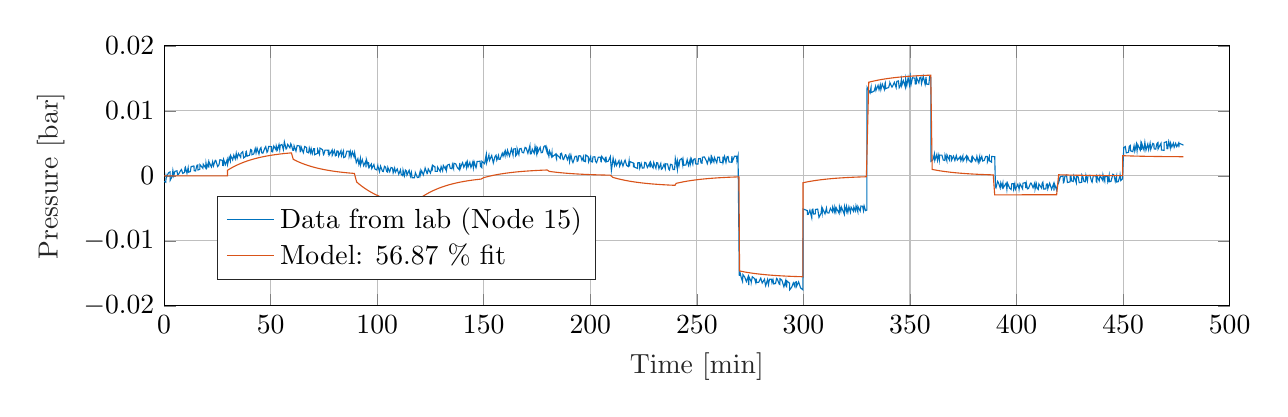
\begin{tikzpicture}

\begin{axis}[%
scaled y ticks = false,
 y tick label style={/pgf/number format/fixed,
/pgf/number format/1000 sep = \thinspace}, % Optional if you want to replace comma as the 1000 separator 
width=5.328in,
height=1.3in,
at={(1.011in,0.642in)},
scale only axis,
xmin=0,
xmax=500,
xlabel style={font=\color{white!15!black}},
xlabel={Time [min]},
ymin=-0.02,
ymax=0.02,
ylabel style={font=\color{white!15!black}},
ylabel={Pressure [bar]},
axis background/.style={fill=white},
%title style={font=\bfseries},
%title={Node 11},
xmajorgrids,
ymajorgrids,
legend style={at={(0.05,0.1)}, anchor=south west, legend cell align=left, align=left, draw=white!15!black}
]
\addplot [color=mycolor1]
  table[row sep=crcr]{%
0.000833333333333333	-0.000862377244981005\\
0.8175	-0.000988525827578635\\
0.978333333333333	-7.0686140385523e-05\\
1.10416666666667	-0.000263823970297061\\
2.0625	0.000467837808787119\\
2.795	0.000596596362057222\\
2.88	-0.000685769229336164\\
3.77583333333333	-0.000120275583229856\\
4.13333333333333	0.000830623732555297\\
4.56	2.06628331949343e-05\\
5.0675	0.000684465374763188\\
6.07	0.000778424319051119\\
6.32916666666667	0.000165081210515144\\
6.73916666666667	0.000204230770637248\\
7.6675	0.000749714641656574\\
8.16916666666667	0.000967212197835188\\
8.76916666666667	0.000370398903598079\\
9.66833333333333	0.000546136929025637\\
9.76666666666667	0.00120384953897001\\
9.98916666666667	0.00134043800428257\\
10.745	0.000386058727695787\\
11.3041666666667	0.0012447390795583\\
11.5191666666667	0.000565276713973328\\
12.3391666666667	0.000642705843958147\\
12.6816666666667	0.00142047710495177\\
14.0125	0.00151617602966467\\
14.1291666666667	0.000798434094232608\\
14.7733333333333	0.000741014739437829\\
15.4291666666667	0.00162231483709235\\
15.815	0.00167190427993347\\
15.9108333333333	0.000900222950550922\\
16.7816666666667	0.00100114181664962\\
16.865	0.00170844386936125\\
18.2058333333333	0.00115687006687296\\
18.385	0.00179370291142761\\
19.4766666666667	0.00122907925565102\\
19.6608333333333	0.00198945071194573\\
20.0525	0.00125517896234129\\
20.8758333333333	0.00211733927501684\\
20.9908333333333	0.00127779870815317\\
21.0633333333333	0.0021634487568204\\
22.2233333333333	0.00135435784778479\\
22.7958333333333	0.00217388863954085\\
23.175	0.00152748590254786\\
24.0383333333333	0.0023948661566206\\
24.2691666666667	0.00236963644025792\\
25.1275	0.00142395706589837\\
25.745	0.00167016429953976\\
26.2225	0.00247925520851283\\
27.4008333333333	0.00237224641086556\\
27.4858333333333	0.00160404504244099\\
27.8925	0.00158751522813219\\
27.9858333333333	0.00247142529645686\\
28.83	0.00171627378137743\\
29.6308333333333	0.00252797466143562\\
29.815	0.00179109294070628\\
30.5641666666667	0.00285422099560406\\
31.0891666666667	0.00229307730064335\\
31.2183333333333	0.00310303819978486\\
32.2	0.00244532559000532\\
32.7233333333333	0.00318742725159751\\
33.395	0.0025949639085607\\
33.8591666666667	0.00346582412358573\\
34.2908333333333	0.00271937251059995\\
34.9191666666667	0.00342580457323408\\
35.9508333333333	0.00283682119125758\\
36.0916666666667	0.00344233438742919\\
36.9125	0.00371638130825119\\
37.36	0.00275504211006961\\
38.2	0.00296731972474304\\
38.4108333333333	0.00371812128870175\\
38.5966666666667	0.00376771073160539\\
38.9675	0.00302038912844552\\
40.1083333333333	0.0031648075057629\\
40.6441666666667	0.00404697759363132\\
41.1508333333333	0.0039156090697898\\
41.185	0.00323788668475486\\
42.0633333333333	0.00335446537476089\\
42.77	0.00418791601011578\\
43.1608333333333	0.00352150349799246\\
43.635	0.00425229528676396\\
44.5241666666667	0.00334402549211432\\
45.0141666666667	0.00411744680189627\\
45.47	0.00433581434836838\\
45.8133333333333	0.00354238326347883\\
46.3525	0.0034858338986706\\
47.3441666666667	0.00428970486649091\\
47.6991666666667	0.00448110271605315\\
48.2991666666667	0.00362068238364061\\
48.67	0.00380860027214255\\
49.0625	0.00451590232495078\\
50.4233333333333	0.00448110271596222\\
50.5433333333333	0.00372856117158704\\
50.9183333333333	0.00367897172862655\\
51.48	0.00458637153314753\\
52.5641666666667	0.00397476840515451\\
52.6508333333333	0.00460551131801282\\
53.2016666666667	0.00402087788691829\\
53.9175	0.00479951913826795\\
54.2791666666667	0.00403740770135216\\
54.5333333333333	0.00470904015494086\\
55.3191666666667	0.00482648883518919\\
55.9791666666667	0.00402087788698652\\
56.4358333333333	0.00523625423107574\\
57.2616666666667	0.00411483683143074\\
57.4983333333333	0.00418791601019536\\
58.0175	0.00482735882565891\\
59.0475	0.00431319460272703\\
59.4583333333333	0.00493958756481702\\
59.71	0.00478124934387239\\
60.4483333333333	0.00390429919687818\\
60.7408333333333	0.00390516918701819\\
61.0058333333333	0.00462378111311323\\
61.8883333333333	0.00380164035016975\\
62.4391666666667	0.00465771073175716\\
63.5575	0.00458376156260243\\
63.9091666666667	0.00371812128890639\\
64.11	0.00377989059473663\\
64.3266666666667	0.00444456312683003\\
65.3441666666667	0.00355369313609485\\
66.0133333333333	0.00451677231543188\\
66.9083333333333	0.00433320437808477\\
66.9725	0.00365722197301152\\
67.8191666666667	0.00353542334144918\\
68.145	0.00427926498390122\\
68.7616666666667	0.00354064328265311\\
69.045	0.00414267651863981\\
69.5766666666667	0.00341449470020877\\
70.21	0.00418095608857499\\
70.6016666666667	0.00416442627416388\\
70.6825	0.00324397661591688\\
72.0133333333333	0.00347191405499786\\
72.0891666666667	0.00403740770139763\\
72.9233333333333	0.00330226596134622\\
73.1633333333333	0.00426099518930101\\
74.3633333333333	0.00401478795541521\\
74.7966666666667	0.00323701669413737\\
75.0066666666667	0.00332401571664293\\
75.5033333333333	0.00395475863000144\\
76.9916666666667	0.00393387886454918\\
77.1133333333333	0.00322309685085118\\
77.3091666666667	0.00400782803379485\\
77.4691666666667	0.00319438717336568\\
78.8875	0.00399129821933827\\
78.9266666666667	0.00317176742754241\\
79.9125	0.00391212910911606\\
80.3783333333333	0.00307258854187153\\
80.795	0.00313435784779273\\
81.0891666666667	0.0038199101452247\\
81.6866666666667	0.00380077036018889\\
81.8841666666667	0.00303517896200817\\
83.025	0.00387993947050205\\
83.2458333333333	0.00305692871789603\\
84.1691666666667	0.00382861004719331\\
84.2625	0.00280376156245807\\
85.04	0.00293426009603451\\
85.7833333333333	0.00380686029182839\\
86.7758333333333	0.00379816038926861\\
86.8625	0.0030299590208952\\
87.3991666666667	0.00373465110299917\\
87.7625	0.00292034025254367\\
88.3616666666667	0.00369550154301493\\
89.1225	0.00293165012547802\\
89.4233333333333	0.00357196293071779\\
90.1958333333333	0.00203991014501212\\
90.9566666666667	0.0026358534492229\\
91.405	0.00177195315573869\\
92.1141666666667	0.00268283292126312\\
92.1958333333333	0.00166929430943952\\
92.9875	0.0024966550132231\\
93.6625	0.0015579355602395\\
94.6725	0.00227741747642909\\
94.7633333333333	0.00131607827800878\\
94.9291666666667	0.00253232461214709\\
95.835	0.00153270584379156\\
95.94	0.00209819948987303\\
96.2541666666667	0.00128388863966761\\
97.2441666666667	0.00181023272567388\\
97.4675	0.0011159805262278\\
98.4533333333333	0.00172845364482696\\
98.9266666666667	0.00103594142529714\\
99.775	0.000896742989865806\\
100.281666666667	0.00155793556064879\\
100.296666666667	0.00151878600057359\\
101.095833333333	0.000640095873458507\\
101.571666666667	0.00149529626420103\\
102.484166666667	0.000700995189103243\\
102.878333333333	0.000657495677759523\\
103.423333333333	0.00145962666523161\\
103.9225	0.0013395680139493\\
104.438333333333	0.000665325589906451\\
104.8775	0.000568756675064896\\
104.994166666667	0.00129345853207183\\
105.878333333333	0.00062704601983482\\
106.505833333333	0.00129084856124251\\
107.181666666667	0.00118905970503788\\
107.499166666667	0.000462617867796389\\
108.180833333333	0.00119601962693111\\
108.555833333333	0.000556576811626713\\
109.411666666667	0.0010576911812987\\
110.121666666667	0.000249470262391749\\
110.926666666667	0.000931542598558793\\
111.284166666667	0.00021467065331221\\
111.963333333333	2.50127844392822e-05\\
112.130833333333	0.000877603204625349\\
112.793333333333	8.48296995997755e-06\\
113.264166666667	0.000889783067790695\\
113.729166666667	0.000744494700219589\\
113.975	9.4612002393718e-05\\
115.001666666667	0.00084628355699265\\
115.570833333333	-6.89461598002983e-05\\
116.055833333333	0.00054352695825316\\
116.37	-0.000296013608650308\\
117.455	-0.000306453490921677\\
117.931666666667	0.000453047975051107\\
117.933333333333	0.000465227838239157\\
118.875	-0.000268173921031983\\
119.449166666667	-0.000235114292482602\\
120.135833333333	0.000676635462977221\\
120.228333333333	8.5912100265928e-05\\
120.856666666667	0.000759284534350674\\
121.661666666667	0.000145941425406859\\
122.309166666667	0.000910662833083775\\
122.5025	0.00119862959741937\\
123.425	0.000321679451061818\\
123.5325	0.000349519138316323\\
123.965	0.00105247123966279\\
125	0.000426078278232184\\
125.630833333333	0.00126126889400352\\
125.713333333333	0.000717525003127828\\
126.1125	0.00160665501267346\\
127.129166666667	0.00136566772076463\\
127.2025	0.000691425296835468\\
128.213333333333	0.000687945335684226\\
128.324166666667	0.00134826791591791\\
129.563333333333	0.000672285511572279\\
129.9975	0.00142308707528088\\
130.71	0.0007671144459519\\
131.05	0.00158142529668026\\
132.150833333333	0.000967212198164868\\
132.25	0.00154923565733867\\
132.494166666667	0.000877603204761768\\
132.96	0.00165189450468375\\
133.8325	0.00176760320442468\\
134.286666666667	0.00114991014448521\\
135.051666666667	0.00108292089804224\\
135.301666666667	0.00173976351753397\\
135.864166666667	0.00112294044798461\\
135.98	0.00192768140628602\\
136.874166666667	0.00183198248147079\\
137.691666666667	0.00120645950915702\\
138.360833333333	0.00100723174765249\\
138.800833333333	0.00198684074099134\\
138.891666666667	0.00104725129868627\\
139.855	0.00190593165035266\\
140.0825	0.0020407801351294\\
140.648333333333	0.00131694826801237\\
141.668333333333	0.00206252989074443\\
141.895	0.00133086811198069\\
142.325	0.00209036957831726\\
142.671666666667	0.00139002744732267\\
143.463333333333	0.00206948981286501\\
143.9925	0.00129258854190908\\
144.855	0.00212429919702942\\
145.1375	0.00124038912864222\\
145.525833333333	0.00211298932395862\\
146.3775	0.00125082901105003\\
146.588333333333	0.00148398639163047\\
146.845833333333	0.00218954846364711\\
148.249166666667	0.00224957778919729\\
148.493333333333	0.00144048687985474\\
149.046666666667	0.00126213888407534\\
149.100833333333	0.0022530577500757\\
150.381666666667	0.00185808218758127\\
150.93	0.00290555041875365\\
151.185833333333	0.00330487593169806\\
151.315833333333	0.00198423077023022\\
152.4225	0.0032196168897454\\
152.716666666667	0.00238181630334935\\
153.73	0.00313087788650507\\
154.28	0.00231134709525491\\
154.488333333333	0.00198249079031398\\
155.300833333333	0.00298819948935403\\
155.774166666667	0.00317959733916637\\
156.128333333333	0.00241574592228885\\
156.925	0.00314044777902298\\
157.143333333333	0.00252449469995469\\
157.65	0.00252188472955736\\
158.68	0.00347191405536165\\
159.055833333333	0.00303169900135714\\
159.610833333333	0.0035867527640758\\
159.999166666667	0.00310303819965982\\
160.170833333333	0.00383382998807888\\
160.915	0.00315784758373325\\
161.173333333333	0.00392169900120196\\
162.105	0.00302821904070613\\
162.986666666667	0.00414789645993466\\
163.7325	0.00316045755458533\\
163.926666666667	0.00411918678188072\\
164.819166666667	0.0041679062349968\\
164.999166666667	0.00308476840496866\\
165.615833333333	0.00336403526699455\\
165.684166666667	0.00415920633232333\\
166.489166666667	0.00327877622504189\\
166.840833333333	0.00414702646986284\\
167.545	0.00421314572650686\\
168.046666666667	0.00359719264757502\\
168.7075	0.00353455335103633\\
169.391666666667	0.00437322392773154\\
169.875	0.00429492480744473\\
170.705	0.00346060418169969\\
171.666666666667	0.00465423077103794\\
171.854166666667	0.00336142529641534\\
172.333333333333	0.00340753477849745\\
172.7675	0.00410787690940112\\
173.685	0.00346495413296821\\
174.071666666667	0.00453591209980828\\
174.815833333333	0.00339187495429458\\
174.979166666667	0.00443151327277433\\
175.273333333333	0.00430710467090564\\
175.368333333333	0.00360154259820689\\
176.4625	0.00438018385003403\\
176.940833333333	0.00354847319423157\\
177.514166666667	0.00358936273515525\\
178.225	0.00451764230498072\\
178.795	0.00462639108314675\\
179.628333333333	0.00368506166001595\\
179.670833333333	0.00422358560927846\\
180.565833333333	0.00300646928472731\\
180.8875	0.00381295022299041\\
181.779166666667	0.00300733927493554\\
182.028333333333	0.00359806263682827\\
182.18	0.00290903037922277\\
183.8825	0.00338665501231758\\
183.956666666667	0.0027776618553699\\
184.155	0.0025775641037481\\
184.251666666667	0.00326746635219849\\
185.946666666667	0.00268283292099028\\
186.013333333333	0.00338752500302605\\
186.499166666667	0.00348061395689825\\
187.235	0.00250883487634296\\
187.446666666667	0.00249230506165901\\
188.320833333333	0.0032474565772273\\
188.546666666667	0.00322222686064294\\
189.2525	0.00246359538433266\\
190.034166666667	0.00317176742720135\\
190.2825	0.00218258854129913\\
190.9025	0.00320308707537975\\
191.515	0.00227654748610717\\
191.854166666667	0.00202599030154402\\
192.8425	0.00298123956827936\\
193.593333333333	0.00302560906953572\\
193.8425	0.0022373979264185\\
194.166666666667	0.00230090721234688\\
194.634166666667	0.00308911835587339\\
195.445	0.00306562862038759\\
196.076666666667	0.00237920633254277\\
196.824166666667	0.00298993946986145\\
196.936666666667	0.00226610760356294\\
197.719166666667	0.00217910858164855\\
197.880833333333	0.00320569704609538\\
199.003333333333	0.00294991992055571\\
199.185833333333	0.0021425689921753\\
200.135833333333	0.00293687006665919\\
200.343333333333	0.00221216820947034\\
200.9975	0.00212864914793415\\
201.225833333333	0.00289337055529273\\
202.134166666667	0.00293339010537153\\
202.4375	0.00222608805343866\\
202.948333333333	0.00202425032094566\\
203.750833333333	0.00285248101500571\\
204.869166666667	0.00287597075053697\\
204.950833333333	0.00220259831749814\\
205.1075	0.00216518873736191\\
205.373333333333	0.00300385931387523\\
206.978333333333	0.00220172832678969\\
207.045833333333	0.00282986126868223\\
207.3425	0.00286988081917031\\
207.628333333333	0.00216431874683537\\
208.409166666667	0.00224435784785698\\
209.395	0.00294904992966535\\
209.41	0.00283508120988615\\
209.890833333333	0.000817573879120626\\
210.710833333333	0.00271676253997527\\
211.365	0.00162057485627798\\
211.861666666667	0.00231221708532672\\
212.278333333333	0.00159012519885351\\
213.463333333333	0.00233048687951765\\
213.763333333333	0.00147267651851421\\
213.923333333333	0.00160404504213971\\
214.576666666667	0.00227132754526707\\
215.310833333333	0.00150486615662798\\
216.0225	0.00221390818988682\\
216.328333333333	0.00240878600003186\\
217.040833333333	0.00159186517922449\\
217.804166666667	0.00142221708530002\\
218.205	0.00232787690943864\\
218.429166666667	0.00143874689989304\\
218.511666666667	0.00219563839555945\\
220.188333333333	0.00197553086837529\\
220.293333333333	0.00131346830749776\\
220.455833333333	0.00200076058518703\\
220.660833333333	0.00134913790626257\\
222.145	0.00113338033061977\\
222.251666666667	0.00199902060445226\\
222.985	0.00202425032130946\\
223.200833333333	0.00119079968509056\\
223.870833333333	0.00190245168920142\\
224.4375	0.00118035980268275\\
225.213333333333	0.00122559929455662\\
225.553333333333	0.00207557974436809\\
226.069166666667	0.00201642040848043\\
226.773333333333	0.00127605872804365\\
227.98	0.00204513008694363\\
228.039166666667	0.00127692871802451\\
228.39	0.00198945071298026\\
229.1325	0.00133521806202139\\
229.473333333333	0.0012029795495519\\
229.759166666667	0.00205035002892059\\
230.793333333333	0.00116209000799158\\
231.1575	0.00201903038160622\\
231.645	0.00198336078138622\\
232.1875	0.00110467065388462\\
233.070833333333	0.00189027182705928\\
233.34	0.000998531844842609\\
233.754166666667	0.00110989059467925\\
234.61	0.001784133018472\\
235.170833333333	0.00112207045677593\\
235.339166666667	0.0018485122964276\\
236.2375	0.00182676253999403\\
236.8175	0.00102376156229098\\
237.163333333333	0.000889783066767513\\
237.6175	0.00177108316439359\\
238.295	0.00173019362601651\\
238.8225	0.000968952178490384\\
239.544166666667	0.000966342207456422\\
239.885833333333	0.00267326302883616\\
240.835833333333	0.00104551131872455\\
240.925	0.00230525716470681\\
241.571666666667	0.00146832656874635\\
242.019166666667	0.00245576547314072\\
242.938333333333	0.00267152304887447\\
243.39	0.00169104406541834\\
243.5775	0.00236528648984774\\
243.885	0.00162318482763027\\
244.8525	0.00166233438777369\\
245.450833333333	0.0024949150324656\\
246.0675	0.00161013497491608\\
246.874166666667	0.00251318482779339\\
246.966666666667	0.00184677231664779\\
247.445833333333	0.00255842432025843\\
248.108333333333	0.00179109294122923\\
248.373333333333	0.00250883487625203\\
249.150833333333	0.00262976351796992\\
249.403333333333	0.00183894240345495\\
250.485	0.00178674298959691\\
250.793333333333	0.00262367358573926\\
251.594166666667	0.00266369313650017\\
251.97	0.0019746608783035\\
252.403333333333	0.00194160125102741\\
252.651666666667	0.00287249079047711\\
253.555	0.00290207045664745\\
254.535	0.00222956801472635\\
254.8875	0.00187635198236336\\
255.633333333333	0.00277766185464232\\
256.435833333333	0.00202686029134297\\
256.62	0.00266456312584437\\
256.940833333333	0.00194682119109443\\
257.060833333333	0.00285683096563757\\
257.984166666667	0.00211298932391316\\
258.2475	0.00282290134674354\\
259.336666666667	0.00201120046732201\\
259.778333333333	0.00286379088830388\\
260.62	0.00285596097611149\\
260.818333333333	0.00210167945143352\\
262.106666666667	0.0020225103407111\\
262.2775	0.0029438299887343\\
262.363333333333	0.00214604895246254\\
263.005	0.00299080946006966\\
263.665	0.00205904993018435\\
264.185833333333	0.00292817016416763\\
264.6325	0.00297601962675714\\
265.093333333333	0.00213212910913085\\
266.3125	0.00208862959780987\\
266.419166666667	0.00302647905947112\\
266.7525	0.00228872734961355\\
267.645833333333	0.00300472930476559\\
268.635	0.00300907925512461\\
268.81	0.00231134709584607\\
269.328333333333	0.00307693849318555\\
269.913333333333	-0.015393823970854\\
270.196666666667	-0.014779610872657\\
270.82	-0.0156774407831026\\
271.43	-0.016256854271879\\
271.600833333333	-0.0151998161508263\\
272.438333333333	-0.0155547721616958\\
273.225	-0.0162638141946363\\
274.0575	-0.0155191025626581\\
274.330833333333	-0.0168101680560457\\
274.444166666667	-0.0155260624844149\\
275.539166666667	-0.0163203635590352\\
275.544166666667	-0.0163455932756651\\
275.996666666667	-0.0155321524152814\\
277.0725	-0.0158079393173384\\
277.6475	-0.0164386822305377\\
277.903333333333	-0.0158279490915365\\
278.004166666667	-0.0164117125318543\\
278.998333333333	-0.0163925727480918\\
279.9175	-0.0157809696198373\\
279.980833333333	-0.0157435600413837\\
280.660833333333	-0.0164987115552239\\
281.735833333333	-0.0158992882908851\\
282.070833333333	-0.0166257301272626\\
282.285	-0.01691021693122\\
283.173333333333	-0.0159593176152075\\
283.5875	-0.0167518787103208\\
284.071666666667	-0.0159027682511723\\
284.980833333333	-0.0159132081336711\\
285.256666666667	-0.0164613019745875\\
285.7075	-0.0159610575966244\\
286.09	-0.0166335600390912\\
286.9125	-0.0165709207442805\\
287.386666666667	-0.0157853195707421\\
287.720833333333	-0.0158731885841834\\
288.6525	-0.0166500898541844\\
288.929166666667	-0.0167153391213933\\
289.023333333333	-0.0158253391212301\\
289.878333333333	-0.0160454466485052\\
290.838333333333	-0.0170737750937323\\
291.6575	-0.0161333156609462\\
291.740833333333	-0.0168849872144992\\
292.123333333333	-0.0170476753872126\\
292.233333333333	-0.0161707252399455\\
293.479166666667	-0.0165126313979189\\
293.5675	-0.0175261700112887\\
294.5175	-0.017128584479261\\
295.258333333333	-0.0164604319846066\\
295.928333333333	-0.0170015659056762\\
296.0275	-0.0164021426410645\\
296.6475	-0.0163142736278959\\
296.7375	-0.0170120057876292\\
297.72	-0.0163203635599447\\
298.658333333333	-0.0172434231874749\\
299.755	-0.0175435698158171\\
299.785833333333	-0.014556893374166\\
299.785833333333	-0.014556893374166\\
299.8575	-0.00510270960002429\\
301.7975	-0.00534804684447493\\
301.893333333333	-0.0059422501668368\\
302.256666666667	-0.00592137040229404\\
303.024166666667	-0.0053010673716844\\
303.899166666667	-0.00646598428265038\\
304.065	-0.00519579855362368\\
304.433333333333	-0.00513054928741524\\
304.768333333333	-0.0058848308119113\\
305.5725	-0.0058500312035821\\
305.656666666667	-0.00517839874909526\\
306.694166666667	-0.00511488946339428\\
307.300833333333	-0.00638768516218163\\
308.258333333333	-0.00576999210260595\\
308.556666666667	-0.00502702045149903\\
308.829166666667	-0.00563079366656069\\
308.9325	-0.00500092074388789\\
310.124166666667	-0.00586221106613352\\
310.801666666667	-0.00496873110550128\\
310.81	-0.00495742123274881\\
311.128333333333	-0.00568995300172076\\
311.961666666667	-0.00572040265923618\\
312.656666666667	-0.00500353071437615\\
313.6775	-0.0055664143889689\\
313.773333333333	-0.00479212309027474\\
314.640833333333	-0.00558642416562266\\
314.740833333333	-0.00486346228907764\\
315.233333333333	-0.00548550529873951\\
315.401666666667	-0.00492610158434303\\
316.764166666667	-0.00578391194575573\\
316.910833333333	-0.00471730393136655\\
317.558333333333	-0.00545679562264098\\
317.795	-0.00479734303206983\\
319.186666666667	-0.00590919053746888\\
319.295833333333	-0.00465292465522993\\
320.079166666667	-0.00548115534728907\\
320.259166666667	-0.00474949356902557\\
320.855833333333	-0.00563253364725\\
321.34	-0.00475819347156262\\
322.064166666667	-0.00560991390074464\\
322.395	-0.00483388262026979\\
323.494166666667	-0.00546810549412016\\
323.649166666667	-0.0048016929823379\\
324.426666666667	-0.00539589630579115\\
324.685	-0.00460594518234841\\
325.520833333333	-0.00552900480887814\\
325.598333333333	-0.00474427362914043\\
326.635833333333	-0.0054289559346134\\
326.971666666667	-0.00465031468310456\\
327.758333333333	-0.00467902436147682\\
328.1825	-0.0053680566184002\\
328.481666666667	-0.00463030490854266\\
329.129166666667	-0.00535239679474303\\
329.7375	-0.00528018760504978\\
329.855	0.0136394898131667\\
331.24	0.0127468798428791\\
331.746666666667	0.0136212200186574\\
331.748333333333	0.0136116501261395\\
331.786666666667	0.0128121291094513\\
333.1475	0.0130261467051324\\
333.826666666667	0.013738668698451\\
334.043333333333	0.0131392454329299\\
335.023333333333	0.013920496654745\\
335.4775	0.0132662640064237\\
336.064166666667	0.0140005357558121\\
336.336666666667	0.0132714839483097\\
336.995833333333	0.0141179844348781\\
338.023333333333	0.0132749639091426\\
338.2725	0.0141919336058064\\
338.403333333333	0.0143154722161026\\
338.635	0.013419382285164\\
339.981666666667	0.0135829404481311\\
340.563333333333	0.014251092939966\\
340.579166666667	0.0143302620504156\\
341.543333333333	0.0136386198225492\\
341.6875	0.0136890792546265\\
342.685833333333	0.01438855139514\\
343.508333333333	0.0135716305748329\\
343.829166666667	0.0145329697725256\\
344.575	0.0146043089718742\\
344.946666666667	0.0135385709460107\\
345.494166666667	0.0138735171829549\\
345.9675	0.0147913568695995\\
346.133333333333	0.0138700372222129\\
346.874166666667	0.0146556383950238\\
347.8575	0.0136177400567331\\
347.946666666667	0.014883575835037\\
348.5125	0.0139091867828111\\
349.1075	0.0151089033019244\\
349.761666666667	0.0139544262727296\\
350.17	0.0151611027156915\\
350.508333333333	0.014051865178416\\
351.175833333333	0.0150862835561466\\
352.27	0.0150297341925662\\
352.4925	0.0141223343883294\\
352.9525	0.0141536540351891\\
353.026666666667	0.0151497928425752\\
354.1625	0.0143032923530964\\
354.589166666667	0.0150801936246435\\
355.118333333333	0.0151819824813256\\
355.4125	0.0141928035950596\\
356.226666666667	0.0153055210938046\\
357.095	0.0140823148371138\\
357.539166666667	0.0152220020310861\\
357.7575	0.0141188544261323\\
358.846666666667	0.0140527351692154\\
359.215	0.0152533216797647\\
359.765833333333	0.0151358729988797\\
359.859166666667	0.00224609782754584\\
360.8	0.00247838521773616\\
361.456666666667	0.00335620535452932\\
361.638333333333	0.00235658658667404\\
362.573333333333	0.00328225618596575\\
362.908333333333	0.0023765963624183\\
363.494166666667	0.00321526693797666\\
363.781666666667	0.00248969509121622\\
363.945833333333	0.00317002744587541\\
364.9825	0.00318742725049476\\
365.603333333333	0.00243227573674545\\
366.3225	0.00236615648019239\\
366.445833333333	0.00319960711413755\\
367.288333333333	0.00231830701705718\\
367.373333333333	0.00320134709373548\\
368.564166666667	0.00239399616594624\\
368.625	0.0031265279356458\\
369.388333333333	0.00304648883521538\\
369.536666666667	0.00241835589277711\\
370.421666666667	0.00303865892302299\\
371.066666666667	0.00235658658731069\\
371.721666666667	0.0031160880519647\\
372.2275	0.00241835589304998\\
373.543333333333	0.00295165990029006\\
373.626666666667	0.0024253158150796\\
373.7325	0.00306475862945177\\
373.9025	0.00235310662647775\\
374.815833333333	0.00309259831584227\\
374.9	0.00226871757414215\\
376.505833333333	0.00307084856186435\\
376.654166666667	0.00237311640122156\\
377.134166666667	0.00289163057514913\\
377.76	0.00237137642007751\\
378.6625	0.00210515941226647\\
379.100833333333	0.00303082901037585\\
379.1725	0.00212516918819261\\
379.254166666667	0.00300124934329601\\
380.881666666667	0.00224696781925474\\
381.325	0.00284813106464668\\
381.396666666667	0.00297949958795385\\
382.034166666667	0.00206774983263044\\
382.696666666667	0.00296035980182666\\
382.793333333333	0.00223565794632036\\
383.686666666667	0.00299863937208017\\
384.123333333333	0.00227132754463041\\
384.8175	0.00236354651024981\\
385.525833333333	0.00298210955798736\\
386.260833333333	0.00298732949941866\\
386.345	0.00216170877693828\\
387.2125	0.00297340965599602\\
387.3025	0.00230177720250963\\
388.243333333333	0.00210776938284568\\
388.3425	0.00297166967530671\\
389.763333333333	0.00295339988152507\\
390.100833333333	-0.00172627753881074\\
390.3475	-0.00185329611121318\\
391.105833333333	-0.000844977440548011\\
391.411666666667	-0.000990265808096358\\
392.323333333333	-0.00185851605337206\\
392.613333333333	-0.00107465485915867\\
393.215833333333	-0.00170104782008906\\
393.5975	-0.00109205466386897\\
393.7675	-0.00185590608070102\\
395.1125	-0.00112424430252844\\
395.47	-0.00208297352946005\\
395.775833333333	-0.00113555417464425\\
396.765	-0.00190462553290757\\
397.470833333333	-0.00210385329573087\\
397.795833333333	-0.00119906346034526\\
398.595833333333	-0.00119384352018728\\
398.675833333333	-0.00198031468216045\\
399.1925	-0.00122516316913873\\
399.4725	-0.00209428340184872\\
400.604166666667	-0.00130085231775495\\
401.171666666667	-0.00198466463515701\\
401.196666666667	-0.00205078389134628\\
401.628333333333	-0.00123038310920578\\
402.835	-0.00199075456584155\\
403.006666666667	-0.00114512406752595\\
404.165833333333	-0.00103811527059491\\
404.3375	-0.00189940559284055\\
404.594166666667	-0.00117383374489777\\
405.113333333333	-0.0020107643408582\\
405.621666666667	-0.00194290510370679\\
406.5775	-0.00111728438031691\\
406.9	-0.00113642416453416\\
407.753333333333	-0.00183241634530618\\
408.5525	-0.00109118467316052\\
408.6975	-0.00204208398808164\\
409.289166666667	-0.00125039288476814\\
409.549166666667	-0.00185503609026541\\
410.180833333333	-0.00210385329445756\\
410.48	-0.00125648281618027\\
411.750833333333	-0.00189940559274959\\
411.983333333333	-0.00117644371638648\\
412.351666666667	-0.000979825924688094\\
412.745	-0.00204817392031231\\
413.764166666667	-0.00201424430187302\\
414.011666666667	-0.00127127265094801\\
414.4525	-0.00126170275742965\\
414.673333333333	-0.00199510451711007\\
415.541666666667	-0.00112859425352413\\
416.43	-0.0020551338417053\\
417.440833333333	-0.00117296375491691\\
417.5375	-0.00226828144804217\\
417.8075	-0.00126431272846361\\
418.785833333333	-0.00216997255292056\\
418.8325	-0.0019994544689243\\
419.835833333333	-0.000588330325163894\\
419.920833333333	-0.000864117225674754\\
420.6075	-0.000131585456793759\\
421.823333333333	-2.71866295324386e-05\\
421.98	-0.00106247499624346\\
422.223333333333	-0.000996355739872279\\
422.679166666667	-6.98161511454021e-05\\
423.459166666667	0.000105921874009318\\
423.869166666667	-0.00103637528990561\\
425.095833333333	-0.000938066394965908\\
425.179166666667	-5.32863377802062e-05\\
425.536666666667	-3.69689413759478e-06\\
425.801666666667	-0.000776248211869585\\
426.589166666667	-0.000880647038949023\\
426.874166666667	-8.91683575077185e-06\\
428.054166666667	-0.00108422475240416\\
428.138333333333	9.35295903131683e-06\\
428.898333333333	-0.000168995037612085\\
429.430833333333	-0.00105812504633918\\
430.57	-0.000995485751346614\\
430.653333333333	0.00015551131683339\\
431.075833333333	-8.98259267987089e-05\\
431.633333333333	-0.0008823870210935\\
432.284166666667	-0.000924146550815685\\
432.5625	7.46022260582901e-05\\
433.259166666667	-0.000796257988796178\\
433.4975	8.4829688685728e-06\\
434.400833333333	8.76520802276515e-05\\
435.24	-0.000877167079298441\\
435.448333333333	-0.000988525827498005\\
436.005833333333	-2.54466498435524e-05\\
437.294166666667	3.2842694971863e-05\\
437.3325	-0.000845847430983621\\
437.66	-0.000966776071428227\\
437.73	-4.98063753102129e-05\\
438.799166666667	-0.000762328369083604\\
439.176666666667	4.41525681790789e-05\\
440.490833333333	-0.00074405857521101\\
440.573333333333	0.000148551395167534\\
441.400833333333	-0.000818877734301116\\
441.530833333333	-3.84965035581941e-05\\
442.544166666667	-9.15659068513874e-05\\
442.800833333333	-0.000857157304554629\\
443.430833333333	5.0242498772668e-05\\
443.515	-0.000911966687445726\\
444.310833333333	-0.000862377243894069\\
445.189166666667	0.000239030377732929\\
445.754166666667	0.000105921873827408\\
446.314166666667	-0.000843237460222496\\
446.9075	-6.80761712746336e-05\\
446.956666666667	-0.000960686141016548\\
447.704166666667	-0.000907616736268158\\
448.571666666667	5.45924499502359e-05\\
448.588333333333	0.000103311901974906\\
448.915833333333	-0.000734488682965939\\
449.685	-0.000463051732177477\\
450.311666666667	0.00435930408358132\\
451.04	0.00449937251151739\\
451.493333333333	0.00352846341985155\\
452.55	0.00363025227562416\\
452.861666666667	0.00453417212048321\\
453.338333333333	0.00468555041944371\\
453.504166666667	0.00384165990099888\\
454.538333333333	0.00371812128906554\\
455.141666666667	0.00461943116198113\\
455.49	0.00380599030187029\\
456.235	0.00488825814337276\\
456.558333333333	0.00384774983268385\\
456.884166666667	0.0047768993926266\\
458.051666666667	0.00395649861012232\\
458.320833333333	0.00491087788824104\\
458.7675	0.00401565794564618\\
458.814166666667	0.00492392774068237\\
459.786666666667	0.00395475863079725\\
460.214166666667	0.00513881532643523\\
460.74	0.00395475862934205\\
461.5775	0.0048752082861111\\
461.980833333333	0.00402435784800134\\
462.670833333333	0.00501353673390356\\
462.975	0.00405654748811599\\
463.935833333333	0.00499178697974373\\
464.454166666667	0.0048926080928223\\
464.538333333333	0.00414093653599509\\
465.310833333333	0.00410178697639738\\
465.829166666667	0.00492827769158707\\
466.35	0.00512663546124628\\
466.398333333333	0.00411309684969552\\
467.783333333333	0.00501179675394184\\
468.009166666667	0.00396606850300402\\
469.206666666667	0.00391821904177875\\
469.273333333333	0.00510575569624877\\
470.3725	0.00525626400468268\\
470.588333333333	0.00418878599922123\\
470.9375	0.00417051620753142\\
471.418333333333	0.00526496390740164\\
472.1225	0.00429405481828241\\
472.314166666667	0.005022236635713\\
472.850833333333	0.00444456312598873\\
473.5675	0.00502136664527739\\
473.9475	0.00437844386979946\\
474.659166666667	0.00499178697465055\\
475.185833333333	0.00448284269787932\\
476.081666666667	0.00504485638158172\\
476.175833333333	0.00439323370338485\\
476.281666666667	0.00501788668317119\\
478.334166666667	0.00472035002659055\\
};
\addlegendentry{Data from lab (Node 15)}

\addplot [color=mycolor2]
  table[row sep=crcr]{%
0.000833333333333333	-1.06299307848883e-14\\
0.000833333333333333	-1.06299307848883e-14\\
1.10333333333333	-1.10236841397228e-14\\
1.10333333333333	-1.10236841397228e-14\\
2.20583333333333	-1.13893336919826e-14\\
2.20583333333333	-1.13893336919826e-14\\
3.3075	-1.17286380516017e-14\\
3.3075	-1.17286380516017e-14\\
4.41	-1.20439721327157e-14\\
4.41	-1.20439721327157e-14\\
5.51166666666667	-1.23365862704803e-14\\
5.51166666666667	-1.23365862704803e-14\\
6.61416666666667	-1.26085285772534e-14\\
6.61416666666667	-1.26085285772534e-14\\
7.71666666666667	-1.28610612388579e-14\\
7.71666666666667	-1.28610612388579e-14\\
8.81833333333333	-1.30953988238462e-14\\
8.81833333333333	-1.30953988238462e-14\\
9.92083333333333	-1.33131815458712e-14\\
9.92083333333333	-1.33131815458712e-14\\
11.0225	-1.351527293796e-14\\
11.0225	-1.351527293796e-14\\
12.125	-1.37030875109793e-14\\
12.125	-1.37030875109793e-14\\
13.2266666666667	-1.38773699708691e-14\\
13.2266666666667	-1.38773699708691e-14\\
14.3291666666667	-1.40393401837049e-14\\
14.3291666666667	-1.40393401837049e-14\\
15.4316666666667	-1.41897499137445e-14\\
15.4316666666667	-1.41897499137445e-14\\
16.5333333333333	-1.43293225641585e-14\\
16.5333333333333	-1.43293225641585e-14\\
17.6358333333333	-1.44590350544912e-14\\
17.6358333333333	-1.44590350544912e-14\\
18.7375	-1.45794017093795e-14\\
18.7375	-1.45794017093795e-14\\
19.84	-1.46912650186472e-14\\
19.84	-1.46912650186472e-14\\
20.9425	-1.47951441816965e-14\\
20.9425	-1.47951441816965e-14\\
22.0441666666667	-1.48915388105929e-14\\
22.0441666666667	-1.48915388105929e-14\\
23.1466666666667	-1.49811236062656e-14\\
23.1466666666667	-1.49811236062656e-14\\
24.2483333333333	-1.50642537825218e-14\\
24.2483333333333	-1.50642537825218e-14\\
25.3508333333333	-1.51415111975814e-14\\
25.3508333333333	-1.51415111975814e-14\\
26.4525	-1.52132021857983e-14\\
26.4525	-1.52132021857983e-14\\
27.555	-1.52798285383713e-14\\
27.555	-1.52798285383713e-14\\
28.6575	-1.53416994930893e-14\\
29.7516666666667	-1.53987359478708e-14\\
29.7591666666667	0.000848848970183772\\
29.7591666666667	0.000848848970183772\\
30.8616666666667	0.0010697096966788\\
30.8616666666667	0.0010697096966788\\
31.9633333333333	0.00127465732181676\\
31.9633333333333	0.00127465732181676\\
33.0658333333333	0.00146512634827416\\
33.0658333333333	0.00146512634827416\\
34.1675	0.00164187200719812\\
34.1675	0.00164187200719812\\
35.27	0.00180613140548664\\
35.27	0.00180613140548664\\
36.3725	0.00195866693236207\\
36.3725	0.00195866693236207\\
37.4741666666667	0.00210021221512194\\
37.4741666666667	0.00210021221512194\\
38.5766666666667	0.00223175798047907\\
38.5766666666667	0.00223175798047907\\
39.6783333333333	0.00235382582221238\\
39.6783333333333	0.00235382582221238\\
40.7808333333333	0.00246727013736849\\
40.7808333333333	0.00246727013736849\\
41.8833333333333	0.00257261746338855\\
41.8833333333333	0.00257261746338855\\
42.985	0.00267037447354188\\
42.985	0.00267037447354188\\
44.0875	0.00276122540455779\\
44.0875	0.00276122540455779\\
45.1891666666667	0.00284553049061255\\
45.1891666666667	0.00284553049061255\\
46.2916666666667	0.00292387981354539\\
46.2916666666667	0.00292387981354539\\
47.3933333333333	0.00299658403724817\\
47.3933333333333	0.00299658403724817\\
48.4958333333333	0.00306415204492175\\
48.4958333333333	0.00306415204492175\\
49.5983333333333	0.00312689744492808\\
49.5983333333333	0.00312689744492808\\
50.7	0.00318512201442808\\
50.7	0.00318512201442808\\
51.8025	0.00323923328827717\\
51.8025	0.00323923328827717\\
52.9041666666667	0.00328944582377207\\
52.9041666666667	0.00328944582377207\\
54.0066666666667	0.00333611107663962\\
54.0066666666667	0.00333611107663962\\
55.1091666666667	0.00337944563774902\\
55.1091666666667	0.00337944563774902\\
56.2108333333333	0.00341965792685407\\
56.2108333333333	0.00341965792685407\\
57.3133333333333	0.00345702940433425\\
57.3133333333333	0.00345702940433425\\
58.415	0.00349170825230784\\
58.415	0.00349170825230784\\
59.5175	0.00352393720059522\\
59.7516666666667	0.003530480593665\\
60.6191666666667	0.00253132047794515\\
60.6191666666667	0.00253132047794515\\
61.7216666666667	0.0023506496846869\\
61.7216666666667	0.0023506496846869\\
62.8241666666667	0.00218287411185638\\
62.8241666666667	0.00218287411185638\\
63.9258333333333	0.00202718683438764\\
63.9258333333333	0.00202718683438764\\
65.0283333333333	0.00188249814062357\\
65.0283333333333	0.00188249814062357\\
66.13	0.00174823432359349\\
66.13	0.00174823432359349\\
67.2325	0.00162345562220113\\
67.2325	0.00162345562220113\\
68.3341666666667	0.00150766727483855\\
68.3341666666667	0.00150766727483855\\
69.4366666666667	0.00140005883691511\\
69.4366666666667	0.00140005883691511\\
70.5391666666667	0.00130013085747577\\
70.5391666666667	0.00130013085747577\\
71.6408333333333	0.00120740272787148\\
71.6408333333333	0.00120740272787148\\
72.7433333333333	0.00112122541032975\\
72.7433333333333	0.00112122541032975\\
73.845	0.00104125720207823\\
73.845	0.00104125720207823\\
74.9475	0.000966938376656612\\
74.9475	0.000966938376656612\\
76.05	0.000897923992636168\\
76.05	0.000897923992636168\\
77.1516666666667	0.000833882121861701\\
77.1516666666667	0.000833882121861701\\
78.2541666666667	0.000774364512078682\\
78.2541666666667	0.000774364512078682\\
79.3558333333333	0.000719135169259283\\
79.3558333333333	0.000719135169259283\\
80.4583333333333	0.000667807523224775\\
80.4583333333333	0.000667807523224775\\
81.56	0.000620178054076348\\
81.56	0.000620178054076348\\
82.6625	0.000575913385904306\\
82.6625	0.000575913385904306\\
83.765	0.000534808069849699\\
83.765	0.000534808069849699\\
84.8666666666667	0.000496664407825086\\
84.8666666666667	0.000496664407825086\\
85.9691666666667	0.000461215418521333\\
85.9691666666667	0.000461215418521333\\
87.0708333333333	0.000428320542702345\\
87.0708333333333	0.000428320542702345\\
88.1733333333333	0.000397749537215169\\
88.1733333333333	0.000397749537215169\\
89.2758333333333	0.000369360510604255\\
89.2758333333333	0.000369360510604255\\
90.3775	-0.000956621405166064\\
90.3775	-0.000956621405166064\\
91.48	-0.00126360549537707\\
91.48	-0.00126360549537707\\
92.5816666666667	-0.001548471262335\\
92.5816666666667	-0.001548471262335\\
93.6841666666667	-0.00181321258474337\\
93.6841666666667	-0.00181321258474337\\
94.7858333333333	-0.00205887919177003\\
94.7858333333333	-0.00205887919177003\\
95.8883333333333	-0.00228719059299726\\
95.8883333333333	-0.00228719059299726\\
96.9908333333333	-0.00249920646691819\\
96.9908333333333	-0.00249920646691819\\
98.0925	-0.00269594651455455\\
98.0925	-0.00269594651455455\\
99.195	-0.0028787877907743\\
99.195	-0.0028787877907743\\
100.296666666667	-0.00304845528183579\\
100.296666666667	-0.00304845528183579\\
101.399166666667	-0.00320613655197583\\
101.399166666667	-0.00320613655197583\\
102.500833333333	-0.0033524568251941\\
102.500833333333	-0.0033524568251941\\
103.603333333333	-0.00348844025009153\\
103.603333333333	-0.00348844025009153\\
104.705833333333	-0.00361471797653627\\
104.705833333333	-0.00361471797653627\\
105.8075	-0.00373189734361245\\
105.8075	-0.00373189734361245\\
106.91	-0.00384079853216176\\
106.91	-0.00384079853216176\\
108.011666666667	-0.00394185334766509\\
108.011666666667	-0.00394185334766509\\
109.114166666667	-0.00403576910938609\\
109.114166666667	-0.00403576910938609\\
110.216666666667	-0.0041229817154548\\
110.216666666667	-0.0041229817154548\\
111.318333333333	-0.00420391061929196\\
111.318333333333	-0.00420391061929196\\
112.420833333333	-0.0042791222716143\\
112.420833333333	-0.0042791222716143\\
113.5225	-0.00434891489509602\\
113.5225	-0.00434891489509602\\
114.625	-0.00441377699359322\\
114.625	-0.00441377699359322\\
115.726666666667	-0.0044739657526335\\
115.726666666667	-0.0044739657526335\\
116.829166666667	-0.00452990245514641\\
116.829166666667	-0.00452990245514641\\
117.931666666667	-0.00458184672426213\\
117.931666666667	-0.00458184672426213\\
119.033333333333	-0.00463004838855863\\
119.751666666667	-0.00465961059036997\\
120.135833333333	-0.003439975737444\\
120.135833333333	-0.003439975737444\\
121.2375	-0.00319462926775687\\
121.2375	-0.00319462926775687\\
122.34	-0.00296661538765183\\
122.34	-0.00296661538765183\\
123.4425	-0.00275487579954256\\
123.4425	-0.00275487579954256\\
124.544166666667	-0.00255839213121748\\
124.544166666667	-0.00255839213121748\\
125.646666666667	-0.00237578912230021\\
125.646666666667	-0.00237578912230021\\
126.748333333333	-0.00220634273128924\\
126.748333333333	-0.00220634273128924\\
127.850833333333	-0.00204886694150715\\
127.850833333333	-0.00204886694150715\\
128.9525	-0.00190273734370701\\
128.9525	-0.00190273734370701\\
130.055	-0.00176693112389424\\
130.055	-0.00176693112389424\\
131.1575	-0.00164081795467565\\
131.1575	-0.00164081795467565\\
132.259166666667	-0.0015237912884134\\
132.259166666667	-0.0015237912884134\\
133.361666666667	-0.00141503201307389\\
133.361666666667	-0.00141503201307389\\
134.463333333333	-0.00131410888587834\\
134.463333333333	-0.00131410888587834\\
135.565833333333	-0.00122031550929724\\
135.565833333333	-0.00122031550929724\\
136.6675	-0.00113327998202618\\
136.6675	-0.00113327998202618\\
137.77	-0.00105239311087868\\
137.77	-0.00105239311087868\\
138.8725	-0.000977279469672488\\
138.8725	-0.000977279469672488\\
139.974166666667	-0.00090757779556783\\
139.974166666667	-0.00090757779556783\\
141.076666666667	-0.00084280022129624\\
141.076666666667	-0.00084280022129624\\
142.178333333333	-0.000782689896478222\\
142.178333333333	-0.000782689896478222\\
143.280833333333	-0.000726826087173768\\
143.280833333333	-0.000726826087173768\\
144.383333333333	-0.000674949508577335\\
144.383333333333	-0.000674949508577335\\
145.485	-0.000626810657671846\\
145.485	-0.000626810657671846\\
146.5875	-0.000582072593200155\\
146.5875	-0.000582072593200155\\
147.689166666667	-0.000540557923696663\\
147.689166666667	-0.000540557923696663\\
148.791666666667	-0.000501976072949651\\
148.791666666667	-0.000501976072949651\\
149.893333333333	-0.000290308461601277\\
149.893333333333	-0.000290308461601277\\
150.995833333333	-0.000192479471143182\\
150.995833333333	-0.000192479471143182\\
152.098333333333	-0.000101632939628477\\
152.098333333333	-0.000101632939628477\\
153.2	-1.7331936089132e-05\\
153.2	-1.7331936089132e-05\\
154.3025	6.10135927390518e-05\\
154.3025	6.10135927390518e-05\\
155.404166666667	0.000133714295703912\\
155.404166666667	0.000133714295703912\\
156.506666666667	0.000201279031363361\\
156.506666666667	0.000201279031363361\\
157.609166666667	0.000264021392892735\\
157.609166666667	0.000264021392892735\\
158.710833333333	0.000322243142839198\\
158.710833333333	0.000322243142839198\\
159.813333333333	0.000376351796323129\\
159.813333333333	0.000376351796323129\\
160.915	0.000426561900251199\\
160.915	0.000426561900251199\\
162.0175	0.000473224893330833\\
162.0175	0.000473224893330833\\
163.119166666667	0.000516525799586413\\
163.119166666667	0.000516525799586413\\
164.221666666667	0.000556767697747827\\
164.221666666667	0.000556767697747827\\
165.324166666667	0.000594137365495852\\
165.324166666667	0.000594137365495852\\
166.425833333333	0.000628814534129203\\
166.425833333333	0.000628814534129203\\
167.528333333333	0.000661041921713929\\
167.528333333333	0.000661041921713929\\
168.63	0.000690947313472383\\
168.63	0.000690947313472383\\
169.7325	0.000718740028075554\\
169.7325	0.000718740028075554\\
170.834166666667	0.000744530266767834\\
170.834166666667	0.000744530266767834\\
171.936666666667	0.000768498544773074\\
171.936666666667	0.000768498544773074\\
173.039166666667	0.000790756107822251\\
173.039166666667	0.000790756107822251\\
174.140833333333	0.000811410004785638\\
174.140833333333	0.000811410004785638\\
175.243333333333	0.000830604799770542\\
175.243333333333	0.000830604799770542\\
176.345	0.000848416602301468\\
176.345	0.000848416602301468\\
177.4475	0.000864970083637157\\
177.4475	0.000864970083637157\\
178.55	0.000880342074667632\\
178.55	0.000880342074667632\\
179.651666666667	0.000894606507757818\\
179.751666666667	0.00089584981976963\\
180.754166666667	0.00068118583694628\\
180.754166666667	0.00068118583694628\\
181.855833333333	0.000632602197683738\\
181.855833333333	0.000632602197683738\\
182.958333333333	0.000587450767088429\\
182.958333333333	0.000587450767088429\\
184.06	0.000545552514651508\\
184.06	0.000545552514651508\\
185.1625	0.000506614179325343\\
185.1625	0.000506614179325343\\
186.265	0.000470455033751241\\
186.265	0.000470455033751241\\
187.366666666667	0.000436901168697748\\
187.366666666667	0.000436901168697748\\
188.469166666667	0.000405717728507521\\
188.469166666667	0.000405717728507521\\
189.570833333333	0.000376781067327223\\
189.570833333333	0.000376781067327223\\
190.673333333333	0.000349888646982043\\
190.673333333333	0.000349888646982043\\
191.775833333333	0.00032491564970427\\
191.775833333333	0.00032491564970427\\
192.8775	0.000301741966605968\\
192.8775	0.000301741966605968\\
193.98	0.000280205396683809\\
193.98	0.000280205396683809\\
195.081666666667	0.000260220545011851\\
195.081666666667	0.000260220545011851\\
196.184166666667	0.000241647530373162\\
196.184166666667	0.000241647530373162\\
197.285833333333	0.000224412708672359\\
197.285833333333	0.000224412708672359\\
198.388333333333	0.000208395447148554\\
198.388333333333	0.000208395447148554\\
199.490833333333	0.000193521403708166\\
199.490833333333	0.000193521403708166\\
200.5925	0.000179719040890299\\
200.5925	0.000179719040890299\\
201.695	0.00016689175095728\\
201.695	0.00016689175095728\\
202.796666666667	0.000154988672259459\\
202.796666666667	0.000154988672259459\\
203.899166666667	0.000143926490836801\\
203.899166666667	0.000143926490836801\\
205.000833333333	0.000133661343893757\\
205.000833333333	0.000133661343893757\\
206.103333333333	0.000124121381948032\\
206.103333333333	0.000124121381948032\\
207.205833333333	0.00011526232647282\\
207.205833333333	0.00011526232647282\\
208.3075	0.000107041569394712\\
208.3075	0.000107041569394712\\
209.41	9.94015706567158e-05\\
209.41	9.94015706567158e-05\\
210.511666666667	-0.000234856390230138\\
210.511666666667	-0.000234856390230138\\
211.614166666667	-0.000336722146183714\\
211.614166666667	-0.000336722146183714\\
212.716666666667	-0.00043131732257451\\
212.716666666667	-0.00043131732257451\\
213.818333333333	-0.000519096879666719\\
213.818333333333	-0.000519096879666719\\
214.920833333333	-0.000600675218381071\\
214.920833333333	-0.000600675218381071\\
216.0225	-0.000676375806020722\\
216.0225	-0.000676375806020722\\
217.125	-0.000746728498423257\\
217.125	-0.000746728498423257\\
218.226666666667	-0.000812012251939688\\
218.226666666667	-0.000812012251939688\\
219.329166666667	-0.000872684011211763\\
219.329166666667	-0.000872684011211763\\
220.431666666667	-0.00092902537653669\\
220.431666666667	-0.00092902537653669\\
221.533333333333	-0.000981307324548095\\
221.533333333333	-0.000981307324548095\\
222.635833333333	-0.00102989579554076\\
222.635833333333	-0.00102989579554076\\
223.7375	-0.00107498344827594\\
223.7375	-0.00107498344827594\\
224.84	-0.00111688586756932\\
224.84	-0.00111688586756932\\
225.9425	-0.00115579753820047\\
225.9425	-0.00115579753820047\\
227.044166666667	-0.00119190560780869\\
227.044166666667	-0.00119190560780869\\
228.146666666667	-0.00122546280985434\\
228.146666666667	-0.00122546280985434\\
229.248333333333	-0.00125660220242392\\
229.248333333333	-0.00125660220242392\\
230.350833333333	-0.00128554174140714\\
230.350833333333	-0.00128554174140714\\
231.4525	-0.00131239617533627\\
231.4525	-0.00131239617533627\\
232.555	-0.00133735346812314\\
232.555	-0.00133735346812314\\
233.6575	-0.00136052945588577\\
233.6575	-0.00136052945588577\\
234.759166666667	-0.00138203560470432\\
234.759166666667	-0.00138203560470432\\
235.861666666667	-0.0014020224439056\\
235.861666666667	-0.0014020224439056\\
236.963333333333	-0.00142056922355866\\
236.963333333333	-0.00142056922355866\\
238.065833333333	-0.00143780575929337\\
238.065833333333	-0.00143780575929337\\
239.1675	-0.00145380039591571\\
239.751666666667	-0.00146181352957715\\
240.27	-0.00116334086714005\\
240.27	-0.00116334086714005\\
241.3725	-0.00108030842651337\\
241.3725	-0.00108030842651337\\
242.474166666667	-0.0010032585055704\\
242.474166666667	-0.0010032585055704\\
243.576666666667	-0.000931651804000955\\
243.576666666667	-0.000931651804000955\\
244.678333333333	-0.000865204393166457\\
244.678333333333	-0.000865204393166457\\
245.780833333333	-0.000803451183566019\\
245.780833333333	-0.000803451183566019\\
246.883333333333	-0.000746105555487542\\
246.883333333333	-0.000746105555487542\\
247.985	-0.000692891702245169\\
247.985	-0.000692891702245169\\
249.0875	-0.00064343716080174\\
249.0875	-0.00064343716080174\\
250.189166666667	-0.000597545838329132\\
250.189166666667	-0.000597545838329132\\
251.291666666667	-0.000554896524835928\\
251.291666666667	-0.000554896524835928\\
252.393333333333	-0.000515320110989469\\
252.393333333333	-0.000515320110989469\\
253.495833333333	-0.00047853958713157\\
253.495833333333	-0.00047853958713157\\
254.598333333333	-0.000444384241112556\\
254.598333333333	-0.000444384241112556\\
255.7	-0.000412689801075839\\
255.7	-0.000412689801075839\\
256.8025	-0.000383234426153394\\
256.8025	-0.000383234426153394\\
257.904166666667	-0.000355901322465453\\
257.904166666667	-0.000355901322465453\\
259.006666666667	-0.000330499175717025\\
259.006666666667	-0.000330499175717025\\
260.109166666667	-0.000306910085056697\\
260.109166666667	-0.000306910085056697\\
261.210833333333	-0.000285020597565098\\
261.210833333333	-0.000285020597565098\\
262.313333333333	-0.000264677500789188\\
262.313333333333	-0.000264677500789188\\
263.415	-0.000245800132058498\\
263.415	-0.000245800132058498\\
264.5175	-0.000228256361830422\\
264.5175	-0.000228256361830422\\
265.619166666667	-0.000211976627079612\\
265.619166666667	-0.000211976627079612\\
266.721666666667	-0.000196846980044751\\
266.721666666667	-0.000196846980044751\\
267.824166666667	-0.000182797198382636\\
267.824166666667	-0.000182797198382636\\
268.925833333333	-0.00016975970896088\\
269.751666666667	-0.000160600018483094\\
270.028333333333	-0.0146386463315713\\
270.028333333333	-0.0146386463315713\\
271.13	-0.0147120009068933\\
271.13	-0.0147120009068933\\
272.2325	-0.0147801733218621\\
272.2325	-0.0147801733218621\\
273.335	-0.0148434799901197\\
273.335	-0.0148434799901197\\
274.436666666667	-0.0149022253882748\\
274.436666666667	-0.0149022253882748\\
275.539166666667	-0.0149568206966514\\
275.539166666667	-0.0149568206966514\\
276.640833333333	-0.0150074823917975\\
276.640833333333	-0.0150074823917975\\
277.743333333333	-0.0150545650732713\\
277.743333333333	-0.0150545650732713\\
278.845	-0.0150982554292087\\
278.845	-0.0150982554292087\\
279.9475	-0.0151388592642391\\
279.9475	-0.0151388592642391\\
281.05	-0.0151765650359275\\
281.05	-0.0151765650359275\\
282.151666666667	-0.0152115540920813\\
282.151666666667	-0.0152115540920813\\
283.254166666667	-0.0152440713337803\\
283.254166666667	-0.0152440713337803\\
284.355833333333	-0.0152742456955512\\
284.355833333333	-0.0152742456955512\\
285.458333333333	-0.0153022883786836\\
285.458333333333	-0.0153022883786836\\
286.56	-0.0153283105755752\\
286.56	-0.0153283105755752\\
287.6625	-0.0153524944250093\\
287.6625	-0.0153524944250093\\
288.765	-0.0153749521732645\\
288.765	-0.0153749521732645\\
289.866666666667	-0.0153957918320118\\
289.866666666667	-0.0153957918320118\\
290.969166666667	-0.0154151592655727\\
290.969166666667	-0.0154151592655727\\
292.070833333333	-0.0154331312680029\\
292.070833333333	-0.0154331312680029\\
293.173333333333	-0.0154498336318584\\
293.173333333333	-0.0154498336318584\\
294.275833333333	-0.0154653438790485\\
294.275833333333	-0.0154653438790485\\
295.3775	-0.0154797366068883\\
295.3775	-0.0154797366068883\\
296.48	-0.0154931125552939\\
296.48	-0.0154931125552939\\
297.581666666667	-0.0155055247614077\\
297.581666666667	-0.0155055247614077\\
298.684166666667	-0.0155170601027569\\
299.751666666667	-0.0155274441051473\\
299.785833333333	-0.00106623867941488\\
299.785833333333	-0.00106623867941488\\
300.888333333333	-0.000990136822819796\\
300.888333333333	-0.000990136822819796\\
301.990833333333	-0.000919466669922109\\
301.990833333333	-0.000919466669922109\\
303.0925	-0.000853888329062837\\
303.0925	-0.000853888329062837\\
304.195	-0.000792942793676696\\
304.195	-0.000792942793676696\\
305.296666666667	-0.000736388407850102\\
305.296666666667	-0.000736388407850102\\
306.399166666667	-0.000683829326948241\\
306.399166666667	-0.000683829326948241\\
307.500833333333	-0.000635057148294232\\
307.500833333333	-0.000635057148294232\\
308.603333333333	-0.000589730497740568\\
308.603333333333	-0.000589730497740568\\
309.705833333333	-0.00054763899737139\\
309.705833333333	-0.00054763899737139\\
310.8075	-0.000508580205996134\\
310.8075	-0.000508580205996134\\
311.91	-0.000472280736983811\\
311.91	-0.000472280736983811\\
313.011666666667	-0.000438596658850469\\
313.011666666667	-0.000438596658850469\\
314.114166666667	-0.000407292204530247\\
314.114166666667	-0.000407292204530247\\
315.216666666667	-0.000378222078357648\\
315.216666666667	-0.000378222078357648\\
316.318333333333	-0.000351246466097101\\
316.318333333333	-0.000351246466097101\\
317.420833333333	-0.000326176555665605\\
317.420833333333	-0.000326176555665605\\
318.5225	-0.000302912942044048\\
318.5225	-0.000302912942044048\\
319.625	-0.000281292794772792\\
319.625	-0.000281292794772792\\
320.726666666667	-0.000261230387532286\\
320.726666666667	-0.000261230387532286\\
321.829166666667	-0.000242585296266081\\
321.829166666667	-0.000242585296266081\\
322.931666666667	-0.000225270982141201\\
322.931666666667	-0.000225270982141201\\
324.033333333333	-0.00020920417109199\\
324.033333333333	-0.00020920417109199\\
325.135833333333	-0.00019427240568726\\
325.135833333333	-0.00019427240568726\\
326.2375	-0.000180416479795022\\
326.2375	-0.000180416479795022\\
327.34	-0.000167539410770268\\
327.34	-0.000167539410770268\\
328.4425	-0.000155581431325754\\
328.4425	-0.000155581431325754\\
329.544166666667	-0.000144485028957192\\
329.544166666667	-0.000144485028957192\\
330.646666666667	0.0143950824038082\\
330.646666666667	0.0143950824038082\\
331.748333333333	0.0144858084824119\\
331.748333333333	0.0144858084824119\\
332.850833333333	0.014570125184566\\
332.850833333333	0.014570125184566\\
333.9525	0.0146483668354931\\
333.9525	0.0146483668354931\\
335.055	0.0147210810768534\\
335.055	0.0147210810768534\\
336.1575	0.0147886054026016\\
336.1575	0.0147886054026016\\
337.259166666667	0.0148512645743827\\
337.259166666667	0.0148512645743827\\
338.361666666667	0.01490949716644\\
338.361666666667	0.01490949716644\\
339.463333333333	0.0149635340775612\\
339.463333333333	0.0149635340775612\\
340.565833333333	0.0150137535316636\\
340.565833333333	0.0150137535316636\\
341.6675	0.0150603546545402\\
341.6675	0.0150603546545402\\
342.77	0.0151036636243327\\
342.77	0.0151036636243327\\
343.8725	0.0151438814541467\\
343.8725	0.0151438814541467\\
344.974166666667	0.01518120157366\\
344.974166666667	0.01518120157366\\
346.076666666667	0.0152158851999093\\
346.076666666667	0.0152158851999093\\
347.178333333333	0.01524806985738\\
347.178333333333	0.01524806985738\\
348.280833333333	0.0152779808181496\\
348.280833333333	0.0152779808181496\\
349.383333333333	0.0153057569101594\\
349.383333333333	0.0153057569101594\\
350.485	0.0153315317239227\\
350.485	0.0153315317239227\\
351.5875	0.0153554856666986\\
351.5875	0.0153554856666986\\
352.689166666667	0.0153777137185687\\
352.689166666667	0.0153777137185687\\
353.791666666667	0.0153983714617209\\
353.791666666667	0.0153983714617209\\
354.893333333333	0.0154175408064339\\
354.893333333333	0.0154175408064339\\
355.995833333333	0.015435355925896\\
355.995833333333	0.015435355925896\\
357.098333333333	0.015451899506731\\
357.098333333333	0.015451899506731\\
358.2	0.0154672511161241\\
358.2	0.0154672511161241\\
359.3025	0.0154815182055509\\
359.751666666667	0.0154870345451096\\
360.404166666667	0.000984187503734028\\
360.404166666667	0.000984187503734028\\
361.506666666667	0.000913941978299757\\
361.506666666667	0.000913941978299757\\
362.609166666667	0.000848710166029639\\
362.609166666667	0.000848710166029639\\
363.710833333333	0.000788178331237789\\
363.710833333333	0.000788178331237789\\
364.813333333333	0.000731922789683065\\
364.813333333333	0.000731922789683065\\
365.915	0.000679720481805743\\
365.915	0.000679720481805743\\
367.0175	0.000631206024741285\\
367.0175	0.000631206024741285\\
368.119166666667	0.000586187053202029\\
368.119166666667	0.000586187053202029\\
369.221666666667	0.000544348463096779\\
369.221666666667	0.000544348463096779\\
370.324166666667	0.000505496065901093\\
370.324166666667	0.000505496065901093\\
371.425833333333	0.000469442999054226\\
371.425833333333	0.000469442999054226\\
372.528333333333	0.000435936914080073\\
372.528333333333	0.000435936914080073\\
373.63	0.000404844955577085\\
373.63	0.000404844955577085\\
374.7325	0.000375949499663741\\
374.7325	0.000375949499663741\\
375.834166666667	0.000349135972602051\\
375.834166666667	0.000349135972602051\\
376.936666666667	0.000324216696802249\\
376.936666666667	0.000324216696802249\\
378.039166666667	0.000301076012597375\\
378.039166666667	0.000301076012597375\\
379.140833333333	0.000279602623701486\\
379.140833333333	0.000279602623701486\\
380.243333333333	0.000259646230086355\\
380.243333333333	0.000259646230086355\\
381.345	0.000241127702403111\\
381.345	0.000241127702403111\\
382.4475	0.000223917422767639\\
382.4475	0.000223917422767639\\
383.55	0.000207935511843679\\
383.55	0.000207935511843679\\
384.651666666667	0.000193105103825864\\
384.651666666667	0.000193105103825864\\
385.754166666667	0.000179322395315764\\
385.754166666667	0.000179322395315764\\
386.855833333333	0.00016653273632143\\
386.855833333333	0.00016653273632143\\
387.958333333333	0.000154646607386136\\
387.958333333333	0.000154646607386136\\
389.06	0.000143616878669624\\
389.06	0.000143616878669624\\
389.7525	-0.00293711261425145\\
390.1625	-0.00293636860333518\\
391.265	-0.00293446664842706\\
391.265	-0.00293446664842706\\
392.366666666667	-0.00293270173011078\\
392.366666666667	-0.00293270173011078\\
393.469166666667	-0.00293106149508364\\
393.469166666667	-0.00293106149508364\\
394.570833333333	-0.00292953943962899\\
394.570833333333	-0.00292953943962899\\
395.673333333333	-0.00292812491032929\\
395.673333333333	-0.00292812491032929\\
396.775833333333	-0.0029268113418257\\
396.775833333333	-0.0029268113418257\\
397.8775	-0.00292559241644436\\
397.8775	-0.00292559241644436\\
398.98	-0.00292445960248493\\
398.98	-0.00292445960248493\\
400.081666666667	-0.00292340840821245\\
400.081666666667	-0.00292340840821245\\
401.184166666667	-0.00292243147593737\\
401.184166666667	-0.00292243147593737\\
402.285833333333	-0.00292152493201317\\
402.285833333333	-0.00292152493201317\\
403.388333333333	-0.00292068243121051\\
403.388333333333	-0.00292068243121051\\
404.490833333333	-0.00291990006316846\\
404.490833333333	-0.00291990006316846\\
405.5925	-0.00291917406504853\\
405.5925	-0.00291917406504853\\
406.695	-0.00291849935532686\\
406.695	-0.00291849935532686\\
407.796666666667	-0.00291787325870341\\
407.796666666667	-0.00291787325870341\\
408.899166666667	-0.00291729139290107\\
408.899166666667	-0.00291729139290107\\
410.000833333333	-0.00291675145075639\\
410.000833333333	-0.00291675145075639\\
411.103333333333	-0.0029162496530187\\
411.103333333333	-0.0029162496530187\\
412.205833333333	-0.00291578367065726\\
412.205833333333	-0.00291578367065726\\
413.3075	-0.00291535126250643\\
413.3075	-0.00291535126250643\\
414.41	-0.00291494940198492\\
414.41	-0.00291494940198492\\
415.511666666667	-0.00291457649567049\\
415.511666666667	-0.00291457649567049\\
416.614166666667	-0.00291422993345675\\
416.614166666667	-0.00291422993345675\\
417.716666666667	-0.002913908106819\\
417.716666666667	-0.002913908106819\\
418.818333333333	-0.00291360946791584\\
418.818333333333	-0.00291360946791584\\
419.7525	0.000160829605892998\\
419.920833333333	0.000159021491270295\\
421.0225	0.000147679736423892\\
421.0225	0.000147679736423892\\
422.125	0.000137139223927308\\
422.125	0.000137139223927308\\
423.226666666667	0.000127358159461052\\
423.226666666667	0.000127358159461052\\
424.329166666667	0.000118268081811458\\
424.329166666667	0.000118268081811458\\
425.431666666667	0.000109826800532781\\
425.431666666667	0.000109826800532781\\
426.533333333333	0.000101993716857648\\
426.533333333333	0.000101993716857648\\
427.635833333333	9.4714004195659e-05\\
427.635833333333	9.4714004195659e-05\\
428.7375	8.79587976660272e-05\\
428.7375	8.79587976660272e-05\\
429.84	8.16808151309725e-05\\
429.84	8.16808151309725e-05\\
430.9425	7.58509181285656e-05\\
430.9425	7.58509181285656e-05\\
432.044166666667	7.04410674756062e-05\\
432.044166666667	7.04410674756062e-05\\
433.146666666667	6.54133976675026e-05\\
433.146666666667	6.54133976675026e-05\\
434.248333333333	6.07479734270735e-05\\
434.248333333333	6.07479734270735e-05\\
435.350833333333	5.64121397598778e-05\\
435.350833333333	5.64121397598778e-05\\
436.4525	5.23887045969726e-05\\
436.4525	5.23887045969726e-05\\
437.555	4.86495064580488e-05\\
437.555	4.86495064580488e-05\\
438.6575	4.5177190327855e-05\\
438.6575	4.5177190327855e-05\\
439.759166666667	4.19550559271155e-05\\
439.759166666667	4.19550559271155e-05\\
440.861666666667	3.89605503698525e-05\\
440.861666666667	3.89605503698525e-05\\
441.963333333333	3.61818001041852e-05\\
441.963333333333	3.61818001041852e-05\\
443.065833333333	3.35993556503236e-05\\
443.065833333333	3.35993556503236e-05\\
444.1675	3.12029773250828e-05\\
444.1675	3.12029773250828e-05\\
445.27	2.89758920084083e-05\\
445.27	2.89758920084083e-05\\
446.3725	2.69077629654734e-05\\
446.3725	2.69077629654734e-05\\
447.474166666667	2.49886434255045e-05\\
447.474166666667	2.49886434255045e-05\\
448.576666666667	2.32051007755869e-05\\
448.576666666667	2.32051007755869e-05\\
449.678333333333	2.15500630681898e-05\\
449.751666666667	2.14441807405936e-05\\
449.7525	0.00309564557090014\\
450.780833333333	0.00308323756767054\\
451.883333333333	0.00307085296841599\\
451.883333333333	0.00307085296841599\\
452.985	0.00305936068436085\\
452.985	0.00305936068436085\\
454.0875	0.00304868027684561\\
454.0875	0.00304868027684561\\
455.189166666667	0.00303876939685128\\
455.189166666667	0.00303876939685128\\
456.291666666667	0.00302955867453827\\
456.291666666667	0.00302955867453827\\
457.393333333333	0.00302101158835499\\
457.393333333333	0.00302101158835499\\
458.495833333333	0.0030130683141488\\
458.495833333333	0.0030130683141488\\
459.598333333333	0.00300569198421711\\
459.598333333333	0.00300569198421711\\
460.7	0.00299884712172968\\
460.7	0.00299884712172968\\
461.8025	0.0029924858170142\\
461.8025	0.0029924858170142\\
462.904166666667	0.00298658284678086\\
462.904166666667	0.00298658284678086\\
464.006666666667	0.00298109689400245\\
464.006666666667	0.00298109689400245\\
465.109166666667	0.00297600249632302\\
465.109166666667	0.00297600249632302\\
466.210833333333	0.00297127515198037\\
466.210833333333	0.00297127515198037\\
467.313333333333	0.00296688177257884\\
467.313333333333	0.00296688177257884\\
468.415	0.00296280493787417\\
468.415	0.00296280493787417\\
469.5175	0.00295901611262332\\
469.5175	0.00295901611262332\\
470.619166666667	0.00295550027370733\\
470.619166666667	0.00295550027370733\\
471.721666666667	0.00295223281249592\\
471.721666666667	0.00295223281249592\\
472.824166666667	0.00294919856348112\\
472.824166666667	0.00294919856348112\\
473.925833333333	0.00294638293328951\\
473.925833333333	0.00294638293328951\\
475.028333333333	0.00294376621430534\\
475.028333333333	0.00294376621430534\\
476.13	0.00294133803094305\\
476.13	0.00294133803094305\\
477.2325	0.0029390813874676\\
478.334166666667	0.0029369873360334\\
};
\addlegendentry{Model: 56.87 \% fit}

\end{axis}
\end{tikzpicture}%
    \caption{Estimation comparison for node 15.}
\end{figure}

\begin{figure}[H]
   \centering
    % This file was created by matlab2tikz.
%
%The latest updates can be retrieved from
%  http://www.mathworks.com/matlabcentral/fileexchange/22022-matlab2tikz-matlab2tikz
%where you can also make suggestions and rate matlab2tikz.
%
\definecolor{mycolor1}{rgb}{0.00000,0.44700,0.74100}%
\definecolor{mycolor2}{rgb}{0.85000,0.32500,0.09800}%
%
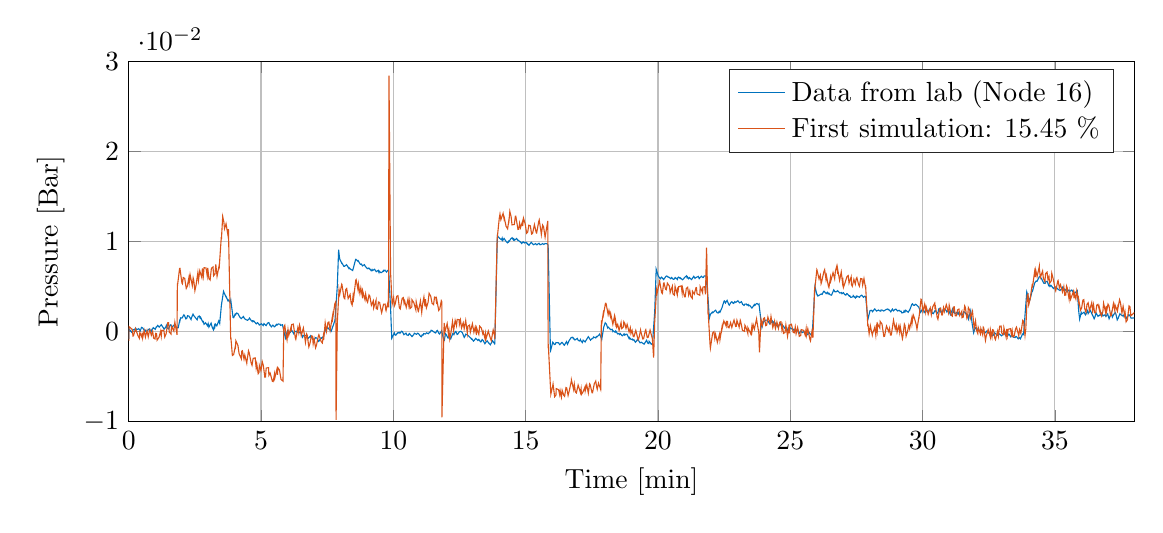
\begin{tikzpicture}

\begin{axis}[%
width=5.028in,
height=1.8in,
at={(1.011in,0.642in)},
scale only axis,
xmin=0,
xmax=38,
xlabel={Time [min]},
xmajorgrids,
ymin=-0.01,
ymax=0.03,
ylabel={Pressure [Bar]},
ymajorgrids,
axis background/.style={fill=white},
%title style={font=\bfseries},
%title={Node 16},
legend style={legend cell align=left,align=left,draw=white!15!black}
]
\addplot [color=mycolor1,solid]
  table[row sep=crcr]{%
0.000833333333333333	-0.000818830449657984\\
0.01	0.000293887047898234\\
0.1175	-9.23886119253287e-05\\
0.169166666666667	0.000219937878788601\\
0.210833333333333	0.000186878250245617\\
0.2625	0.000377406109482642\\
0.264166666666667	0.000367836217009684\\
0.299166666666667	0.000196448142718311\\
0.3775	0.000322596725318952\\
0.438333333333333	9.4659286412252e-05\\
0.439166666666667	9.55292766370991e-05\\
0.483333333333333	0.000466145112413094\\
0.526666666666667	0.000411335728248516\\
0.6	8.59593841614631e-05\\
0.620833333333333	0.000161648533720929\\
0.650833333333333	7.00342130108278e-07\\
0.701666666666667	9.46592864151802e-05\\
0.776666666666667	0.000296497018571928\\
0.85	-6.25957966753077e-06\\
0.876666666666667	0.000227767790811531\\
0.883333333333333	0.000213847947213922\\
0.929166666666667	0.000433955474096637\\
1.0025	0.000246037585530212\\
1.04083333333333	0.000508774633428327\\
1.05166666666667	0.00049659477028112\\
1.09666666666667	0.000683642668622086\\
1.15083333333333	0.00049137482893262\\
1.22416666666667	0.000736712072337692\\
1.23083333333333	0.000758461827959814\\
1.315	0.000383496041056516\\
1.3375	0.000265177370478445\\
1.4025	0.00050007473118438\\
1.42166666666667	0.000679292717497448\\
1.44583333333333	0.000410465738022517\\
1.50416666666667	0.00029388704789679\\
1.56916666666667	0.000735842082110638\\
1.58833333333333	0.000749761925708414\\
1.64416666666667	0.000494854789829843\\
1.73	0.000783691544478812\\
1.7525	0.0005748938905175\\
1.76833333333333	0.000582723802542554\\
1.81333333333333	0.000423515591397861\\
1.86916666666667	0.00040698577712317\\
1.9275	0.00121868665688969\\
1.93583333333333	0.00117431715542442\\
1.95833333333333	0.0015223132453578\\
2.015	0.00149273357771525\\
2.08416666666667	0.00185986945259277\\
2.1125	0.00174242077223963\\
2.16166666666667	0.00140573455522568\\
2.19583333333333	0.00148316368523678\\
2.2225	0.00175460063538292\\
2.2775	0.00171806104594094\\
2.35583333333333	0.001337875317687\\
2.365	0.00148664364613293\\
2.42916666666667	0.0019312086510244\\
2.455	0.00178853025415546\\
2.54	0.00146837385141052\\
2.58583333333333	0.00130307570869914\\
2.62333333333333	0.00166151168132597\\
2.66666666666667	0.00172676094818454\\
2.69916666666667	0.00148577365591192\\
2.71583333333333	0.00158234257086928\\
2.7975	0.00107513826979937\\
2.81833333333333	0.00112211774193623\\
2.8475	0.000806311290324796\\
2.90416666666667	0.000979439345066571\\
2.97666666666667	0.000645363098723498\\
3.0025	0.000882870430102087\\
3.03083333333333	0.000490504838704844\\
3.11416666666667	0.000935069843604142\\
3.15333333333333	0.000495724780057966\\
3.2	0.000198188123164703\\
3.24	0.00064362311828145\\
3.2525	0.000492244819158966\\
3.27583333333333	0.000827191055720933\\
3.32833333333333	0.000640143157386711\\
3.40083333333333	0.00117605713587818\\
3.43833333333333	0.000898530254160729\\
3.50333333333333	0.00295170718474833\\
3.58333333333333	0.00446114022481266\\
3.59083333333333	0.00440372086997454\\
3.67416666666667	0.00386084696968721\\
3.68083333333333	0.00388607668620619\\
3.7525	0.00340062214076409\\
3.78	0.00350763093841419\\
3.835	0.00321009428153159\\
3.85666666666667	0.00350067101661904\\
3.94166666666667	0.00158234257086644\\
3.96666666666667	0.00153797306939833\\
4.02083333333333	0.00193468861192482\\
4.0375	0.00186334941348573\\
4.08	0.00205474726294778\\
4.12583333333333	0.00199384794721565\\
4.20416666666667	0.0015849525415423\\
4.2525	0.00142835430107521\\
4.335	0.00166586163244954\\
4.37916666666667	0.00142835430105888\\
4.44666666666667	0.0012995957477774\\
4.49416666666667	0.00124826632450988\\
4.54916666666667	0.00140747453566274\\
4.56583333333333	0.00149708352882283\\
4.64166666666667	0.00116735723360546\\
4.68166666666667	0.00120389682304745\\
4.6925	0.00108731813291496\\
4.72916666666667	0.0011708371944938\\
4.81666666666667	0.000865470625572975\\
4.82166666666667	0.000854160752647146\\
4.86583333333333	0.000979439345028199\\
4.90583333333333	0.00086982057670508\\
4.935	0.000726272189605873\\
5.0175	0.00086547062557725\\
5.07916666666667	0.000666242864091199\\
5.11166666666667	0.000879390469178926\\
5.19416666666667	0.000660152932531272\\
5.245	0.000934199853337647\\
5.295	0.000997709139761979\\
5.335	0.000725402199396222\\
5.34333333333333	0.000740192033223189\\
5.39	0.000522694476999111\\
5.44833333333333	0.000712352346008457\\
5.50166666666667	0.000526174437908769\\
5.51833333333333	0.000536614320612153\\
5.58166666666667	0.000794131427158049\\
5.60666666666667	0.000721052248262702\\
5.64666666666667	0.000850680791750283\\
5.71833333333333	0.00080892126096796\\
5.7375	0.000686252639269871\\
5.81083333333333	0.000755851857261236\\
5.8675	-8.86955034747061e-06\\
5.92166666666667	-0.000715301612902008\\
5.96333333333333	-0.000247246871955611\\
6.005	0.000114669061558853\\
6.04416666666667	4.50698435660729e-05\\
6.08583333333333	-0.000145458015660044\\
6.16166666666667	0.000132068866061666\\
6.2175	-0.000125448240488477\\
6.2275	-0.000227237096791164\\
6.28083333333333	-1.03963834408027e-06\\
6.35083333333333	3.28899804277333e-05\\
6.36416666666667	-7.32488269914039e-05\\
6.43083333333333	-4.80191104581945e-05\\
6.46166666666667	-0.00012805821114302\\
6.48916666666667	-6.10689638360223e-05\\
6.56833333333333	-0.000572623216029508\\
6.5725	-0.000622212658843643\\
6.605	-0.000434294770290541\\
6.72	-0.000429074828935991\\
6.74333333333333	-0.00058045312805706\\
6.74583333333333	-0.000570883235583214\\
6.78916666666667	-0.000747491251216162\\
6.8725	-0.00046822438905951\\
6.88833333333333	-0.000698771798631578\\
6.9275	-0.000669192130986179\\
6.96083333333333	-0.000862329960892402\\
7.02416666666667	-0.000852760068411437\\
7.0625	-0.00067615205278275\\
7.10583333333333	-0.000717911583587805\\
7.175	-0.00109809731181616\\
7.19	-0.00106329770282475\\
7.26833333333333	-0.000690941886611146\\
7.29083333333333	-0.00075358118279599\\
7.35583333333333	-0.000554353421315629\\
7.4425	0.00026952732157963\\
7.44583333333333	0.000235597702809232\\
7.52	0.000442655376314285\\
7.53166666666667	0.000393065933507269\\
7.61833333333333	0.000119019012683852\\
7.6525	2.85400293027482e-05\\
7.70583333333333	0.000496594770271877\\
7.79	0.00122303660799372\\
7.79333333333333	0.00121346671551988\\
7.88166666666667	0.00499183426196237\\
7.9325	0.0090920981915819\\
7.96916666666667	0.00809856935482327\\
8.05166666666667	0.00757570522971247\\
8.06166666666667	0.00759745498533317\\
8.13083333333333	0.00724597893451499\\
8.15666666666667	0.00725728880743515\\
8.23166666666667	0.00742432693060135\\
8.2325	0.00742606691105049\\
8.31916666666667	0.0070171715054077\\
8.3275	0.00709547062564053\\
8.3875	0.00691712262953144\\
8.46333333333333	0.00678488411536944\\
8.49416666666667	0.00710939046921948\\
8.57583333333333	0.00802636016616599\\
8.58333333333333	0.00803332008796827\\
8.65583333333333	0.00781843250243708\\
8.66916666666667	0.00787672184749692\\
8.75416666666667	0.0074652164711726\\
8.79583333333333	0.00749914608993589\\
8.8325	0.00729556837732059\\
8.9075	0.00743389682304819\\
8.93166666666667	0.00728077854345241\\
9.01916666666667	0.00698585185727763\\
9.07416666666667	0.00706415097747919\\
9.09166666666667	0.0069545322091447\\
9.10666666666667	0.0069780219452046\\
9.16333333333333	0.00675617443789389\\
9.19666666666667	0.0069014628054536\\
9.2175	0.00677966417397653\\
9.29083333333333	0.00692147258061238\\
9.35416666666667	0.00664742565979037\\
9.43	0.00679967394912108\\
9.45666666666667	0.0065708665199939\\
9.46833333333333	0.00671789486798713\\
9.5225	0.00655433670576468\\
9.55166666666667	0.00654302683282464\\
9.62666666666667	0.00677618421306687\\
9.635	0.00670919496577409\\
9.68166666666667	0.00682316368521226\\
9.7425	0.00661523602149469\\
9.7875	0.00678836407622367\\
9.825	0.0067161548875735\\
9.895	0.00262720083088408\\
9.94	-0.000746621260995145\\
10.0383333333333	-0.000151547947174493\\
10.065	-0.000379485386107659\\
10.0916666666667	-0.000408195063541991\\
10.15	-0.000171557722381574\\
10.1625	-0.000212447262944296\\
10.2166666666667	-7.41188172038998e-05\\
10.2516666666667	-0.000187217546445198\\
10.31	3.46299609195189e-05\\
10.3391666666667	-5.38958941508072e-06\\
10.3975	-0.000348165738031578\\
10.4775	-0.000174167693031843\\
10.5075	-0.000370785483840619\\
10.5608333333333	-0.000428204838689397\\
10.5941666666667	-0.000255946774185709\\
10.605	-0.000219407184738035\\
10.6833333333333	-0.00048040425219216\\
10.7066666666667	-0.000557833382211076\\
10.7708333333333	-0.000337725855322504\\
10.7941666666667	-0.000181997605050874\\
10.8775	-0.000305536217012611\\
10.9141666666667	-0.000186347556168753\\
10.9466666666667	-0.000216797214042289\\
11.0316666666667	-0.000538693597277581\\
11.0616666666667	-0.000576103176924955\\
11.0891666666667	-0.000369045503392895\\
11.1208333333333	-0.00040558509284909\\
11.145	-0.000222017155416726\\
11.2083333333333	-0.000281176490707538\\
11.2525	-0.000141108064471096\\
11.3233333333333	-0.000238546969645939\\
11.3833333333333	-3.49692570064813e-05\\
11.3983333333333	-4.80191103885697e-05\\
11.43	0.000148598680405995\\
11.4733333333333	8.59593842197359e-05\\
11.5566666666667	-0.000100218523916909\\
11.5983333333333	-0.000158507868990965\\
11.6391666666667	7.11695503558124e-05\\
11.6658333333333	0.000130328885652314\\
11.7208333333333	-0.00020983729226845\\
11.7475	-0.00026986661779875\\
11.8216666666667	6.94295699194686e-05\\
11.8258333333333	8.85693548700051e-05\\
11.905	-0.000969338758559563\\
11.9258333333333	-0.000985868572828563\\
11.97	-0.000239416959925229\\
11.9966666666667	-0.000329025953075365\\
12.065	-0.000723131524952292\\
12.1333333333333	-0.000652662316698693\\
12.1675	-0.000818830449648145\\
12.1716666666667	-0.000784030840659575\\
12.2483333333333	-0.000214187243428962\\
12.2891666666667	-0.000343815786916543\\
12.345	1.28802053130234e-05\\
12.3633333333333	2.15801075686972e-05\\
12.4108333333333	-0.000324676001943261\\
12.4383333333333	-0.000276826539603856\\
12.4941666666667	-2.01794232647795e-05\\
12.5533333333333	3.63699413558766e-05\\
12.6091666666667	-0.000131538172029932\\
12.6791666666667	-0.000650052346028537\\
12.7091666666667	-0.000504763978485867\\
12.7325	-0.000295096334306383\\
12.7983333333333	-0.000374265444767333\\
12.8716666666667	-0.000565663294227248\\
12.9575	-0.000841450195516874\\
12.9658333333333	-0.000804910606074891\\
13.0275	-0.00106155772241112\\
13.0508333333333	-0.00100500835778194\\
13.1116666666667	-0.00075793113392951\\
13.1416666666667	-0.000842320185773418\\
13.1908333333333	-0.000992828494716089\\
13.23	-0.000871029863204906\\
13.295	-0.00115116671557547\\
13.3141666666667	-0.00113724687197095\\
13.355	-0.000883209726316239\\
13.4025	-0.00103893797657366\\
13.46	-0.00135474442816662\\
13.485	-0.00123207580646426\\
13.5458333333333	-0.00102849809386174\\
13.5791666666667	-0.00118422634410212\\
13.6591666666667	-0.00144783338224345\\
13.665	-0.00146871314764173\\
13.7475	-0.00101805821116403\\
13.8308333333333	-0.00137475420337939\\
13.835	-0.0013434345552891\\
13.9225	0.00968456153468407\\
13.9333333333333	0.0106302409090891\\
14.0133333333333	0.0103579339686892\\
14.0875	0.0101978557673281\\
14.1116666666667	0.0103875136363147\\
14.1325	0.010121296627526\\
14.185	0.0103431441348623\\
14.2683333333333	0.00998731813292619\\
14.315	0.00986377952098717\\
14.3475	0.0100290776637199\\
14.36	0.00995860845552311\\
14.445	0.0103196543988137\\
14.4883333333333	0.0104240532257823\\
14.5325	0.0101935058162102\\
14.5516666666667	0.0102996446236436\\
14.5733333333333	0.0101369564516038\\
14.6591666666667	0.010337924193502\\
14.7041666666667	0.0101421763929299\\
14.7125	0.0101587062072103\\
14.7983333333333	0.00994729858259444\\
14.8041666666667	0.00996469838710294\\
14.845	0.00979244032260208\\
14.9058333333333	0.00996817834798987\\
14.9508333333333	0.00984115977518098\\
15.0091666666667	0.00992467883673424\\
15.0575	0.00975590073314589\\
15.0608333333333	0.00979766026393673\\
15.1258333333333	0.00958364266866493\\
15.1491666666667	0.00968282155426477\\
15.2116666666667	0.00991249897361723\\
15.2358333333333	0.00982636994135401\\
15.2958333333333	0.00964889193548157\\
15.38	0.00977330053763734\\
15.4075	0.0096497619257097\\
15.4241666666667	0.00963236212120688\\
15.4916666666667	0.00979418030302992\\
15.5075	0.00980723015639211\\
15.545	0.00964019203321169\\
15.5875	0.00967934159335794\\
15.6383333333333	0.00977330053765155\\
15.685	0.00968282155425908\\
15.7358333333333	0.00977765048873533\\
15.8016666666667	0.00976895058649671\\
15.8491666666667	0.00962366221895973\\
15.9366666666667	-0.00215513543500907\\
15.9383333333333	-0.00216731529816304\\
16.0233333333333	-0.00117117649076266\\
16.0241666666667	-0.00117378646143851\\
16.0816666666667	-0.00143739349955711\\
16.1116666666667	-0.00142434364617219\\
16.1458333333333	-0.00122424589445945\\
16.245	-0.00125034560121225\\
16.2833333333333	-0.00145392331379771\\
16.2891666666667	-0.00146349320626445\\
16.3641666666667	-0.00120858607040435\\
16.3791666666667	-0.00120945606064669\\
16.4608333333333	-0.00153396241450099\\
16.4616666666667	-0.00153309242427571\\
16.5416666666667	-0.00111984706744823\\
16.5816666666667	-0.00141042380255345\\
16.6366666666667	-0.00103284804497394\\
16.7175	-0.000671802101683341\\
16.7775	-0.000630912561083677\\
16.8	-0.000794470723368648\\
16.8125	-0.000753581182803095\\
16.8608333333333	-0.000937149120246825\\
16.9533333333333	-0.000765761045968413\\
16.9866666666667	-0.000986738563048165\\
17.0433333333333	-0.00105111783969636\\
17.0683333333333	-0.000896259579692638\\
17.075	-0.00096324882699679\\
17.1416666666667	-0.00121902595309638\\
17.1733333333333	-0.000959768866112709\\
17.2466666666667	-0.00114942673508796\\
17.2508333333333	-0.00112680698924482\\
17.3283333333333	-0.000755321163247974\\
17.3683333333333	-0.000571753225781499\\
17.425	-0.0008327502932612\\
17.4508333333333	-0.000961508846549067\\
17.5108333333333	-0.000774460948192821\\
17.5366666666667	-0.000789250781988535\\
17.5666666666667	-0.000602202883635133\\
17.6491666666667	-0.000710081671590104\\
17.6708333333333	-0.000552613440876426\\
17.695	-0.000600462903255619\\
17.775	-0.000364695552263636\\
17.795	-0.000281176490673427\\
17.8616666666667	-0.000753581182757618\\
17.875	-0.000878859775144347\\
17.95	0.000483544916901169\\
18.005	0.000980309335350107\\
18.0491666666667	0.000842850879812257\\
18.1008333333333	0.000403505816214927\\
18.125	0.000487024877842093\\
18.2116666666667	0.000206018035178029\\
18.2691666666667	0.000247777565980239\\
18.2916666666667	2.76700391087237e-05\\
18.3033333333333	8.76993645850394e-05\\
18.3825	-7.41188172607432e-05\\
18.405	6.8559579634489e-05\\
18.4758333333333	-0.000260296725329165\\
18.5175	-0.000221147165225546\\
18.55	-0.000331635923756887\\
18.5758333333333	-0.000219407184780668\\
18.6375	-0.000443864662767232\\
18.6608333333333	-0.000472574340127666\\
18.7191666666667	-0.000259426735103888\\
18.7433333333333	-0.000396015200365293\\
18.7975	-0.000288136412566642\\
18.8258333333333	-0.000295096334380282\\
18.9083333333333	-0.000776200928597912\\
18.9216666666667	-0.000663102199379359\\
18.985	-0.000886689687061057\\
19.0375	-0.00083101031269979\\
19.0541666666667	-0.000966728787787072\\
19.09	-0.000908439442681749\\
19.1458333333333	-0.00119031627554836\\
19.1758333333333	-0.00109983729215304\\
19.2241666666667	-0.000888429667522991\\
19.27	-0.00101718822083074\\
19.3241666666667	-0.00125295557173462\\
19.3733333333333	-0.00118944628533445\\
19.4383333333333	-0.00132081480937489\\
19.4758333333333	-0.00140259389053443\\
19.5258333333333	-0.00116421656884672\\
19.57	-0.000975428689994437\\
19.6116666666667	-0.00127731529798569\\
19.6525	-0.00133995459418333\\
19.6658333333333	-0.00108417746808658\\
19.7025	-0.00121206603120316\\
19.7483333333333	-0.00141651373401959\\
19.7933333333333	-0.00133821461376686\\
19.8766666666667	0.00219742565996381\\
19.9325	0.00691973260020728\\
20.0116666666667	0.00617241099696213\\
20.0516666666667	0.00599232302047067\\
20.0941666666667	0.00586704442818342\\
20.1308333333333	0.00604278245348593\\
20.1458333333333	0.0060192927174374\\
20.2141666666667	0.00577395547411226\\
20.2291666666667	0.00584007473113712\\
20.305	0.0061471812804403\\
20.33	0.00618111089921496\\
20.385	0.00604539242420725\\
20.4016666666667	0.00606888216028989\\
20.4791666666667	0.00587313435973766\\
20.515	0.006008852834734\\
20.5691666666667	0.00582180493644598\\
20.6025	0.00580440513196305\\
20.6508333333333	0.00600363289345052\\
20.7341666666667	0.00578178538616254\\
20.75	0.00598275312803236\\
20.7775	0.00605409232643735\\
20.8391666666667	0.00590967394912564\\
20.8458333333333	0.00596361334306476\\
20.9166666666667	0.00577656544481084\\
20.9316666666667	0.00575046573802962\\
21.015	0.00602886260995529\\
21.0775	0.00618807082100585\\
21.1	0.00598710307917014\\
21.1175	0.00606975215053791\\
21.1558333333333	0.00586965439885927\\
21.1908333333333	0.00599754296184511\\
21.2675	0.00576960552300858\\
21.2775	0.0058096250733318\\
21.3525	0.00613761138804177\\
21.3991666666667	0.00590880395892879\\
21.4491666666667	0.00603843250240499\\
21.4591666666667	0.0060271226295161\\
21.5233333333333	0.00613500141736591\\
21.5575	0.00588879418379275\\
21.6266666666667	0.00611151168126053\\
21.6366666666667	0.00614631129023775\\
21.6975	0.00599841295207039\\
21.7183333333333	0.00602451265881183\\
21.7483333333333	0.00618546085036979\\
21.8141666666667	0.00618111089928317\\
21.89	0.00378080786897823\\
21.94	0.00145967394912856\\
21.9775	0.0018937990712264\\
22.055	0.00216436603118705\\
22.0733333333333	0.00208954687186957\\
22.1525	0.00230878440851012\\
22.18	0.00236794374380093\\
22.2316666666667	0.00210520669593035\\
22.2741666666667	0.00205561725307786\\
22.3175	0.00225397502423204\\
22.3425	0.0021426162754072\\
22.4158333333333	0.00262807082108663\\
22.495	0.00336843250254656\\
22.5166666666667	0.00339975215070222\\
22.55	0.00317877463362816\\
22.6116666666667	0.00345804149577345\\
22.6783333333333	0.00299172673518097\\
22.695	0.00293082741942254\\
22.7658333333333	0.00327708352900555\\
22.7891666666667	0.00331101314775747\\
22.8475	0.00313788509300576\\
22.8608333333333	0.00312309525916458\\
22.9008333333333	0.0033258029816555\\
22.9408333333333	0.0032405439396062\\
23.0208333333333	0.00342759183788854\\
23.0283333333333	0.00337104247325652\\
23.0916666666667	0.0031926944770849\\
23.1533333333333	0.00331797306957111\\
23.2016666666667	0.00300999652995738\\
23.2533333333333	0.00290211774202231\\
23.2808333333333	0.00304392614873206\\
23.3375	0.00305871598255049\\
23.3658333333333	0.00293778734124754\\
23.4091666666667	0.00301086652017131\\
23.4216666666667	0.00286383817212123\\
23.4658333333333	0.00291168763450042\\
23.5508333333333	0.00260197111433381\\
23.5533333333333	0.00260545107523495\\
23.6416666666667	0.00300303660813239\\
23.6608333333333	0.00290472771268679\\
23.7175	0.00309699555242883\\
23.7441666666667	0.00311874530807228\\
23.8083333333333	0.00296910698935204\\
23.8191666666667	0.0030239163735335\\
23.9041666666667	0.000893310312878662\\
23.9283333333333	0.00046005518094358\\
23.9891666666667	0.00108122820152841\\
23.9916666666667	0.00107426827974319\\
24.0691666666667	0.00126827609978232\\
24.1266666666667	0.00126044618777751\\
24.1566666666667	0.00110993787888315\\
24.1675	0.00112559770294962\\
24.2225	0.000845460850556326\\
24.3233333333333	0.00116039731185293\\
24.3416666666667	0.000945509726338792\\
24.3641666666667	0.00104729858267416\\
24.4116666666667	0.000783691544572598\\
24.4333333333333	0.000908970136979229\\
24.4808333333333	0.000680162707763943\\
24.5341666666667	0.000513994574746282\\
24.57	0.000692342570878107\\
24.6233333333333	0.000869820576818767\\
24.675	0.000540964271821001\\
24.7408333333333	0.000619263392016872\\
24.7791666666667	0.000385236021483992\\
24.8058333333333	0.000423515591362333\\
24.84	0.000258217448581316\\
24.8691666666667	0.000385236021438515\\
24.89	0.000119889002875032\\
24.9741666666667	0.000453965249247235\\
25.0408333333333	0.000307806891467921\\
25.0466666666667	0.00032346671552301\\
25.13	0.000161648533722705\\
25.1391666666667	0.000236467693051565\\
25.2025	5.55097262609355e-05\\
25.28	0.000227767790776004\\
25.3033333333333	-0.000106308455499568\\
25.34	-0.000197657429171327\\
25.3875	6.07296675785296e-05\\
25.4025	8.07394427429775e-05\\
25.4458333333333	-0.000123708260045027\\
25.5108333333333	-4.51959924947787e-06\\
25.555	-0.000218537194566756\\
25.5908333333333	-8.28187194567287e-05\\
25.6533333333333	-0.000351645698898603\\
25.6591666666667	-0.000346425757569643\\
25.7166666666667	-0.000109788416440493\\
25.7425	-0.000214187243377809\\
25.7991666666667	-0.000408195063519259\\
25.8308333333333	-0.000242896920868985\\
25.9175	0.00427148235582746\\
25.9325	0.0049796543988553\\
26.005	0.00411401412514789\\
26.0158333333333	0.00412706397849871\\
26.0416666666667	0.0039469760019902\\
26.0983333333333	0.00404354491691135\\
26.1725	0.00418274335291113\\
26.2025	0.00412793396874674\\
26.2608333333333	0.00446462018569815\\
26.2758333333333	0.00448201999020949\\
26.3558333333333	0.00420971304991764\\
26.4	0.00435239144673898\\
26.4291666666667	0.00418361334311368\\
26.4575	0.00426800239487517\\
26.5025	0.00408965439883997\\
26.5591666666667	0.00404093494624687\\
26.6166666666667	0.00445331031281494\\
26.6425	0.00463078831867034\\
26.685	0.00441590073309368\\
26.7325	0.00441764071355562\\
26.7883333333333	0.00454117932550031\\
26.7933333333333	0.00450724970671997\\
26.8758333333333	0.00427235234605843\\
26.9266666666667	0.0043367316226043\\
26.9533333333333	0.00420101314752838\\
27.005	0.00432281177902251\\
27.0516666666667	0.00411749408602628\\
27.0975	0.00404963484856791\\
27.1325	0.00421580298142073\\
27.1533333333333	0.0041949232159912\\
27.2308333333333	0.00393392614861096\\
27.25	0.00396872575759954\\
27.285	0.00379646769312426\\
27.3633333333333	0.00385910698927074\\
27.3783333333333	0.003998305425208\\
27.4575	0.00372773846536671\\
27.4925	0.00392522624639224\\
27.5116666666667	0.00384518714578559\\
27.5325	0.00392783621711924\\
27.6141666666667	0.00380516759532025\\
27.6441666666667	0.00394436603131436\\
27.7	0.00404354491689997\\
27.7566666666667	0.00383648724345886\\
27.765	0.00380603758559102\\
27.8125	0.00392957619744476\\
27.8483333333333	0.00388868665684509\\
27.9316666666667	0.00135440513192617\\
27.9341666666667	0.00134831520034918\\
28.0125	0.00232792419338108\\
28.0666666666667	0.00236098382194183\\
28.1066666666667	0.00221656544461309\\
28.1075	0.0022104755130361\\
28.19	0.00251410210155752\\
28.1941666666667	0.00250192223840355\\
28.26	0.00227398479950448\\
28.3383333333333	0.00239752341143214\\
28.365	0.00231139437915755\\
28.4175	0.00226876485810731\\
28.43	0.00239056348959008\\
28.4833333333333	0.00238621353846366\\
28.5166666666667	0.00228616466260161\\
28.545	0.00230878440845896\\
28.6283333333333	0.00245755273694823\\
28.6825	0.00250627218952996\\
28.7016666666667	0.00242449310837611\\
28.7191666666667	0.00245233279558517\\
28.7983333333333	0.00219307570858729\\
28.8066666666667	0.00223918519051022\\
28.8575	0.00249496231661266\\
28.8975	0.00230008450619476\\
28.9725	0.00249061236550897\\
28.9916666666667	0.00249148235574563\\
29.055	0.00228355469199397\\
29.11	0.002366203763339\\
29.1575	0.00224962507316247\\
29.1875	0.00226354491673288\\
29.2083333333333	0.00208171695977381\\
29.2775	0.00210433670571075\\
29.3025	0.00230965439876382\\
29.3325	0.00218089584545038\\
29.3608333333333	0.00236533377310234\\
29.455	0.00214348626571205\\
29.5066666666667	0.00238969349938753\\
29.5108333333333	0.00238534354827248\\
29.595	0.00303087629536418\\
29.6191666666667	0.00308394569910643\\
29.6508333333333	0.00292908743901744\\
29.6925	0.00291777756599783\\
29.7333333333333	0.00303522624641102\\
29.775	0.00294996720440151\\
29.8575	0.00269332008795442\\
29.925	0.00213304638315645\\
29.945	0.00222787531769524\\
30.0091666666667	0.00261676094815226\\
30.0325	0.00239056348966966\\
30.0608333333333	0.00211390659816613\\
30.13	0.00236533377314782\\
30.1925	0.00213826632439447\\
30.2133333333333	0.0021808958454788\\
30.2633333333333	0.00251845205274077\\
30.3008333333333	0.0025062721895186\\
30.375	0.00201820767338501\\
30.4025	0.00198079809377742\\
30.4683333333333	0.00232792419348339\\
30.4866666666667	0.00235315390997112\\
30.5233333333333	0.00211303660795222\\
30.575	0.00204169740955291\\
30.61	0.00251323211145728\\
30.6591666666667	0.0026028411045932\\
30.6925	0.00214000630495871\\
30.7516666666667	0.00223135527853384\\
30.775	0.00242188313775711\\
30.8641666666667	0.00243319301064031\\
30.9083333333333	0.0022504950634389\\
30.9175	0.00217480591385634\\
30.98	0.00238273357766484\\
30.9958333333333	0.00228964462364485\\
31.0508333333333	0.00188335918856848\\
31.1325	0.00250627218956408\\
31.165	0.00218002585519668\\
31.1741666666667	0.00223657521982869\\
31.2258333333333	0.00199471793738194\\
31.3075	0.00214348626578027\\
31.3266666666667	0.00198340806442485\\
31.3491666666667	0.00209389682297893\\
31.3716666666667	0.00189553905172243\\
31.4558333333333	0.00202255762460236\\
31.4816666666667	0.00183985967731001\\
31.5216666666667	0.00194947844563882\\
31.5533333333333	0.00220960552285629\\
31.6091666666667	0.00209389682298462\\
31.67	0.00178940024432318\\
31.7008333333333	0.0018868391494696\\
31.7325	0.00140225459432809\\
31.8166666666667	0.00233488411526292\\
31.8716666666667	0.000888960361678362\\
31.9291666666667	-0.000135888123153502\\
31.9866666666667	0.000437435435012332\\
32.0458333333333	0.000274747262884428\\
32.0825	0.000293017057626743\\
32.1333333333333	3.63699413331309e-05\\
32.1341666666667	3.9849902234268e-05\\
32.195	0.000240817644155247\\
32.2258333333333	0.000203408064479452\\
32.3091666666667	2.59300584990046e-05\\
32.3508333333333	-0.000176777663844122\\
32.4375	7.55195014253834e-05\\
32.4816666666667	-0.000115008357803564\\
32.4858333333333	-7.41188172152657e-05\\
32.5716666666667	-0.000220277174977523\\
32.58	-0.000151547947225647\\
32.6258333333333	-0.000464744428100114\\
32.6741666666667	-0.000400365151497398\\
32.7225	-0.000132408162309222\\
32.7491666666667	-0.000212447262978407\\
32.8208333333333	-0.000436034750705569\\
32.8375	-0.000394275219960202\\
32.8841666666667	-0.000233327028356767\\
32.925	-0.00032641598238814\\
32.9841666666667	-0.00047518431078078\\
33.0183333333333	-0.000380355376264727\\
33.0616666666667	-0.00016981774193385\\
33.11	-0.000307276197500136\\
33.1725	-0.00052651373405542\\
33.2041666666667	-0.000504763978434714\\
33.2591666666667	-0.000279436510302447\\
33.2891666666667	-0.000378615395916479\\
33.3208333333333	-0.000576103176896534\\
33.3608333333333	-0.000446474633420332\\
33.4425	-0.000645702394856645\\
33.4983333333333	-0.000659622238410013\\
33.5266666666667	-0.000529993694967909\\
33.5391666666667	-0.000529993694967909\\
33.6116666666667	-0.000811870527754929\\
33.6575	-0.000661362218889003\\
33.695	-0.000804040615750123\\
33.7116666666667	-0.000693551857230149\\
33.7783333333333	-0.000270736608060984\\
33.8158333333333	-0.000340335826026772\\
33.885	0.00242449310852959\\
33.9358333333333	0.00439676094827388\\
34.0316666666667	0.00347196133933249\\
34.055	0.00359375997076979\\
34.06	0.00357114022495221\\
34.1433333333333	0.00455161920815254\\
34.1558333333333	0.00452290953071252\\
34.2358333333333	0.00540507961884241\\
34.2908333333333	0.00561213729232332\\
34.3233333333333	0.00558342761494583\\
34.4108333333333	0.00609933181814068\\
34.4308333333333	0.00614022135866077\\
34.4983333333333	0.0058505146139201\\
34.5791666666667	0.0053720199902703\\
34.6283333333333	0.0053502702346496\\
34.66	0.00556341783982117\\
34.7108333333333	0.00555645791804164\\
34.7608333333333	0.0051371226295235\\
34.775	0.00520498186710694\\
34.8133333333333	0.00500053416424504\\
34.8483333333333	0.00514669252209256\\
34.9358333333333	0.00480739633428907\\
34.9425	0.00477694667641555\\
35.0058333333333	0.0049552946725758\\
35.0266666666667	0.00496399457478315\\
35.1108333333333	0.00471778734106221\\
35.1916666666667	0.0045542291787886\\
35.1983333333333	0.00458293885622293\\
35.2858333333333	0.0048769955522435\\
35.29	0.0049074452101284\\
35.3258333333333	0.00468124775166853\\
35.3733333333333	0.00471865733140117\\
35.4575	0.00441764071347603\\
35.4616666666667	0.00444287043000924\\
35.525	0.00460642859232831\\
35.56	0.00445766026380494\\
35.6366666666667	0.00460816857272203\\
35.6383333333333	0.00461512849452429\\
35.7216666666667	0.00421493299113292\\
35.7358333333333	0.00423146280537919\\
35.8116666666667	0.00444983035182855\\
35.8441666666667	0.00453943934497016\\
35.8991666666667	0.00225832497555171\\
35.9341666666667	0.0013805048387074\\
35.9933333333333	0.00211999652984542\\
36.0125	0.00196078831877212\\
36.0991666666667	0.00214870620734228\\
36.1533333333333	0.00185116955031828\\
36.1616666666667	0.00189118910066992\\
36.2375	0.00234097404706728\\
36.2566666666667	0.0019955879276925\\
36.3366666666667	0.0023479339688468\\
36.3383333333333	0.0023522839199789\\
36.4183333333333	0.00181984990229904\\
36.4241666666667	0.00183202976540753\\
36.4825	0.00141878440854026\\
36.5166666666667	0.00164498186702286\\
36.5533333333333	0.00208171695997846\\
36.6266666666667	0.00169370131961596\\
36.6841666666667	0.00183202976545301\\
36.6975	0.00178157033232974\\
36.775	0.00207475703823302\\
36.7791666666667	0.002093896823212\\
36.815	0.00172937091890372\\
36.8941666666667	0.0018703093353086\\
36.9258333333333	0.00167543152486797\\
36.9925	0.00195904833832157\\
37.0375	0.00151883328445347\\
37.0466666666667	0.00142139437927864\\
37.125	0.00199210796674588\\
37.1308333333333	0.00207475703811934\\
37.1708333333333	0.0016032223363457\\
37.2133333333333	0.0018572594820601\\
37.2783333333333	0.0021130366081\\
37.3025	0.00195991832845022\\
37.3541666666667	0.00129437580642144\\
37.3875	0.00146228391988398\\
37.4558333333333	0.00197905811349738\\
37.475	0.00190771891499009\\
37.5558333333333	0.0017415507819781\\
37.6008333333333	0.00183637971648277\\
37.6108333333333	0.00166238167152852\\
37.6516666666667	0.00178853025415475\\
37.7075	0.00147011383183764\\
37.7375	0.00159539242431248\\
37.7933333333333	0.00189292908115458\\
37.8366666666667	0.00173198088955115\\
37.8808333333333	0.00148577365590409\\
38	0.0015205732648131\\
};
\addlegendentry{Data from lab (Node 16)};

\addplot [color=mycolor2,solid]
  table[row sep=crcr]{%
0.000833333333333333	-0.00102189496608339\\
0.0108333333333333	0.000549560591616079\\
0.130833333333333	0.000244254857973151\\
0.1625	-0.000501906144537622\\
0.18	-0.000470814330594456\\
0.256666666666667	0.000319322455360866\\
0.271666666666667	0.000177722624725499\\
0.350833333333333	-0.00046069129716403\\
0.404166666666667	-0.000754023703468938\\
0.420833333333333	-9.47678401177999e-05\\
0.508333333333333	-0.00069277567482734\\
0.511666666666667	-0.000124192776212159\\
0.529166666666667	-0.000697259346058747\\
0.585	0.000122218603805916\\
0.630833333333333	-0.000617842199229081\\
0.690833333333333	9.85168898411392e-05\\
0.738333333333333	-0.000579658673329482\\
0.785833333333333	0.000108325808511434\\
0.800833333333333	0.000198634754059528\\
0.854166666666667	-0.000418236575299922\\
0.905	1.87604941544983e-05\\
0.941666666666667	-0.000727674362704281\\
0.994166666666667	-0.000818527518904671\\
1.0175	-0.000198135281068068\\
1.0525	-0.000238053647154075\\
1.0725	-0.000956411710027101\\
1.14416666666667	-0.000646291178784121\\
1.20916666666667	6.8725759393234e-05\\
1.23083333333333	-0.000484635682437731\\
1.25166666666667	0.000109143011102175\\
1.32666666666667	0.00015903615397426\\
1.36166666666667	-0.00060791094819693\\
1.415	-0.0002421171364637\\
1.4775	0.0009989156001468\\
1.505	0.000999237529473067\\
1.53333333333333	-6.370312278827e-05\\
1.59916666666667	-0.000275173055918521\\
1.61583333333333	0.000586548966681007\\
1.705	5.10771900903305e-05\\
1.74416666666667	0.00103604228387939\\
1.8275	-0.000365784217116175\\
1.8375	0.00534083407883731\\
1.845	0.00515608536636156\\
1.9225	0.00701746022502823\\
1.93666666666667	0.00702310150496927\\
2.01083333333333	0.00538176416041336\\
2.02916666666667	0.00530464912849667\\
2.06083333333333	0.00600515994498475\\
2.11666666666667	0.00589762948390643\\
2.17416666666667	0.00479466080022386\\
2.21333333333333	0.00503402431681833\\
2.27083333333333	0.00593915799051823\\
2.28666666666667	0.00543341030806468\\
2.32	0.00630713200639701\\
2.40333333333333	0.0051012727505605\\
2.435	0.00594962349145101\\
2.45833333333333	0.00565646607003166\\
2.50083333333333	0.00454027894495633\\
2.54166666666667	0.00508537165431632\\
2.6125	0.00653424486626509\\
2.63666666666667	0.00569786205512172\\
2.685	0.00675391139053474\\
2.7625	0.00600481992204433\\
2.78333333333333	0.00700583957016677\\
2.82	0.00617283186810188\\
2.84666666666667	0.00709172089741361\\
2.92083333333333	0.0070677101930983\\
2.9675	0.00618936052809555\\
2.9875	0.00706397081784779\\
3.03166666666667	0.00586391063065979\\
3.07583333333333	0.00572356374309204\\
3.12416666666667	0.0070276278094077\\
3.18666666666667	0.00717930166271188\\
3.2075	0.00618723564434362\\
3.26083333333333	0.00639963831924542\\
3.29083333333333	0.00746724159348718\\
3.33833333333333	0.00613683047593819\\
3.41333333333333	0.00729385081646232\\
3.41583333333333	0.0069243689488357\\
3.49833333333333	0.0104822549971946\\
3.50333333333333	0.0102494197357017\\
3.55166666666667	0.0127833575094516\\
3.59666666666667	0.0121463531310316\\
3.62	0.0114299923754679\\
3.67833333333333	0.0119690523125914\\
3.75583333333333	0.010597665319141\\
3.76833333333333	0.0113894683847649\\
3.85333333333333	-0.000832085942506738\\
3.85916666666667	-0.00061656727847624\\
3.9175	-0.00265766467403693\\
3.96583333333333	-0.0025633260521799\\
4.02416666666667	-0.00171019511857237\\
4.02916666666667	-0.00194044701325533\\
4.04916666666667	-0.00103349605698537\\
4.12833333333333	-0.00155734955504853\\
4.17083333333333	-0.00245273105321638\\
4.25833333333333	-0.00304071288251614\\
4.27	-0.00218537656706859\\
4.29583333333333	-0.0021366983185597\\
4.3575	-0.00307066050564884\\
4.38666666666667	-0.00262057830427705\\
4.46083333333333	-0.00351588784835764\\
4.4675	-0.00332993603099693\\
4.52666666666667	-0.00214099789340771\\
4.55583333333333	-0.00238275411556229\\
4.62666666666667	-0.00349035711815594\\
4.66	-0.00374817587692626\\
4.70166666666667	-0.00298727612096029\\
4.77833333333333	-0.00292035473220732\\
4.815	-0.00400585523247437\\
4.83833333333333	-0.00359285927078453\\
4.89166666666667	-0.00468216270118894\\
4.92166666666667	-0.00456040212121863\\
4.9375	-0.00376247640183704\\
4.99666666666667	-0.00433088085722773\\
5.04583333333333	-0.00334412853034153\\
5.08583333333333	-0.00375328459495688\\
5.145	-0.00507420967693862\\
5.16916666666667	-0.00504498091495142\\
5.195	-0.00406037033551219\\
5.28333333333333	-0.00400757417303149\\
5.29666666666667	-0.00486733678529457\\
5.34416666666667	-0.00461661169429652\\
5.43	-0.00553754285369673\\
5.4575	-0.0055592265658991\\
5.50833333333333	-0.00471515726741855\\
5.52083333333333	-0.00516296062010779\\
5.59666666666667	-0.00423482064657528\\
5.62333333333333	-0.0048134015910676\\
5.635	-0.00401096272614071\\
5.69583333333333	-0.00426812464614005\\
5.75583333333333	-0.00531442961412433\\
5.83	-0.00550966298108808\\
5.86	0.000479342792649771\\
5.89833333333333	0.000700785038650962\\
5.9475	-0.000457808431515115\\
5.98166666666667	-0.000934672213063289\\
6.02	0.00020825100112731\\
6.04916666666667	-0.000413397910065844\\
6.12833333333333	0.00043589420199584\\
6.1375	2.17437562382865e-06\\
6.15416666666667	0.000771373741481161\\
6.22083333333333	0.00082932105033572\\
6.295	-0.00070364335559684\\
6.31416666666667	-0.000857062316220357\\
6.39083333333333	0.000428636765323808\\
6.425	-0.000117266827351296\\
6.45583333333333	0.000724697410369475\\
6.48	0.000470048112499654\\
6.52	-0.000446828409514536\\
6.60083333333333	0.00039678888753527\\
6.65083333333333	-0.000605250129232396\\
6.67833333333333	-0.00119983547705455\\
6.72416666666667	-0.000268990227508128\\
6.745	-0.000404647161532277\\
6.8075	-0.00170842678600265\\
6.8475	-0.00133485067152614\\
6.9075	-0.000479913402449722\\
6.94333333333333	-0.00051423196196065\\
6.97	-0.00136591270556477\\
7.00583333333333	-0.000814934422732079\\
7.06166666666667	-0.00180968106079477\\
7.09333333333333	-0.00154231990943151\\
7.16666666666667	-0.000508349331304549\\
7.18583333333333	-0.000358406929251717\\
7.26583333333333	-0.00106906378617822\\
7.31583333333333	-0.00127301248735668\\
7.35333333333333	-0.000519635453606382\\
7.36583333333333	-0.000939206336000318\\
7.42416666666667	0.000964541338289386\\
7.4725	1.99558661673907e-05\\
7.53	0.00101559006163619\\
7.56333333333333	0.00106583055435725\\
7.61166666666667	0.000144131844400337\\
7.62583333333333	0.000396545541114527\\
7.705	0.00178809674626776\\
7.71166666666667	0.00150697342831563\\
7.79	0.00310355402441428\\
7.82583333333333	0.00331488624773775\\
7.83583333333333	-0.00982285091333435\\
7.8825	0.000986700268337568\\
7.9475	0.00466655064162745\\
7.975	0.00414639490585185\\
8.05	0.00526700538198543\\
8.05833333333333	0.00522603656619019\\
8.13333333333333	0.00376005895009837\\
8.16416666666667	0.00365091154458531\\
8.2	0.00466200577176647\\
8.2375	0.00478091201153776\\
8.2925	0.00366714384706746\\
8.36666666666667	0.00411857515498721\\
8.405	0.00319812090521389\\
8.44333333333333	0.00294577223522679\\
8.4775	0.00397413813844517\\
8.49583333333333	0.0036143959447058\\
8.57916666666667	0.00571325257735803\\
8.59333333333333	0.00577168942279209\\
8.66416666666667	0.00465221536599751\\
8.68083333333333	0.00525613420421824\\
8.73666666666667	0.00423112087863374\\
8.77083333333333	0.00483980581744085\\
8.84	0.00369867844551481\\
8.84416666666667	0.00449460585776469\\
8.92916666666667	0.0035336236531174\\
8.95416666666667	0.0041549922113277\\
8.9975	0.00344413979831569\\
9.0275	0.00324822131628734\\
9.08	0.00407005119756836\\
9.11166666666667	0.00394222887776554\\
9.17	0.00291104633215468\\
9.24166666666667	0.00340776318527303\\
9.255	0.00262140136800315\\
9.34833333333333	0.00349680347132416\\
9.35333333333333	0.00256024365971464\\
9.39916666666667	0.00248171500216732\\
9.43666666666667	0.00328326589097734\\
9.4825	0.00323047507672007\\
9.53	0.00244810572885519\\
9.55833333333333	0.00208828782201643\\
9.63166666666667	0.00304843799065102\\
9.68916666666667	0.00305519048131356\\
9.71833333333333	0.00237135893563083\\
9.72416666666667	0.00231700603557382\\
9.8075	0.00339612809763532\\
9.8175	0.00267599041101814\\
9.83583333333333	0.028439767127151\\
9.895	0.0065804337221787\\
9.95333333333333	0.00301665491986122\\
10.01	0.00376469802844722\\
10.0433333333333	0.00287479351889905\\
10.0725	0.00307368531331108\\
10.1266666666667	0.00391194163377095\\
10.1741666666667	0.00398971420846836\\
10.2275	0.00263888440720401\\
10.2608333333333	0.00251268724847427\\
10.3325	0.0036877959312058\\
10.3758333333333	0.00376896551142134\\
10.4058333333333	0.0031269189928445\\
10.43	0.00338105450215121\\
10.4875	0.00267919836367332\\
10.5533333333333	0.00360194506663594\\
10.5883333333333	0.00285328179119832\\
10.6175	0.00341152591848384\\
10.6358333333333	0.00257865399957735\\
10.7	0.00276039998004528\\
10.7058333333333	0.00352670275421194\\
10.7716666666667	0.00323663659320832\\
10.85	0.0024073802511145\\
10.8641666666667	0.00330789124738086\\
10.94	0.00225534912962112\\
10.9475	0.00223433488651816\\
11.0233333333333	0.00340342231835787\\
11.0725	0.00213504911111532\\
11.1108333333333	0.00313361351039871\\
11.1558333333333	0.00384172662720518\\
11.1941666666667	0.00280638634771847\\
11.2116666666667	0.00360583186274737\\
11.25	0.00264149741322102\\
11.3125	0.00324259871667248\\
11.3508333333333	0.00424919707926673\\
11.4108333333333	0.00395289321797551\\
11.4633333333333	0.0031351565636903\\
11.52	0.00299543276369012\\
11.5566666666667	0.00382904594845096\\
11.6058333333333	0.00378468206547334\\
11.64	0.00304852173622327\\
11.6466666666667	0.00345129093378034\\
11.715	0.00234000663496309\\
11.755	0.0025104624598121\\
11.8125	0.00342592046733825\\
11.8316666666667	0.00332060556057784\\
11.8358333333333	-0.00954513590066317\\
11.92	0.000960015719380748\\
11.9516666666667	3.48348966704418e-06\\
12.0341666666667	0.000889438287594216\\
12.0841666666667	-0.000319337957839707\\
12.1033333333333	9.04327158669079e-05\\
12.1308333333333	-0.000814505948728435\\
12.1716666666667	-0.0002049259720689\\
12.2358333333333	0.00111527221464206\\
12.2783333333333	0.000111741193426156\\
12.3358333333333	0.00124062064004589\\
12.3875	0.000655647934542273\\
12.4116666666667	0.00134868921558285\\
12.4858333333333	0.00131956531948127\\
12.4958333333333	0.000790509972731866\\
12.5358333333333	0.00128766053631348\\
12.5783333333333	0.000406116233468643\\
12.64	0.000969720410063172\\
12.6766666666667	0.000316713239994851\\
12.7341666666667	0.00122636294962511\\
12.78	0.000184585532078536\\
12.7966666666667	-0.00017676048450256\\
12.8191666666667	0.000609439738675035\\
12.8808333333333	0.000717915694340984\\
12.9091666666667	-8.29245374662701e-05\\
12.9866666666667	0.000862653805536772\\
13.0441666666667	-6.96170450003838e-05\\
13.0941666666667	0.000498030676384177\\
13.135	-0.000266162000973924\\
13.1383333333333	-0.000385320921539175\\
13.1466666666667	0.000390988137544621\\
13.23	-0.000300205042656134\\
13.2616666666667	0.000605512696336525\\
13.3266666666667	0.000382617411838533\\
13.3783333333333	-0.00023016102125962\\
13.3975	-2.07243240361735e-05\\
13.4641666666667	-0.000789531475857104\\
13.485	-0.000255423791287236\\
13.5033333333333	-0.00080292847388591\\
13.5875	5.09301127926834e-05\\
13.66	-0.000678308957507601\\
13.7008333333333	-0.00100947545228545\\
13.7475	-0.000212162565950329\\
13.7733333333333	0.000177750035111339\\
13.8308333333333	-0.00054753482823968\\
13.8358333333333	-0.000864101599525164\\
13.9225	0.0102846081459017\\
14.0033333333333	0.0126011491258339\\
14.03	0.0130521416473256\\
14.0633333333333	0.0124254119904911\\
14.1466666666667	0.0131377156712114\\
14.1841666666667	0.0125161352628946\\
14.1941666666667	0.0126332423591539\\
14.2583333333333	0.0117100210021534\\
14.3183333333333	0.0114109977547873\\
14.3558333333333	0.012184164899987\\
14.3608333333333	0.0120361129940964\\
14.4016666666667	0.013359097199208\\
14.45	0.0127692920770477\\
14.485	0.0118483118250966\\
14.5708333333333	0.0118967167331138\\
14.6108333333333	0.0128161924805908\\
14.6266666666667	0.012820783570908\\
14.71	0.0113492338180167\\
14.7391666666667	0.0113682363178073\\
14.7708333333333	0.0120315092872463\\
14.805	0.0115359006709681\\
14.88	0.0122176033596564\\
14.8858333333333	0.011707807843191\\
14.9183333333333	0.0125911395975362\\
14.9825	0.0119686313981364\\
15.0358333333333	0.0109279889167964\\
15.0766666666667	0.0110340449266553\\
15.1191666666667	0.0118156604433427\\
15.1766666666667	0.0117425472990629\\
15.225	0.010831492176688\\
15.26	0.0108908923522688\\
15.3233333333333	0.0117601172853727\\
15.3308333333333	0.0118798523319426\\
15.4033333333333	0.0109477090082024\\
15.4141666666667	0.010937042661391\\
15.4941666666667	0.0122271167461206\\
15.5125	0.0124039917640659\\
15.5858333333333	0.0109741541361247\\
15.5933333333333	0.0107864663138419\\
15.6408333333333	0.0118333685509727\\
15.6775	0.011632967669528\\
15.735	0.0104835865400111\\
15.8358333333333	0.012286690240629\\
15.8491666666667	-0.00180789469186116\\
15.855	-0.00139072773779534\\
15.935	-0.00606706464048531\\
15.9516666666667	-0.00695193341841925\\
16.0233333333333	-0.00602670912294299\\
16.035	-0.00583082813642256\\
16.0958333333333	-0.0072434462623123\\
16.1466666666667	-0.00704756713306565\\
16.1516666666667	-0.00633805480392705\\
16.2433333333333	-0.00644878577955205\\
16.2858333333333	-0.00702601293042595\\
16.3041666666667	-0.00658848438883548\\
16.3525	-0.00727799758437564\\
16.3791666666667	-0.00653004475862047\\
16.44	-0.00709105543782627\\
16.4716666666667	-0.00719984576758327\\
16.5233333333333	-0.00622042494050782\\
16.5508333333333	-0.0062669665423514\\
16.6041666666667	-0.00710673493010789\\
16.64	-0.00668493419711841\\
16.7241666666667	-0.00552914706654604\\
16.7283333333333	-0.00536202210444748\\
16.8116666666667	-0.00644367794832634\\
16.8383333333333	-0.00584890349081188\\
16.8775	-0.00671153963162251\\
16.9166666666667	-0.00681737023060491\\
16.9833333333333	-0.00594401881271514\\
16.9866666666667	-0.00597291240234206\\
17.0725	-0.00679568570068234\\
17.095	-0.00637862070333733\\
17.1091666666667	-0.00698119430528674\\
17.1641666666667	-0.00672928667387102\\
17.2466666666667	-0.00612323213669974\\
17.2525	-0.00659170009524872\\
17.3083333333333	-0.00592657772201866\\
17.3683333333333	-0.00684815356631074\\
17.4166666666667	-0.00580801443584718\\
17.4358333333333	-0.00588255496076691\\
17.5091666666667	-0.00680389505172694\\
17.5266666666667	-0.00680769649470594\\
17.5925	-0.00581275326683956\\
17.6475	-0.00551145759959053\\
17.6875	-0.00622465819892509\\
17.7041666666667	-0.00642045723737965\\
17.7525	-0.00573552307095981\\
17.8358333333333	-0.00643524536911584\\
17.86	0.00122760460867221\\
17.8741666666667	0.000866829324036695\\
17.9483333333333	0.00234398230827466\\
17.9516666666667	0.00206609726839161\\
18.0158333333333	0.00313856708798619\\
18.0383333333333	0.0031237190916257\\
18.1166666666667	0.00188287682597088\\
18.1483333333333	0.00233365468162216\\
18.2016666666667	0.00165982751868545\\
18.215	0.00196841941579622\\
18.295	0.000806260753639169\\
18.3566666666667	0.00172557129574263\\
18.3833333333333	0.00106483966032265\\
18.3916666666667	0.00133045215622529\\
18.44	0.000496889748782294\\
18.4783333333333	0.000785735012085378\\
18.5308333333333	0.000127719144811929\\
18.6058333333333	0.000996304910558279\\
18.6308333333333	0.00033435288837375\\
18.6941666666667	0.000509261651054812\\
18.7091666666667	0.00108734870421969\\
18.7466666666667	0.000898380140772697\\
18.7925	0.000359468487713775\\
18.835	0.000798444744079804\\
18.9091666666667	-5.1222042972531e-05\\
18.9541666666667	0.000414713818589049\\
18.9783333333333	-0.000215409428705594\\
19.0225	0.000128060150372166\\
19.0658333333333	-0.000540122906703129\\
19.0925	-0.000574286322371814\\
19.1616666666667	0.000125817604173671\\
19.1758333333333	-1.82936481908777e-05\\
19.2491666666667	-0.000925785187208292\\
19.2791666666667	-0.000734222076863611\\
19.3425	0.000162490093816536\\
19.3516666666667	-5.07043389654153e-07\\
19.4266666666667	-0.000823993405554985\\
19.4558333333333	-0.000801693012777177\\
19.5225	8.94754070581679e-05\\
19.5391666666667	0.000191016951659688\\
19.595	-0.000674944429629463\\
19.6275	-0.000656041428741487\\
19.7016666666667	0.000163037315412856\\
19.7875	-0.00079587363986498\\
19.8358333333333	-0.00290538473897396\\
19.8766666666667	0.00113536727356992\\
19.8783333333333	0.0011338067977478\\
19.9458333333333	0.00465383586949421\\
19.97	0.00428478411595604\\
20.0516666666667	0.00545316635288176\\
20.0533333333333	0.00576221792534558\\
20.1366666666667	0.00433435661894092\\
20.1675	0.00422895826737511\\
20.2116666666667	0.00537612993859163\\
20.2283333333333	0.00540601521431425\\
20.29	0.00468054321080865\\
20.315	0.00464338052123875\\
20.355	0.00537722746220025\\
20.435	0.00504259260049319\\
20.46	0.0043233477562005\\
20.5433333333333	0.00503610500819778\\
20.5633333333333	0.00418620252108822\\
20.6208333333333	0.00404243619966204\\
20.6458333333333	0.00502514436782927\\
20.7283333333333	0.00407486457143597\\
20.7441666666667	0.00489695776839987\\
20.7525	0.004334957870112\\
20.7808333333333	0.00498427827025226\\
20.88	0.00507030379183716\\
20.9133333333333	0.00429816465824861\\
20.93	0.00484102966560375\\
21.0016666666667	0.0038644622078399\\
21.03	0.00385347894937713\\
21.07	0.00479240293027687\\
21.1216666666667	0.00492053756552416\\
21.16	0.00406349045153234\\
21.2025	0.00453517381863875\\
21.2408333333333	0.00390270604329049\\
21.295	0.00369600174597778\\
21.305	0.0044732765458019\\
21.3716666666667	0.00415412849252995\\
21.4366666666667	0.00487722860703693\\
21.4533333333333	0.00488584685825138\\
21.4775	0.0041845740151498\\
21.5825	0.00403858664577827\\
21.5941666666667	0.00497758848655762\\
21.6875	0.00428811313340815\\
21.695	0.00493371191263985\\
21.765	0.00498797419972353\\
21.795	0.0041328599245543\\
21.8358333333333	0.00932204702290395\\
21.89	0.00213860919595007\\
21.8958333333333	0.00215677208857257\\
21.9708333333333	-0.00155577021857791\\
21.9808333333333	-0.0018465566537593\\
22.065	-0.000171887777755939\\
22.1141666666667	-1.75801691806136e-05\\
22.1483333333333	-0.000760854289475308\\
22.1766666666667	-0.000303381522776419\\
22.2391666666667	-0.00112948210039533\\
22.2433333333333	-0.00119516722741472\\
22.3275	-0.000277681166029573\\
22.3425	-0.000893972735209469\\
22.4133333333333	0.000400152988258285\\
22.4158333333333	0.00022389212062375\\
22.4891666666667	0.00118110171364325\\
22.5775	0.000590520061119102\\
22.5833333333333	0.00113806226245528\\
22.6258333333333	0.0011336807058367\\
22.6491666666667	0.000466319550958352\\
22.6866666666667	0.000417528006230857\\
22.7441666666667	0.000995159438380071\\
22.7908333333333	0.000456772586548466\\
22.8525	0.00108988158691458\\
22.8741666666667	0.00128406555951046\\
22.9366666666667	0.000562940685146628\\
22.9566666666667	0.000578278932819596\\
22.9841666666667	0.00124683090313004\\
23.0675	0.000485247245345494\\
23.11	0.00125783759450721\\
23.1225	0.00115735381453788\\
23.1925	0.000136645505226253\\
23.27	2.09396094145533e-05\\
23.2858333333333	0.000695483633917494\\
23.3075	0.000588348865283011\\
23.3783333333333	-1.93307470783967e-05\\
23.3925	-0.000180385142130026\\
23.3958333333333	0.000446151121458592\\
23.5108333333333	-0.000281468204016486\\
23.5416666666667	0.000433722126783456\\
23.5533333333333	1.75031220327059e-05\\
23.5941666666667	0.000775497668355268\\
23.6416666666667	0.000275482068038498\\
23.7258333333333	0.00138623017337186\\
23.7325	0.00121327908019647\\
23.8091666666667	-0.000121523295851919\\
23.8358333333333	-0.00230667385976502\\
23.8925	0.00136361762388539\\
23.9425	0.000701174149014833\\
23.9883333333333	0.00144442498964088\\
24.0258333333333	0.00153125881261997\\
24.0733333333333	0.000655752582021632\\
24.1075	0.00070957282277388\\
24.1541666666667	0.0016085736015212\\
24.1691666666667	0.00144803788284715\\
24.2408333333333	0.000943593211860595\\
24.2708333333333	0.00167069880055307\\
24.3391666666667	0.000436227897720948\\
24.4058333333333	0.00114737226663957\\
24.4275	0.000456756774043083\\
24.4383333333333	0.000325023883471034\\
24.495	0.00105369795914878\\
24.5516666666667	0.000343113285810459\\
24.6016666666667	0.00105135115346653\\
24.6475	0.00109356564558286\\
24.6816666666667	0.000246948207664508\\
24.7041666666667	0.000632726788481014\\
24.7433333333333	-0.000203903048258239\\
24.8008333333333	-0.000109677671919279\\
24.8333333333333	0.000744613401458995\\
24.8958333333333	-0.000526578926618049\\
24.9375	0.000356605901601863\\
24.9608333333333	-0.000197435661864496\\
24.9791666666667	0.000738386962032261\\
25.0441666666667	0.000814596553274541\\
25.11	-8.66017487256921e-05\\
25.1491666666667	-0.000137637190465888\\
25.1875	0.000508480669599931\\
25.2183333333333	-0.000239174003118636\\
25.2766666666667	0.000443029292296618\\
25.305	3.35532993920246e-05\\
25.3391666666667	-0.000535501463092209\\
25.395	-0.000423241436365252\\
25.4108333333333	0.000215940671907782\\
25.5091666666667	0.000131132134522574\\
25.5616666666667	-0.000396786341127288\\
25.5975	0.000298248990075376\\
25.6116666666667	-0.000399643070048378\\
25.6616666666667	0.000307950236517938\\
25.7425	-0.000866611384945562\\
25.7625	-0.0010392040491751\\
25.82	2.21779465127544e-05\\
25.855	-0.00069339143261539\\
25.9166666666667	0.00459177914264682\\
25.9208333333333	0.0045509610503784\\
26.0041666666667	0.00689651791290906\\
26.005	0.00689228081078075\\
26.0875	0.00583529729776539\\
26.135	0.00626353733161842\\
26.1641666666667	0.00532794422827663\\
26.1825	0.00548886793586551\\
26.2675	0.00664139787625931\\
26.2983333333333	0.00686978296720014\\
26.3483333333333	0.00581983278879503\\
26.3666666666667	0.00620264654707821\\
26.4375	0.00507869870525409\\
26.46	0.00489883339545155\\
26.5191666666667	0.00600389457351187\\
26.5316666666667	0.00563372637725964\\
26.6158333333333	0.00655308455024229\\
26.6766666666667	0.00586487457093755\\
26.705	0.00671758746302197\\
26.7608333333333	0.00730561803764681\\
26.7908333333333	0.00639721308686116\\
26.7958333333333	0.00683196079299998\\
26.8625	0.00569113945460539\\
26.9258333333333	0.00661867179698632\\
26.9675	0.00557545740844376\\
26.98	0.00599428845943137\\
27.0091666666667	0.00491776830595729\\
27.0558333333333	0.005305195408694\\
27.1375	0.00607644613440905\\
27.1883333333333	0.00622026287256238\\
27.22	0.00538917597211\\
27.3008333333333	0.00609056822842381\\
27.3108333333333	0.0052281228963077\\
27.3425	0.00503199629343092\\
27.4025	0.00580272869495844\\
27.4566666666667	0.0052740019492403\\
27.4891666666667	0.00587530008192479\\
27.515	0.00599451705575753\\
27.5816666666667	0.00521089592873821\\
27.6116666666667	0.0050300190515552\\
27.66	0.00588750514272693\\
27.7083333333333	0.00586479804652381\\
27.7358333333333	0.005159016404157\\
27.7841666666667	0.00588525783448991\\
27.8391666666667	0.00493295584693621\\
27.845	0.00516451883527121\\
27.93	0.000583914533024686\\
27.9341666666667	0.000862664204407667\\
27.9791666666667	-0.00024956185544644\\
28.025	0.000644360096719076\\
28.0983333333333	-0.000388959030943007\\
28.1083333333333	-0.00024019417910577\\
28.1916666666667	0.000462766362175716\\
28.2316666666667	-0.000404957815967174\\
28.2558333333333	0.000554807552530932\\
28.2858333333333	4.91159754818164e-05\\
28.2983333333333	0.000860065162349621\\
28.3816666666667	0.000390492482621473\\
28.3966666666667	0.00112757041677796\\
28.465	0.000828258469643381\\
28.535	-0.000547817680257464\\
28.5633333333333	-0.000524132099090012\\
28.62	0.000427119977062997\\
28.6358333333333	0.000615421196511741\\
28.7191666666667	-1.10238222213021e-05\\
28.7516666666667	0.000357306097029947\\
28.7866666666667	-0.00039307227304088\\
28.8175	-0.000377793082664757\\
28.8825	0.000912868312266268\\
28.9008333333333	0.00126955016396826\\
28.9658333333333	0.000280439401668234\\
29.0041666666667	0.000720853100615864\\
29.035	-6.90308558157095e-05\\
29.1008333333333	0.000642584408197923\\
29.1341666666667	-6.4939372661026e-05\\
29.1575	0.000525807563326633\\
29.2366666666667	-0.000793263541715629\\
29.2533333333333	-0.00055481408978863\\
29.3108333333333	0.000824233751476821\\
29.3358333333333	0.000653783119248402\\
29.3766666666667	-0.000511614942720089\\
29.42	-0.000126722181797876\\
29.4783333333333	0.000702733079279033\\
29.5091666666667	0.00031683548941114\\
29.5875	0.00144108313155308\\
29.6	0.000895866391195341\\
29.6466666666667	0.00184495657010978\\
29.6833333333333	0.00156046228063826\\
29.7566666666667	0.000781380552959578\\
29.7875	0.000271462302692361\\
29.8575	0.00156365964602807\\
29.8641666666667	0.00154964638501546\\
29.94	0.00360632780819704\\
29.9591666666667	0.00354807022075566\\
30.01	0.00224179302023442\\
30.0758333333333	0.00302309171133072\\
30.1141666666667	0.00219711109545103\\
30.135	0.00275371015229713\\
30.205	0.00204114354499546\\
30.2116666666667	0.00192811984427426\\
30.2883333333333	0.00262994240286676\\
30.3291666666667	0.00187230190657204\\
30.3783333333333	0.00272426344053374\\
30.4583333333333	0.00315490245053589\\
30.4708333333333	0.00245479250630738\\
30.475	0.00295648428079156\\
30.5516666666667	0.00157034693573829\\
30.5791666666667	0.00136871083126925\\
30.645	0.00250193240238316\\
30.6816666666667	0.00258532419936167\\
30.7275	0.00183385104697715\\
30.7475	0.00184712031952073\\
30.79	0.00265381361907722\\
30.8233333333333	0.00222278906132389\\
30.895	0.00299185252380561\\
30.9125	0.00281984115138158\\
30.9766666666667	0.0020900460585817\\
31.0041666666667	0.00292793940083759\\
31.08	0.001846147113312\\
31.1208333333333	0.00171132783126191\\
31.1633333333333	0.00271341081434197\\
31.1941666666667	0.00274867131445992\\
31.235	0.00175278068309022\\
31.2783333333333	0.00175557294422519\\
31.3191666666667	0.00239863899016775\\
31.3725	0.00249789567489059\\
31.4025	0.00178297534674051\\
31.48	0.00225052819499906\\
31.49	0.00153591255072336\\
31.5366666666667	0.00161335334618057\\
31.5908333333333	0.00285074511560467\\
31.6158333333333	0.00267306071458162\\
31.675	0.00145879159632662\\
31.7025	0.0016474757680794\\
31.7283333333333	0.00267042835812199\\
31.7858333333333	0.00232809708486631\\
31.8025	0.00143662822439036\\
31.8858333333333	0.00225116097151026\\
31.9466666666667	0.000359859132198535\\
32	0.00118075293011992\\
32.0383333333333	0.000134255248860851\\
32.085	-0.000221300283296322\\
32.1025	0.000465698010018933\\
32.1833333333333	-0.000238132503838477\\
32.2	0.000338492032251585\\
32.27	-0.000353587337584772\\
32.2916666666667	0.000480813853692949\\
32.3116666666667	0.00038844043903269\\
32.375	-0.000984276979753148\\
32.4016666666667	-0.000547022989359733\\
32.4775	0.000213577518866159\\
32.5616666666667	-0.000639024841613846\\
32.5658333333333	0.000152355707881279\\
32.6216666666667	-0.000617824600430043\\
32.6458333333333	0.00020565207444802\\
32.6766666666667	0.000170207591407556\\
32.7275	-0.00072245430832183\\
32.7516666666667	-0.00088941896581935\\
32.835	6.28802752916527e-05\\
32.8633333333333	-0.000505891059343652\\
32.9125	0.000591962930928016\\
32.9675	0.000614387894465231\\
32.9941666666667	-0.000189396870030774\\
33.0591666666667	-0.000334350452725442\\
33.0725	0.000428898963633235\\
33.1558333333333	-0.000630428372847541\\
33.1775	0.000289362605480675\\
33.2041666666667	-0.000408136697273441\\
33.2316666666667	0.000250102210361344\\
33.3225	0.000320199625177754\\
33.355	-0.000330136189357635\\
33.3841666666667	0.000113602912558714\\
33.4116666666667	-0.000581128132262527\\
33.4533333333333	-0.000583124263262663\\
33.5141666666667	0.000300918238634251\\
33.5466666666667	0.000485099887295907\\
33.6225	-0.000320946375764555\\
33.6325	-0.000475862995687626\\
33.6641666666667	0.000221729656974427\\
33.7116666666667	-0.000191507886036936\\
33.785	0.00124166964309065\\
33.8166666666667	0.00113157959636542\\
33.87	-0.000443917012368838\\
33.9	0.000286178925990242\\
33.9533333333333	0.00404251572832778\\
33.9833333333333	0.00415042422374462\\
34.01	0.00296961469874809\\
34.0641666666667	0.00361068373907861\\
34.1441666666667	0.00528185971319097\\
34.15	0.00489118241606443\\
34.2325	0.0066534246052245\\
34.2583333333333	0.00604448723389854\\
34.2741666666667	0.00682742812518725\\
34.3266666666667	0.0061071709480539\\
34.41	0.00723714408928863\\
34.4108333333333	0.00701482377884129\\
34.4508333333333	0.00601129928531301\\
34.5341666666667	0.00672813114076327\\
34.5641666666667	0.00590053912092195\\
34.62	0.00555423442058592\\
34.6475	0.0064300773201494\\
34.7033333333333	0.00660354788325052\\
34.7366666666667	0.00578301468090195\\
34.7758333333333	0.00611430599755734\\
34.7975	0.00536155769354767\\
34.8591666666667	0.00562050721431203\\
34.8808333333333	0.00647003362136257\\
34.9425	0.00575232727205837\\
35.0083333333333	0.00470662418531149\\
35.0308333333333	0.00451723036092896\\
35.1108333333333	0.00564761075343429\\
35.1191666666667	0.00567886059651311\\
35.1683333333333	0.00486137821910658\\
35.2108333333333	0.00520427881910799\\
35.285	0.00439473590252016\\
35.3358333333333	0.00500060635333838\\
35.3716666666667	0.00402728061800332\\
35.4083333333333	0.00405680489614212\\
35.44	0.00505233887957168\\
35.4633333333333	0.0048771634263765\\
35.5366666666667	0.00358608318637239\\
35.5625	0.00438486268775517\\
35.5925	0.00359258623269197\\
35.7008333333333	0.00445709940052801\\
35.7233333333333	0.00369495051150324\\
35.7341666666667	0.00425823887855117\\
35.7916666666667	0.0036361944266105\\
35.825	0.00449579512685627\\
35.8916666666667	0.00334726412323487\\
35.8991666666667	0.00356809297058659\\
35.9641666666667	0.00236584494981775\\
36.0091666666667	0.0026074249877471\\
36.0558333333333	0.00348977715336884\\
36.0916666666667	0.00354761478765662\\
36.1266666666667	0.00253584312354685\\
36.1733333333333	0.00213651890059518\\
36.2125	0.00302599862526998\\
36.2558333333333	0.00319612992888904\\
36.3066666666667	0.00233090592049978\\
36.3908333333333	0.00320541143505446\\
36.4233333333333	0.00232821145047983\\
36.4591666666667	0.00298187956602\\
36.4975	0.00207974184323523\\
36.5433333333333	0.00210443239450327\\
36.5816666666667	0.00293400964662238\\
36.6258333333333	0.00302746161611512\\
36.6858333333333	0.00234383321294669\\
36.6875	0.0025887063483453\\
36.7583333333333	0.00174883471872474\\
36.8125	0.00223343042511934\\
36.8391666666667	0.00314571380132887\\
36.9225	0.00203866130297522\\
36.935	0.00283656375944653\\
36.96	0.00235395384057341\\
37.0066666666667	0.00304607797785646\\
37.04	0.00288224653686611\\
37.1066666666667	0.0017513551154046\\
37.13	0.00177256266236488\\
37.2108333333333	0.00311320354116944\\
37.2641666666667	0.00229997924040163\\
37.2733333333333	0.00294289989816982\\
37.36	0.00227059815455293\\
37.3875	0.00300340017643138\\
37.3916666666667	0.00275956178227033\\
37.4425	0.00354023801184308\\
37.4766666666667	0.00320915870016193\\
37.5325	0.00206104449335934\\
37.5766666666667	0.00281059708186704\\
37.6333333333333	0.00178147208234125\\
37.6516666666667	0.00210848253419011\\
37.6891666666667	0.00108108388832589\\
37.7391666666667	0.00130673018106685\\
37.8	0.00284616452517443\\
37.8358333333333	0.00273114962416789\\
37.8691666666667	0.00174642902654207\\
38	0.00211011952173624\\
};
\addlegendentry{First simulation: 15.45 \%};

\end{axis}
\end{tikzpicture}%
    \caption{Estimation comparison for node 16.}
\end{figure}

\begin{figure}[H]
   \centering
    % This file was created by matlab2tikz.
%
%The latest updates can be retrieved from
%  http://www.mathworks.com/matlabcentral/fileexchange/22022-matlab2tikz-matlab2tikz
%where you can also make suggestions and rate matlab2tikz.
%
\definecolor{mycolor1}{rgb}{0.00000,0.44700,0.74100}%
\definecolor{mycolor2}{rgb}{0.85000,0.32500,0.09800}%
%
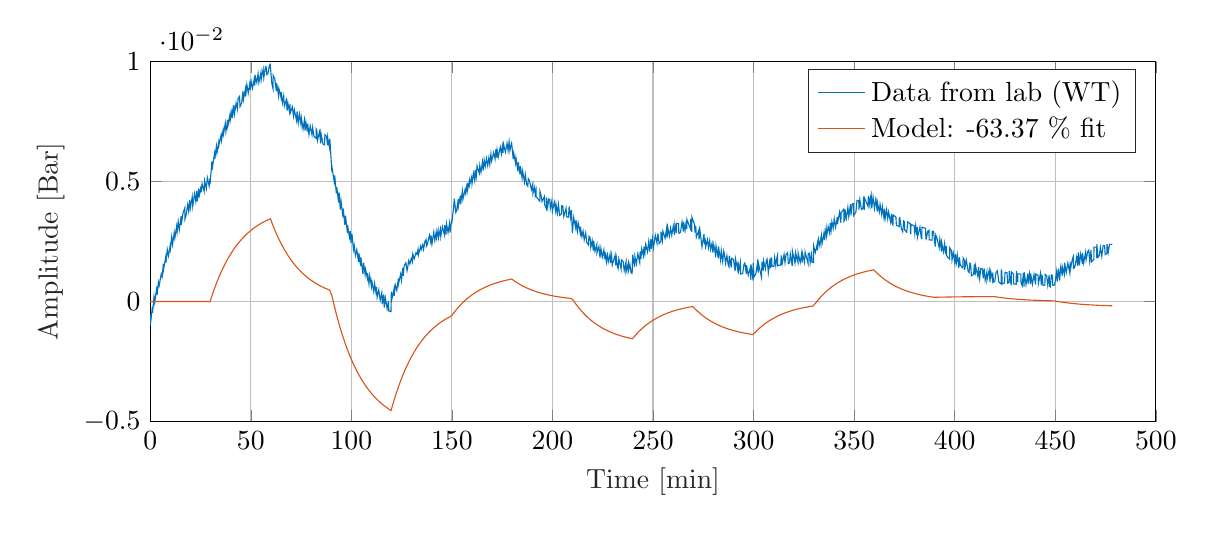
\begin{tikzpicture}

\begin{axis}[%
width=5.028in,
height=1.8in,
at={(1.011in,0.642in)},
scale only axis,
xmin=0,
xmax=500,
xlabel style={font=\color{white!15!black}},
xlabel={Time [min]},
ymin=-0.005,
ymax=0.01,
ylabel style={font=\color{white!15!black}},
ylabel={Amplitude [Bar]},
axis background/.style={fill=white},
%title style={font=\bfseries},
%title={Node WT},
xmajorgrids,
ymajorgrids,
legend style={legend cell align=left, align=left, draw=white!15!black}
]
\addplot [color=mycolor1]
  table[row sep=crcr]{%
0.000833333333333333	-0.000536486839485997\\
0.0508333333333333	-0.000992361717296275\\
1.07083333333333	-0.000214590456297223\\
1.15416666666667	-0.000472107562845242\\
1.86083333333333	0.000207354802741866\\
2.23	-4.84223233562925e-05\\
3.3075	0.000626690091107954\\
3.38583333333333	0.00026912410870214\\
4.09666666666667	0.000805908077422438\\
4.44416666666667	0.000669319612141839\\
5.46916666666667	0.00114433427489903\\
5.94	0.00103123554567336\\
6.4975	0.00157758940687817\\
6.65083333333333	0.00135139194838989\\
7.67916666666667	0.00184728637653113\\
7.8475	0.00162804883988631\\
8.4725	0.0021700527499505\\
9.06583333333333	0.00190383574114041\\
9.86583333333333	0.00231708109796219\\
10.0333333333333	0.00219441247628542\\
10.6625	0.00268682694352837\\
11.0708333333333	0.00237276047235473\\
11.9325	0.00287561482232949\\
12.2391666666667	0.00264245744206168\\
13.1041666666667	0.00312878197772765\\
13.3541666666667	0.00290519448994932\\
13.9108333333333	0.00333583965122845\\
14.45	0.00299306350267163\\
15.3741666666667	0.00356551707060934\\
15.4558333333333	0.00319925118595282\\
16.3025	0.00368905568249719\\
17.1833333333333	0.00390046330714998\\
17.2666666666667	0.00343501853685101\\
17.7641666666667	0.00356899703145931\\
18.6308333333333	0.00404227171378015\\
19.0908333333333	0.00377257474405045\\
19.6383333333333	0.00423018960235598\\
19.9341666666667	0.00388045353190596\\
20.8775	0.00436242811647393\\
21.1391666666667	0.00397441247625356\\
22.0441666666667	0.0044946666306203\\
22.67	0.00417973016928958\\
23.1425	0.00461211531109033\\
23.3208333333333	0.00417886017903019\\
24.1791666666667	0.00470868422599441\\
24.2483333333333	0.00433110846838648\\
25.3183333333333	0.00482178295526413\\
25.3691666666667	0.00455295597579951\\
25.79	0.0049087819777299\\
26.8133333333333	0.00458514561404404\\
27.0483333333333	0.0050358005505473\\
27.8891666666667	0.00470172430424899\\
28.3883333333333	0.00516716907457639\\
29.2941666666667	0.00481656301394655\\
29.7325	0.0051523792407011\\
29.7625	0.00490095206570235\\
30.6466666666667	0.00583619155747787\\
30.9566666666667	0.00560738412834215\\
31.9533333333333	0.00616591785262703\\
32.1408333333333	0.00594842029645977\\
32.8883333333333	0.00647563437269132\\
33.1991666666667	0.00620158745181247\\
34.0508333333333	0.00664006252517314\\
34.1708333333333	0.00652087386437759\\
35.2375	0.00694281912341242\\
35.4483333333333	0.00672184160628152\\
36.2408333333333	0.00713334698266412\\
36.4483333333333	0.00697674874195404\\
37.3158333333333	0.00742740367857099\\
37.6408333333333	0.00707940758862836\\
38.46	0.00757269204601703\\
38.6225	0.00731604492973477\\
39.6466666666667	0.00780062948502976\\
39.7975	0.00756138217316223\\
40.6383333333333	0.0079667976179849\\
40.7991666666667	0.00765708109780693\\
41.6566666666667	0.00818690514487348\\
41.8908333333333	0.00782411922099303\\
42.715	0.00827129419660654\\
43.3516666666667	0.00802073701192969\\
43.67	0.00845747210482846\\
44.3908333333333	0.0085496910686516\\
44.6391666666667	0.00811904590741509\\
45.4466666666667	0.00827303417712531\\
46.12	0.00876283867381748\\
46.3391666666667	0.0084157125740376\\
47.34	0.00886201755934056\\
47.4641666666667	0.00854534111753087\\
48.0433333333333	0.00904210553595707\\
48.7341666666667	0.00868540954363657\\
49.5266666666667	0.00909604492984502\\
49.745	0.00882373798954179\\
50.2425	0.00916390416738298\\
50.8483333333333	0.00889420719768171\\
51.74	0.00929005275006607\\
51.8875	0.00899686604425372\\
52.3775	0.00934312215351842\\
52.9958333333333	0.00912388461709955\\
53.6241666666667	0.0094927604723694\\
54.0066666666667	0.00912823456810659\\
55.0375	0.00955452977834743\\
55.165	0.0092430732779349\\
56.1508333333333	0.00968241834136736\\
56.4716666666667	0.00932572234918329\\
57.2933333333333	0.00978159722704962\\
57.5741666666667	0.0097902971291433\\
57.9783333333333	0.00945274092208596\\
58.5308333333333	0.00950929028662136\\
59.2725	0.0098451065133759\\
59.645	0.009886866044144\\
60.4433333333333	0.00909865490045834\\
61.0316666666667	0.00887158745175616\\
61.1091666666667	0.00942490123472912\\
61.9116666666667	0.00928483280862343\\
62.6825	0.0087697985954492\\
62.86	0.00909604492984502\\
63.8058333333333	0.00856796086343369\\
63.9925	0.00886897748114283\\
64.995	0.00851315147931477\\
65.1666666666667	0.00872716907451836\\
65.7458333333333	0.00828695402080944\\
66.3466666666667	0.00856883085373288\\
66.6825	0.00814340563367753\\
67.6433333333333	0.00840266272052763\\
68.0608333333333	0.00795896770581524\\
68.4358333333333	0.00827390416728808\\
69.1133333333333	0.00795374776472503\\
69.5491666666667	0.00822692469517965\\
69.5725	0.00784586897667626\\
70.65	0.00811034600502585\\
71.2266666666667	0.00772494033525394\\
71.6541666666667	0.00798419742237687\\
72.7375	0.00754050240778954\\
73.01	0.00791720817486526\\
73.6141666666667	0.00744828344392094\\
74.1575	0.00781106936782412\\
74.9383333333333	0.00738390416730685\\
75.115	0.00766665099071136\\
76.005	0.00719424629820654\\
76.65	0.00756399214379828\\
76.955	0.00711942713888906\\
77.415	0.00746307327787012\\
78.0891666666667	0.00708201755936673\\
78.2833333333333	0.00740913388382299\\
78.9216666666667	0.00695325900600215\\
79.5525	0.0073247448319876\\
80.4225	0.00694977904523743\\
80.7716666666667	0.00725253564354493\\
81.3908333333333	0.00688365978818413\\
82.4541666666667	0.00680275069711346\\
82.5333333333333	0.00718293642545408\\
82.8233333333333	0.00713421697295193\\
83.1758333333333	0.0067183616453463\\
84.1275	0.00706809771546664\\
84.8033333333333	0.00658960309225452\\
84.8933333333333	0.00701241834125317\\
85.9116666666667	0.0065565434635005\\
86.6733333333333	0.00652870377638241\\
86.8425	0.00695325900604761\\
87.67	0.00687843984666191\\
88.1383333333333	0.00650869400120659\\
88.2233333333333	0.0068323303650573\\
89.1141666666667	0.00642778491038602\\
89.2983333333333	0.0067879608633007\\
90.3308333333333	0.00538205665992568\\
90.4525	0.0055621446368264\\
91.4575	0.00500187093206254\\
91.7041666666667	0.00525851804817425\\
92.54	0.0045085864743783\\
92.7266666666667	0.00477045353203497\\
93.6683333333333	0.0041240507948601\\
93.8883333333333	0.00454947601482449\\
94.51	0.00382999409893049\\
94.8683333333333	0.00419104004230351\\
95.8275	0.00350983769623102\\
95.955	0.0038752335908271\\
96.76	0.00318794131306963\\
97.1091666666667	0.00357421697282238\\
98.0425	0.00285995499820051\\
98.1075	0.00319490123468999\\
99.0458333333333	0.00267899703131892\\
99.4766666666667	0.00293564414743062\\
99.8283333333333	0.0024319198074068\\
100.315833333333	0.00281993544775791\\
101.033333333333	0.00216657278884899\\
101.403333333333	0.00234405079478396\\
102.028333333333	0.00192471550636814\\
102.680833333333	0.00216396281815609\\
103.588333333333	0.001644578654134\\
103.755	0.00201258451930929\\
104.6	0.00147493056018679\\
104.76	0.00184032645473739\\
105.77	0.00114259429432199\\
106.074166666667	0.00161673896674305\\
106.840833333333	0.00112432449958537\\
107.080833333333	0.00133486213409245\\
107.939166666667	0.000972076210166539\\
108.080833333333	0.00118087386405254\\
108.774166666667	0.000732828898560495\\
109.131666666667	0.00108604492980934\\
110.001666666667	0.000624080120462653\\
110.216666666667	0.000841577676476427\\
111.150833333333	0.000406582564357938\\
111.563333333333	0.000743268781309356\\
112.415	0.000279563991478007\\
112.455833333333	0.000609290286672642\\
112.814166666667	0.000178645125436139\\
113.62	0.000489231635367599\\
114.365	4.81465916778168e-05\\
115.125833333333	0.000368302994468231\\
115.4075	-0.000117151550909925\\
116.065	0.00029870377637739\\
116.373333333333	-0.000248520074990169\\
116.908333333333	0.000155155389177292\\
117.788333333333	-0.000298109517950673\\
118.435	2.98767968957142e-05\\
118.604166666667	-0.000388588501198189\\
119.695833333333	-0.000419908149149217\\
119.880833333333	0.000413542486114735\\
120.1675	0.000105565946603325\\
121.139166666667	0.000501411498828513\\
121.283333333333	0.000227364577756392\\
121.854166666667	0.000693679338462552\\
122.6025	0.000460521958063995\\
123.380833333333	0.000961636327417678\\
123.4625	0.000743268781309356\\
124.504166666667	0.00114694424531767\\
124.9125	0.000882467217309155\\
125.5225	0.00139924141050191\\
125.796666666667	0.00107560504699226\\
126.219166666667	0.00148015050157259\\
127.1175	0.00161847894747784\\
127.699166666667	0.00128179273038999\\
128.011666666667	0.00140707132280798\\
128.468333333333	0.00170286799931323\\
129.098333333333	0.00156279957299152\\
129.788333333333	0.00180204688484768\\
130.3225	0.00165849849767032\\
130.539166666667	0.00198561482230847\\
131.248333333333	0.00178203710974006\\
132.12	0.0020352042650416\\
132.608333333333	0.00196995499810558\\
133.1375	0.00217962264219981\\
133.405833333333	0.0019525551938273\\
134.408333333333	0.00230316125424683\\
134.744166666667	0.00216309282819797\\
135.503333333333	0.00237363046250043\\
135.891666666667	0.00217788266171513\\
136.6675	0.00253457865395607\\
137.1925	0.00258851804782129\\
137.335833333333	0.00230490123493614\\
137.84	0.00238494033595775\\
138.808333333333	0.00276425607384002\\
139.506666666667	0.00246062948502872\\
139.593333333333	0.00275642616232975\\
140.186666666667	0.00245105959292008\\
140.965	0.00289475460775751\\
141.4925	0.00255110846823076\\
142.175833333333	0.00290171452942335\\
142.408333333333	0.00265115734435999\\
143.1275	0.00297740367904002\\
143.38	0.00266420719816556\\
144.2375	0.0030243831514213\\
144.466666666667	0.00270596672902461\\
145.256666666667	0.00311747210483876\\
146.374166666667	0.0027546861811857\\
146.4575	0.00318794131306963\\
147.056666666667	0.00280166565411268\\
147.330833333333	0.00322970084361035\\
148.071666666667	0.0028773548032746\\
148.791666666667	0.00325145059977107\\
149.050833333333	0.00287213486170688\\
149.860833333333	0.00340369888939453\\
149.893333333333	0.00325058060979021\\
150.83	0.0039135131604667\\
151.1775	0.00428847894744426\\
151.945	0.00371689536958687\\
152.315833333333	0.00378997454862433\\
153.1525	0.00426411922152287\\
153.238333333333	0.0039657125741883\\
154.2325	0.00442506741263746\\
154.315833333333	0.00405358158662925\\
155.198333333333	0.00460341540850781\\
155.4825	0.00426324923136011\\
156.505	0.00465735480250945\\
156.8	0.00451641638672985\\
157.609166666667	0.00493749165510739\\
157.6975	0.00461820524259342\\
158.700833333333	0.00503754053132756\\
158.765	0.00485658256478703\\
159.806666666667	0.00519326878155656\\
159.993333333333	0.00490617200701994\\
160.8075	0.0053516070025012\\
161.3525	0.00505581032551848\\
161.619166666667	0.00547688559498742\\
162.095833333333	0.00520022870363167\\
162.490833333333	0.00565175362988841\\
163.600833333333	0.00534203710998331\\
163.851666666667	0.00566654346388308\\
164.450833333333	0.00538466663091416\\
165.16	0.00582575167444478\\
165.6125	0.00545426584843657\\
166.054166666667	0.00589361091196002\\
166.581666666667	0.00563435382495077\\
167.184166666667	0.0059571201987524\\
167.7825	0.00566654346338287\\
168.3725	0.00599713974860382\\
168.805	0.00571700289646064\\
169.3875	0.00614677806805734\\
169.758333333333	0.00585620133305161\\
170.738333333333	0.00620854737334188\\
171.451666666667	0.00594059038461413\\
171.8825	0.00635209576097399\\
172.335833333333	0.00599365978804374\\
172.491666666667	0.00630511628886556\\
173.075833333333	0.00603280934827811\\
174.026666666667	0.00644257474422151\\
174.6175	0.00615721795001041\\
175.04	0.0064643245002458\\
175.360833333333	0.00618331765789439\\
175.693333333333	0.00655741345389065\\
176.583333333333	0.00622681716853325\\
177.395	0.00659917298493158\\
177.9325	0.00628684649394702\\
178.433333333333	0.00665920231057275\\
178.843333333333	0.0062868464943563\\
179.63	0.00661570279925176\\
179.706666666667	0.00660178295482867\\
180.4625	0.00593711042378121\\
180.76	0.00617635773527357\\
181.635833333333	0.00576311237872464\\
181.86	0.00597625998365177\\
182.786666666667	0.0054264261610911\\
183.0075	0.0058040019189662\\
183.839166666667	0.00530549752032815\\
184.069166666667	0.00563696379589378\\
184.88	0.00514367933859607\\
185.18	0.00543599605383636\\
186.074166666667	0.0049818611570004\\
186.4975	0.00529157767649625\\
187.1575	0.0048765923396218\\
187.725833333333	0.00480873310197015\\
188.004166666667	0.00511931961240183\\
188.5525	0.00504363046255779\\
189.555	0.00466518471465636\\
190.189166666667	0.00488964219260883\\
190.2725	0.00450249654303438\\
191.14	0.00476871355175494\\
191.398333333333	0.00445029712963109\\
191.813333333333	0.0046173352532492\\
191.844166666667	0.00437547797045003\\
193.7	0.00418147015033131\\
193.783333333333	0.00458949556563087\\
194.255	0.00444594717845352\\
194.815833333333	0.00417364023841177\\
195.985833333333	0.00437982792121833\\
196.06	0.00404836164551629\\
196.933333333333	0.00386914365898296\\
197.0175	0.00434067836112038\\
197.603333333333	0.00392917298521528\\
198.156666666667	0.00427629908507474\\
198.6375	0.00425802929006526\\
198.944166666667	0.00387784356206571\\
199.669166666667	0.00419191003314839\\
199.9775	0.0037664848125019\\
200.915	0.00414928051180827\\
201.564166666667	0.0037725747443233\\
201.768333333333	0.004033571811749\\
202.4675	0.00367687581978092\\
202.929166666667	0.00405184160612183\\
203.621666666667	0.00359161677714613\\
204.505	0.00365251609299552\\
204.585833333333	0.00399094229022698\\
205.1475	0.0039865923394132\\
205.626666666667	0.00354985724683278\\
206.756666666667	0.00389002342470807\\
207.026666666667	0.0035254975203657\\
207.9675	0.00351505763754861\\
208.286666666667	0.00395875265261342\\
209.04	0.00348634796044965\\
209.41	0.00380650436303544\\
209.411666666667	0.003812594294584\\
209.891666666667	0.00285473505736039\\
210.5625	0.00350287777404222\\
211.525833333333	0.00307745255462354\\
211.723333333333	0.00338542909456695\\
212.393333333333	0.00294173407995689\\
212.790833333333	0.00327059038417023\\
213.818333333333	0.00284951511602007\\
213.905833333333	0.00311660211476696\\
214.634166666667	0.00270422674806245\\
215.219166666667	0.00293738412837005\\
215.784166666667	0.00256589830254374\\
216.515833333333	0.00286343495948817\\
217.0375	0.00246323945660837\\
217.864166666667	0.00236145059951699\\
218.144166666667	0.0027146666312888\\
218.6975	0.00267116712001329\\
219.034166666667	0.00225009185086268\\
219.7325	0.00253892860536102\\
220.304166666667	0.0021256832485847\\
220.466666666667	0.00253805861560753\\
221.120833333333	0.00209610358141393\\
222.034166666667	0.00237015050169025\\
222.084166666667	0.00201867445101701\\
223.091666666667	0.0022883714202067\\
223.623333333333	0.0018377164846584\\
224.093333333333	0.0022266021144674\\
224.74	0.00184206643579049\\
225.549166666667	0.00215091296530549\\
225.881666666667	0.00178029712923265\\
226.07	0.00207783378617708\\
226.785833333333	0.00165066858606909\\
227.296666666667	0.00204651413822607\\
227.7325	0.0016463186351189\\
228.655833333333	0.00197256496916229\\
228.861666666667	0.00160542909446808\\
229.399166666667	0.00192471550730038\\
229.7125	0.00151495011044749\\
231.155	0.00193602537959808\\
231.414166666667	0.00150712019839151\\
231.775833333333	0.00181248676798308\\
232.34	0.00143404101949049\\
232.639166666667	0.00137227171379667\\
232.999166666667	0.00178029712941456\\
234.129166666667	0.00135574189988578\\
234.308333333333	0.00173940758867279\\
235.156666666667	0.00166371843987466\\
235.661666666667	0.00129484258380902\\
236.54	0.00165414854672012\\
236.575	0.00123481325857715\\
237.670833333333	0.0016002091528549\\
237.693333333333	0.00126178295512322\\
238.505	0.00155931961184028\\
239.070833333333	0.00119044375650222\\
239.6075	0.00117391394240944\\
239.890833333333	0.00195429517460756\\
240.770833333333	0.00144361091214482\\
240.981666666667	0.00188034600531641\\
241.724166666667	0.00157149947530119\\
242.4275	0.00199170475401619\\
243.393333333333	0.00162021892778061\\
243.575833333333	0.00209262362021721\\
243.964166666667	0.00176898725625282\\
244.370833333333	0.00219876242762215\\
245.205	0.00190557572271931\\
245.478333333333	0.00228489146019233\\
245.949166666667	0.00199866467600035\\
246.354166666667	0.0023849403364125\\
247.235	0.00207261384506413\\
247.829166666667	0.00248933916312812\\
248.329166666667	0.00208044375707463\\
248.8375	0.00259895793068385\\
249.189166666667	0.00220050240808409\\
249.7075	0.00261461775579623\\
250.246666666667	0.00224835187026433\\
251.099166666667	0.002765996054211\\
251.9675	0.00242582987633572\\
252.328333333333	0.00280775558525197\\
252.44	0.00281210553670239\\
253.056666666667	0.00240843007194375\\
253.8975	0.0025180488399997\\
253.983333333333	0.00291563437293693\\
254.624166666667	0.00255023847834085\\
254.914166666667	0.00293651413852562\\
255.990833333333	0.00264158745266062\\
256.754166666667	0.00305570279941779\\
256.984166666667	0.0026502873544246\\
257.270833333333	0.0031157321244223\\
258.0975	0.00271988657240176\\
258.724166666667	0.00306875265308694\\
259.311666666667	0.00276686604410091\\
260.065833333333	0.00315053173316077\\
260.6775	0.00278165587832295\\
260.901666666667	0.00321230103949123\\
261.615833333333	0.0028521250865538\\
261.699166666667	0.0032523205899793\\
262.6825	0.00324884062919185\\
262.825	0.00284429517467974\\
263.676666666667	0.00289301462684083\\
264.419166666667	0.00332017982713072\\
265.101666666667	0.00291911433363343\\
265.186666666667	0.00331930983696797\\
265.890833333333	0.00294956399196739\\
266.551666666667	0.00336280934869823\\
266.7825	0.00302699312186409\\
266.865	0.00341587875230974\\
268.590833333333	0.00303569302376448\\
268.773333333333	0.00344545841975336\\
269.238333333333	0.00289997454923427\\
269.3225	0.00351418764734039\\
270.565	0.00322883085349307\\
270.881666666667	0.00287735480300175\\
271.269166666667	0.00315053173366099\\
271.513333333333	0.00268073701262214\\
272.8425	0.00299828344431038\\
272.875833333333	0.00259547797007829\\
273.335833333333	0.00296000387442068\\
274.323333333333	0.00228402146984767\\
275.316666666667	0.00281123554599393\\
275.539166666667	0.00238494033577584\\
275.8475	0.00265376731539395\\
276.171666666667	0.00227793153734414\\
277.071666666667	0.00258764805674903\\
277.536666666667	0.00224139194777993\\
278.160833333333	0.00254066858495892\\
278.6025	0.00216570279816328\\
279.3575	0.00243539976671631\\
279.738333333333	0.00203607425481782\\
280.2075	0.00237102049085255\\
281.035833333333	0.00195429517324332\\
281.131666666667	0.00184293642504375\\
281.3275	0.00231447112599885\\
282.463333333333	0.00179769693339725\\
282.5475	0.00229533134150874\\
283.586666666667	0.00171765783314871\\
283.935	0.00211872332555461\\
284.645	0.00166284844871147\\
285.168333333333	0.00209871355162936\\
285.479166666667	0.00199083476344417\\
286.078333333333	0.00159150925018142\\
286.728333333333	0.00191253564133835\\
287.343333333333	0.00153669986619892\\
287.755833333333	0.00145057083344685\\
287.929166666667	0.00191340563295629\\
288.8725	0.00142099116554849\\
289.056666666667	0.00180291687473759\\
289.9725	0.00175854737252625\\
290.835833333333	0.00126526291604709\\
290.9875	0.0017776871578349\\
292.059166666667	0.00133486213416066\\
292.293333333333	0.00166458842949173\\
292.654166666667	0.00127396281831128\\
293.415833333333	0.00162891882945364\\
293.560833333333	0.00114694424554504\\
294.574166666667	0.00117130397237591\\
295.185833333333	0.00154539976864503\\
295.633333333333	0.00160281912347958\\
296.4	0.00115564414871873\\
296.49	0.00151234013973184\\
297.338333333333	0.00109822479324752\\
298.370833333333	0.00142012117556764\\
298.639166666667	0.000892907099921597\\
298.723333333333	0.00154191980699356\\
299.735	0.000878987257226557\\
299.818333333333	0.00160716907402052\\
300.2225	0.00102775558533498\\
301.149166666667	0.0011573841273162\\
301.861666666667	0.00158628930829539\\
302.311666666667	0.00121045353261028\\
302.393333333333	0.00160803906418326\\
303.900833333333	0.00101470573289365\\
304.184166666667	0.00165153857586806\\
304.766666666667	0.00129310260289234\\
304.9575	0.00169938803782092\\
305.860833333333	0.00135835187073784\\
306.335	0.00171765783287586\\
306.685	0.00177681716739929\\
307.318333333333	0.0012121935118444\\
308.164166666667	0.00179334698231064\\
308.2475	0.00138619155803785\\
308.95	0.00183597650328697\\
309.165833333333	0.00146362068779812\\
310.108333333333	0.00147145059880817\\
310.474166666667	0.00184119644417255\\
311.023333333333	0.00149929028583533\\
311.6425	0.00185511628759517\\
311.924166666667	0.00194907523108444\\
311.993333333333	0.00149059038329828\\
313.476666666667	0.00152712997440861\\
313.768333333333	0.00192645548603426\\
314.201666666667	0.00156366956369997\\
315.143333333333	0.00196299507532562\\
315.601666666667	0.00162717884885527\\
316.098333333333	0.00196038510520115\\
316.8975	0.00203520426520075\\
317.2575	0.00158628930820445\\
317.854166666667	0.00161151902501619\\
318.255833333333	0.00198648481226658\\
319.21	0.0014862404323026\\
319.298333333333	0.00210306350171553\\
320.500833333333	0.00161412899568635\\
320.69	0.00200040465523448\\
320.839166666667	0.00163413877115776\\
320.9175	0.00203172430291264\\
322.065833333333	0.0016323987901956\\
322.149166666667	0.00202824434244352\\
323.178333333333	0.0016323987898318\\
323.925833333333	0.00202998432267808\\
324.149166666667	0.00160890905507362\\
324.2325	0.00203694424443487\\
325.323333333333	0.0016332687808131\\
325.594166666667	0.00206739390258694\\
327.071666666667	0.00159498921119625\\
327.155	0.00198735480115605\\
327.753333333333	0.00201780445994476\\
328.114166666667	0.00161064903530818\\
328.758333333333	0.00196473505583303\\
329.06	0.00163413877170346\\
329.755	0.00162717884949191\\
329.841666666667	0.00232839097042191\\
330.665	0.00204042420526779\\
331.738333333333	0.00244322967936345\\
331.764166666667	0.00213786311013568\\
332.288333333333	0.00259199800801756\\
332.9175	0.00232143104730088\\
333.6775	0.00275903613190852\\
333.9975	0.00239712019846369\\
335.015833333333	0.00287735480150107\\
335.255	0.00256241834084679\\
336.065	0.00306614268118896\\
336.334166666667	0.00272945646373732\\
337.068333333333	0.0031218220560618\\
337.800833333333	0.00284603515455049\\
338.108333333333	0.00326972039355272\\
338.54	0.00297392371793424\\
338.9075	0.00332626975831549\\
339.575833333333	0.00305570279878115\\
340.0975	0.00345241834173753\\
340.745	0.0031018122809542\\
341.628333333333	0.00351853759838154\\
341.668333333333	0.00322361091210727\\
342.7225	0.00372472528223401\\
343.404166666667	0.00327842029518027\\
343.478333333333	0.00369775558482392\\
344.9075	0.00385522381501463\\
344.936666666667	0.00334714952322206\\
345.384166666667	0.00341065881128774\\
345.468333333333	0.00383434405047187\\
346.135	0.00347764805718502\\
346.8675	0.00392569302374572\\
347.3175	0.00354463730471938\\
348.179166666667	0.00405793153785229\\
348.426666666667	0.00359596672832371\\
349.1075	0.00407881130266791\\
349.726666666667	0.00408403124555438\\
349.755	0.00358552684637065\\
350.864166666667	0.00372646526310522\\
351.400833333333	0.00421452977860785\\
352.269166666667	0.00420930983772226\\
352.418333333333	0.00383434404983522\\
352.825833333333	0.00424323945752579\\
353.6225	0.00383173408025644\\
354.305	0.00387436360050518\\
354.7875	0.00436938803812841\\
355.030833333333	0.00381607425496217\\
355.1125	0.00431283867336564\\
356.963333333333	0.00396136262323811\\
357.045833333333	0.00438939781460025\\
357.815	0.00399094229086362\\
357.995	0.00430152880052223\\
358.451666666667	0.00446247699209155\\
358.741666666667	0.00388915343381772\\
359.403333333333	0.00435894815517489\\
360.095833333333	0.00387523359048604\\
360.716666666667	0.00424671941672163\\
361.505	0.00375343495860538\\
361.5725	0.00413623066004906\\
362.488333333333	0.00373516516364138\\
362.871666666667	0.00404836164442489\\
363.680833333333	0.00363424629866817\\
364.046666666667	0.00395179273081116\\
364.771666666667	0.00352114756841505\\
365.053333333333	0.00385696379606774\\
365.450833333333	0.0034759080768595\\
366.105833333333	0.00382912410813109\\
366.700833333333	0.0034411084688941\\
367.151666666667	0.00373429517438811\\
368.115	0.00331582987581673\\
368.621666666667	0.00364642616312953\\
368.876666666667	0.00324797063848341\\
369.27	0.00319142127372064\\
369.4375	0.0036029266504443\\
370.769166666667	0.00352375754008566\\
370.985	0.00317576144869922\\
372.423333333333	0.00312791198711014\\
372.441666666667	0.00346720817532291\\
372.683333333333	0.003493307881206\\
373.478333333333	0.00303830299334326\\
374.13	0.00291041442995951\\
374.654166666667	0.00335671941683134\\
375.045	0.0033193098361949\\
375.143333333333	0.00298001364889164\\
376.146666666667	0.00288692469529227\\
376.610833333333	0.00331756985668794\\
377.888333333333	0.00324623065715744\\
378.021666666667	0.00287039488092664\\
378.129166666667	0.00280775558429699\\
378.280833333333	0.00321752097996754\\
379.829166666667	0.003156621664391\\
380.155	0.0028442951733155\\
380.603333333333	0.00317315147848379\\
381.168333333333	0.00276686604310047\\
381.405	0.0031018122811361\\
381.488333333333	0.00268508696225357\\
382.704166666667	0.00310355226073401\\
383.408333333333	0.00262853759767272\\
383.6025	0.00262157767591592\\
383.683333333333	0.003100072300083\\
385.525833333333	0.00305222283658399\\
385.653333333333	0.00261983769549946\\
385.7975	0.00260156790044451\\
386.628333333333	0.00294086408829347\\
387.2225	0.0029713137461727\\
387.245833333333	0.00257111824292909\\
388.753333333333	0.00255632840861612\\
388.846666666667	0.00292172430425812\\
389.454166666667	0.00293042420597661\\
390.058333333333	0.00246236946439925\\
390.344166666667	0.00228750142931634\\
390.585833333333	0.00277469595411052\\
391.265833333333	0.00261200778385277\\
392.271666666667	0.00223965196654494\\
392.604166666667	0.0025980879401573\\
393.464166666667	0.00208392371695258\\
393.544166666667	0.00245714952433222\\
394.4	0.00207783378581329\\
394.961666666667	0.00241538999315484\\
395.445	0.00197430494844188\\
395.774166666667	0.00230403124286344\\
395.988333333333	0.00190818569152501\\
397.4675	0.00176637728453674\\
397.545	0.00223791198585563\\
398.365	0.00212568324803901\\
398.661666666667	0.00173940758839994\\
399.241666666667	0.00203259429425774\\
400.021666666667	0.00160716907438431\\
400.294166666667	0.00197343495837007\\
400.805833333333	0.00162108891880738\\
401.275	0.00194820524237688\\
402.045	0.00140011140055098\\
402.3325	0.00184467640555117\\
402.779166666667	0.00151495011040201\\
404.080833333333	0.0013975014307903\\
404.159166666667	0.00181944668919418\\
404.886666666667	0.00171765783269397\\
404.919166666667	0.00132181228090079\\
405.76	0.00172287777476189\\
406.674166666667	0.00126178295557797\\
407.135833333333	0.00121306350200716\\
407.583333333333	0.00159933916237381\\
407.891666666667	0.00157845939619396\\
408.323333333333	0.00107212508572734\\
409.380833333333	0.00114172430438661\\
409.74	0.0015497497203683\\
410.174166666667	0.00109300485127055\\
410.255833333333	0.00151930006176147\\
411.514166666667	0.00104776536089733\\
411.856666666667	0.00143926096042155\\
412.4075	0.000963376307379388\\
412.975	0.00138706154747301\\
413.7275	0.0013600918509724\\
414.178333333333	0.000969466240519565\\
414.638333333333	0.0013766216645195\\
415.12	0.000898127042353314\\
416.009166666667	0.00123655323931192\\
416.031666666667	0.000892907100285389\\
417.148333333333	0.00130615245651601\\
417.5325	0.000813737990108657\\
417.906666666667	0.00125482303282073\\
418.781666666667	0.000898127041443819\\
418.910833333333	0.00120088363991049\\
419.2925	0.000810258028275293\\
419.920833333333	0.000842447666570975\\
420.500833333333	0.00120523359145185\\
421.184166666667	0.00128092274097756\\
421.975833333333	0.000805038087116863\\
423.079166666667	0.000730218927844847\\
423.163333333333	0.00130615245769836\\
423.4575	0.00127048285738741\\
423.511666666667	0.000734568878203876\\
424.706666666667	0.000770238478514818\\
425.04	0.00122263339470695\\
425.976666666667	0.00120523359054235\\
426.383333333333	0.000762408566322426\\
427.003333333333	0.000799818146413181\\
427.086666666667	0.00128092273979523\\
428.054166666667	0.000677149524096907\\
428.233333333333	0.00123220328749771\\
429.253333333333	0.00115042420601416\\
429.2825	0.000734568879386222\\
430.565833333333	0.000720649036782137\\
430.65	0.00127483280920164\\
431.350833333333	0.000810258029002892\\
431.44	0.00115129419672261\\
432.860833333333	0.00115129419745021\\
432.979166666667	0.000792858224565443\\
433.5375	0.000658009738606358\\
434.141666666667	0.00119305372671764\\
434.469166666667	0.000626690091110091\\
434.551666666667	0.00121828344452983\\
435.449166666667	0.000704119222234609\\
436.378333333333	0.00117391394231849\\
436.495	0.000732828899333557\\
437.1925	0.00115303417741192\\
437.654166666667	0.000722389015561514\\
437.729166666667	0.0011686940016148\\
438.663333333333	0.000723259007543262\\
439.4075	0.00113041443217984\\
440.228333333333	0.000704989211942605\\
440.310833333333	0.00114955421539666\\
441.473333333333	0.00108952489116522\\
441.593333333333	0.000740658811344053\\
442.635833333333	0.00117652391389815\\
443.065833333333	0.000683239456509485\\
443.431666666667	0.00112084454057143\\
443.889166666667	0.000672799573919788\\
444.8	0.000685849426633953\\
444.981666666667	0.00113215441214155\\
445.685	0.0010860449301504\\
446.265	0.000676279533661311\\
446.933333333333	0.00110170475380759\\
447.2425	0.000629300061598351\\
447.55	0.000609290286399791\\
448.026666666667	0.00110953466618188\\
448.576666666667	0.00107995499828352\\
448.758333333333	0.000679759495221824\\
449.6825	0.000686719417615264\\
450.643333333333	0.00124351316097776\\
450.9575	0.000830267804019555\\
451.579166666667	0.00136879175250901\\
452.1425	0.000876377285192159\\
452.709166666667	0.00144100094092896\\
453.4975	0.00107821501759421\\
453.575833333333	0.00143143104877484\\
454.539166666667	0.00112171452936995\\
454.62	0.00162108891762504\\
455.485833333333	0.00121480348251456\\
456.2475	0.00159933916146432\\
457.2025	0.00118870377635862\\
457.3875	0.00165936848769664\\
457.511666666667	0.00132181228080984\\
458.450833333333	0.0017515874508604\\
458.930833333333	0.00187251609276022\\
459.0675	0.00138271159620448\\
459.643333333333	0.00142012117520383\\
460.675833333333	0.0018690361317454\\
461.1	0.00149233036398759\\
461.5725	0.00204564414724477\\
461.985	0.00150886017862607\\
462.648333333333	0.001986484811539\\
463.486666666667	0.00156714952453289\\
463.569166666667	0.00202128442050484\\
464.115	0.00161064903539913\\
465.079166666667	0.00205695402054293\\
465.31	0.00174027757828985\\
466.140833333333	0.00208392371740733\\
466.655	0.00214134307124145\\
467.113333333333	0.00168024825196657\\
467.778333333333	0.00214047308171533\\
468.005	0.00165762850737114\\
469.170833333333	0.00175506741151142\\
469.253333333333	0.00226401169364866\\
470.563333333333	0.00227184160529535\\
470.586666666667	0.00182118666897399\\
470.67	0.00239538021768343\\
471.190833333333	0.00184119644517299\\
471.875833333333	0.00191253564261164\\
472.42	0.0022535718107861\\
473.109166666667	0.00188991589719766\\
473.813333333333	0.00233013095083838\\
474.513333333333	0.00233274092069\\
474.81	0.00195429517433471\\
475.64	0.00199083476271657\\
475.723333333333	0.00239538021795628\\
476.329166666667	0.00204564414597147\\
476.949166666667	0.00238581032543837\\
478.334166666667	0.00238320035404062\\
};
\addlegendentry{Data from lab (WT)}

\addplot [color=mycolor2]
  table[row sep=crcr]{%
0.000833333333333333	0\\
0.000833333333333333	0\\
1.10333333333333	-5.06498171062578e-16\\
1.10333333333333	-5.06498171062578e-16\\
2.20583333333333	-9.76845476540721e-16\\
2.20583333333333	-9.76845476540721e-16\\
3.3075	-1.41330407548488e-15\\
3.3075	-1.41330407548488e-15\\
4.41	-1.81892889974846e-15\\
4.41	-1.81892889974846e-15\\
5.51166666666667	-2.19532829745552e-15\\
5.51166666666667	-2.19532829745552e-15\\
6.61416666666667	-2.54513682435173e-15\\
6.61416666666667	-2.54513682435173e-15\\
7.71666666666667	-2.86997807247266e-15\\
7.71666666666667	-2.86997807247266e-15\\
8.81833333333333	-3.17141438215868e-15\\
8.81833333333333	-3.17141438215868e-15\\
9.92083333333333	-3.45155561534515e-15\\
9.92083333333333	-3.45155561534515e-15\\
11.0225	-3.71151256358124e-15\\
11.0225	-3.71151256358124e-15\\
12.125	-3.95310475972428e-15\\
12.125	-3.95310475972428e-15\\
13.2266666666667	-4.17729014404833e-15\\
13.2266666666667	-4.17729014404833e-15\\
14.3291666666667	-4.38563787127583e-15\\
14.3291666666667	-4.38563787127583e-15\\
15.4316666666667	-4.57911496103191e-15\\
15.4316666666667	-4.57911496103191e-15\\
16.5333333333333	-4.75865195112238e-15\\
16.5333333333333	-4.75865195112238e-15\\
17.6358333333333	-4.92550548598326e-15\\
17.6358333333333	-4.92550548598326e-15\\
18.7375	-5.08033715867713e-15\\
18.7375	-5.08033715867713e-15\\
19.84	-5.22423069217336e-15\\
19.84	-5.22423069217336e-15\\
20.9425	-5.35785395010874e-15\\
20.9425	-5.35785395010874e-15\\
22.0441666666667	-5.48184960027095e-15\\
22.0441666666667	-5.48184960027095e-15\\
23.1466666666667	-5.59708553313643e-15\\
23.1466666666667	-5.59708553313643e-15\\
24.2483333333333	-5.70401867216091e-15\\
24.2483333333333	-5.70401867216091e-15\\
25.3508333333333	-5.80339748112399e-15\\
25.3508333333333	-5.80339748112399e-15\\
26.4525	-5.89561600819868e-15\\
26.4525	-5.89561600819868e-15\\
27.555	-5.98131972426477e-15\\
27.555	-5.98131972426477e-15\\
28.6575	-6.06090641228102e-15\\
29.7525	-6.13432816906353e-15\\
29.7591666666667	1.78270662453254e-06\\
29.7591666666667	1.78270662453254e-06\\
30.8616666666667	0.00028588328038675\\
30.8616666666667	0.00028588328038675\\
31.9633333333333	0.000549514297167854\\
31.9633333333333	0.000549514297167854\\
33.0658333333333	0.000794521005962208\\
33.0658333333333	0.000794521005962208\\
34.1675	0.00102187488597133\\
34.1675	0.00102187488597133\\
35.27	0.00123316726936686\\
35.27	0.00123316726936686\\
36.3725	0.00142937884302303\\
36.3725	0.00142937884302303\\
37.4741666666667	0.00161145329638366\\
37.4741666666667	0.00161145329638366\\
38.5766666666667	0.00178066503450945\\
38.5766666666667	0.00178066503450945\\
39.6783333333333	0.00193768500100462\\
39.6783333333333	0.00193768500100462\\
40.7808333333333	0.00208361223549934\\
40.7808333333333	0.00208361223549934\\
41.8833333333333	0.00221912404079664\\
41.8833333333333	0.00221912404079664\\
42.985	0.00234487216774788\\
42.985	0.00234487216774788\\
44.0875	0.0024617367730494\\
44.0875	0.0024617367730494\\
45.1891666666667	0.00257018123802662\\
45.1891666666667	0.00257018123802662\\
46.2916666666667	0.00267096460477698\\
46.2916666666667	0.00267096460477698\\
47.3933333333333	0.0027644864907034\\
47.3933333333333	0.0027644864907034\\
48.4958333333333	0.00285140148936645\\
48.4958333333333	0.00285140148936645\\
49.5983333333333	0.00293211300573982\\
49.5983333333333	0.00293211300573982\\
50.7	0.0030070092259258\\
50.7	0.0030070092259258\\
51.8025	0.00307661437570275\\
51.8025	0.00307661437570275\\
52.9041666666667	0.00314120444733089\\
52.9041666666667	0.00314120444733089\\
54.0066666666667	0.00320123153012113\\
54.0066666666667	0.00320123153012113\\
55.1091666666667	0.00325697423218633\\
55.1091666666667	0.00325697423218633\\
56.2108333333333	0.00330870065085902\\
56.2108333333333	0.00330870065085902\\
57.3133333333333	0.00335677283808284\\
57.3133333333333	0.00335677283808284\\
58.415	0.00340138140549572\\
58.415	0.00340138140549572\\
59.5175	0.00344283858462169\\
59.7525	0.00345128528891706\\
60.6191666666667	0.00325612258718831\\
60.6191666666667	0.00325612258718831\\
61.7216666666667	0.00302371967499423\\
61.7216666666667	0.00302371967499423\\
62.8241666666667	0.00280790431813626\\
62.8241666666667	0.00280790431813626\\
63.9258333333333	0.0026076385417881\\
63.9258333333333	0.0026076385417881\\
65.0283333333333	0.00242152061322916\\
65.0283333333333	0.00242152061322916\\
66.13	0.00224881255390558\\
66.13	0.00224881255390558\\
67.2325	0.00208830551754178\\
67.2325	0.00208830551754178\\
68.3341666666667	0.00193936307565667\\
68.3341666666667	0.00193936307565667\\
69.4366666666667	0.00180094272614111\\
69.4366666666667	0.00180094272614111\\
70.5391666666667	0.00167240200844926\\
70.5391666666667	0.00167240200844926\\
71.6408333333333	0.00155312269952663\\
71.6408333333333	0.00155312269952663\\
72.7433333333333	0.00144226992027778\\
72.7433333333333	0.00144226992027778\\
73.845	0.00133940412694488\\
73.845	0.00133940412694488\\
74.9475	0.00124380532457432\\
74.9475	0.00124380532457432\\
76.05	0.00115502980341576\\
76.05	0.00115502980341576\\
77.1516666666667	0.00107265059312985\\
77.1516666666667	0.00107265059312985\\
78.2541666666667	0.000996091091779613\\
78.2541666666667	0.000996091091779613\\
79.3558333333333	0.000925047732317266\\
79.3558333333333	0.000925047732317266\\
80.4583333333333	0.000859023256532542\\
80.4583333333333	0.000859023256532542\\
81.56	0.000797755869941008\\
81.56	0.000797755869941008\\
82.6625	0.000740816739908063\\
82.6625	0.000740816739908063\\
83.765	0.00068794159066303\\
83.765	0.00068794159066303\\
84.8666666666667	0.000638876116513063\\
84.8666666666667	0.000638876116513063\\
85.9691666666667	0.000593276890429228\\
85.9691666666667	0.000593276890429228\\
87.0708333333333	0.000550963106343122\\
87.0708333333333	0.000550963106343122\\
88.1733333333333	0.000511638594750564\\
88.1733333333333	0.000511638594750564\\
89.2758333333333	0.000475120835904502\\
89.2758333333333	0.000475120835904502\\
90.3775	0.000222959404430519\\
90.3775	0.000222959404430519\\
91.48	-0.00017192454596155\\
91.48	-0.00017192454596155\\
92.5816666666667	-0.00053835695394235\\
92.5816666666667	-0.00053835695394235\\
93.6841666666667	-0.000878902612685697\\
93.6841666666667	-0.000878902612685697\\
94.7858333333333	-0.00119491182409279\\
94.7858333333333	-0.00119491182409279\\
95.8883333333333	-0.00148859645111756\\
95.8883333333333	-0.00148859645111756\\
96.9908333333333	-0.0017613195938126\\
96.9908333333333	-0.0017613195938126\\
98.0925	-0.00201439292786573\\
98.0925	-0.00201439292786573\\
99.195	-0.00224958780522486\\
99.195	-0.00224958780522486\\
100.296666666667	-0.00246783680007479\\
100.296666666667	-0.00246783680007479\\
101.399166666667	-0.00267066751619737\\
101.399166666667	-0.00267066751619737\\
102.500833333333	-0.00285888420023192\\
102.500833333333	-0.00285888420023192\\
103.603333333333	-0.00303380424893682\\
103.603333333333	-0.00303380424893682\\
104.705833333333	-0.00319623953159513\\
104.705833333333	-0.00319623953159513\\
105.8075	-0.0033469712888783\\
105.8075	-0.0033469712888783\\
106.91	-0.00348705454696242\\
106.91	-0.00348705454696242\\
108.011666666667	-0.00361704475174686\\
108.011666666667	-0.00361704475174686\\
109.114166666667	-0.00373785175176753\\
109.114166666667	-0.00373785175176753\\
110.216666666667	-0.00385003625743598\\
110.216666666667	-0.00385003625743598\\
111.318333333333	-0.0039541378257816\\
111.318333333333	-0.0039541378257816\\
112.420833333333	-0.00405088510139495\\
112.420833333333	-0.00405088510139495\\
113.5225	-0.00414066169812264\\
113.5225	-0.00414066169812264\\
114.625	-0.00422409599488925\\
114.625	-0.00422409599488925\\
115.726666666667	-0.00430151881808078\\
115.726666666667	-0.00430151881808078\\
116.829166666667	-0.00437347207808531\\
116.829166666667	-0.00437347207808531\\
117.931666666667	-0.00444028973685892\\
117.931666666667	-0.00444028973685892\\
119.033333333333	-0.00450229315729608\\
119.7525	-0.00454036306865793\\
120.135833333333	-0.00442495637971615\\
120.135833333333	-0.00442495637971615\\
121.2375	-0.00410935897172602\\
121.2375	-0.00410935897172602\\
122.34	-0.00381605705611791\\
122.34	-0.00381605705611791\\
123.4425	-0.00354368930914605\\
123.4425	-0.00354368930914605\\
124.544166666667	-0.00329094576441576\\
124.544166666667	-0.00329094576441576\\
125.646666666667	-0.00305605737829397\\
125.646666666667	-0.00305605737829397\\
126.748333333333	-0.00283809279186834\\
126.748333333333	-0.00283809279186834\\
127.850833333333	-0.00263552639203466\\
127.850833333333	-0.00263552639203466\\
128.9525	-0.00244755498019746\\
128.9525	-0.00244755498019746\\
130.055	-0.00227286287634732\\
130.055	-0.00227286287634732\\
131.1575	-0.0021106392691784\\
131.1575	-0.0021106392691784\\
132.259166666667	-0.00196010393608316\\
132.259166666667	-0.00196010393608316\\
133.361666666667	-0.00182020322572934\\
133.361666666667	-0.00182020322572934\\
134.463333333333	-0.00169038241604012\\
134.463333333333	-0.00169038241604012\\
135.565833333333	-0.00156973284413723\\
135.565833333333	-0.00156973284413723\\
136.6675	-0.00145777612087632\\
136.6675	-0.00145777612087632\\
137.77	-0.00135372862059179\\
137.77	-0.00135372862059179\\
138.8725	-0.00125710741997046\\
138.8725	-0.00125710741997046\\
139.974166666667	-0.00116744781448254\\
139.974166666667	-0.00116744781448254\\
141.076666666667	-0.00108412224406748\\
141.076666666667	-0.00108412224406748\\
142.178333333333	-0.00100680031345155\\
142.178333333333	-0.00100680031345155\\
143.280833333333	-0.000934940818430394\\
143.280833333333	-0.000934940818430394\\
144.383333333333	-0.000868210232246258\\
144.383333333333	-0.000868210232246258\\
145.485	-0.000806287610784579\\
145.485	-0.000806287610784579\\
146.5875	-0.000748739535184527\\
146.5875	-0.000748739535184527\\
147.689166666667	-0.000695337820843266\\
147.689166666667	-0.000695337820843266\\
148.791666666667	-0.00064570868981584\\
148.791666666667	-0.00064570868981584\\
149.893333333333	-0.000588597916562289\\
149.893333333333	-0.000588597916562289\\
150.995833333333	-0.000462757198926377\\
150.995833333333	-0.000462757198926377\\
152.098333333333	-0.000345898252851074\\
152.098333333333	-0.000345898252851074\\
153.2	-0.000237459039350626\\
153.2	-0.000237459039350626\\
154.3025	-0.000136680553084567\\
154.3025	-0.000136680553084567\\
155.404166666667	-4.3163196001626e-05\\
155.404166666667	-4.3163196001626e-05\\
156.506666666667	4.37475937596935e-05\\
156.506666666667	4.37475937596935e-05\\
157.609166666667	0.000124455201638058\\
157.609166666667	0.000124455201638058\\
158.710833333333	0.000199347794937586\\
158.710833333333	0.000199347794937586\\
159.813333333333	0.000268949574050775\\
159.813333333333	0.000268949574050775\\
160.915	0.000333536517872797\\
160.915	0.000333536517872797\\
162.0175	0.000393560693821909\\
162.0175	0.000393560693821909\\
163.119166666667	0.000449260104517776\\
163.119166666667	0.000449260104517776\\
164.221666666667	0.000501024610314581\\
164.221666666667	0.000501024610314581\\
165.324166666667	0.000549094469619133\\
165.324166666667	0.000549094469619133\\
166.425833333333	0.000593700876840227\\
166.425833333333	0.000593700876840227\\
167.528333333333	0.000635156048381938\\
167.528333333333	0.000635156048381938\\
168.63	0.00067362435866956\\
168.63	0.00067362435866956\\
169.7325	0.00070937506134303\\
169.7325	0.00070937506134303\\
170.834166666667	0.000742549911965946\\
170.834166666667	0.000742549911965946\\
171.936666666667	0.000773381113336346\\
171.936666666667	0.000773381113336346\\
173.039166666667	0.000802011764576018\\
173.039166666667	0.000802011764576018\\
174.140833333333	0.000828579566243808\\
174.140833333333	0.000828579566243808\\
175.243333333333	0.000853270476008528\\
175.243333333333	0.000853270476008528\\
176.345	0.000876182396108951\\
176.345	0.000876182396108951\\
177.4475	0.000897475695374347\\
177.4475	0.000897475695374347\\
178.55	0.000917249203960192\\
178.55	0.000917249203960192\\
179.651666666667	0.000935598023551736\\
179.7525	0.000937210620107562\\
180.754166666667	0.000876232231005131\\
180.754166666667	0.000876232231005131\\
181.855833333333	0.000813737463334178\\
181.855833333333	0.000813737463334178\\
182.958333333333	0.000755657660999556\\
182.958333333333	0.000755657660999556\\
184.06	0.00070176253104203\\
184.06	0.00070176253104203\\
185.1625	0.000651674841921991\\
185.1625	0.000651674841921991\\
186.265	0.000605162117965225\\
186.265	0.000605162117965225\\
187.366666666667	0.000562000653883689\\
187.366666666667	0.000562000653883689\\
188.469166666667	0.000521888346953816\\
188.469166666667	0.000521888346953816\\
189.570833333333	0.000484666147359763\\
189.570833333333	0.000484666147359763\\
190.673333333333	0.000450073523441666\\
190.673333333333	0.000450073523441666\\
191.775833333333	0.000417949917910841\\
191.775833333333	0.000417949917910841\\
192.8775	0.000388140830668888\\
192.8775	0.000388140830668888\\
193.98	0.000360437617115015\\
193.98	0.000360437617115015\\
195.081666666667	0.000334730430886576\\
195.081666666667	0.000334730430886576\\
196.184166666667	0.000310839338074001\\
196.184166666667	0.000310839338074001\\
197.285833333333	0.000288669607802839\\
197.285833333333	0.000288669607802839\\
198.388333333333	0.000268066066099308\\
198.388333333333	0.000268066066099308\\
199.490833333333	0.000248933084230422\\
199.490833333333	0.000248933084230422\\
200.5925	0.000231178641156459\\
200.5925	0.000231178641156459\\
201.695	0.000214678467098275\\
201.695	0.000214678467098275\\
202.796666666667	0.000199367137006892\\
202.796666666667	0.000199367137006892\\
203.899166666667	0.000185137481336039\\
203.899166666667	0.000185137481336039\\
205.000833333333	0.000171933077897939\\
205.000833333333	0.000171933077897939\\
206.103333333333	0.000159661504289259\\
206.103333333333	0.000159661504289259\\
207.205833333333	0.000148265803553141\\
207.205833333333	0.000148265803553141\\
208.3075	0.000137691167493059\\
208.3075	0.000137691167493059\\
209.41	0.000127863580400266\\
209.41	0.000127863580400266\\
210.511666666667	2.89184684697094e-05\\
210.511666666667	2.89184684697094e-05\\
211.614166666667	-0.00010211487626478\\
211.614166666667	-0.00010211487626478\\
212.716666666667	-0.000223795830204629\\
212.716666666667	-0.000223795830204629\\
213.818333333333	-0.000336709624025058\\
213.818333333333	-0.000336709624025058\\
214.920833333333	-0.000441646582275248\\
214.920833333333	-0.000441646582275248\\
216.0225	-0.000539022791816268\\
216.0225	-0.000539022791816268\\
217.125	-0.000629519824016\\
217.125	-0.000629519824016\\
218.226666666667	-0.000713496509802128\\
218.226666666667	-0.000713496509802128\\
219.329166666667	-0.000791540632421401\\
219.329166666667	-0.000791540632421401\\
220.431666666667	-0.000864014423798332\\
220.431666666667	-0.000864014423798332\\
221.533333333333	-0.000931266450282003\\
221.533333333333	-0.000931266450282003\\
222.635833333333	-0.000993767433169763\\
222.635833333333	-0.000993767433169763\\
223.7375	-0.00105176519589986\\
223.7375	-0.00105176519589986\\
224.84	-0.00110566568582488\\
224.84	-0.00110566568582488\\
225.9425	-0.00115571907525174\\
225.9425	-0.00115571907525174\\
227.044166666667	-0.00120216609847735\\
227.044166666667	-0.00120216609847735\\
228.146666666667	-0.00124533185504403\\
228.146666666667	-0.00124533185504403\\
229.248333333333	-0.00128538750203939\\
229.248333333333	-0.00128538750203939\\
230.350833333333	-0.00132261340344805\\
230.350833333333	-0.00132261340344805\\
231.4525	-0.00135715716416277\\
231.4525	-0.00135715716416277\\
232.555	-0.00138926056847925\\
232.555	-0.00138926056847925\\
233.6575	-0.00141907262028836\\
233.6575	-0.00141907262028836\\
234.759166666667	-0.00144673670215448\\
234.759166666667	-0.00144673670215448\\
235.861666666667	-0.00147244644500867\\
235.861666666667	-0.00147244644500867\\
236.963333333333	-0.00149630379087768\\
236.963333333333	-0.00149630379087768\\
238.065833333333	-0.00151847572596826\\
238.065833333333	-0.00151847572596826\\
239.1675	-0.00153905016450081\\
239.7525	-0.00154937214468946\\
240.27	-0.00149644444749185\\
240.27	-0.00149644444749185\\
241.3725	-0.00138963702909169\\
241.3725	-0.00138963702909169\\
242.474166666667	-0.00129052512678286\\
242.474166666667	-0.00129052512678286\\
243.576666666667	-0.00119841502045504\\
243.576666666667	-0.00119841502045504\\
244.678333333333	-0.00111294148315994\\
244.678333333333	-0.00111294148315994\\
245.780833333333	-0.00103350625464485\\
245.780833333333	-0.00103350625464485\\
246.883333333333	-0.000959740646343198\\
246.883333333333	-0.000959740646343198\\
247.985	-0.000891289878847435\\
247.985	-0.000891289878847435\\
249.0875	-0.000827674840437509\\
249.0875	-0.000827674840437509\\
250.189166666667	-0.000768643290319574\\
250.189166666667	-0.000768643290319574\\
251.291666666667	-0.000713782045288504\\
251.291666666667	-0.000713782045288504\\
252.393333333333	-0.000662873574327358\\
252.393333333333	-0.000662873574327358\\
253.495833333333	-0.000615561550604846\\
253.495833333333	-0.000615561550604846\\
254.598333333333	-0.000571626381346642\\
254.598333333333	-0.000571626381346642\\
255.7	-0.000530856758143823\\
255.7	-0.000530856758143823\\
256.8025	-0.00049296731963364\\
256.8025	-0.00049296731963364\\
257.904166666667	-0.000457807829924088\\
257.904166666667	-0.000457807829924088\\
259.006666666667	-0.000425132195009055\\
259.006666666667	-0.000425132195009055\\
260.109166666667	-0.000394788755061713\\
260.109166666667	-0.000394788755061713\\
261.210833333333	-0.000366631571779677\\
261.210833333333	-0.000366631571779677\\
262.313333333333	-0.000340463562836419\\
262.313333333333	-0.000340463562836419\\
263.415	-0.000316180969128522\\
263.415	-0.000316180969128522\\
264.5175	-0.000293613827985567\\
264.5175	-0.000293613827985567\\
265.619166666667	-0.000272672658150621\\
265.619166666667	-0.000272672658150621\\
266.721666666667	-0.000253210884789479\\
266.721666666667	-0.000253210884789479\\
267.824166666667	-0.000235138178542492\\
267.824166666667	-0.000235138178542492\\
268.925833333333	-0.000218367617818908\\
269.7525	-0.000206573637765774\\
270.028333333333	-0.000231312225292043\\
270.028333333333	-0.000231312225292043\\
271.13	-0.000325670680359127\\
271.13	-0.000325670680359127\\
272.2325	-0.000413363148435039\\
272.2325	-0.000413363148435039\\
273.335	-0.000494796643019454\\
273.335	-0.000494796643019454\\
274.436666666667	-0.000570362822605198\\
274.436666666667	-0.000570362822605198\\
275.539166666667	-0.000640590602259177\\
275.539166666667	-0.000640590602259177\\
276.640833333333	-0.000705758443039233\\
276.640833333333	-0.000705758443039233\\
277.743333333333	-0.00076632247827188\\
277.743333333333	-0.00076632247827188\\
278.845	-0.000822522851179657\\
278.845	-0.000822522851179657\\
279.9475	-0.000874752928532718\\
279.9475	-0.000874752928532718\\
281.05	-0.000923255129629306\\
281.05	-0.000923255129629306\\
282.151666666667	-0.000968262728247948\\
282.151666666667	-0.000968262728247948\\
283.254166666667	-0.00101009074887643\\
283.254166666667	-0.00101009074887643\\
284.355833333333	-0.00104890504432886\\
284.355833333333	-0.00104890504432886\\
285.458333333333	-0.00108497728992075\\
285.458333333333	-0.00108497728992075\\
286.56	-0.00111845051616959\\
286.56	-0.00111845051616959\\
287.6625	-0.00114955901431253\\
287.6625	-0.00114955901431253\\
288.765	-0.00117844717050924\\
288.765	-0.00117844717050924\\
289.866666666667	-0.00120525392380162\\
289.866666666667	-0.00120525392380162\\
290.969166666667	-0.00123016690436749\\
290.969166666667	-0.00123016690436749\\
292.070833333333	-0.00125328489498134\\
292.070833333333	-0.00125328489498134\\
293.173333333333	-0.00127476970683465\\
293.173333333333	-0.00127476970683465\\
294.275833333333	-0.00129472105896433\\
294.275833333333	-0.00129472105896433\\
295.3775	-0.00131323490840312\\
295.3775	-0.00131323490840312\\
296.48	-0.0013304408402904\\
296.48	-0.0013304408402904\\
297.581666666667	-0.00134640707808443\\
297.581666666667	-0.00134640707808443\\
298.684166666667	-0.00136124537526777\\
298.684166666667	-0.00136124537526777\\
299.7525	-0.00137461272407504\\
299.785833333333	-0.00137153864063303\\
300.888333333333	-0.00127364626535136\\
300.888333333333	-0.00127364626535136\\
301.990833333333	-0.00118274087304953\\
301.990833333333	-0.00118274087304953\\
303.0925	-0.00109838524966571\\
303.0925	-0.00109838524966571\\
304.195	-0.0010199889596316\\
304.195	-0.0010199889596316\\
305.296666666667	-0.000947241152825545\\
305.296666666667	-0.000947241152825545\\
306.399166666667	-0.000879632640992774\\
306.399166666667	-0.000879632640992774\\
307.500833333333	-0.000816895348767355\\
307.500833333333	-0.000816895348767355\\
308.603333333333	-0.000758590155112631\\
308.603333333333	-0.000758590155112631\\
309.705833333333	-0.000704446443846404\\
309.705833333333	-0.000704446443846404\\
310.8075	-0.000654203808062904\\
310.8075	-0.000654203808062904\\
311.91	-0.000607510581352465\\
311.91	-0.000607510581352465\\
313.011666666667	-0.000564181619810952\\
313.011666666667	-0.000564181619810952\\
314.114166666667	-0.0005239136483394\\
314.114166666667	-0.0005239136483394\\
315.216666666667	-0.000486519768241114\\
315.216666666667	-0.000486519768241114\\
316.318333333333	-0.0004518201317669\\
316.318333333333	-0.0004518201317669\\
317.420833333333	-0.000419571863590005\\
317.420833333333	-0.000419571863590005\\
318.5225	-0.000389647095694181\\
318.5225	-0.000389647095694181\\
319.625	-0.000361836373787832\\
319.625	-0.000361836373787832\\
320.726666666667	-0.00033602942522558\\
320.726666666667	-0.00033602942522558\\
321.829166666667	-0.000312045617825141\\
321.829166666667	-0.000312045617825141\\
322.931666666667	-0.000289773633777817\\
322.931666666667	-0.000289773633777817\\
324.033333333333	-0.000269106354854814\\
324.033333333333	-0.000269106354854814\\
325.135833333333	-0.000249899123283644\\
325.135833333333	-0.000249899123283644\\
326.2375	-0.000232075780227312\\
326.2375	-0.000232075780227312\\
327.34	-0.000215511573650773\\
327.34	-0.000215511573650773\\
328.4425	-0.000200129622884167\\
328.4425	-0.000200129622884167\\
329.544166666667	-0.000185855947660719\\
329.544166666667	-0.000185855947660719\\
330.646666666667	-8.1992239097604e-05\\
330.646666666667	-8.1992239097604e-05\\
331.748333333333	3.47117643508774e-05\\
331.748333333333	3.47117643508774e-05\\
332.850833333333	0.00014317117150693\\
332.850833333333	0.00014317117150693\\
333.9525	0.000243816036138421\\
333.9525	0.000243816036138421\\
335.055	0.000337350808114288\\
335.055	0.000337350808114288\\
336.1575	0.000424209617248926\\
336.1575	0.000424209617248926\\
337.259166666667	0.000504810215358719\\
337.259166666667	0.000504810215358719\\
338.361666666667	0.000579716755229761\\
338.361666666667	0.000579716755229761\\
339.463333333333	0.000649226249731119\\
339.463333333333	0.000649226249731119\\
340.565833333333	0.000713825220996592\\
340.565833333333	0.000713825220996592\\
341.6675	0.00077376981122464\\
341.6675	0.00077376981122464\\
342.77	0.0008294795943189\\
342.77	0.0008294795943189\\
343.8725	0.000881213140191712\\
343.8725	0.000881213140191712\\
344.974166666667	0.00092921926393702\\
344.974166666667	0.00092921926393702\\
346.076666666667	0.000973833977806491\\
346.076666666667	0.000973833977806491\\
347.178333333333	0.00101523418416682\\
347.178333333333	0.00101523418416682\\
348.280833333333	0.00105370965806059\\
348.280833333333	0.00105370965806059\\
349.383333333333	0.00108943897853369\\
349.383333333333	0.00108943897853369\\
350.485	0.0011225939875521\\
350.485	0.0011225939875521\\
351.5875	0.00115340674903527\\
351.5875	0.00115340674903527\\
352.689166666667	0.00118199943905372\\
352.689166666667	0.00118199943905372\\
353.791666666667	0.00120857218820336\\
353.791666666667	0.00120857218820336\\
354.893333333333	0.00123323036042816\\
354.893333333333	0.00123323036042816\\
355.995833333333	0.00125614654720863\\
355.995833333333	0.00125614654720863\\
357.098333333333	0.00127742711112737\\
357.098333333333	0.00127742711112737\\
358.2	0.00129717440212817\\
358.2	0.00129717440212817\\
359.3025	0.00131552663865474\\
359.7525	0.00132263545848996\\
360.404166666667	0.0012659934563321\\
360.404166666667	0.0012659934563321\\
361.506666666667	0.00117563427660463\\
361.506666666667	0.00117563427660463\\
362.609166666667	0.00109172440458894\\
362.609166666667	0.00109172440458894\\
363.710833333333	0.00101386027153026\\
363.710833333333	0.00101386027153026\\
364.813333333333	0.00094149687815276\\
364.813333333333	0.00094149687815276\\
365.915	0.000874347295449595\\
365.915	0.000874347295449595\\
367.0175	0.000811941519164669\\
367.0175	0.000811941519164669\\
368.119166666667	0.000754032103364685\\
368.119166666667	0.000754032103364685\\
369.221666666667	0.000700213719069134\\
369.221666666667	0.000700213719069134\\
370.324166666667	0.000650236575053988\\
370.324166666667	0.000650236575053988\\
371.425833333333	0.00060386030372848\\
371.425833333333	0.00060386030372848\\
372.528333333333	0.000560760300768485\\
372.528333333333	0.000560760300768485\\
373.63	0.000520765669806838\\
373.63	0.000520765669806838\\
374.7325	0.00048359647393223\\
374.7325	0.00048359647393223\\
375.834166666667	0.000449105333095626\\
375.834166666667	0.000449105333095626\\
376.936666666667	0.000417050831307043\\
376.936666666667	0.000417050831307043\\
378.039166666667	0.000387284191650522\\
378.039166666667	0.000387284191650522\\
379.140833333333	0.000359662249973722\\
379.140833333333	0.000359662249973722\\
380.243333333333	0.000333991670300016\\
380.243333333333	0.000333991670300016\\
381.345	0.000310170665889078\\
381.345	0.000310170665889078\\
382.4475	0.000288032504901204\\
382.4475	0.000288032504901204\\
383.55	0.00026747443586209\\
383.55	0.00026747443586209\\
384.651666666667	0.000248397583703479\\
384.651666666667	0.000248397583703479\\
385.754166666667	0.000230668422626012\\
385.754166666667	0.000230668422626012\\
386.855833333333	0.000214216654508717\\
386.855833333333	0.000214216654508717\\
387.958333333333	0.000198927127466414\\
387.958333333333	0.000198927127466414\\
389.06	0.000184739216801938\\
389.06	0.000184739216801938\\
389.7525	0.000176343442740686\\
390.1625	0.00017730048898223\\
391.265	0.000179747037489259\\
391.265	0.000179747037489259\\
392.366666666667	0.00018201731122356\\
392.366666666667	0.00018201731122356\\
393.469166666667	0.00018412720065347\\
393.469166666667	0.00018412720065347\\
394.570833333333	0.00018608507172827\\
394.570833333333	0.00018608507172827\\
395.673333333333	0.000187904628296906\\
395.673333333333	0.000187904628296906\\
396.775833333333	0.000189594315601062\\
396.775833333333	0.000189594315601062\\
397.8775	0.000191162260276914\\
397.8775	0.000191162260276914\\
398.98	0.00019261943693728\\
398.98	0.00019261943693728\\
400.081666666667	0.000193971623451777\\
400.081666666667	0.000193971623451777\\
401.184166666667	0.000195228284263687\\
401.184166666667	0.000195228284263687\\
402.285833333333	0.000196394402174699\\
402.285833333333	0.000196394402174699\\
403.388333333333	0.000197478139266531\\
403.388333333333	0.000197478139266531\\
404.490833333333	0.000198484525567829\\
404.490833333333	0.000198484525567829\\
405.5925	0.000199418401344186\\
405.5925	0.000199418401344186\\
406.695	0.000200286303130485\\
406.695	0.000200286303130485\\
407.796666666667	0.00020109167225508\\
407.796666666667	0.00020109167225508\\
408.899166666667	0.000201840145788243\\
408.899166666667	0.000201840145788243\\
410.000833333333	0.000202534691511853\\
410.000833333333	0.000202534691511853\\
411.103333333333	0.000203180170803048\\
411.103333333333	0.000203180170803048\\
412.205833333333	0.00020377957957232\\
412.205833333333	0.00020377957957232\\
413.3075	0.00020433580070633\\
413.3075	0.00020433580070633\\
414.41	0.0002048527273983\\
414.41	0.0002048527273983\\
415.511666666667	0.000205332409320799\\
415.511666666667	0.000205332409320799\\
416.614166666667	0.000205778203941382\\
416.614166666667	0.000205778203941382\\
417.716666666667	0.000206192180359397\\
417.716666666667	0.000206192180359397\\
418.818333333333	0.000206576329615273\\
419.7525	0.000206880526204373\\
419.920833333333	0.000204554687609664\\
419.920833333333	0.000204554687609664\\
421.0225	0.000189965407249735\\
421.0225	0.000189965407249735\\
422.125	0.000176406791847395\\
422.125	0.000176406791847395\\
423.226666666667	0.000163825079965129\\
423.226666666667	0.000163825079965129\\
424.329166666667	0.00015213220764339\\
424.329166666667	0.00015213220764339\\
425.431666666667	0.000141273903894153\\
425.431666666667	0.000141273903894153\\
426.533333333333	0.00013119794515876\\
426.533333333333	0.00013119794515876\\
427.635833333333	0.000121833806151721\\
427.635833333333	0.000121833806151721\\
428.7375	0.000113144357006973\\
428.7375	0.000113144357006973\\
429.84	0.000105068777121935\\
429.84	0.000105068777121935\\
430.9425	9.75695847139276e-05\\
430.9425	9.75695847139276e-05\\
432.044166666667	9.06107120394403e-05\\
432.044166666667	9.06107120394403e-05\\
433.146666666667	8.41434514275752e-05\\
433.146666666667	8.41434514275752e-05\\
434.248333333333	7.8142159461437e-05\\
434.248333333333	7.8142159461437e-05\\
435.350833333333	7.25648309244164e-05\\
435.350833333333	7.25648309244164e-05\\
436.4525	6.73893510805512e-05\\
436.4525	6.73893510805512e-05\\
437.555	6.25794948714493e-05\\
437.555	6.25794948714493e-05\\
438.6575	5.81129379578368e-05\\
438.6575	5.81129379578368e-05\\
439.759166666667	5.39681982093254e-05\\
439.759166666667	5.39681982093254e-05\\
440.861666666667	5.01162650908689e-05\\
440.861666666667	5.01162650908689e-05\\
441.963333333333	4.65418652537129e-05\\
441.963333333333	4.65418652537129e-05\\
443.065833333333	4.32199801784701e-05\\
443.065833333333	4.32199801784701e-05\\
444.1675	4.013743821659e-05\\
444.1675	4.013743821659e-05\\
445.27	3.7272663540143e-05\\
445.27	3.7272663540143e-05\\
446.3725	3.46123596597909e-05\\
446.3725	3.46123596597909e-05\\
447.474166666667	3.21437317100603e-05\\
447.474166666667	3.21437317100603e-05\\
448.576666666667	2.98495008696017e-05\\
448.576666666667	2.98495008696017e-05\\
449.678333333333	2.77205702546777e-05\\
449.678333333333	2.77205702546777e-05\\
450.780833333333	1.16219949004628e-05\\
450.780833333333	1.16219949004628e-05\\
451.883333333333	-4.30873126289584e-06\\
451.883333333333	-4.30873126289584e-06\\
452.985	-1.90916424020426e-05\\
452.985	-1.90916424020426e-05\\
454.0875	-3.28302094675702e-05\\
454.0875	-3.28302094675702e-05\\
455.189166666667	-4.55789074256108e-05\\
455.189166666667	-4.55789074256108e-05\\
456.291666666667	-5.74269690317494e-05\\
456.291666666667	-5.74269690317494e-05\\
457.393333333333	-6.84213731849979e-05\\
457.393333333333	-6.84213731849979e-05\\
458.495833333333	-7.86390737030589e-05\\
458.495833333333	-7.86390737030589e-05\\
459.598333333333	-8.81274947506042e-05\\
459.598333333333	-8.81274947506042e-05\\
460.7	-9.69322713664563e-05\\
460.7	-9.69322713664563e-05\\
461.8025	-0.000105115031371929\\
461.8025	-0.000105115031371929\\
462.904166666667	-0.000112708220332272\\
462.904166666667	-0.000112708220332272\\
464.006666666667	-0.000119764985727868\\
464.006666666667	-0.000119764985727868\\
465.109166666667	-0.000126318080642795\\
465.109166666667	-0.000126318080642795\\
466.210833333333	-0.000132399022517033\\
466.210833333333	-0.000132399022517033\\
467.313333333333	-0.00013805037406575\\
467.313333333333	-0.00013805037406575\\
468.415	-0.000143294543534493\\
468.415	-0.000143294543534493\\
469.5175	-0.00014816823676522\\
469.5175	-0.00014816823676522\\
470.619166666667	-0.000152690778500639\\
470.619166666667	-0.000152690778500639\\
471.721666666667	-0.000156893823648773\\
471.721666666667	-0.000156893823648773\\
472.824166666667	-0.000160796880112098\\
472.824166666667	-0.000160796880112098\\
473.925833333333	-0.000164418719837215\\
473.925833333333	-0.000164418719837215\\
475.028333333333	-0.000167784693392474\\
475.028333333333	-0.000167784693392474\\
476.13	-0.000170908147242215\\
476.13	-0.000170908147242215\\
477.2325	-0.000173810943571492\\
478.334166666667	-0.000176504592294765\\
};
\addlegendentry{Model: -63.37 \% fit}

\end{axis}
\end{tikzpicture}%
    \caption{Estimation comparison for WT.}
\end{figure}


With the estimated parameters it is seen that the model follows the behavior of the measured data and that the fit percentage is within a decent margin. 
Based on these results can the system model and the parameters contained inside now be used for control purposes, as a description approximating the 
system is now obtained.   

